\documentclass[letterpaper,reqno,11pt]{article}
% Strict shared typography and layout. The main file must use:
% \documentclass[letterpaper,reqno,11pt]{article}
\usepackage[margin=1.0in]{geometry}
\parskip 1ex
\PassOptionsToPackage{no-math}{fontspec}
\usepackage{fontspec}
\usepackage{xeCJK}
\setCJKmainfont{FandolSong-Regular.otf}[
  BoldFont=FandolSong-Bold.otf,
  ItalicFont=FandolSong-Regular.otf,
  BoldItalicFont=FandolSong-Bold.otf
]
\setCJKsansfont{FandolHei-Regular.otf}[
  BoldFont=FandolHei-Bold.otf,
  ItalicFont=FandolHei-Regular.otf,
  BoldItalicFont=FandolHei-Bold.otf
]
\setCJKmonofont{FandolSong-Regular.otf}[BoldFont=FandolSong-Bold.otf,ItalicFont=FandolSong-Regular.otf,BoldItalicFont=FandolSong-Bold.otf]
\setCJKfamilyfont{kaishu}{FandolKai-Regular.otf}[]
\newcommand{\kaishu}{\CJKfamily{kaishu}}
\xeCJKsetup{AutoFakeBold=false,AutoFakeSlant=false}
\setmainfont{cmunrm.otf}[
  BoldFont=cmunbx.otf,
  ItalicFont=cmunti.otf,
  BoldItalicFont=cmunbi.otf
]
\setsansfont{lmsans10-regular.otf}[
  BoldFont=lmsans10-bold.otf,
  ItalicFont=lmsans10-oblique.otf,
  BoldItalicFont=lmsans10-boldoblique.otf
]
\setmonofont{lmmono10-regular.otf}[
  ItalicFont=lmmono10-italic.otf
]
\usepackage{amsmath,amssymb,amsthm,mathtools,bm}
\usepackage{upgreek,slashed,url,graphicx,amsfonts,xr}
\usepackage[mathscr]{eucal}
\urlstyle{tt}
\numberwithin{equation}{section}
\usepackage{titlesec}
\titleformat*{\section}
  {\normalfont\sffamily\Large\bfseries}
\titleformat*{\subsection}
  {\normalfont\sffamily\large\bfseries}
\titleformat*{\subsubsection}
  {\normalfont\sffamily\normalsize\bfseries}
\pagestyle{plain}
\renewcommand{\contentsname}{目录}
\renewcommand{\refname}{参考文献}
\renewcommand{\indexname}{概念与术语索引}
\renewcommand{\abstractname}{摘要}
\renewcommand{\figurename}{图}
\renewcommand{\tablename}{表}
\renewcommand{\proofname}{证明}
\setcounter{tocdepth}{3}
\setcounter{secnumdepth}{3}
\usepackage[nottoc,notlof,notlot,notindex]{tocbibind}
\usepackage[noautomatic]{imakeidx}
\usepackage[unicode,hidelinks,backref=page]{hyperref}
\usepackage{bookmark}
\usepackage[nameinlink,noabbrev]{cleveref}
\hypersetup{bookmarksnumbered=true,pdfborder={0 0 0},
  pdftitle={规范理论与几何朗兰兹续谈},pdfauthor={Edward Witten}}
\renewcommand*{\backref}[1]{}
\renewcommand*{\backrefalt}[4]{%
  \ifcase #1\relax\space（未被引用）%
  \or\space（引用页：#2）%
  \else\space（引用页：#2）\fi}
\renewcommand*{\backrefsep}{、}
\renewcommand*{\backreftwosep}{、}
\renewcommand*{\backreflastsep}{、}
\makeindex[title=概念与术语索引,intoc,columns=2,options=-s index.ist]
\indexsetup{level=\section*,toclevel=section,firstpagestyle=plain,othercode=\normalsize}
\newcommand{\papercontents}{%
  \clearpage\pdfbookmark[1]{目录}{paper-toc}\tableofcontents\clearpage}
\crefname{equation}{式}{式}
\Crefname{equation}{式}{式}
\crefname{figure}{图}{图}
\Crefname{figure}{图}{图}
\crefname{table}{表}{表}
\Crefname{table}{表}{表}
\crefname{section}{节}{节}
\Crefname{section}{节}{节}
\crefname{subsection}{小节}{小节}
\Crefname{subsection}{小节}{小节}
\crefname{subsubsection}{小节}{小节}
\Crefname{subsubsection}{小节}{小节}
\crefname{theorem}{定理}{定理}
\Crefname{theorem}{定理}{定理}
\crefname{definition}{定义}{定义}
\Crefname{definition}{定义}{定义}
\crefname{lemma}{引理}{引理}
\Crefname{lemma}{引理}{引理}
\crefname{proposition}{命题}{命题}
\Crefname{proposition}{命题}{命题}
\crefname{corollary}{推论}{推论}
\Crefname{corollary}{推论}{推论}
\crefname{remark}{注记}{注记}
\Crefname{remark}{注记}{注记}
\crefname{example}{例}{例}
\Crefname{example}{例}{例}
% Original mathematical notation and Euler/Computer Modern font definitions.
\def\Bbb{\mathbb}
\def\h{\widehat}
\def\bb{b}
\def\cF{{\sf F}}
\def\frak{\mathfrak}
\def\underarrow#1{\vbox{\ialign{##\crcr$\hfil\displaystyle
 {#1}\hfil$\crcr\noalign{\kern1pt\nointerlineskip}$\longrightarrow$\crcr}}}
\def\tr{{\rm tr}} \def\Tr{{\rm Tr}}
\def\gx#1{g_{\hbox{\fvfont #1}}}
\def\N{{\cal N}}
\def\Pic{{\mathrm{Pic}}}
\def\P{p}
\def\pp{{\sf p}}
\def\qq{{\sf q}}
  
\def\hat{\widehat}
% use of underarrow
%A~~~\underarrow{a}~~~B
%

\font\teneurm=eurm10 \font\seveneurm=eurm7 \font\eighteurm=eurm8 \font\fiveeurm=eurm5
\newfam\eurmfam
\textfont\eurmfam=\teneurm \scriptfont\eurmfam=\seveneurm
\scriptscriptfont\eurmfam=\fiveeurm
\def\eurm#1{{\fam\eurmfam\relax#1}}
\font\teneusm=eusm10 \font\seveneusm=eusm7 \font\fiveeusm=eusm5
\newfam\eusmfam
\textfont\eusmfam=\teneusm \scriptfont\eusmfam=\seveneusm
\scriptscriptfont\eusmfam=\fiveeusm
\def\eusm#1{{\fam\eusmfam\relax#1}}
\font\tencmmib=cmmib10 \skewchar\tencmmib='177
\font\sevencmmib=cmmib7 \skewchar\sevencmmib='177
\font\fivecmmib=cmmib5 \skewchar\fivecmmib='177
\newfam\cmmibfam
\textfont\cmmibfam=\tencmmib \scriptfont\cmmibfam=\sevencmmib
\scriptscriptfont\cmmibfam=\fivecmmib
\def\cmmib#1{{\fam\cmmibfam\relax#1}}
\def\FF{{\mathscr F}}
\overfullrule=0pt
\def\G{{\Gamma}}
\def\eG{{\eurm G}}
\def\neg{\negthinspace}
\def\MM{\mathscr{M}}
\def\M{{\MM}}
\def\CP{{\Bbb{CP}}}
\def\L{{\mathcal L}}
\def\U{{\mathcal U}}
\def\CN{{\cal V}}
\def\Y{{\mathcal Y}}
\def\V{{\mathcal V}}
\def\ade{{\mathrm{ad}(E)}}
\def\H{{\mathcal H}}
\def\W{{\mathcal W}}
\def\MH{{{\MM}_H}}
%macros
%
%\def\ppi{{\large\boldsymbol{\mathscr{\pi}}}}
\def\ppi{{\boldsymbol{\mathscr{\pi}}}}
\def\tilde{\widetilde}
\def\bar{\overline}
\def\Z{{\Bbb Z}}
\def\AA{{\eurm A}}
\def\LLL{{\mathfrak L}}
\def\B{{\mathcal B}}
\def\T{{\bf T}}
\def\t{\widetilde }
\def\CO{{\mathcal O}}
\def\O{{\mathcal O}}
\def\F{{\mathcal F}}
\def\FF{{\eusm F}}
\def\A{{\mathcal A}}
\def\CW{{\mathcal W}}
\def\S{{\bf S}}
\def\R{{\Bbb R}}
\def\Lam#1{\Lambda_{#1}}
\def\SIgma{\Sigma}
\def\pf{{\rm Pf ~}}
\font\zfont = cmss10 %scaled \magstep1
\font\litfont = cmr6 \font\fvfont=cmr5
\def\bigone{\hbox{1\kern -.23em {\rm l}}}
\def\ZZ{\hbox{\zfont Z\kern-.4emZ}}
\def\half{{\litfont {1 \over 2}}}
\def\mx#1{m_{\hbox{\fvfont #1}}}
\def\gx#1{g_{\hbox{\fvfont #1}}}
\def\gG{{\cal G}}
\def\lamlam#1{\langle S_{#1}\rangle}
\def\CM{{\cal M}}
\def\C{{\Bbb C}}
\def\G{{\mathcal G}}
\def\Re{{\rm Re ~}}
\def\Im{{\rm Im ~}}
\def\lfm#1{\medskip\noindent\item{#1}}
%$\Bbb{ARZ}$
\def\g{{\frak g}}
\def\CA{{\cal A}}
\def\CF{{\cal F}}
\def\ad{{\rm ad}}
\def\EE{{\mathcal E}}
%\def\PP{\boldsymbol{\mathcal{P}}}
\def\PP{\large{\mathscr P}}
\def\DD{\large{\mathscr D}}
\def\kk{{\mathscr{K}}}
\def\RR{\mathcal{R}}
%\def\tt{{\mathscr{t}}}
\def\ttt{{\bf{t}}}
\def\cc{{\mathscr{C}}}
\def\CZ{?? Z}
\def\D{{\mathcal D}}
\def\rr{{\sf r}}

% ===== 校订译注版新增（2026-11-19）=====
% 译者注以脚注形式随文标出，前缀「译注｜」，与作者的「原注」区分。
\newcommand{\transnote}[1]{\footnote{\textbf{译注｜}#1}}
% 附录：译注汇总与术语对照表
\usepackage{booktabs}
\usepackage{longtable}
\usepackage{enumitem}
\usepackage{xurl}

\title{\LARGE 规范理论与几何朗兰兹续谈\\[1ex]
  {\large More On Gauge Theory And Geometric Langlands}}
\author{Edward Witten\\[1ex]
  {\large 高等研究院自然科学学院}\\
  {\large 美国新泽西州普林斯顿，Einstein Drive 1 号，邮编 08540}}
\date{\large 2017 年 7 月 28 日}
\begin{document}
\maketitle
\begin{abstract}
若干年前，人们用 $\N=4$ 超杨-米尔斯理论的 $S$-对偶性描述了几何朗兰兹对应. 本文介绍与这一理论有关的一些补充内容. 主要目标是直接解释，为什么某一简单类型的 $A$-膜可以成为 't Hooft 算符作用下的本征膜. 为此，我们回顾希格斯丛和希钦纤维化的一些事实. 我们只考虑最简单的例子，从而可以避开许多技术性问题.
\end{abstract}
\papercontents
\section*{校订译注版说明}
本译文据 arXiv:1506.04293v3（2017 年 7 月 28 日修订版，79 页）译出. 本版为\textbf{校订译注版}（2026 年 11 月）：逐段对照原文校订误译、漏译与术语不一致，并以脚注形式补充译者注，供研读时对照.

\begin{itemize}[leftmargin=2em,itemsep=0.15ex,topsep=0.3ex]
\item 译者注一律以「译注｜」起首，作者原注保持原样；全部译注按节重列于附录 A，便于查检.
\item 译注来源分三级：\textbf{A} 原始论文、专著或作者他文（可作硬依据）；\textbf{B} nLab、Stacks Project 等社区白名单词条（标注访问日期，并与 A 级文献互证）；\textbf{I} 译者依上下文所作的推断，标「译者按（无外部依据）」. 未查证者一律不注.
\item 附录 B 为中英术语对照表；正文末尾为中文术语索引.
\end{itemize}
\section{引言}\label{intro}

若干年前，A. Kapustin 与作者在文献 \cite{KW} 中表明，几何朗兰兹对应\index{geometric-langlands-correspondence@几何朗兰兹对应}（导论可参见例如文献 \cite{frenkel}）可以用四维 $\N=4$ 超杨-米尔斯理论\index{super-yang-mills-theory@超杨-米尔斯理论}的 $S$-对偶性来表述. 基本思想是在紧致化\index{compactification@紧致化}到二维的背景下，考察该理论的边界条件\index{boundary-condition@边界条件}、$S$-对偶性对这些边界条件的作用，以及超对称\index{supersymmetry@超对称}线算符\index{line-operator@线算符}在边界附近的行为. 此后，人们作出了若干推广. 通过将面算符\index{surface-operator@面算符}以及位于其上的线算符纳入分析，这一理论已被推广到包括温和分歧\index{tame-ramification@温和分歧} \cite{GW} 和野分歧\index{wild-ramification@野分歧} \cite{Wild} 的情形. 文献 \cite{FW} 探讨了支撑在奇点处的膜所涉及的几何朗兰兹对偶性中最简单的问题. 文献 \cite{GaiW,GaiW2} 对半 BPS 边界条件、畴壁及其在 $S$-对偶性下的行为所作的研究，部分动机来自它们在几何朗兰兹中的潜在应用. 几何朗兰兹的规范理论\index{gauge-theory@规范理论}方法中的某些要素，也与通过规范理论理解 Khovanov 同调有关 \cite{WittenKhov}. 关于规范理论与几何朗兰兹某些方面的非正式说明，参见文献 \cite{EW1,EW2,EW3}.

本文旨在介绍与这一主题有关的一些补充内容. 我们只考虑无分歧\index{unramified@无分歧}情形，因此不引入面算符. 我们的主要目标是具体说明（不假设电磁对偶性\index{electromagnetic-duality@电磁对偶性}），为什么希格斯丛\index{higgs-bundle@希格斯丛}模空间\index{moduli-space@模空间} $\MH$ 上某些简单的 $A$-膜，正如对偶性所预言的那样，是“磁本征膜\index{magnetic-eigenbrane@磁本征膜}”. 如文献 \cite{KW} 所述，这里所考虑的是支撑在希钦纤维化\index{hitchin-fibration@希钦纤维化}的一条纤维上、与零维膜对偶的秩为 1 的膜. 为了直接证明这些膜是磁本征膜，我们首先需要回顾希格斯丛和希钦纤维化的一些事实.

虽然我们重述了一些细节，以使本文更加自足，但读者可能仍需熟悉前文 \cite{KW} 的部分内容. 我们的记号大体沿用该文，只作少量修改. 特别地，与文献 \cite{KW} 一样，我们用 $^L\neg G$ 表示紧李群 $G$ 的朗兰兹对偶群或 GNO 对偶群（在上面引用的某些论文中，对偶群记为 $G^\vee$）.

作为准备，我们在第 \ref{compacthitchin} 节和第 \ref{dualtori} 节回顾希格斯丛与希钦纤维化的一些基本事实. 这些内容都不是新的，但其中有些可能不太容易查到.（在这两节中，我们会解释一些有用的细节，尽管就我们的应用而言并非严格必需.）在第 \ref{thooftheckeop} 节，我们遵循文献 \cite{KW}，介绍“本征膜\index{eigenbrane@本征膜}”的概念，描述 $\MH(^L\neg G)$ 上的电本征膜\index{electric-eigenbrane@电本征膜}，并说明 $S$-对偶性对 $\MH(G)$ 上的磁本征膜所作的预言. 本文的其余部分致力于直接证明，所讨论的膜确实是磁本征膜. 我们只在最简单的情形中这样做，也就是对那些使这一论证最为直接的规范群和 't Hooft 算符进行讨论.

\section{紧致化与希钦模空间}
\label{compacthitchin}

\subsection{预备知识}\label{prelims}

从四维规范理论\index{gauge-theory@规范理论}导出几何朗兰兹对应\index{geometric-langlands-correspondence@几何朗兰兹对应}之所以自然，根本原因是 $2+2=4$. 在通常的数学表述中，几何朗兰兹对应将两类范畴联系起来，它们分别与黎曼曲面 $C$ 的基本群的表示以及其上的全纯向量丛\index{vector-bundle@向量丛}相关. 从物理观点看，基本群的一个表示或一个全纯向量丛由 $C$ 上的一个{\it 规范场\index{gauge-field@规范场}}描述. 因此，我们应当预期要研究某种规范理论. 但是，我们必须考虑到这样一个事实：几何朗兰兹对应是关于与 $C$ 相关的{\it 范畴}的陈述，而不是关于数或向量空间的陈述.

一个 $d$ 维量子场论给一个 $d$ 维流形 $M_d$ 赋予一个数，即配分函数或路径积分的值. 对于一个 $d-1$ 维流形 $M_{d-1}$，它赋予一个向量空间，即在 $M_{d-1}$ 上对该理论进行量子化所得的量子态空间 $\H_d$. 这一层级中的下一步稍微不那么为人熟知（参见例如文献 \cite{Freed,BD,
Kapustin}）. 一个 $d$ 维量子场论给一个维数为 $d-2$ 的流形 $M_{d-2}$ 赋予一个{\it 范畴}. 例如，一个 $d=2$ 的场论给一个零维流形，也就是一个点，赋予一个范畴. 由于任意两点都是同构的，这仅仅意味着一个二维场论确定了一个范畴，即边界条件\index{boundary-condition@边界条件}的范畴.（最熟悉的例子可能是二维拓扑扭曲 $\sigma$-模型中的 $A$-膜和 $B$-膜的范畴.）

因此，如果我们希望一个量子场论给任意二维流形 $C$ 赋予一个范畴，就必须从一个 $2+2=4$ 维的量子场论出发. 此外，如果这个范畴应当与 $C$ 上的规范场相关，我们就应从四维规范场出发. 最后，如果我们希望找到一种对偶性，将一个以某种方式与规范群 $G$ 相关的范畴，同一个以某种方式与朗兰兹或 GNO 对偶群 $^L\neg G$ 相关的范畴联系起来，那么就应当从一种具有交换这两个群的对偶性的四维理论出发. 具备所需性质的规范理论就是四维 $\N=4$ 超杨-米尔斯理论\index{super-yang-mills-theory@超杨-米尔斯理论}.\transnote{这里的 $2+2$ 指四维时空分解为紧致化所用的黎曼曲面 $C$（2 维）与剩余二维流形 $\Sigma$；$d$ 维理论对 $d-2$ 维流形赋予范畴，故要得到与 $C$ 有关的范畴必须取 $d=4$，同时剩余方向恰为二维，才能约化出 $\Sigma$ 上的二维 $\sigma$-模型. 原文 §2.1.（来源：A 级，arXiv:1506.04293 §2.1；A 级，arXiv:hep-th/0604151（Kapustin–Witten 2006）摘要，2026-11-19 核对.）}

为了应用于几何朗兰兹，我们对 $\N=4$ 理论作拓扑扭曲，从而在形式上得到一个四维拓扑场论.\footnote{\label{partial}这很可能只是一个部分拓扑场论. 一般而言，它的配分函数是否良定义尚不清楚；要定义配分函数，就必须处理非紧零模空间\index{moduli-space@模空间}上的积分.（在一个四维流形 $M$ 上，作用量的经典极小值所构成的空间，是模去共轭的同态 $\pi_1(M)\to G_\C$ 的空间，一般是非紧的. 这个空间的非紧性，会给拓扑不变性的证明，以及拓扑场论应有的切割与粘合性质的证明带来困难.）然而，对于那些不涉及场空间非紧性的可观测量，其定义是良好的. 特别地，存在良定义的膜范畴，而与几何朗兰兹有关的其他可观测量也是良定义的. 从技术上说，由于 $\MH$ 非紧，可以对膜在无穷远处的行为施加不同条件；为了在细节上与几何朗兰兹的标准数学表述一致，需要作出正确的选择.} 关于这种扭曲，以及它如何产生由 $S$-对偶性交换的一对拓扑场论，即 $A$-模型和 $B$-模型的细节，参见文献 \cite{KW}.\transnote{所谓“部分”拓扑场论，指配分函数一般并不良定义：四维流形 $M$ 上经典真空的模空间是模去共轭的 $\pi_1(M)\to G_{\mathbb C}$ 的同态空间，一般非紧，故路径积分与切割、粘合性质都难以证明；但膜范畴等不涉及该非紧性的可观测量仍良定义，这正是本篇只需膜范畴即可推进的原因. 原文 §2.1 作者原注.（来源：A 级，arXiv:1506.04293 §2.1 原注；A 级，arXiv:hep-th/0604151，2026-11-19 核对.）}

只需考虑在黎曼曲面 $C$ 上从四维紧致化\index{compactification@紧致化}到二维，就引入了 $C$. 因此，我们考察四维流形 $\R^2\times C$ 上的四维 $\N=4$ 理论，或者更一般地，考察 $\Sigma\times C$ 上的理论，其中 $\Sigma$ 是一个假定远大于 $C$ 的二维流形. $\Sigma\times C$ 上的拓扑场论（如脚注所述，是部分拓扑场论）在 $C$ 上紧致化之后，约化为 $\Sigma$ 上的一个拓扑场论.

在研究 $\Sigma$ 上的这一理论时，我们总可以假定 $\Sigma$ 远大于 $C$，并在 $\Sigma$ 上的大距离尺度下工作. 这意味着，对于许多目的，我们可以用 $\Sigma$ 上的二维理论来代替 $\Sigma\times C$ 上的完整四维理论 \cite{BJSV,HMS}. 这个理论是一个超对称\index{supersymmetry@超对称} $\sigma$-模型，其靶空间是在 $C$ 上紧致化时产生的经典超对称真空的空间. 在远离部分规范对称性恢复的奇点\footnote{在这一陈述中，我们假设 $C$ 的亏格 $g_C$ 至少为 2，或者在亏格为 0 或 1 的情形中引入分歧. 当亏格为 0 或 1 且没有分歧时，希钦方程\index{hitchin-equation@希钦方程}的解具有阿贝尔结构群，需要更仔细地表述. 我们还假设 $G$ 是单群或半单群. 对于 $G=U(1)$ 或 $U(N)$，情形有所不同，因为 $G$ 总有一个未破缺的 $U(1)$ 子群. 关于这一点的讨论，参见第 \ref{elmag} 节.}处，这个空间是 $C$ 上结构群为 $G$ 的“希格斯丛\index{higgs-bundle@希格斯丛}”的希钦超凯勒\index{hyperkahler@超凯勒}模空间. 我们将这个空间记为 $\MH$；如果希望明确指定规范群 $G$ 和进行紧致化的黎曼曲面 $C$，则记为 $\MH(G,C)$.\transnote{“希格斯丛”借自粒子物理而含义不同：这里的希格斯场 $\varphi$ 是 $C$ 上取值于 $\ade$ 的一次形式，并非标量场；它来自四维 $\mathcal N=4$ 理论经拓扑扭曲后沿 $C$ 约化所保留的数据. 该模空间带 $I,J,K$ 三个复结构，故称超凯勒流形. 原文 §2.1.（来源：B 级 nLab “Higgs bundle” \url{https://ncatlab.org/nlab/show/Higgs+bundle}，2026-11-19 访问；与 A 级 arXiv:1506.04293 §2.1–§2.2 交叉核对.）}

虽然用靶空间为 $\MH$ 的 $\sigma$-模型来描述十分有用，但这种描述实际上只在一般位置成立. 这是因为，$\MH$ 的某些奇点处会恢复部分规范对称性，必须引入额外的自由度，才能得到良好的描述. 究竟需要引入多少额外自由度，取决于所提出的问题. 不作任何近似、对所有目的都有效的普适描述，是其背后的 $\Sigma\times C$ 上的四维规范理论，无需尝试将其约化为有效二维理论. 如果想把这个完整的四维理论描述成一个二维 $\sigma$-模型，就应当称它为如下二维超对称 $\sigma$-模型：靶空间为 $C$ 上全部规范场的空间 $\Y$（更准确地说，如我们稍后将讨论的，为了包括希格斯场\index{higgs-field@希格斯场}，应取对应的余切丛\index{cotangent-bundle@余切丛} $\CW=T^*\Y$），规范群则为从 $C$ 到有限维群 $G$ 的所有映射组成的无限维群 $\G$. 如果对这一 $\sigma$-模型作拓扑扭曲，得到 $A$-模型或 $B$-模型，那么 $\G$ 实际上就被它的复化所代替，即从 $C$ 到 $G$ 的复化 $G_\C$ 的映射所构成的群 $\G_\C$.

为了将这一图景与几何朗兰兹中的标准陈述联系起来，我们应当具体考察对偶性中的 $A$-模型一侧或 $B$-模型一侧. 为简洁起见，这里只考虑 $A$-模型一侧；类似的陈述也适用于 $B$-模型. 代数几何学家用 $C$ 上所有全纯 $G$-丛的“叠\index{stack@叠}”来表述 $A$-模型，这些丛不必稳定.\footnote{因此，根据文献 \cite{BeD}，在对偶性的一侧，必须考虑 $G$-丛的叠上的 $\mathcal D$-模（微分算符层上的模），而不仅是稳定 $G$-丛模空间上的模. $A$-模型与 $\mathcal D$-模的关系，依赖于希格斯丛模空间可以由一个余切丛近似这一事实，文献 \cite{KW} 对此作了解释.} 然而，根据 Atiyah 和 Bott \cite{AB}，这个叠的一个具体模型，就是由无限维群 $\G_\C$ 作用的无限维空间 $\Y$. 因此，物理学家对“完整描述涉及整个‘叠’”这一说法的理解，仅仅是说，完整描述涉及一个以整个无限维空间 $\Y$ 为靶空间（并带有 $\G_\C$ 的作用）的超对称 $\sigma$-模型，换言之，涉及完整的四维规范理论.

\subsection{希钦方程}\label{hitcheq}

不过，在本文中，我们主要考虑只需用靶空间为 $\MH$ 的 $\sigma$-模型就足以处理的问题. $\MH$ 由一组熟悉的方程定义，称为希钦方程.\transnote{这组方程由 Hitchin 在 1987 年研究黎曼曲面上的自对偶方程时引入；把 $A$ 与 $\phi$ 合并为复值联络后，条件 (2.2) 就是四维自对偶方程沿 $C$ 约化的形式. 注意 $\phi$ 取值于 $\ade$ 且是一次形式，这是它与粒子物理中标量希格斯场的本质差别. 原文 §2.2 式 (2.1)–(2.2).（来源：A 级，Hitchin, Proc. London Math. Soc. (3) 55 (1987) 59–126（本文文献 [13]）；B 级 nLab “Higgs bundle”，2026-11-19 访问.）} 这些是关于一对场 $A,\phi$ 的方程，其中 $A$ 是二维曲面 $C$ 上的一个 $G$-丛 $E$ 上的联络，而 $\phi$ 是 $C$ 上取值于伴随表示的一个 1-形式，也就是说，它取值于与 $E$ 相关联的伴随丛 $\ade$. 在写出这些方程时，假定 $C$ 是一个已经选定复结构\index{complex-structure@复结构}的黎曼曲面. 在 $C$ 上引入局部复坐标 $z$，这些方程可以写成
\begin{align}
\label{secondway} F_{z\bar z}-[\phi_z,\phi_{\bar z}]&=0\nonumber
\\    D_{\bar z}\phi_z=D_z\phi_{\bar z}&=0. \end{align}
这里 $D_{\bar z}=\partial_{\bar z}+[A_{\bar z},\cdot],$ $D_z=\partial_z+[A_z,\cdot]$.

另一种做法是将 $A$ 与 $\phi$ 合并成复值联络 $\CA=A+i\phi$. 我们将其视为 $G_\C$-丛 $E_\C\to C$ 上的联络，这个丛由 $E\to C$ 复化而来. 它的结构群为 $G_\C$，曲率为 $\F=d \A+\A\wedge \A$. $\F$ 的实部和虚部分别为 ${\rm Re}\,\CF=F-\phi\wedge\phi$、${\rm Im}\,\CF=D\phi$. 希钦方程等价于
\begin{align}\label{firstview}
 \F & = 0 \nonumber \\
                     D\star \phi&=0. \end{align}
这里 $D\star\phi=D_{\bar z}\phi_z+D_z\phi_{\bar z}$.

希钦方程的这两种写法，在这些方程的解的模空间 $\MH$ 上给出两个不同的复结构. 从式 (\ref{firstview}) 出发，我们看到，方程 $\F=0$ 在 $\A$ 的复值规范变换下不变，而模去这样的规范变换后，解空间就是模去共轭的同态 $\pi_1(C)\to G_\C$ 的等价类空间. 特别地，方程 $\F=0$ 是拓扑不变的；它实际上不依赖于 $C$ 上的复结构. 一个经典定理 \cite{Corlette} 表明，在一个温和且一般成立的半稳定\index{semistability@半稳定}性条件下，\footnote{这一条件是说，如果平坦联络\index{flat-connection@平坦联络} $\A$ 的单值变换\index{monodromy@单值变换}能够同时共轭成分块三角形式 $\begin{pmatrix} * & * \cr 0 & * \end{pmatrix}$，那么事实上它们可以共轭成分块对角形式 $\begin{pmatrix} * & 0 \cr 0 & * \end{pmatrix}$. 这个条件一般会满足，因为（对于亏格 $\geq 2$ 的 $C$）一般而言，$C$ 上一个复平坦联络的单值变换不能共轭成分块三角形式.} 按取值于 $G_\C$ 的规范变换对 $C$ 上的复平坦联络进行分类，等价于施加“矩映射\index{moment-map@矩映射}”方程 $D\star\phi=0$，然后只模去取值于 $G$ 的规范变换.

因此，从一个角度看，$\MH$ 可以解释为半稳定同态 $\pi_1(C)\to G_\C$ 的模空间. 由于 $G_\C$ 本身是一个复流形，这一解释赋予 $\MH$ 一个复结构. Hitchin 将这个复结构称为 $J$ \cite{Hitchin}.\transnote{复结构 $J$ 来自“半稳定同态 $\pi_1(C)\to G_{\mathbb C}$ 的模空间”这一描述，复结构 $I$ 则来自希格斯丛；两种描述之所以一致，依据的是非阿贝尔 Hodge 对应，而本文所用的半稳定性条件正是它的前提. 原文 §2.2.（来源：A 级，arXiv:1506.04293 §2.2；B 级 nLab “Higgs bundle” 中 nonabelian Hodge theory 一节，2026-11-19 访问.）}

从另一个角度看，我们将 $A_{\bar z}$ 和 $\phi_z$ 视为全纯变量（并将它们的复共轭 $A_z$ 和 $\phi_{\bar z}$ 视为反全纯变量）. 希钦方程 (\ref{secondway}) 因而分解为一个全纯方程 $D_{\bar z}\phi_z=0$（它蕴含复共轭方程 $D_z\phi_{\bar z}=0$）和“矩映射”方程 $F-\phi\wedge\phi=0$. 为了解释这个全纯方程，我们首先注意到，对于丛 $E\to C$ 上任意取值于 $G$ 的联络 $A$，一旦选定 $C$ 上的复结构，相应的 $\bar\partial$ 算符 $D_{\bar z}$ 就赋予 $E$ 一个全纯结构. 方程 $D_{\bar z}\phi_z=0$ 是说，在这个复结构中，$\phi_z$ 可以视为 $K\otimes \ade$ 的一个全纯截面，其中 $K$ 是 $E$ 的典范丛\index{canonical-bundle@典范丛}. 按照 Hitchin 的术语，一个希格斯丛是一对数据：一个全纯 $G_\C$-丛 $E\to C$，以及一个全纯“希格斯场” $\varphi=\phi_z d z\in H^0(C,K\otimes \ade)$；换言之，就是方程 $D_{\bar z}\phi_z=0$ 的一个解. 我们将这样的一对 $(E,\varphi)$ 称为希钦对\index{hitchin-pair@希钦对}.

取值于 $G_\C$ 的规范变换自然作用在满足 $D_{\bar z}\phi_z=0$ 的对 $A_{\bar z}$、$\phi_z$ 所构成的空间上. 不过，Hitchin 证明，在同样施加一个温和的半稳定性条件\footnote{\label{semicon}为简单起见，我们只在 $G=SU(N)$ 的情形中陈述这个条件. 此时，如果任意子丛的第一陈类\index{chern-class@第一陈类}都非正，则全纯 $G_\C$-丛 $E_\C\to C$ 是半稳定的. 如果任意 $\varphi$-不变子丛的第一陈类都非正，则希格斯丛 $(E,\varphi)$ 是半稳定的.（$\varphi$-不变性的概念如下. 由于 $\varphi$ 是 $K\otimes \ade$ 的一个截面，它可以自然地理解为一个映射 $E\to K\otimes E$. 选取 $K$ 的一个局部平凡化\index{trivialization@平凡化}，就得到一个映射 $E\to E$；如果 $E$ 的一个子丛在这个映射下不变，就称它是 $\varphi$-不变的. 这一判据不依赖于 $K$ 的局部平凡化的选择.）特别地，如果 $E$ 是半稳定的，那么对任意 $\varphi\in H^0(C,K\otimes\ade)$，$(E,\varphi)$ 都是半稳定的. 在这些陈述中，若将“半稳定”换成“稳定”，只需将“非正”换成“负”. 在术语方面，应当指出，通常所谓某类稳定对象的模空间，一般定义为参数化该类型的稳定或半稳定对象. 这就是为什么人们把 $\MH$ 称为稳定希格斯丛的模空间，尽管一般而言，它所参数化的某些对象仅仅是半稳定的.}之后，将这些对组成的空间模去取值于 $G_\C$ 的规范变换，等价于施加“矩映射”方程 $D\star\phi=0$，然后只模去取值于 $G$ 的规范变换.

因此，从这个观点看，$\MH$ 又获得了另一种解释，即稳定希格斯丛的模空间. 这种描述使另一个复结构显而易见，Hitchin 将其称为 $I$. 此外，Hitchin 还证明，复结构 $I$ 和 $J$ 是 $\MH$ 上一个超凯勒结构的组成部分；特别地，四元数单位 $I$、$J$ 和 $IJ=K$ 作用在 $\MH$ 的任意光滑点处的切空间上.\transnote{$I,J,K$ 满足四元数关系 $IJ=K$、$I^2=J^2=K^2=-1$，故在每点切空间上给出四元数模结构；超凯勒流形上还有以单位球面参数化的复结构族，本篇只用到其中的 $I$ 与 $J$. 原文 §2.2.（来源：A 级，arXiv:1506.04293 §2.2；A 级，Hitchin, Proc. London Math. Soc. 55 (1987)（本文文献 [13]），2026-11-19 核对.）}

这一图景中与几何朗兰兹有关的许多方面，已在文献 \cite{KW} 中作了说明，这里不再重复. 关于 $\MH$ 是超凯勒的这一陈述，我们只指出，它可以构造成一个超凯勒商. 由对 $A,\phi$ 组成的空间 $\CW$ 可以视为一个无限维超凯勒流形，具有平坦超凯勒度量
\begin{equation}
\label{igob}
ds^2=-{1\over
2\pi}\int_C|d^2z|\,\Tr\bigl(\delta A_z\otimes \delta A_{\bar
z}+\delta \phi_z\otimes
\delta \phi_{\bar z}\bigr),~~~|d^2z|=i\,dz\,d\bar z.
\end{equation}
取值于 $G$ 的规范变换群 $\G$ 作用在 $\CW$ 上，并保持其超凯勒结构. 希钦方程断言，$\G$ 在 $\CW$ 上的作用所对应的超凯勒矩映射为零. 因此，将希钦方程的解模去 $\G$ 所得的空间 $\MH$，可以解释为超凯勒商 $\CW///\G$. 由此，它自然带有一个超凯勒结构.\transnote{超凯勒商要求两个矩映射同时为零：实矩映射对应 $D\star\phi=0$，复矩映射对应 $F-\phi\wedge\phi=0$，合起来正是式 (2.1) 的两组方程；文中“超凯勒矩映射为零”即指此. 原文 §2.2 式 (2.1)–(2.4).（来源：A 级，arXiv:1506.04293 §2.2；A 级，arXiv:hep-th/0604151，2026-11-19 核对.）}

这里，我们将着重讨论复结构 $I$ 中这一图景的若干方面，它们在文献 \cite{KW} 中没有得到解释，却对更深入地理解几何朗兰兹十分重要. 例如，稍后在讨论磁本征膜\index{magnetic-eigenbrane@磁本征膜}时，我们将用到其中的一些认识.

由于我们只关注一个复结构，即 $I$，所以不会看到 $\Sigma$ 的完整超凯勒结构. 不过，这一结构有一个重要部分在复结构 $I$ 中十分清楚. 一般而言，一个超凯勒流形 $X$ 具有一个三维的实辛结构空间. 在 $X$ 的任一复结构中，三个实辛结构中的两个可以合并，成为一个全纯辛结构\index{holomorphic-symplectic-structure@全纯辛结构}的实部和虚部. 对于 $\MH$ 上的复结构 $I$，这个全纯辛结构为
\begin{equation}\label{zolk}\Omega_I=\frac{1}{\pi}\int |d ^2z|\,\Tr\,\delta\phi_z\wedge\delta A_{\bar z}. \end{equation}
这里 $-\Tr$ 是 $G$ 的李代数\index{lie-algebra@李代数} $\frak g$ 上的一个不变二次型.（我们将采用短根的长度平方为 2 的标准归一化.）在复结构 $I$ 中，超凯勒商 $\CW///\G=\MH$ 可以理解为一个复辛商，也就是说，将 $\CW$ 视为带有辛形式 $\Omega_I$ 的复辛流形，再对 $\G_\C$ 在其上的作用取辛商.（这样的辛商定义为，将复矩映射置为零，再模去复对称群；在当前情形中，复矩映射是 $\nu_I=D_{\bar z}\phi_z$，复对称群是 $\G_\C$. 在本例中，这个操作产生 $\MH$.）

我们可以写成 $\Omega_I=\omega_J+i\omega_K$，其中 $\omega_J$ 和 $\omega_K$ 是实辛形式，分别为复结构 $J$ 和 $K$ 的凯勒形式. 在几何朗兰兹中，人们主要关注辛形式为 $\omega_K$ 的 $A$-模型；我们将其简称为 $K$ 型 $A$-模型.\transnote{几何朗兰兹所用的 $A$-模型取辛形式 $\omega_K$ 而非 $\omega_J$，这是与电磁对偶相配的选择：在 $S$-对偶下 $A$-模型与 $B$-模型互换、$G$ 与 $^L\neg G$ 互换，对应关系即由此得到. 原文 §2.2.（来源：A 级，arXiv:1506.04293 §2.2；B 级 nLab “geometric Langlands correspondence” \url{https://ncatlab.org/nlab/show/geometric+Langlands+correspondence}，2026-11-19 访问；A 级，arXiv:hep-th/0604151.）}

\subsection{$\MH$ 与余切丛}
\label{hitchfib}

为了开始更详细地研究复结构 $I$ 中 $\MH$ 的几何，首先回顾，若希钦对 $(E,\varphi)$ 的底层丛 $E$ 稳定或半稳定，那么它也是稳定或半稳定的，其中 $E\to C$ 是一个全纯 $G$-丛，$\varphi\in H^0(C,K\otimes\ade)$.（反之则不成立.）因此，特别地，如果 $E$ 是一个稳定丛，那么希钦对 $(E,0)$ 总是稳定的. 这给出一个自然嵌入，将 $C$ 上稳定 $G$-丛的模空间 $\M$ 嵌入希钦模空间\index{hitchin-moduli-space@希钦模空间} $\MH$. 在复结构 $I$ 中，$\M$ 是 $\MH$ 的全纯子流形，因为它由方程 $\varphi=0$ 定义，而这个方程在复结构 $I$ 中是全纯的.（在复结构 $J$ 和 $K$ 中，$\M$ 不是全纯的. 但它对于 $\Omega_I$ 是拉格朗日的，因而对于 $\omega_J$ 和 $\omega_K$ 也是拉格朗日的.）

如果 $E$ 稳定，那么对于任意 $\varphi\in H^0(C,K\otimes\ad(E))$，希钦对 $(E,\varphi)$ 都稳定. $\M$ 在由 $E$ 代表的点处的切空间为 $H^1(C,\ad(E))$；由塞尔对偶性\index{serre-duality@塞尔对偶性}，其对偶，也就是 $\M$ 在点 $E$ 处的余切空间\index{cotangent-space@余切空间}，为 $H^0(C,K\otimes\ad(E))$. 由于 $\varphi$ 取值于这个空间，因此所有 $E$ 稳定的对 $(E,\varphi)$ 所构成的空间就是余切丛 $T^*\M$. 所以，我们实际上得到的是 $T^*\M$ 到 $\MH$ 的一个嵌入. $\MH$ 在复结构 $I$ 中的全纯辛形式 $\Omega_I$，限制在 $T^*\M$ 上，就是后者作为全纯余切丛的自然辛结构.

$T^*\M$ 在 $\MH$ 中的像并不是整个 $\MH$，因为即使 $E$ 不稳定，希钦对 $(E,\varphi)$ 仍可能稳定.\footnote{对于 $G=SU(2)$，如果 $E$ 有一个第一陈类为正的全纯线子丛 ${\cal L}$（从而 $E$ 不稳定），但 ${\cal L}$ 不是 $\varphi$-不变的（从而 $(E,\varphi)$ 稳定），就会出现这种情况. 我们将在第 \ref{distinguished} 节给出例子.} 然而，那些 $E$ 不稳定的稳定希钦对 $(E,\varphi)$，构成一个余维足够高的集合，因此在许多应用中并不重要. 去掉这个集合之后，$\MH$ 就与 $T^*\M$ 同构，并且通过忘掉 $\varphi$，自然地映到 $\M$.（文献 \cite{KW} 使用这一映射来理解 $\MH(G,C)$ 上的 $K$ 型 $A$-膜与 $\M(G,C)$ 上的 $\mathcal D$-模之间的关系.）\transnote{$T^*\mathcal M$ 的像在 $\MH$ 中是稠密开子集：$E$ 不稳定的稳定希钦对虽存在，但构成高余维集合，去掉后许多不变量不变，这正是可以用 $T^*\mathcal M$ 近似 $\MH$ 的原因；文献 [1] 由此把 $\MH$ 上的 $K$ 型 $A$-膜与 $\mathcal M$ 上的 $\mathcal D$-模联系起来. 原文 §2.3.（来源：A 级，arXiv:1506.04293 §2.3；A 级，arXiv:hep-th/0604151，2026-11-19 核对.）}

我们也可以不构造只在一般位置有定义的从 $\MH$ 到 $\M$ 的投影，而是按照稳定希钦对 $(E,\varphi)$ 的底层丛 $E$ 的全纯类型，考察 $\MH$ 的叶状结构. 这一叶状结构在 $\MH$ 的整个光滑部分上都有定义. 它的叶是中维的，并且相对于复辛结构 $\Omega_I$ 是拉格朗日的.

\subsection{希钦纤维化}
\label{hitchfibr}

\def\calP{{\mathcal P}}
通常所说的希钦纤维化\index{hitchin-fibration@希钦纤维化}，并不是把 $\varphi$ 映到 0 的映射，而是另一个映射，它把希钦对 $(E,\varphi)$ 映到 $\varphi$ 的特征多项式\index{characteristic-polynomial@特征多项式}. 对于 $G=SU(2)$，这个特征多项式就是二次微分 $w=\Tr\,\varphi^2$. 由于 $\varphi$ 全纯，$w$ 也是全纯的，因此它取值于 ${\cal V}=H^0(C,K^2)\cong \Bbb{C}^{3g-3}$. 希钦纤维化就是将 $(E,\varphi)$ 映到 $w=\Tr\,\varphi^2$ 的映射 $\ppi:\MH\to {\cal V}$.

对于任意 $G$，希钦纤维化的定义类似，只是要包括 $G$ 的全部独立卡西米尔不变量，而不只是二次卡西米尔不变量. 例如，对于 $G=SU(N)$，我们定义 $w_n=\Tr\,\varphi^n\in H^0(C,K^n)$，$n=2,\dots,N$，并令 ${\cal V}=\oplus_{n=2}^NH^0(C,K^n)$. 此时，希钦纤维化定义为将 $(E,\varphi)$ 映到 $(w_2,w_3,\dots,w_n)\in {\cal V}$. 对于任意秩为 $r$ 的李群 $G$，其李代数 $\frak g$ 上的不变多项式环是一个具有 $r$ 个生成元 ${\cal P}_i$ 的多项式代数. 这些多项式的次数 $d_i$ 满足
\begin{equation}
\label{yty}
\sum_i(2d_i-1)={\rm dim}(G).
\end{equation}
例如，对于 $G=SU(N)$，我们可以取次数为 $n$ 的多项式 $\Tr\,\varphi^n$，$n=2,\dots, N$，作为 ${\cal P}_i$，于是恒等式 (\ref{yty}) 成为 $\sum_{n=2}^N(2n-1)=N^2-1={\rm dim}(G)$. 对于任意 $G$，希钦纤维化定义为将 $(E,\varphi)$ 映到不变多项式 $\calP_i(\varphi)\in H^0(C,K^{d_i})$ 的集合. 因此，希钦纤维化的底空间为 ${\cal V}=\oplus_i H^0(C,K^{d_i})$.

由于 $\dim \,H^0(C,K^d)=(2d-1)(g-1)$，由式 (\ref{yty}) 可知，${\cal V}$ 的复维数为 $(g-1){\rm dim}(G)$，它等于 $\M$ 的维数，也等于 $\MH$ 维数的一半. 希钦纤维化 $\ppi:\MH\to {\cal V}$ 是满射，我们马上就会讨论这一点. 因此，希钦纤维化的一条一般纤维 $\FF$ 的维数也等于 $\MH$ 维数的一半：
\begin{equation}
\label{yrof}
\dim\,\FF=\dim\,{\cal V}={1\over
2}\dim\,\MH=(g-1)\dim\,G.
\end{equation}

在第 \ref{distinguished} 节中，我们将对每一点 $w\in {\cal V}$，显式构造一个稳定希钦对 $(E,\varphi)$，使它在希钦纤维化下投影到 $w$. 在此之前，我们先给出一个较为定性的论证，说明希钦纤维化是满射. 例如，取 $G=SU(2)$. 选取一个稳定的 $SU(2)$ 丛 $E$，并寻找一个希钦对 $(E,\varphi)$，使其映到 $\V$ 中由二次微分 $w$ 定义的给定点. 为此，需要找到 $\varphi\in H^0(C,K\otimes \ad(E))$，使得 $\Tr\,\varphi^2=w$. 这是关于 $3g-3$ 个未知量的 $3g-3$ 个方程，因此一般的解数为 $2^{3g-3}$. 对于其他 $G$，也可以作类似的计数.\transnote{这里的 $2^{3g-3}$ 是 Bézout 式的启发计数：$3g-3$ 个二次方程一般有 $2^{3g-3}$ 个解，它只说明 $\ppi$ 在一般点处有限、从而满射，并非纤维的真实点数；由 §2.6 的谱曲线与阿贝尔化描述，纤维实为半维数的复环面. 原文 §2.4.（来源：A 级，arXiv:1506.04293 §2.4；B 级 nLab “Hitchin fibration” \url{https://ncatlab.org/nlab/show/Hitchin+fibration}，2026-11-19 访问.）}

\subsection{完全可积性}
\label{complete}

Hitchin 的主要结果之一 \cite{HitchinDuke} 是，$\MH$ 在复结构 $I$ 中是一个完全可积哈密顿系统. 事实上，我们可以在 $\MH$ 上找到 ${1\over 2}{\rm dim}\MH$ 个函数 $H_a$，它们在复结构 $I$ 中全纯、代数独立，并且在由全纯辛形式 $\Omega_I$ 得到的泊松括号\index{poisson-bracket@泊松括号}下彼此对易.\footnote{通过选取 $\MH$ 的一个实切片，可以从这一构造中提取出一个具有实相空间和实对易哈密顿量\index{hamiltonian@哈密顿量}的通常意义下的可积系统. 一些例子和参考文献见 \cite{DonagiMarkman}.}

事实上，我们可以取 ${\cal V}$ 上的线性函数作为 $H_a$，因为 ${\cal V}$ 的维数与所需的函数数目相同. 对于 $G=SU(2)$，我们只需先在与 $H^0(C, K^2)\cong {\cal V}$ 对偶的 $(3g-3)$ 维空间 $H^1(C,T)$ 中选取一组基 $\alpha_a$，$a=1,\dots,3g-3$.（这里 $T$ 是 $C$ 的全纯切丛.）我们用取值于 $T$ 的 $(0,1)$-形式来代表 $\alpha_a$，仍将这些形式记为 $\alpha_a$，并定义
\begin{equation} \label{miro} H_a=\int_C\alpha_a \wedge
\Tr\,\varphi^2.
\end{equation}
我们断言，相对于全纯辛形式 $\Omega_I$，这些函数的泊松括号彼此为零.

一个自然的证明利用如下事实：在取超凯勒商之前，$H_a$ 的定义就在无限维空间 $\CW$ 上有意义. 利用 $\CW$ 上的辛结构 $\Omega_I$ 定义泊松括号，$H_a$ 显然是泊松对易的. 因为，根据 $\Omega_I$ 的形式 (\ref{zolk})，在这些泊松括号下，$\varphi_z$ 与自身的泊松括号为零（它与 $A_{\bar z}$ 的泊松括号当然非零）. 而 $H_a$ 仅仅是 $\varphi_z$ 的函数，不依赖于 $A_{\bar z}$.

可以将 $H_a$ 限制到满足 $0=D_{\bar z}\phi_z$ 的轨迹上；由于它们在取值于 $G_{\Bbb{C}}$ 的规范变换下不变，所以可以下降为 $\MH$ 上的全纯函数. 辛约化\index{symplectic-reduction@辛约化}的一般性质是，它将泊松对易的函数映为泊松对易的函数；这里的辛约化指的是将一个矩映射（本例中为 $\nu_I=D_{\bar z}\phi_z$）置为零，再模去相应的群（本例中为取值于 $G_{\Bbb{C}}$ 的规范变换群）. 因此，作为 $\MH$ 上的函数，$H_a$ 是泊松对易的. 它们的数目足以确立 $\MH$ 的完全可积性\index{complete-integrability@完全可积性}.

从 $G=SU(2)$ 到任意 $G$ 的推广，只需使用全部独立的规范不变多项式 ${\cal P}_i$，而不仅是 $\Tr\,\varphi^2$，来定义哈密顿量. 此时，对易哈密顿量为 $H_{a,i}=\int_C\alpha_{a,i}{\cal P}_i(\varphi)$，其中现在 $\alpha_{a,i}\in H^1(C,K^{1-d_i})$. 这些对易哈密顿量就是希钦纤维化的底空间 ${\cal V}$ 上的全部线性函数，其数目等于 $\MH$ 维数的一半.\transnote{$\alpha_{a,i}$ 的取值可由塞尔对偶性算出：$\mathcal V$ 的切空间为 $\oplus_i H^0(C,K^{d_i})$，其对偶为 $\oplus_i H^1(C,K^{1-d_i})$，因为 $K\otimes K^{-d_i}=K^{1-d_i}$；故 $\alpha_{a,i}\in H^1(C,K^{1-d_i})$ 正是与 $H^0(C,K^{d_i})$ 配对的上同调类，$H_{a,i}$ 是底空间上的线性函数. 原文 §2.5 式 (2.7).（来源：A 级，arXiv:1506.04293 §2.5；塞尔对偶性的直接计算，2026-11-19 核对.）}

在这一构造中，我们首先具体选取了用于构造对易哈密顿量的 $(0,1)$-形式 $\alpha_{a,i}$. 但是，在限制并下降到 $\MH$ 之后，所得的 $\MH$ 上的函数只依赖于 $\alpha_a$ 的上同调类. 事实上，一旦有 $\bar D\varphi=0$，从而有 $\bar\partial {\cal P}_i(\varphi)=0$，简单的分部积分便表明，$H_{a,i}$ 在 $\alpha_{a,i}\to\alpha_{a,i}+\bar\partial\epsilon_{a,i}$ 下不变.

泊松对易函数 $H_a$ 在 $\MH$ 上生成彼此对易的流，这些流在复结构 $I$ 中全纯. 此外，这些流与希钦纤维化对易，因为这些对易哈密顿量恰好是该纤维化底空间上的函数. 因而，这些流作用在希钦纤维化的各条纤维上；特别地，这些纤维容许一组极大的对易流.

复环面容许这样一组极大的对易流，因此可以猜想，至少在一般情形下，由 $H_a$ 生成的轨道是复环面. 利用希钦纤维化的“固有性”（纤维的紧致性），可以从一般论证中推出这一点；但我们将遵循文献 \cite{HitchinDuke}，利用谱曲线\index{spectral-curve@谱曲线}理论更直接地证明它.

完全可积性的一个简单而重要的推论是，希钦纤维化的纤维在全纯辛结构 $\Omega_I$ 下是拉格朗日子流形\index{lagrangian-submanifold@拉格朗日子流形}. 的确，这一纤维化的一条纤维由方程 $H_{a,i}-h_{a,i}=0$ 定义，其中 $H_{a,i}$ 是对易哈密顿量，$h_{a,i}$ 是复常数. 一般而言，由一组泊松对易函数（如本例中的 $H_{a,i}-h_{a,i}$）的消失所定义的中维子流形，是拉格朗日的.

\subsection{谱曲线}
\label{spectral}

\subsubsection{基本概念}

为了说明谱曲线的思想，\footnote{在理解以下内容时，R. Donagi 于 2004--2006 年间所作的解释给予了我极大帮助.}我们考虑 $G=SU(N)$ 的情形. 将 $E$ 视为一个秩为 $N$ 的复向量丛. 由于 $\varphi$ 取值于伴随表示，我们可以在局部把它看作由全纯 1-形式组成的一个 $N\times N$ 矩阵，并令它作用于 $E$ 的纤维. 固定一点 $\pp\in C$，并用 $\uppsi$ 表示 $E$ 在 $\pp$ 处纤维中的一个元素，便可考虑“本征值问题”
\begin{equation}
\label{udu}
\varphi(\pp)\uppsi=y\uppsi.
\end{equation}
由于 $\varphi(\pp)$ 的矩阵元取值于 $K|_\pp$，即典范丛 $K$ 在 $\pp$ 处的纤维，因此不能将 $y$ 解释为一个数. 但如果将 $y$ 解释为 $K|_\pp$ 的一个元素，这个本征值问题就有意义.

我们知道如何求一个 $N\times N$ 矩阵的本征值. 它们是特征多项式的零点. 因此，它们满足方程
\begin{equation}
\label{bludu}
\det(y-\varphi)=0.
\end{equation}
对于一般的 $\varphi$ 和 $\pp$，方程 (\ref{bludu}) 有 $N$ 个互异的根. 当 $N=2$ 时，方程可以简化. 由于 $2\times 2$ 矩阵 $\varphi$ 处处无迹，方程化为
\begin{equation}
\label{tudlu}
y^2-{1\over 2}\Tr\,\varphi^2=0.
\end{equation}

到目前为止，我们只在单个点 $\pp\in C$ 处作了说明，但显然可以对所有 $\pp$ 考虑这个方程. 当 $\pp$ 变化时，式 (\ref{bludu}) 的 $N$ 个根扫出一条代数曲线 $D$，它是 $C$ 的一个 $N$ 重覆盖. 通过“忘掉” $y$，$D$ 映到 $C$. 令 $W$ 为 $C$ 上线丛\index{line-bundle@线丛} $K$ 的全空间所构成的代数曲面. 曲线 $D$ 自然位于曲面 $W$ 中. 我们可以将 $y$ 视为纤维化 $W\to C$ 的纤维的参数. 方程 $\det(y-\varphi)=0$ 在每条纤维中选出 $N$ 个点，从而构成谱曲线 $D$，以及它的 $N$ 重覆盖映射 $\psi:D\to C$.

现在，考虑如何描述希钦纤维化 $\ppi:\MH\to {\cal V}$ 的纤维 $\FF$. 选定一条纤维 $\FF$，就意味着具体选定 $\Tr\,\varphi^2$（对于 $SU(2)$），或者选定 $\varphi$ 的特征多项式 $\det(y-\varphi)$（对于任意酉群）. 因此，一条纤维的选择确定了一条特定的谱曲线 $D$；每条纤维都与它自己的 $D$ 相关联. 如果选取的纤维足够一般，那么曲线 $D$ 是光滑且不可约的. 例如，对于 $SU(2)$，当且仅当二次微分 $\Tr\,\varphi^2$ 的零点互异时，才是如此.

这些零点就是覆盖 $D\to C$ 的分支点\index{branch-point@分支点}. $C$ 上的一个二次微分有 $4g_C-4$ 个零点. 一条亏格为 $g_C$ 的曲线，在 $4g_C-4$ 个点处分支的二重覆盖，其亏格为 $4g_C-3$. 为了验证这一点，回顾亏格为 $g_C$ 的曲线的欧拉示性数为 $2-2g_C$. 如果 $C$ 是亏格为 $g_C$ 的曲线，而 $D$ 是 $C$ 的二重覆盖，具有 $4g_C-4$ 个分支点，那么 $D$ 的欧拉示性数为 $2(2-2g_C)-(4g_C-4)$. 这等于 $g_D=4g_C-3$ 时的 $2-2g_D$，因此 $D$ 的亏格就是该值.

对于 $SU(N)$，令 $\PP(y)=\det(y-\varphi)$. 一个根为 $\lambda_i$ 的多项式 $\PP$ 的“判别式\index{discriminant@判别式}”为 $\prod_{i<j}(\lambda_i-\lambda_j)^2$. 在当前背景下，判别式是一个次数为 $N(N-1)$ 的齐次规范不变多项式 $\Delta(\varphi)$，因此是 $H^0(C,K^{N(N-1)})$ 的一个元素. 如果 $\Delta(\varphi)$ 只有单零点，那么 $D$ 光滑且不可约（更一般地，当且仅当 $\varphi$ 对每个本征值始终只有一个 Jordan 块时，才是如此）. 判别式的一个零点，就是 $C$ 上的一个点，其上方有一个 $D$ 上的点满足 $\PP(y)=\PP'(y)=0$. 方程 $\PP(y)=0$ 定义 $D$，而 $D$ 上满足 $\PP'(y)=0$ 的点恰好是覆盖 $D\to C$ 的分歧点\index{ramification-point@分歧点}. 因此，$\PP'(y)$ 的零点集在 $D$ 上定义了一个除子\index{divisor@除子} ${\cal R}$，我们称之为分歧除子\index{ramification-divisor@分歧除子}. 一般而言，它由 $2N(N-1)(g_C-1)$ 个互异的点组成（$\Delta(\varphi)\in H^0(C,K^{N(N-1)})$ 的每个零点对应一个），这意味着 $D$ 的亏格为 $g_D=g_C+(N^2-1)(g_C-1)=g_C+\dim({\cal V})=g_C+\dim(\FF)$. 如果分歧点互异，这就足以保证 $D$ 光滑.\transnote{可用黎曼–胡尔维茨公式复核：$2g_D-2=N(2g_C-2)+\deg\mathcal R$，而 $\deg\mathcal R=2N(N-1)(g_C-1)$，故 $g_D=N^2(g_C-1)+1=g_C+(N^2-1)(g_C-1)$；判别式的次数 $N(N-1)$ 正是 $\mathcal R$ 的像在 $C$ 上的次数. 原文 §2.6.1.（来源：A 级，arXiv:1506.04293 §2.6.1；A 级，Hitchin, Duke Math. J. 54 (1987) 91–114（本文文献 [21]），2026-11-19 核对.）}

现在说明一个关键事实：$\varphi$ 的本征向量在 $D$ 上构成一个线丛. 假设给定一个希钦对 $(E,\varphi)$. 对某个 $\pp\in C$，求得特征方程 (\ref{bludu}) 的一个根 $y$. 这对应于一点 $\qq\in D$，它是位于 $\pp$ 上方的 $N$ 个点 $\qq_1,\dots, \qq_N\in D$ 之一. 对每个这样的 $y$，本征向量问题 (\ref{udu}) 都有某个非零的解 $\uppsi$. 更准确地说，假设式 (\ref{bludu}) 的根互异，对于给定的 $y$，从而对于给定的 $\qq\in D$，本征向量问题具有一个一维解空间，我们将其记为 ${\cal N}_\qq$. 随着 $\qq$ 变化，${\cal N}_\qq$ 作为 $D$ 上一个复线丛 ${\cal N}$ 的纤维而变化.

当根不再互异时，线丛 ${\cal N}$ 的定义是否会失效？当曲线 $D$ 光滑时，不会. 我们只对 $G=SU(2)$ 说明这一点，一般情形与此类似. 根恰在 $\Tr\,\varphi^2=0$ 处不互异. 在 $C$ 上选取一个局部复坐标 $z$，并假定在 $z=0$ 处有 $\Tr\,\varphi^2=0$. 由于要求 $\Tr\,\varphi^2$ 具有单零点，在共轭意义下，$\varphi$ 在 $z=0$ 附近的行为为
\begin{equation}
\label{ygor}
\varphi\sim
\begin{pmatrix}0 & z\\ 1 & 0\end{pmatrix}.
\end{equation}
谱曲线在 $z=0$ 附近由下式给出：
\begin{equation}
\label{jygor}
0=\det(y-\varphi)=y^2-z.
\end{equation}
对于给定的 $z$，这一方程的解为 $y=\pm\sqrt{z}$. 不过，在 $z=0$ 附近描述谱曲线的更好方式，是将 $y$ 视为局部参数，并令 $z=y^2$. 将 $z=y^2$ 代入 $\varphi$ 的局部公式 (\ref{ygor})，本征值方程 (\ref{udu}) 成为
\begin{equation}
\label{zygor}\begin{pmatrix}0 &
y^2\\ 1 & 0\end{pmatrix}\begin{pmatrix}\psi_1
\\ \psi_2\end{pmatrix}=y\begin{pmatrix}\psi_1 \\ \psi_2\end{pmatrix}.
\end{equation}
对每一个 $y$，它都有一个一维解空间，由下式生成：
\begin{equation}
\label{calleds}
s=\begin{pmatrix}\psi_1
\\ \psi_2\end{pmatrix}=\begin{pmatrix}y \\ 1\end{pmatrix},
\end{equation}
这说明，线丛 ${\cal N}$ 的定义在谱曲线 $D$ 的简单分支点处仍然完全有效.

实际上，我们将 ${\cal N}$ 定义为 $\varphi-y$ 的核. 也可以将 $\varphi-y$ 的{\it 余核}定义为一个相关的线丛 ${\cal L}$. 只要 $\varphi$ 的本征值互异，将线性变换 $\varphi-y$ 视为从 $E\otimes K^{-1}$ 的截面到 $E$ 的截面的映射时，它就有一个一维核，因而具有一个 $(N-1)$ 维的像 $E'=\Im(\varphi-y)$. 因此，商 ${\cal L}=E/E'$ 在远离分歧点处是一维的，这就在这些点之外给出了另一个全纯线丛.

可以用上面的局部模型验证，${\cal L}$ 自然地延拓为经过分歧点的线丛. 在局部模型中，
\begin{equation}
\label{tygor}
\varphi-y=\begin{pmatrix}-y & z \\
1 & -y\end{pmatrix},
\end{equation}
因此，$\varphi-y$ 的像 $E'$ 由下式生成：
\begin{equation}
\label{defu}
u=\begin{pmatrix}-y \\ 1\end{pmatrix}.
\end{equation}
所以，商 ${\cal L}=E/E'$ 由下式生成：
\begin{equation}
\label{timely}
t=\begin{pmatrix}1\\ 0\end{pmatrix},
\end{equation}
也就是说，$u$ 和 $t$ 对每个 $y$ 都给出一组基. 这展示了 ${\cal L}$ 通过点 $z=0$ 的一个自然延拓.

${\cal L}$ 与 ${\cal N}$ 之间还存在一个重要关系. 我们将 ${\cal N}$ 定义为 $E$（更准确地说，是 $E$ 到 $D$ 的拉回\index{pullback@拉回} $\psi^*(E)$）中被 $\varphi-y$ 零化的子丛，因此有一个自然嵌入 $i:{\cal N}\to \psi^*(E)$. 同时，${\cal L}$ 是 $\psi^*(E)$ 模去 $E'=\Im(\varphi-y)$ 所得的商，因此有一个自然映射 $r:\psi^*(E)\to {\cal L}$. 复合
\begin{equation}
\label{huty}
{\cal N}\underarrow{i} \psi^*E\underarrow{r} {\cal L}
\end{equation}
给出一个全纯映射 $\theta=ri:{\cal N}\to {\cal L}$.

在远离分歧点处，可以将 $\varphi-y$ 分块对角化，使它具有一个一维核和一个余维为 1 的可逆块：
\begin{equation}\label{zelbo}\varphi-y=\begin{pmatrix} 0 & 0\cr 0&*\end{pmatrix}.\end{equation}
因此，核与余核都由上方的元素（零模）生成，而映射 $\theta:\cal N\to \cal L$ 是一个同构.

为了考察分歧点处的情形，再次使用 $N=2$ 的局部模型. ${\cal N}$ 由式 (\ref{calleds}) 中记作 $s$ 的向量生成. 为了计算 $\theta(s)$，只需模去式 (\ref{defu}) 所定义的 $u$，再将结果表示成式 (\ref{timely}) 中 ${\cal L}$ 的生成元 $t$ 的倍数. 有 $s=u+2yt$，即
\begin{equation}
\label{burble}
s = 2yt ~{\rm mod}~ u.
\end{equation}
因此，${\cal N}$ 的一个生成元 $s$ 映到 ${\cal L}$ 的一个生成元的 $2y$ 倍. 由于 $y$ 在分歧除子 ${\cal R}$ 处有一个单零点，结果是
\begin{equation}
\label{troygo}
{\cal L}\cong {\cal N}({\cal R}),
\end{equation}
换言之，${\cal L}$ 的一个截面等价于 ${\cal N}$ 的一个截面，后者允许在分歧除子处有极点.\transnote{${\cal N}(\mathcal R)$ 是允许沿分歧除子 $\mathcal R$ 取极点的扭化丛，即 ${\cal N}\otimes\mathcal O_D(\mathcal R)$；它与式 (2.22) 的写法一致：$y$ 是 $\psi^*(K)$ 的截面、$\PP'(y)$ 关于 $y$ 为 $N-1$ 次，零点除子恰为 $\mathcal R$，于是 $\mathcal R$ 对应 $\psi^*(K^{N-1})$. 原文 §2.6.1 式 (2.21)–(2.22).（来源：A 级，arXiv:1506.04293 §2.6.1；A 级，Hitchin, Duke Math. J. 54 (1987)（本文文献 [21]），2026-11-19 核对.）}

如上所述，分歧除子恰好是多项式 $\PP'(y)$ 在 $D$ 上的零点集，而它是 $\psi^*(K^{N-1})$ 的一个截面（因为 $y$ 是 $\psi^*(K)$ 的截面，且 $\PP'(y)$ 关于 $y$ 的次数为 $N-1$）. 因而也可以写成
\begin{equation}
\label{roygo} {\cal L}\cong {\cal N}\otimes \psi^*(K^{N-1}).
\end{equation}

\subsubsection{阿贝尔化}

现在，关键的认识是，可以从线丛 ${\cal L}\to D$ 重建丛 $E\to C$（以及希格斯场 $\varphi$）. 这是一项进展，因为 $E$ 是一个 $G$-丛，其中 $G$ 是{\it 非阿贝尔}的，而线丛则对应于将 $G$ 换成阿贝尔群 $U(1)$ 时的 $G$-丛. 为这种阿贝尔化\index{abelianization@阿贝尔化}所付出的代价是，我们必须在谱覆盖\index{spectral-cover@谱覆盖} $D$ 上工作，而不再是在曲线 $C$ 上工作.\transnote{这正是本节标题所说的“阿贝尔化”：把 $C$ 上非阿贝尔的 $G$-丛 $E$ 换成谱覆盖 $D$ 上的线丛 ${\cal L}$，代价是工作曲线从 $C$ 换成 $D$——$D\to C$ 是 $N$ 重覆盖，亏格为 $N^2(g_C-1)+1$，远大于 $g_C$；希格斯场则由 $\varphi=\psi_*(y)$ 一并恢复. 原文 §2.6.2 式 (2.25)、(2.29).（来源：A 级，arXiv:1506.04293 §2.6.2；A 级，arXiv:hep-th/0604151，2026-11-19 核对.）}

首先，假设点 $\pp\in C$ 不是纤维化 $\psi:D\to C$ 的分支点. 那么，$E$ 在 $\pp$ 处的纤维，记为 $E_\pp$，可以分解为 $\varphi$ 的 $N$ 个一维本征空间之和. 这些本征空间就是上面称为 ${\cal N}$ 的线丛，在位于 $\pp$ 上方的点 $\qq_i$ 处的纤维. 因此，只要 $\pp$ 不是分支点，就有
\begin{equation}
\label{ytot}
E_\pp=\oplus_{i=1}^N{\cal N}_{\qq_i}.
\end{equation}
这无疑表明，在远离分支点处，可以由 ${\cal N}$ 恢复 $E$. 由于 ${\cal N}$ 与 ${\cal L}$ 在远离分支点处自然同构，所以在分支点之外，同样可以写成
\begin{equation}
\label{bytot}
E_\pp=\oplus_{i=1}^N{\cal L}_{\qq_i}
\end{equation}
事实证明，这种描述延拓到分支点处更加简单.

将这个公式延拓到分支点处，需要用到代数几何中的另一个概念，即“推前\index{pushforward@推前}”. 对任意映射 $\psi:D\to C$ 和 $D$ 上的任意层，都可以定义推前. 我们考虑的层是线丛或向量丛的截面层\index{sheaf@截面层}，在记号上不区分一个丛和相应的截面层. 如果 ${\cal L}$ 是 $D$ 上的一个线丛，其推前 $\psi_*({\cal L})$ 就是 $C$ 上按如下方式定义的层：$\psi_*({\cal L})$ 在一个充分小的开集 $U\subset C$ 上的截面，与 ${\cal L}$ 在 $\psi^{-1}(U)$ 上的截面相同.

我们断言，可以由 ${\cal L}$ 按如下方式重建 $E$：
\begin{equation}
\label{hytot}E=\psi_*({\cal L}).
\end{equation}
在远离分歧点处，这只不过是式 (\ref{bytot}) 的一种较为精巧的重述. 我们再次利用局部模型，看看在分歧点处会发生什么. 虽然结果是一般的，这里只讨论 $N=2$.

${\cal L}$ 的截面与 $\psi^*E$ 的截面相同，只是必须模去 ${\rm Im}(\varphi-y)$ 的生成元 $u$. 非正式地说，$\psi_*(\psi^*E)$ 的截面就是 $E$ 的截面，但允许它依赖于 $y$. 因此，$\psi_*({\cal L})$ 的截面是满足如下条件的 $E$ 的截面：{\it (i)} 它可以依赖于 $y$；{\it (ii)} 如果它是 $u$ 的倍数，就视为平凡的.

$E$ 的一个截面具有如下形式：
\begin{equation}
\label{tyro}
\begin{pmatrix}a(z)\\
b(z)\end{pmatrix},
\end{equation}
其中 $a(z)$、$b(z)$ 是全纯函数. $\psi_*({\cal L})$ 的一个截面可以写成
\begin{equation}
\label{wytot}
\begin{pmatrix}A(z)+yC(z)\\ B(z)+yD(z)\end{pmatrix}~{\rm
mod}~ \left(G(z)+yH(z)\right)\begin{pmatrix}-y \\ 1\end{pmatrix},
\end{equation}
这里允许依赖于 $y$，并模去 $u$. 对于 $G=-C$、$H=D$，有
\begin{equation}
\label{qytot}
(G(z)+yH(z))\begin{pmatrix}-y \\
1\end{pmatrix} =y\begin{pmatrix}C \\ D\end{pmatrix}
+\begin{pmatrix}-zD\\ -C\end{pmatrix},
\end{equation}
这表明，式 (\ref{wytot}) 中的等价关系足以唯一地令 $C=D=0$，从而使式 (\ref{wytot}) 等价于式 (\ref{tyro})，并说明陈述 $E=\psi_*({\cal L})$ 在分歧点处仍然成立.

类似地，可以通过下式恢复希格斯场 $\varphi$：
\begin{equation}
\label{vyro} \varphi=\psi_*(y).
\end{equation}
这个公式的意思是，如果 $f$ 是 ${\cal L}\to D$ 的一个截面，而 $s=\psi_*(f)$ 是 $E\to C$ 的相应截面，那么 $\varphi(s)=\psi_*(yf)$，这一条件足以确定 $\varphi$. 为了说明这一点，注意 ${\cal L}$ 的一个截面 $f$，就是 $\psi^*(E)$ 的一个截面 $\hat f$ 模去如下等价关系：对于任意 $\chi$，令 $(\varphi-y)\chi$ 为零. 在这个等价关系下，$y\hat f=\varphi\hat f$. 由于这对所有 $\hat f$ 都成立，将其推到 $C$ 上，就得到关系式 (\ref{vyro}).

\subsubsection{会出现哪些线丛？}
\label{whichline}

因此，每个希钦对 $(E,\varphi)$ 都来自谱覆盖 $D$ 上的一个线丛 ${\cal L}$. 但哪些线丛会以这种方式出现呢？我们先考察 ${\cal L}$ 的次数，再考察它的模参数.

首先计算推前 $\psi_*({\cal O})$，其中 ${\cal O}$ 是 $D$ 上的平凡线丛. ${\cal O}\to D$ 的一个局部全纯截面 $s$ 可以按 $y$ 的幂展开：
\begin{equation}
\label{rofo}
s=\alpha_0+y\alpha_1+y^2\alpha_2+\dots+y^{N-1}\alpha_{N-1}.
\end{equation}
由于方程 $\det(y-\varphi)=0$，展开式在 $y^{N-1}$ 处终止. 由于 $y$ 是 $\psi^*(K)$ 的截面，每个 $\alpha_i$ 都是 $C$ 上线丛 $K^{-i}$ 的截面. 因此
\begin{equation}
\label{jofo}\psi_*({\cal O})={\cal O}\oplus K^{-1}\oplus
K^{-2}\oplus\dots\oplus K^{-(N-1)}.
\end{equation}
为便于后面使用，我们也可以容易地计算当 ${\cal L}=\psi^*({\cal L}_0)$ 是 $C$ 上一个线丛 ${\cal L}_0$ 的拉回时的 $\psi_*({\cal L})$. 此时，${\cal L}$ 的局部截面 $s$ 可以像式 (\ref{rofo}) 一样展开，但现在 $\alpha_i$ 是 ${\cal L}_0\otimes K^{-i}$ 的截面. 因而
\begin{equation}
\label{xofo} \psi_*(\psi^*({\cal L}_0))={\cal
L}_0\otimes\left({\cal O}\oplus K^{-1}\oplus K^{-2}\oplus
\dots\oplus K^{-(N-1)}\right).
\end{equation}

由于 $K^{-i}$ 的次数为 $-2i(g_C-1)$，式 (\ref{jofo}) 意味着 $\psi_*({\cal O})$ 的第一陈类为 $d=-N(N-1)(g_C-1)$. 如果改为取次数为 $c$ 的 ${\cal L}\to D$，那么 $\psi_*({\cal L})$ 就是 $C$ 上第一陈类为 $c+d$ 的向量丛.\footnote{说明这一点的一种方法，是使用黎曼-罗赫公式\index{riemann-roch@黎曼-罗赫公式}，以及 ${\cal L}\to D$ 的全纯欧拉示性数与 $\psi_*({\cal L})\to C$ 的全纯欧拉示性数相等这一事实. 如果 ${\cal L}\to D$ 的第一陈类增加 1，全纯欧拉示性数就增加 1，因此 $\psi_*({\cal L})\to C$ 的第一陈类也必须增加 1.} 要得到一个 $SU(N)$ 丛，第一陈类应当为零，因此 ${\cal L}$ 的次数必须为
\begin{equation}
\label{ywo} c_0=N(N-1)(g_C-1).
\end{equation}

\def\Jac{{\rm Jac}}
因此，与一个 $SU(N)$ 希钦对相关联的线丛 ${\cal L}$ 具有这个次数，并代表 ${\rm Pic}_{c_0}(D)$ 中的一个点，即 $D$ 的皮卡群\index{picard-group@皮卡群}中参数化次数为 $c_0$ 的线丛的分支.

皮卡群每个分支的维数都等于 $D$ 的亏格 $g_D$，而 $g_D=g_C+\dim(\FF)$. 因此，线丛 ${\cal L}$ 所依赖的连续参数的数目，比希钦纤维化的纤维 $\FF$ 的维数多 $g_C$. 为了参数化这条纤维，必须对 ${\cal L}$ 施加 $g_C$ 个条件.

这些条件应当是什么，是很清楚的. 关于 ${\cal L}$ 次数的条件 (\ref{ywo}) 保证行列式线丛\index{determinant-line-bundle@行列式线丛} $\det(E)$ 的次数为零，因此在拓扑上平凡. 要得到一个 $SU(N)$ 希钦对 $(E,\varphi)$，$\det(E)$ 还必须在全纯意义下平凡. {\it 先验地}，$\det(E)$ 取值于 $C$ 的雅可比簇\index{jacobian@雅可比簇} $\Jac(C)$，其维数为 $g_C$. 因而，要求 $\det(E)$ 全纯平凡，就施加了 $g_C$ 个条件，将维数减到正确的数值. 若用 $\Lambda$ 表示将 $D$ 上的线丛 ${\cal L}$ 映到 $C$ 上的线丛 $\Lambda({\cal L})=\det\psi_*({\cal L})$ 的映射，那么 $SU(N)$ 的希钦纤维就由满足 $\Lambda({\cal L})\cong {\cal O}$ 的线丛组成. 换言之，这条纤维为
\begin{equation}
\label{yudo}
\FF_{SU(N)}=\Lambda^{-1}({\cal O}).
\end{equation}

在远离分支点处，可以更简单地表达 ${\cal L}$ 所满足的条件. 如果 $\pp$ 不是分支点，那么 $E_\pp$ 具有分解式 (\ref{bytot})，由此有 $\det(E)_\pp=\otimes_{i=1}^N{\cal L}_{\qq_i}$. 因此，在远离分支点处，存在一个全纯变化的同构
\begin{equation}
\label{milto}
\otimes_{i=1}^N{\cal L}_{\qq_i}\cong \Bbb{C}.
\end{equation}

一般而言，复环面之间一个全纯映射的核，在本例中即 $\Lambda:{\rm Pic}_{c_0}(D)\to {\rm Jac}(C)$ 的核，是一个复环面或若干环面的并. 我们将在第 \ref{topview} 节证明，$\FF_{SU(N)}$ 连通，因此它实际上是一个复环面. 它是否以一种自然的方式成为阿贝尔簇\index{abelian-variety@阿贝尔簇}呢？要把它呈现为阿贝尔簇，就必须以自然的方式在 $\FF_{SU(N)}$ 中选取一点，也就是说，必须选取一个具有适当次数且位于 $\Lambda$ 的核中的线丛 ${\cal L}\to D$. 为此，选取 $C$ 的典范丛的一个平方根 $K^{1/2}$，并令 ${\cal L}_0=\psi^*(K^{(N-1)/2})$. 它的确具有适当的次数（$K^{(N-1)/2}$ 的次数为 $(g_C-1)(N-1)$，而由于 ${\cal L}_0$ 是经由一个次数为 $N$ 的映射所作的拉回，它的次数为原来的 $N$ 倍）. ${\cal L}_0$ 也确实位于映射 $\Lambda$ 的核中. 事实上，由式 (\ref{xofo}) 可知，在这种情况下有 $\psi_*({\cal L})=K^{(N-1)/2}\otimes\left({\cal O}\oplus K^{-1}\oplus K^{-2}\oplus \dots\oplus K^{-(N-1)}\right)$，由此得到 $\det(\psi_*({\cal L}_0))\cong {\cal O}$.

如果 $N$ 为奇数，$(N-1)/2$ 就是整数，而这一构造实际上并不依赖于 $K$ 的平方根的选择. 因此，对于奇数 $N$，我们已经将 $\FF_{SU(N)}$ 呈现为一个阿贝尔簇，并为希钦纤维化的每条纤维给出了一个特选代表 $(E,\varphi)$. 对于偶数 $N$，情形并非完全如此，因为 $K^{1/2}$ 的选择确实有影响. 当 $N$ 为偶数时，我们最多只能构造这样一对 $(E,\varphi)$：除去可能与一个二阶平坦线丛\index{flat-line-bundle@平坦线丛}作张量积的自由度之外，它是自然的. 这一区别由文献 \cite{donga} 指出，并推广到其他 $G$. 也可参见下文第 \ref{distinguished} 节末尾的讨论.\transnote{取基点后复环面才成为阿贝尔簇：$\Lambda({\cal L})=\det\psi_*({\cal L})$ 把 $\mathrm{Pic}_{c_0}(D)$ 映到 $\mathrm{Jac}(C)$，其核 $\mathcal F_{SU(N)}$ 的维数为 $g_D-g_C=\dim\mathcal F$，正是一个“Prym 型”对象（推前为平凡线丛的线丛构成的空间）. ${\cal L}_0=\psi^*(K^{(N-1)/2})$ 给出核中一个自然点：奇 $N$ 时它与 $K^{1/2}$ 的选取无关，偶 $N$ 时只差一个二阶平坦线丛的自由度，这一差别由文献 [23] 指出并推广到其他 $G$. 原文 §2.6.3.（来源：A 级，arXiv:1506.04293 §2.6.3；B 级 nLab “Prym variety” \url{https://ncatlab.org/nlab/show/Prym+variety}，2026-11-19 访问；A 级，arXiv:math/0005132（本文文献 [23]）.）}

\subsubsection{与 K 理论的关系}\label{dolfo}

我们以一种相当技术性的方式求得了线丛 $\L\to D$ 的次数 $c_0$，但实际上，这个答案（式 (\ref{ywo})）有一个很好的解释，文献 \cite{FW} 第 4.3 节实质上已经描述了这一解释.

让我们把 $W=T^*C$ 看成实辛流形，其辛形式取为全纯辛形式 $\Omega_I$ 的虚部（或实部）. 我们考虑具有这一辛形式的 $W$ 的 $A$-模型. 我们将 $C\subset W$ 看成拉格朗日子流形，并考虑支撑在 $C$ 上的 $A$-膜.

直观地说，支撑在 $C$ 上的秩为 1 的 $A$-膜带有一个平坦的陈-帕顿线丛\index{chan-paton-line-bundle@陈-帕顿线丛} $\U\to C$. 但实际上，$D$-膜的 $K$ 理论解释意味着存在一种扭曲，它涉及 $C$ 在 $W$ 中的法丛的平方根. 其结果是，$\U$ 应当是 $C$ 上的一个平坦 ${\mathrm{Spin}_c}$ 结构，而非平坦线丛. 用复几何的语言说，这意味着 $\U$ 的次数不应为零，而应等于典范丛 $K\to C$ 的一个平方根的次数，也就是说，它应当是 $g_C-1$.\transnote{这里“平坦 ${\mathrm{Spin}_c}$ 结构”的来历是 D-膜的 $K$ 理论分类：包裹子流形 $C$ 的 D-膜，其陈-帕顿丛必须与 $C$ 在 $W$ 中法丛的旋量丛张量在一起才有意义，而 $W=T^*C$ 的法丛同构于余切丛 $K$，故要求 $\U^2\cong K$。当 $w_2(C)\neq0$ 时 $K$ 没有整体平方根，只能存在平坦 ${\mathrm{Spin}_c}$ 结构，其次数为 $g_C-1$。（来源：A 级，Witten，\emph{D-Branes And K-Theory}，arXiv:hep-th/9810188 §4.3“The Spin\_c Case”，判据 $c_1(L)\equiv w_2(N)\bmod 2$；原文 §2.6.4 与式 (\ref{tywo})，2026-11-19 核对.）}

类似地，支撑在 $C$ 上的秩为 $N$ 的 $A$-膜的陈-帕顿丛\index{chan-paton-bundle@陈-帕顿丛} $E$ 的次数应为 $N(g_C-1)$. 这意味着，如果我们希望线丛 $\L\to D$ 具有如下性质：$E=\psi_*(\L)$ 是支撑在 $C$ 上的一个 $A$-膜的陈-帕顿丛，那么它的次数就必须不是式 (\ref{ywo}) 中定义的 $c_0$，而是
\begin{equation}\label{tywo}c_0'=c_0+N(g_C-1)=N^2(g_C-1)=g_D-1. \end{equation}
但 $D$ 也是 $W$ 的一个拉格朗日子流形，而 $\L\to D$ 的次数取这个值，恰好意味着赋予了陈-帕顿丛 $\L$ 的 $D$ 可以解释为一个 $A$-膜.

因此，我们可以把希格斯丛和谱覆盖的构造看成在支撑于 $D$ 上的秩为 1 的 $A$-膜与支撑于 $C$ 上的秩为 $N$ 的 $A$-膜之间给出了一种对应.

\subsubsection{酉群}
\label{unitary}

我们可以用类似的方式，分析相关群 $U(N)$ 和 $PSU(N)=SU(N)/\Bbb{Z}_N$ 的希钦纤维化的纤维.

首先考虑 $G=U(N)$. 对于这个例子，我们应当修改开头的构造，不再要求 $\varphi$ 无迹. 相应地，在定义 ${\cal V}$ 时，我们在高次迹之外还包括 $\Tr\,\varphi$，结果 ${\cal V}$ 的维数为 $(g_C-1)N^2+1$. 此外，对于 $U(N)$，我们不会把 $E$ 的行列式限制为平凡的，因此 $(g_C-1)N^2+1$ 正是纤维 $\FF$ 应有的维数. 这些维数彼此相等，并且等于 $\frac{1}{2}\dim\,\MH$，后者对于 $G=U(N)$ 为 $N^2(g_C-1)+1$. 由于 $E$ 的行列式不受平凡性约束，$\psi_*({\cal L})$ 可以是任意的，粗略地说，${\cal L}$ 可以是 $D$ 上的任意线丛. 因而，$U(N)$ 的希钦纤维化的纤维就是参数化 $D$ 上线丛的皮卡群 ${\rm Pic}(D)$.

更精确地说，我们需要注意到，这个问题有两个相关的版本. 对于 $U(N)$，希格斯丛 $(E,\varphi)$ 有一个整数值拓扑不变量，即 $E$ 的第一陈类，记为 $c_1(E)$. 稳定希格斯丛的第一陈类可以取任意值. 对于这个不变量的任意取值，希钦纤维化都有意义. 当 $c_1(E)=m$ 时，希钦纤维化的纤维是模空间 ${\rm Pic}_{c_0+m}(D)$，它参数化 $D$ 上次数为 $c_0+m$ 的线丛，其中 $c_0$ 由 (\ref{ywo}) 给出. 这可由与之前相同的分析得出.

然而，稳定希格斯丛与希钦方程解之间的等价仅在第一陈类为零时成立. 希钦方程之一 $F-\phi\wedge \phi=0$ 取迹后化为 $\Tr\,F=0$，这意味着第一陈类必须为零. 因此，希钦方程解的模空间 $\MH(U(N),C)$（或我们场论的经典真空）实际上对应于稳定希格斯丛模空间中 $c=0$ 的连通分支. 所以，$\MH(U(N),C)$ 的希钦纤维化的纤维为
\begin{equation}\label{picun}\FF_{U(N)}={\rm
Pic}_{c_0}(D).\end{equation} 与我们上面对 $SU(N)$ 的讨论完全相同，当 $N$ 为奇数时，这个纤维典范地是一个阿贝尔簇，但当 $N$ 为偶数时，它还不能完全算作阿贝尔簇. 确切地说，一旦在 $C$ 上选定自旋结构\index{spin-structure@自旋结构} $K^{1/2}$，它就成为阿贝尔簇.\transnote{“典范地成为阿贝尔簇”指这个复环面有一个不依赖额外选择的零点，从而可等同于 $\mathrm{Pic}^0$ 型的对象。$N$ 为奇数时，典范点 $\psi^*(K^{(N-1)/2})$ 由 $K$ 的整数次幂直接给出；$N$ 为偶数时 $(N-1)/2$ 不是整数，必须先取定 $K^{1/2}$（自旋结构），典范点才存在，这正是“还不能完全算作阿贝尔簇”的意思。后文 (2.38) 中除以 $\Gamma_N$ 恰好消去对自旋结构的依赖。（来源：A 级，原文 §2.6.3 与 §2.6.5 式 (2.36)–(2.38)；A 级，Frenkel–Witten，arXiv:0710.5939 §10 对相关修正的讨论；2026-11-19 核对.）}

对于 $U(N)$，我们主要关注次数为零的希格斯丛 $(E,\varphi)$，因为它们表示我们的 $\sigma$-模型的经典真空模空间 $\MH(U(N),C)$ 中的点. 尽管如此，我们仍可问：其他次数的希格斯丛 $(E,\varphi)$ 是否与几何朗兰兹有关. 答案是，如果所问的问题不能充分地通过把四维规范理论约化为靶空间是 $\MH$ 的二维 $\sigma$-模型来处理，那么它们就可能有关. 更多讨论见第 \ref{elmag} 节.


\subsubsection{群 $PSU(N)$}
\label{psun}

最后，我们来确定群 $PSU(N)=SU(N)/\Bbb{Z}_N$ 的希钦纤维化的纤维，其中 $\Bbb{Z}_N$ 是 $SU(N)$ 的中心.

$C$ 上的 $PSU(N)$ 丛可以在拓扑上非平凡. 先考虑拓扑平凡的情形. $C$ 上结构群为 $PSU(N)$ 的拓扑平凡丛 $E'$ 可以提升为 $C$ 上的 $SU(N)$ 丛 $E$，但这种提升并不完全唯一. 唯一性之所以失效，是因为可以用一个阶为 $N$ 的线丛 ${\cal S}$ 扭曲 $E$，或者等价地，用一个单值变换取值于 $SU(N)$ 中心的平坦线丛扭曲它. 这样一个阶为 $N$ 的平坦丛在投影到 $PSU(N)$ 时就消失了. 设 $\Gamma_N$ 是 $C$ 上阶为 $N$ 的线丛所成的群. 那么，对于拓扑平凡的 $PSU(N)$ 丛，希钦纤维化的纤维为
\begin{equation}
\label{mormot}
\FF^{(0)}_{PSU(N)}=\FF_{SU(N)}/\Gamma_N=\Lambda^{-1}({\cal
O})/\Gamma_N.
\end{equation}
（元素 ${\cal S}\in \Gamma_N$ 通过 ${\cal L}\to {\cal L}\otimes
\psi^*({\cal S})$ 作用于 ${\cal L}\in
\Lambda^{-1}({\cal O})$.）$\FF^{(0)}_{PSU(N)}$ 始终典范地是一个阿贝尔簇. 对于奇数 $N$，即使在除以 $\Gamma_N$ 之前，$\FF_{SU(N)}$ 就已经是阿贝尔簇. 对于偶数 $N$，为了使 $\FF_{SU(N)}$ 成为阿贝尔簇，我们必须在 $C$ 上选定一个自旋结构. 然而，除以 $\Gamma_N$ 恰好消除了对自旋结构的依赖. 事实上，改变自旋结构相当于用一个阶为 2 的线丛来扭曲，而对于偶数 $N$，这样的线丛是 $\Gamma_N$ 的元素.

注意到 $PSU(N)$ 与 $PU(N)=U(N)/U(1)$ 相同，我们就能找到描述 $\FF^{(0)}_{PSU(N)}$ 的另一种有用方式. 对于 $C$ 上次数为零的线丛 ${\cal S}$，$\psi^*({\cal S})$ 是 $D$ 上次数为零的线丛. 因而，对于 ${\cal L}\in
\FF_{U(N)}= {\rm Pic}_{c_0}(D)$，张量积 ${\cal L}\otimes
\psi^*({\cal S})$ 也属于 ${\rm Pic}_{c_0}(D)$. 这给出 ${\rm Jac}(C)$ 在 ${\rm Pic}_{c_0}(D)$ 上的群作用，我们将其商记为 ${\rm Pic}_{c_0}(D)/{\rm Jac}(C)$. 那么
\begin{equation}\label{publy} \FF^{(0)}_{PSU(N)}={\rm
Pic}_{c_0}(D)/{\rm Jac}(C). \end{equation} 这一断言的依据是，由于 $\psi_*({\cal L}\otimes \psi^*{\cal
S}))=\psi_*({\cal L})\otimes {\cal S}$（根据 (\ref{xofo})），并且 $\psi_*({\cal L})$ 的秩为 $N$，我们有 $\det(\psi_*({\cal L}\otimes \psi^*({\cal S})))=\psi_*({\cal
L})\otimes {\cal S}^N$. 因此，可以选取 ${\cal S}$ 使得 $\det(\psi_*({\cal L}\otimes \psi^*({\cal S})))={\cal O}$，从而 ${\cal L}\otimes \psi^*({\cal S})$ 成为 $\FF_{SU(N)}$ 的元素. 这个条件并未完全唯一地确定 ${\cal S}$. 我们仍然可以用 $\Gamma_N$ 的一个元素来扭曲 ${\cal S}$. 考虑到这一点，就可以看出 (\ref{mormot}) 与 (\ref{publy}) 等价.

对于拓扑平凡情形的这第二种描述，是分析拓扑非平凡 $PSU(N)$ 丛的希钦纤维化的一个有用出发点. 从拓扑上说，$PSU(N)$ 丛 $E$ 由一个特征类\index{characteristic-class@特征类} $\xi$ 分类，其取值于 $H^2(C,\Bbb{Z}_N)\cong \Bbb{Z}_N$.（对于 $N=2$，$\xi$ 是第二 Stiefel–Whitney 类 $w_2(E)$.）这个特征类度量将 $PSU(N)$ 丛“提升”到 $SU(N)$ 的障碍. 设 $\MH^{(d)}$ 是 $\MH(PSU(N),C)$ 中参数化特征类为 $\xi=d$ 的希格斯丛的连通分支.\transnote{这类特征类就是所谓 \emph{'t Hooft 磁通}：$C$ 是二维的，$PSU(N)=SU(N)/\Bbb Z_N$ 丛的分类只依赖 $\pi_1(PSU(N))=\Bbb Z_N$，故 $H^2(C,\Bbb Z_N)\cong\Bbb Z_N$；$N=2$ 时 $PSU(2)=SO(3)$，$\xi$ 就是 $w_2(E)$。若 $PSU(N)$ 丛来自 $U(N)$ 丛 $E$，则 $\xi\equiv c_1(E)\bmod N$，这解释了下一段的提升判据。（来源：A 级，[KW]（arXiv:hep-th/0604151）§7.1 关于 $G_{ad}$ 丛特征类 $\xi(E)\in H^2(M,\Bbb Z)$ 与 $SO(3)$ 情形即 $w_2$ 的讨论；原文 §2.6.6；2026-11-19 核对.）}

尽管拓扑非平凡的 $PSU(N)$ 丛不能提升到 $SU(N)$，它却可以非唯一地提升到 $U(N)$. 事实上，如果 $E$ 是任意 $U(N)$ 丛，那么相应的伴随丛 ${\rm ad}(E)$ 是 $PSU(N)$ 丛，而且每个 $PSU(N)$ 丛都可以由某个 $E$ 以这种方式得到. 如果 $E$ 的第一陈类是 $d$，或者更一般地，它模 $N$ 同余于 $d$，那么 $PSU(N)$ 丛 ${\rm ad}(E)$ 的特征类为 $\xi=d$.

如果 $E_1$ 和 $E_2$ 是两个不同的 $U(N)$ 丛，那么相应的 $PSU(N)$ 丛 ${\rm ad}(E_1)$ 和 ${\rm ad}(E_2)$ 同构，当且仅当对某个线丛 ${\cal S}\to C$ 有 $E_1\cong E_2\otimes{\cal S}$.（注意，在这一操作中，$E_1$ 和 $E_2$ 的第一陈类模 $N$ 相等，因为 $c_1(E_1)=c_1(E_2)+Nc_1({\cal S})$. 它们模 $N$ 约化为 $d=\xi({\rm ad}(E))$.）这导出 (\ref{publy}) 的一个类似式. 对于 $\xi=d$ 的 $PSU(N)$ 丛，希钦纤维 $\FF^{(d)}_{PSU(N)}$ 为
\begin{equation}\label{blonko} \FF^{(d)}_{PSU(N)}={\rm
Pic}_{c_0+d}(D)/{\rm Jac}(C).\end{equation} 这里的思想是，${\rm Pic}_{c+d}(D)$ 中的一个点确定 $C$ 上一个满足 $c_1(E)=d$ 的 $U(N)$ 丛 $E$；${\cal S}\in {\rm Jac}(C)$ 的作用产生 $E\to E\otimes {\cal S}$ 的效果，而不影响相应的 $PSU(N)$ 丛 ${\rm ad}(E)$.

还有一个有用的、虽然看起来较不典范的 (\ref{mormot}) 的类似式. 给定一个我们记为 ${\rm ad}(E)$ 的 $PSU(N)$ 丛，由于存在 $E\to E\otimes {\cal S}$ 的自由度，它到 $U(N)$ 的提升 $E$ 远非唯一. 该作用在 $\det(E)$ 上为 $\det(E)\to \det(E)\otimes {\cal S}^N$. 因此，只考虑次数为零的 ${\cal S}$，我们可以在 $\det(E)$ 所属的 ${\rm Pic}(C)$ 的连通分支内任意调整它，随后仍然可以用一个阶为 $N$ 的线丛，即 $\Gamma_N$ 的一个元素，来扭曲 $E$. 我们可以在 $C$ 上选取任意方便的、次数为 $d=\xi({\rm ad}(E))$ 的线丛 ${\cal S}_0$，并要求 $\det(E)={\cal S}_0$. 例如，可以选取一点 $\pp\in C$，并取 ${\cal S}_0={\cal O}(\pp)^d$. 这样就得到 (\ref{mormot}) 的类似式：
\begin{equation}
\label{normat} \FF^{(d)}_{PSU(N)}=\Lambda^{-1}({\cal S}_0)/\Gamma_N,
\end{equation}
它表达了如下事实：通过 $J(C)$ 的作用，我们可以固定 $E$ 的行列式，而之后仍可施加 $\Gamma_N$ 的作用.

最后一点说明是，我们在 (\ref{mormot}) 和 (\ref{normat}) 中确定的，恰好是 $\MH(PSU(N),C)$ 的希钦纤维化的纤维；该模空间定义为所有希钦方程的解的空间除以所有取值于 $PSU(N)$ 的规范变换所成的群. 有时，在 $\MH(PSU(N),C)$ 的万有覆盖上工作也很方便；只除以能连续形变到恒等变换的规范变换子群，就能得到这一覆盖. 在希钦纤维化的纤维上，这恰好相当于在上述构造中不除以 $\Gamma_N$. 因此，如果 $\hat
\MH^{(d)}(PSU(N),C)$ 是仅除以连通于恒等变换的规范变换所得到的 $\MH^{(d)}(PSU(N),C)$ 的覆盖，那么相应的希钦纤维化的纤维为
\begin{equation}\label{palooko} \hat \FF^{(d)}_{PSU(N)}=\Lambda^{-1}({\cal
L}_0).\end{equation} 如果取 $d=0$，$\hat\MH^{(d)}(PSU(N),C)$ 就化为 $\MH(SU(N),C)$. 事实上，对于 $d=0$，可以取 ${\cal L}_0={\cal O}$，而 $\hat \FF^{(d)}_{PSU(N)}$ 化为 $\FF_{SU(N)}$.

人们可能会问，$\MH(PSU(N))$ 的这些拓扑非平凡连通分支的对偶是什么. 这里相关的对偶性是 $\MH(PSU(N))$ 与 $\MH(SU(N))$ 之间的 $S$-对偶性或镜像对称\index{mirror-symmetry@镜像对称}，它是这些规范群的几何朗兰兹对偶性的基础；完整解释见 \cite{KW}. 文献 \cite{HauselThaddeus} 从数学角度解释了，$\MH^{(d)}(PSU(N))$ 的对偶就是我们熟悉的 $\MH(SU(N))$，但要赋予它某个非平凡的 gerbe. 下文第 \ref{gerbes} 节将详细阐述这里相关的 gerbe 概念. 另见 \cite{KW} 第 7 节，其中把有关的 gerbe 解释为 $\sigma$-模型的离散 $B$-场，并将其与电磁对偶性\index{electromagnetic-duality@电磁对偶性}的一个离散版本联系起来. 关于任意 $G$ 下这些问题的分析，见 \cite{donga}.\transnote{这里“非平凡的 gerbe”可理解为 $\sigma$-模型的离散 $B$-场：$U(1)$-gerbe 的同构类由 $H^2(X,U(1))$ 分类，其上的向量丛只能“扭曲地”存在，即转移函数只须满足 $v_{ki}v_{jk}v_{ij}=b_{ijk}$。$PSU(N)$ 分支与 $SU(N)$ 分支对偶时，两边相差的正是这份离散数据。（来源：A 级，[KW]（arXiv:hep-th/0604151）§7.2 关于平坦 $B$-场 $b\in H^2(X,U(1))$ 与 twisted vector bundle 的讨论；B 级，nLab“gerbe”\url{https://ncatlab.org/nlab/show/gerbe}（Last revised 2026-02-14，2026-11-19 访问）给出 gerbe 的叠定义，待核；原文 §2.6.6 与 §3.2.）}

\subsubsection{其他规范群的谱覆盖}\label{spectrother}

我们仅对 $G=SU(N)$ 以及与之密切相关的群 $U(N)$ 和 $PSU(N)$ 描述了谱覆盖理论. 对于其他 $G$ 会怎样？

如果 $G$ 有一个方便的“小”表示，就可以发展出与上述描述有些相似的理论. 对于 $SO(N)$、$Sp(N)$，甚至 $G_2$，这都是切实可行的 \cite{HitchinDuke, KP, Hthree}.

一般而言——例如对于 $G=E_8$——不存在方便的“小”表示，需要使用更抽象的方法. 见 \cite{donga}.\transnote{对一般 $G$，“谱覆盖”要换成 \emph{cameral 覆盖}：它是 $C$ 的一个 $|W|$ 重覆盖（$W$ 为 Weyl 群），在正则点处的纤维是 $G$ 的 Cartan 子代数。谱覆盖只对 $GL(N)$ 或具有“小”表示的群才有简单意义，cameral 覆盖则对所有 $G$ 都有定义；两者的关系是：谱覆盖为 cameral 覆盖与小表示所做的纤维积。（来源：A 级，Donagi–Gaitsgory，\emph{The Gerbe Of Higgs Bundles}，arXiv:math/0005132 §2“Higgs bundles and cameral covers”与 §9“Spectral covers versus cameral covers for $G=GL(n)$”；原文 §2.6.7；2026-11-19 核对.）}

\subsection{特选截面}
\label{distinguished}
\subsubsection{$SU(N)$ 的情形}

为了熟悉这些思想，同时也因为这确实有用，我们将更仔细地考察某一族特选希钦对 $(E,\varphi)$.

从 $G=SU(2)$ 开始，取 $E$ 为秩二复向量丛 $E=K^{1/2}\oplus K^{-1/2}$. 这个丛不稳定；它包含次数为正的线子丛 $K^{1/2}$. 然而，仍然存在稳定的希钦对 $(E,\varphi)$，我们将遵循 \cite{Hitchin} 对它们进行描述.

$E$ 不稳定这一事实的一个表现是，与稳定丛不同，它具有非常值的自同构. 如果把 $E$ 的一个截面写为 $\begin{pmatrix}s\\ t\end{pmatrix}$，其中 $s$ 是 $K^{1/2}$ 的截面，$t$ 是 $K^{-1/2}$ 的截面，那么 $E$ 的 $SL(2,\C)$ 自同构作用为
\begin{equation}
\label{uti}
\begin{pmatrix}\lambda & \tau\\
0&\lambda^{-1}\end{pmatrix}.
\end{equation}
这里 $\lambda$ 是非零复数，$\tau$ 是 $H^0(C,K)$ 的元素. 我们希望在这些自同构对 $\varphi$ 的作用下，对稳定希钦对 $(E,\varphi)$ 进行分类.

$H^0(C,K\otimes\ad(E))$ 的一般全纯截面 $\varphi$ 可以写为
\begin{equation}
\label{buti}
\begin{pmatrix} v &\; w/2 \\ u &\;
-v\end{pmatrix},
\end{equation}
其中 $u$ 是复数，$v$ 是 $H^0(C,K)$ 的元素，$w$ 是 $H^0(C,K^2)$ 的元素.（乘在 $w$ 上的因子 1/2 是为了方便.）要使对 $(E,\varphi)$ 稳定，$u$ 必须非零，因为若 $u=0$，则次数为正的线丛 $K^{1/2}\subset E$ 在 $\varphi$ 下不变. 如果 $u\not=0$，我们可以选取 $\lambda$ 和 $\tau$，使得 $u=1$、$v=0$（这种选择模去 $SL(2,\C)$ 的中心 $\{\pm 1\}$ 后是唯一的），此时
\begin{equation}
\label{hgy}
\varphi = \begin{pmatrix} 0 & w/2 \\ 1 & 0\end{pmatrix}.
\end{equation}
如 \cite{Hitchin} 所证明的，任何这样的对 $(E,\varphi)$ 都是稳定的（而且 $E$ 是仍存在这种稳定对的最不稳定的丛）. 显然 $\Tr\,\varphi^2=w$，因此，对于这个特定的 $E$，给定 $\Tr\,\varphi^2$ 后，模去自同构存在唯一的稳定对 $(E,\varphi)$. 所以，具有这个 $E$ 的稳定希钦对所成的族 $V_E$ 与希钦纤维化的每个纤维 $\FF$ 恰好交于一点. 因而，在选定 $K^{1/2}$ 后，族 $V_E$ 给出的截面
\begin{equation}\label{zelo}\zeta:\V\to\MH\end{equation}
是希钦纤维化的一个特选截面\index{distinguished-section@特选截面}. 正如我们在第 \ref{hitchfibr} 节末尾所解释的，对于一般的稳定 $E$，$V_E$ 与 $\FF$ 的交点数为 $2^{3g-3}$.\transnote{“特选截面”指每个希钦纤维里都有一个由不稳定丛给出的标准点：$SL(2,\Bbb C)$ 情形取 $E=K^{1/2}\oplus K^{-1/2}$，其上的希格斯场在 $w\neq0$ 时稳定，于是纤维化得到一个不依赖参数的标准截面；而对一般稳定 $E$，截面与纤维的交点数为 $2^{3g-3}$，说明这种“唯一标准点”只在退化（不稳定）丛处成立。（来源：A 级，Hitchin，\emph{The self-duality equations on a Riemann surface}，Proc. London Math. Soc. (3) 55 (1987) 59–126；原文 §2.7.1 与 §2.6.3；2026-11-19 核对.）}

谱曲线 $D$ 由方程 $\det(y-\varphi)=0$ 或 $y^2=w/2$ 定义. 通过求解本征向量方程 $\varphi\uppsi=y\uppsi$，即
\begin{equation}\label{ivox}
\begin{pmatrix} 0 & w/2 \\ 1 & 0\end{pmatrix}\uppsi = y
\uppsi.
\end{equation}
可以求得线丛 ${\cal N}\to D$. 局部地，可以方便地取
\begin{equation}
\label{yupo}
\uppsi=\begin{pmatrix} y\alpha \\ \alpha\end{pmatrix},
\end{equation}
来求解，其中 $\alpha$ 是 $K^{-1/2}$ 的任意局部全纯截面. 这给出了从 $K^{-1/2}$ 的截面到 ${\cal N}$ 的截面的自然映射，从而在这个例子中，${\cal N}$ 与 $\psi^*(K^{-1/2})$ 相同.

$\varphi-y$ 的“余核”定义了另一个线丛 ${\cal L}$，根据 (\ref{roygo})，它为 ${\cal L}={\cal N}\otimes
\psi^*(K)=\psi^*(K^{1/2})$. 丛 $E$ 应当是 $\psi_*({\cal L})$，根据 (\ref{xofo})，后者为 $K^{1/2}\oplus K^{-1/2}$. 这确实同构于我们开始时使用的丛 $E$.

对于 $G=SU(N)$，与此类似的是取 $E=K^{(N-1)/2}\oplus K^{(N-1)/2-1}\oplus\dots\oplus
K^{-(N-1)/2}$. 我们将 $E$ 的一个截面表示为列向量
\begin{equation}
\label{plook}
\begin{pmatrix}s_1\\
s_2\\ \vdots\\ s_N\end{pmatrix},
\end{equation}
其中 $s_i$ 是 $K^{(N+1)/2-i}$ 的截面. 与上述类似的分析表明，具有这个 $E$ 的稳定希钦对 $(E,\varphi)$ 可以写成如下形式
\begin{equation}
\label{plyo}
\varphi=\begin{pmatrix}0 & w_2/2 & w_3/3 & \dots
&w_{N-1}/(N-1)& w_N/N\\ 1 & 0 & 0 & \dots &0& 0 \\ 0 & 1 & 0 &
\dots & 0&0\\ \vdots & \vdots &\vdots & \vdots& \ddots &\vdots\\
0&0&0&\dots &1&0\end{pmatrix},
\end{equation}
其中紧靠主对角线下方的元素为 1，$w_n$、$n=2,\dots,N$ 取值于 $H^0(C,K^n)$. 我们有 $\Tr\,\varphi^n=w_n$. 因而，对于这个 $E$，在希钦纤维化的每个纤维 $\FF$ 上再次存在唯一的稳定希钦对，从而给出希钦纤维化的一个自然截面. 与在 $SU(2)$ 情形下的发现类似，通过求解本征向量方程，可以得到 ${\cal
N}\cong \psi^*(K^{-(N-1)/2})$，进而利用 (\ref{roygo}) 得到 ${\cal L}\cong \psi^*(K^{(N-1)/2})$. 我们预期可由 $\psi_*({\cal L})$ 恢复 $E$. 事实上，从 (\ref{xofo}) 确实得到 $\psi_*({\cal L})=K^{(N-1)/2}\oplus
K^{(N-1)/2-1}\oplus \dots\oplus K^{-(N-1)/2}=E$.

\subsubsection{任意 $G$ 的希钦纤维化的截面}

所有这些对于任意单李群 $G$ 都有类似的版本，不过我们并不打算给出完整解释.


一般情形的出发点是利用 Kostant 的主 $SU(2)$ 嵌入，将 $SU(2)$ 丛 $K^{1/2}\oplus K^{-1/2}$ 嵌入 $G$. 这给出一个特殊的不稳定 $G$-丛 $E$. 对于这个 $E$，在希钦纤维化的任意给定纤维上，存在唯一的稳定希钦对 $(E,\varphi)$. 文献 \cite{BeD} 利用“oper”理论，以略有不同的表述证明了这一点. 因而，这一构造对于任意 $G$ 都给出希钦纤维化的一个几乎典范的截面. 我们称这个截面几乎典范，是因为它一般可能依赖于 $K^{1/2}$ 的选择.\transnote{“oper”是 Beilinson–Drinfeld 引入的概念：粗略地说，它是带有一个满足额外横截与正则性条件的联络的 $G$-丛（$\mathrm{PSL}(2)$ 情形下，oper 等同于 $C$ 上的射影结构）。oper 的模空间给出希钦纤维化的一个截面，其取值正是 Kostant 主 $SU(2)$ 嵌入所确定的不稳定丛，故截面不依赖纤维化参数，只因 $K^{1/2}$ 的选择而“几乎”典范。（来源：A 级，Beilinson–Drinfeld，\emph{Quantization Of Hitchin's Integrable System And Hecke Eigensheaves}，preprint，即原文 §2.7.2 所引 [12]，opers 概念与 Hitchin 系统的关系见该书导言；原文 §2.7.2；2026-11-19 核对.）}

事实上，对于任意 $G$，Kostant 嵌入都是将 $SU(2)$ 的李代数嵌入 $G$ 的李代数的嵌入. 在群的层面上，嵌入 $G$ 的可以是 $SU(2)$，也可以是 $PSU(2)=SO(3)$. 在后一种情形下，作 Kostant 嵌入时，对 $K^{1/2}$ 选择的依赖就消失了，我们得到希钦纤维化的一个真正典范的截面. 在前一种情形下，对于 $K^{1/2}$ 的每一种选择，都得到希钦纤维化的一个截面.

例如，设 $\frak{su}(N)$ 表示 $SU(N)$ 的李代数. $\frak{su}(2)$ 到 $\frak{su}(N)$ 的 Kostant 嵌入，是使 $\frak{su}(N)$ 的 $N$ 维表示在 $\frak{su}(2)$ 下不可约的嵌入（因此它按自旋 $(N-1)/2$ 变换）. 在群的层面上，对于 $SU(N)$，当 $N$ 为奇数时，Kostant 映射的像为 $SO(3)$；当 $N$ 为偶数时，则为 $SU(2)$. 更一般地，如果 $G=SU(N)/\Gamma$，其中 $\Gamma$ 是 $SU(N)$ 的中心的子群，那么除非 $N$ 为偶数且 $G$ 的元素 $-1$ 不属于 $\Gamma$，Kostant 映射的像都为 $SO(3)$. 例如，对于 $G=PSU(N)$，Kostant 映射的像始终为 $SO(3)$. 这些结果当然与我们在第 \ref{whichline} 节中的发现一致.

一般而言，如果 $G$ 是伴随型的，那么 Kostant 映射的像始终为 $SO(3)$. 所以，例如对于 $G=E_8$，希钦纤维化的纤维典范地是一个阿贝尔簇.





\section{对偶环面与希钦纤维化}
\label{dualtori}
\markright{\thesection. 对偶环面与希钦纤维化}

正如我们在第 \ref{compacthitchin} 节中所回顾的，对于任意单李群，由于空间 $\MH(G,C)$ 完全可积，希钦纤维化\index{hitchin-fibration@希钦纤维化}的纤维 $\FF$ 一般是一个复环面. 物理上的论证 \cite{BJSV,HMS} 表明，四维中的 $S$-对偶性通过希钦纤维化纤维 $\FF$ 上的 $T$-对偶性以及底空间 ${\cal V}$ 的一个几何对称性\footnote{对于我们作为例子讨论的酉群，底空间的几何对称性只是一个简单的缩放，不起重要作用.}起作用. 正如 \cite{HauselThaddeus} 最初解释的，$\MH(^L\neg G,C)$ 与 $\MH(G,C)$ 之间的镜像对称\index{mirror-symmetry@镜像对称}是能够相当详细地实施镜像对称的 SYZ 方法 \cite{SYZ} 的一个罕见例子，因为超凯勒\index{hyperkahler@超凯勒}结构使我们能够相当显式地构造以拉格朗日环面为纤维的纤维化. 对 $\MH(^L\neg G,C)$ 与 $\MH(G,C)$ 之间对偶性的这一解释，在 \cite{KW} 中发挥了重要作用. 这里我们将对其中一些方面给出比该文更详尽的解释.


确切地说，我们的断言是：若 $G$ 和 $^LG$ 是两个对偶群，那么位于底空间中相应点之上的希钦纤维 $\FF$ 和 $^L\neg \FF$ 是对偶复环面. 回顾一下，这意味着 $\FF$ 参数化 $^L\neg \FF$ 上的平坦线丛\index{flat-line-bundle@平坦线丛}，反之亦然. 描述复环面 $\cF$ 与 $\cF'$ 之间的对偶性最对称的方式，是给出乘积 $\cF\times
{}\cF'$ 上一个带联络的酉线丛\index{line-bundle@线丛} ${\cal T}$，使得对任意 $f\in \cF$，${\cal T}$ 限制到 $f\times
{}\cF'$ 时是平坦的，并且对任意 $f'\in \cF'$，限制到 $\cF\times {}f'$ 时也是平坦的.（如果 $\cF$ 和 $\cF'$ 具有复结构\index{complex-structure@复结构}或代数结构，则要求 ${\cal T}$ 是全纯线丛或代数线丛.）因此，让 $f$ 变化，就得到 $\cF'$ 上的一族平坦线丛 ${\cal Y}'$；让 $f'$ 变化，就得到 $\cF$ 上的一族平坦线丛 ${\cal Y}$. 如果 ${\cal Y}'$ 是 $\cF'$ 上平坦丛的模空间\index{moduli-space@模空间}，且 ${\cal Y}$ 是 $\cF$ 上平坦丛的模空间，那么称 $\cF$ 和 $\cF'$ 为对偶环面\index{dual-torus@对偶环面}，并称 ${\cal T}$ 为这对环面的一个庞加莱线丛\index{poincare-line-bundle@庞加莱线丛}.

该定义的一个直接推论是，如果 $\cF$ 和 $\cF'$ 是对偶环面，那么总存在唯一的特选点 $f\in \cF$，使得 ${\cal T}$ 限制到 $f\times {}\cF'$ 时平凡；反之，总存在唯一的特选点 ${}f'\in{} \cF'$，使得 ${\cal T}$ 限制到 $\cF\times {}f'$ 时平凡. 因此，如果 $\cF$ 和 $\cF'$ 是在上述意义下对偶的复代数环面，它们总是典范地成为阿贝尔簇\index{abelian-variety@阿贝尔簇}.\transnote{“唯一特选点”给出一种标准的主极化：把 $\cF$ 与 $\cF'$ 的格分别看作电荷格与磁荷格，固定 ${\cal T}$ 在唯一特选点处的平凡化，便可把 $\cF'$ 等同于 $\mathrm{Pic}^0(\cF)$。这正是 Goddard–Nuyts–Olive 对偶（GNO 对偶）的几何形式：一个群的电荷格与对偶群的磁荷格互为对偶。（来源：A 级，Goddard–Nuyts–Olive，\emph{Gauge Theories and Magnetic Charge}，Nucl. Phys. B125 (1977) 1–28；原文 §3 对偶环面定义；2026-11-19 核对.）}

本节致力于在希钦纤维化的背景下讨论这些问题. 对于其中若干点，我们将给出比本文其余部分所需更详细的讨论.

\subsection{例子}
\label{examplo}

作为对偶环面的一个初等例子，设 $S$ 是由角变量 $x$、$0\leq x\leq 2\pi$ 参数化的圆，$S'$ 是由角变量 $y$、$0\leq y\leq 2\pi$ 参数化的另一个圆. 当然，$S\times S'\cong
\Bbb{R}^2/\Bbb{Z}^2$，其中 ${\Bbb{Z}}^2$ 通过 $(x,y)\to (x+2\pi
n,y+2\pi m)$ 作用. 令 $\omega= dx\wedge dy/2\pi$. 曲率为 $F=-i\omega$ 的线丛 ${\cal T}\to S\times S'$ 可以充当庞加莱线丛. 我们可以如下定义这样一个 ${\cal T}$：在 $\Bbb{R}^2$ 上的平凡线丛 ${\cal O}$ 上选择联络形式 $B=- ix\,dy/2\pi$，然后除以 $x$ 和 $y$ 方向的单位平移，将其下降到 $S\times S'$.（我们令 $(x,y)\to (x+2\pi n,y+2\pi m)$ 在 ${\cal O}$ 上的作用为乘以 $e^{ iny}$.）${\cal T}$ 绕圆 $x\times S'$ 的和乐\index{holonomy@和乐}为 $e^{ ix}$，绕圆 $S\times y$ 的和乐为 $e^{iy}$. 平坦线丛的每一种可能和乐都在每个族中恰好出现一次，因此 ${\cal T}$ 是一个庞加莱线丛，它建立了 $S$ 与 $S'$ 之间的对偶性.

为了构造线丛 ${\cal T}$，除了选取一个显式的联络形式 $B$，我们也可以仅要求 ${\cal T}$ 的曲率为 $F=-i\omega$，并且限制到 $x=0$ 或 $y=0$ 时和乐平凡，从而达到同样的目的. 这些条件在同构意义下完全刻画了 ${\cal T}$.

这个初等例子有如下推广. 设 $\Gamma$ 和 $\Gamma^*$ 是任意两个对偶格，带有一个幺模\index{unimodularity@幺模}双线性形式 $\langle ~,~\rangle:\Gamma\times
\Gamma^*\to \Bbb{Z}$. 定义向量空间 $V=\Gamma{\otimes}_{\Bbb{Z}}\Bbb{R}$、$V^*=\Gamma^*{\otimes}
_{\Bbb{Z}}\Bbb{R}$ 以及环面 $\cF=V/\Gamma$、$\cF^*=V^*/\Gamma^*$. $V$ 和 $V^*$ 是对偶向量空间，因为形式 $\langle~,~\rangle$ 自然地延拓为双线性配对 $V\otimes V^*\to \Bbb{R}$. 此外，环面 $\cF$ 和 $\cF^*$ 总是以自然方式成为对偶环面. 只需从辛形式 $\omega=\langle dx,dy\rangle/2\pi$ 出发，进行我们刚才见过的相同构造即可，这里我们用 $x$ 或 $y$ 表示 $\cF$ 或 $\cF^*$ 中的点到 $V$ 或 $V^*$ 的提升.

举一个更接近我们主题的例子，设 $D$ 是紧致的二维定向闭流形——暂时不赋予复结构——并设 ${\cal J}$ 是 $D$ 上平坦酉复线丛的模空间. 那么 ${\cal J}$ 是自对偶环面，因为它等于 $(\Gamma\otimes_{\Bbb{Z}}\Bbb{R})/\Gamma$，其中 $\Gamma$ 是自对偶格 $\Gamma= H_1(D,\Bbb{Z})$. 因而，可以应用上一段的讨论，得到 ${\cal J}$ 的一个典范自对偶性.

此外，为了有助于后面的工作，我们也可以用规范理论\index{gauge-theory@规范理论}以下述方式理解 ${\cal J}$ 的自对偶性. 我们如下定义线丛 ${\cal T}\to {\cal J}\times {\cal J}$. 设 ${\cal L}$ 是 $D$ 上带联络 $A$ 的平坦线丛，并设 ${\cal M}$ 是 $D$ 上带联络 $B$ 的第二个平坦线丛. 由于平坦，这些联络满足
\begin{equation}
\label{olpp}
0=F_A=dA,~~0=F_B=dB.
\end{equation}
这对 ${\cal L}$、${\cal M}$ 确定一点 $P\times P'\subset
{\cal J}\times {\cal J}$. 我们通过如下公式定义 ${\cal J}\times {\cal J}$ 上的一个二形式
\begin{equation}
\label{ivo} \omega={1\over 2\pi}\int_{D}\delta A\wedge \delta B.
\end{equation}
若用一个生成 $A$ 或 $B$ 的规范变换的向量场与 $\omega$ 缩并，结果为零，因为若在 $\delta A$ 或 $\delta B$ 上加一个恰当形式 $d\epsilon$ 并分部积分，利用平坦性条件 (\ref{olpp}) 就得到零. 因此，$\omega$ 下降为 ${\cal J}\times {\cal J}$ 上的二形式，而由庞加莱对偶性，这个形式是非退化的. 对任意 $P,P'\subset {\cal J}$，$\omega$ 限制到 $P\times {\cal J}$ 时为零（这可通过令 $\delta A=0$ 实现），限制到 ${\cal J}\times P'$ 时也为零（通过令 $\delta B=0$ 实现）. 此外，我们已将 $\omega$ 归一化，使它的周期为 $2\pi$ 的整数倍.

由这些性质可知，存在 ${\cal J}\times {\cal J}$ 上带联络的酉线丛 ${\cal T}$，使得 ${\cal T}$ 的曲率等于 $-i\omega$. 此外，如果要求 ${\cal T}$ 限制到 $0\times
{\cal J}$ 或 ${\cal J}\times 0$ 时平凡（平坦且单值变换\index{monodromy@单值变换}为零），那么它在同构意义下唯一确定，其中 $0\in {\cal J}$ 是对应于平凡平坦联络\index{flat-connection@平坦联络}的点.

这样的 ${\cal T}$ 建立了 ${\cal J}$ 的自对偶性，即 ${\cal J}$ 是它自身的对偶环面. 事实上，如果在 $D$ 上选取一维闭链的辛基，使交叉形式化为形如 $\begin{pmatrix}0
& 1\\ -1 & 0\end{pmatrix}$ 的 $2\times 2$ 块之和，那么这个例子就化为我们最初考虑的初等例子的若干副本的乘积，即 $S\times S'$ 上曲率为 $-idx\wedge dy/2\pi$ 的线丛.

这也使我们能够用初等公式显式构造 ${\cal T}$（就像在 $S\times S'$ 的简单模型例子中所做的那样）. 不过，构造 ${\cal T}$ 的一种更优雅的方式，是考虑三维流形 $\Bbb{R}\times D$ 上的陈-西蒙斯规范理论，其中规范群为 $U(1)\times U(1)$，规范场\index{gauge-field@规范场}由一对 $U(1)$ 规范场组成，我们记它们为 $A,B$. 取作用量为
\begin{equation}
\label{ploko} I={1\over 2\pi}\int_{\Bbb{R}\times D}\,A\wedge dB.
\end{equation}
经典运动方程告诉我们 $dA=dB=0$，而经典相空间是解模去规范变换后的模空间，即 ${\cal J}\times {\cal J}$. 经典相空间上的辛结构就是我们所记的 $\omega$，而量子化的第一步是构造具有我们所宣称性质的线丛 ${\cal T}$. 这可以利用陈-西蒙斯作用量的规范不变性直接完成（例如，见 \cite{rsw,axelrod}）.\transnote{其机制是：陈-西蒙斯作用量 $I=(1/2\pi)\int A\wedge dB$ 在带边三维流形上的变分给出边界项 $\frac{1}{2\pi}\int_{\partial X}\delta A\wedge\delta B$，故 $\omega$ 正是 $I$ 的“边界辛形式”；$1/2\pi$ 的归一化使 $I$ 的周期属于 $2\pi\Bbb Z$，从而预量子化线丛 ${\cal T}$ 存在且在同构意义下唯一。（来源：A 级，Ramadas–Singer–Weitsman，\emph{Some Comments On Chern-Simons Gauge Theory}，Commun. Math. Phys. 126 (1989) 409；原文 §3.1 式 (3.1)–(3.3)；2026-11-19 核对.）}

与许多可以在一般光滑二维曲面 $D$ 上进行的构造一样，如果在 $D$ 上选定一个复结构，这一构造也可以有一种重要的其他描述. 此时，${\cal J}$ 成为 $D$ 的雅可比簇\index{jacobian@雅可比簇}，它参数化 $D$ 上次数为零的全纯线丛；我们将其记为 ${\rm Jac}(D)$. 这是自对偶阿贝尔簇的一个经典例子，并且与希钦纤维化密切相关，我们很快就会讨论这一点. 除了上述拓扑构造，${\rm Jac}(D)$ 的庞加莱线丛也可以方便地用全纯方法构造；我们将在第 \ref{ugduality} 节解释其中一种做法.

\subsection{酉群的情形} \label{unitaryexample}

这里我们将显式描述对偶群对 $SU(N)$ 与 $PSU(N)$ 所对应的对偶希钦纤维化的纤维之间的对偶性，以及类似地，$U(N)$ 的自对偶性.

这样做时，我们立即遇到如下事实：$\MH(PSU(N))$ 有 $N$ 个连通分支，以一个离散特征类\index{characteristic-class@特征类} $\xi$（在第 \ref{psun} 节中引入）的取值标记，而 $\MH(SU(N))$ 是连通的. 正如 \cite{HauselThaddeus} 以及 \cite{KW} 第 7 节所解释的（另见下文第 \ref{gerbes} 节），$\xi$ 的对偶是可以在 $\MH(SU(N))$ 上引入的某个离散 $B$-场（或 gerbe）. 我们将把这个问题留到后面，暂时只考虑 $\MH(SU(N))$ 与 $\MH(PSU(N))$ 中 $\xi=0$ 的连通分支 $\MH^{(0)}(PSU(N))$ 之间的对偶性. 类似地，在 $U(N)$ 的情形下，我们暂时只考虑第一陈类\index{chern-class@第一陈类}为零的希格斯丛\index{higgs-bundle@希格斯丛}.（第 \ref{dualap} 节给出不带这些限制的对偶性表述.）



即使有了这些限制，还会出现另一个难题. 正如上面解释的，如果 $\cF$ 和 $\cF'$ 是对偶复代数环面，它们总是典范地成为阿贝尔簇. 纤维 $\FF^{(0)}_{PSU(N)}$ 对所有 $N$ 都有这一性质；但正如我们已经看到的，$\FF_{SU(N)}$ 和 $\FF_{U(N)}$ 只有在 $N$ 为奇数时才自然地成为阿贝尔簇. 对于偶数 $N$，只有在 $C$ 上选定自旋结构\index{spin-structure@自旋结构} $K^{1/2}$ 后，它们才自然地成为阿贝尔簇. 因而，$\FF_{SU(N)}$ 与 $\FF^{(0)}_{PSU(N)}$ 对偶的断言（以及类似地，$\FF_{U(N)}$ 自对偶的断言），对于偶数 $N$ 不能算是完全正确的. 文献 \cite{FW} 第 10 节给出了修正后的表述，但这里不作介绍. 就我们的目的而言，只需说，对于偶数 $N$，一旦选定 $K^{1/2}$，关于 $\FF_{SU(N)}$、$\FF^{(0)}_{PSU(N)}$ 和 $\FF_{U(N)}$ 的对偶性断言就成立.\footnote{\label{brief} 简要地说，\cite{FW} 中的表述是：对于偶数 $N$，$S$-对偶性在 $\MH$ 上生成一个平凡但非典范平凡的 $B$-场（或 gerbe）；通过选择 $K^{1/2}$，可以将其平凡化\index{trivialization@平凡化}.（这个 gerbe 在第 \ref{gerbes} 节中描述.）对于偶数 $N$，若要在不选择 $K^{1/2}$ 的情况下表述 $\FF_{SU(N)}$ 与 $\FF^{(0)}_{PSU(N)}$ 之间的对偶性，或 $\FF_{U(N)}$ 的自对偶性，就必须在对偶性的一侧纳入这个 $B$-场. 关于为何 $S$-对偶性会生成这个平凡但非典范平凡的 $B$-场，目前尚未给出直接来自四维规范理论的解释.}


回顾一下，纤维 $\FF_{SU(N)}$ 由谱覆盖\index{spectral-cover@谱覆盖} $\psi:D\to C$ 确定，并且正如在第 \ref{whichline} 节中发现的，由次数为 $N(N-1)(g_C-1)$ 的线丛 $\L\to D$ 的选择来参数化. 一旦选定 $K^{1/2}$，$\FF_{SU(N)}$ 就包含典范点 $\psi^*(K^{(N-1)/2})$，从而成为阿贝尔簇，可以方便地用次数为零的线丛
\begin{equation}\label{zumbo}
{\cal L}'={\cal L}\otimes \zeta^*(K^{-(N-1)/2})\end{equation}
来参数化. 为了用 ${\cal L}'$ 描述 $\FF_{SU(N)}$，引入另一个概念会很有用. 给定黎曼曲面之间的覆盖 $\psi:D\to C$，可以定义一个“范”映射 ${\rm Nm}:{\rm Pic}(D)\to{\rm Pic}(C)$. 如果 ${\cal M}\to D$ 的除子\index{divisor@除子}为 $\sum n_i\qq_i$，其中 $n_i$ 为整数且 $\qq_i\in D$，那么 ${\rm Nm}({\cal M})$ 的除子为 $\sum_in_i\psi(\qq_i)$. 范映射\index{norm-map@范映射}与之前考虑的推前\index{pushforward@推前}操作 $\cal M\to \det\psi_*(\cal M)$ 的区别在于，它{
\it 没有}分歧修正项. 对于我们的 $N$ 重覆盖 $\psi:D\to C$，两者通过 $\det\psi_*({\cal M})={\rm Nm}({\cal M})\otimes
K^{-N(N-1)/2}$ 联系起来，对任意 ${\cal M}$ 都成立.（只需对 ${\cal M}={\cal O}$ 验证这一点；我们有 ${\rm Nm}({\cal O})={\cal O}$，而 (\ref{jofo}) 意味着 $\det\psi_*({\cal O})=K^{-N(N-1)/2}$.）因此，关于 $SU(N)$ 的希钦纤维化的纤维的描述 (\ref{yudo}) 等价于说：用 $\cal L'$ 参数化时，$\FF_{SU(N)}$ 是由下式定义的 ${\rm Jac}(D)$ 的子群
\begin{equation}\label{nirk}  \FF_{SU(N)}={\rm Nm}^{-1}({\cal O}).\end{equation}

另一方面，用 ${\cal L}'$ 表示时，拓扑平凡的 $PSU(N)$ 丛的希钦纤维化的纤维 $\FF^{(0)}_{PSU(N)}$ 为
\begin{equation}\label{lirk}
\FF^{(0)}_{PSU(N)}={\rm Jac}(D)/{\rm Jac}(C).\end{equation}
文献 \cite{HauselThaddeus} 以相当初等的方式证明了这两者对偶.

粗略的解释如下. 如果 ${\cal J}$ 是任意自对偶环面，带有庞加莱线丛 ${\cal P}\to {\cal J}\times
{\cal J}$，并且 $\cF$ 是 ${\cal J}$ 的任意子环面，那么 $\cF$ 的对偶为 ${\cal J}/\cF^\perp$，其中 $\cF^\perp$ 由所有满足如下条件的 $f^\perp\in {\cal J}$ 组成：${\cal P}$ 限制到 $\cF\times
f^\perp$ 时平凡. 对于 ${\cal J}={\rm Jac}(D)$、$\cF=\FF_{SU(N)}={\rm Nm}^{-1}({\cal O})$，有 $\cF^\perp=\psi^*({\rm Jac}(C))$，从而 $\cF$ 的对偶为 $\FF_{PSU(N)}^{(0)}={\cal J}/\cF^\perp={\rm Jac}(D)/{\rm Jac}(C)$. 我们将在第 \ref{topview} 节作更多解释，并在第 \ref{dualap} 节描述处理这种对偶性的另一种方法.

类似地，用 ${\cal L}'$ 代替 ${\cal L}$ 表示时，(\ref{blonko}) 变为
\begin{equation}\label{pirk}\FF^{(d)}_{PSU(N)}={\rm Pic}_d(D)/{\rm
Jac}(C).\end{equation}
通过重新表述 (\ref{normat})，可以得到一个等价的刻画：
\begin{equation}\label{dormat} \FF_{PSU(N)}^{(d)}={\rm
Nm}^{-1}({\cal L}_0)/\Gamma_N,\end{equation} 其中 ${\cal L}_0$ 是 $C$ 上任意固定的次数为 $d$ 的线丛. 同样，(\ref{palooko}) 变为
\begin{equation}\label{kormat}\hat \FF_{PSU(N)}^{(d)}={\rm
Nm}^{-1}({\cal L}_0).\end{equation}

对于 $U(N)$，类似的结论很简单：当用次数为零的线丛 ${\cal L}'$ 参数化时，希钦纤维化的纤维是 $D$ 的雅可比簇的一个副本：
\begin{equation}\label{zormo}\FF_{U(N)}={\rm Jac}(D).\end{equation}
这当然是一个自对偶阿贝尔簇.



\subsection{拓扑观点}
\label{topview}

这里，对于 $G=SU(N)$，我们从拓扑观点更仔细地考察谱曲线\index{spectral-curve@谱曲线}. 我们将补上前面论证中的一些缺口，并得到若干有用的结果. 此外，鉴于几何朗兰兹纲领可以由拓扑场论推导出来这一基本断言，我们希望尽可能从拓扑角度理解这些内容.

一般地，从一个黎曼曲面到另一个黎曼曲面的映射 $\psi:D\to C$ 确定一个相应的映射 $\psi_*:H_1(D,\Bbb{Z})\to
H_1(C,\Bbb{Z})$. 只需把闭路 $\gamma\subset D$ 的同调类映到相应闭路 $\psi(\gamma)\subset C$ 的同调类. 我们把同调群简记为 $H_1(D)$ 和 $H_1(C)$，并将此映射记为
\begin{equation}\label{orgok}\psi_*:H_1(D)\to
H_1(C).\end{equation}

如果 $C$ 中的每条闭路都可以提升为 $D$ 中的闭路，那么映射 $\psi_*$ 就是满射. 这并不是对黎曼曲面之间的每个映射都成立；例如，对无分歧\index{unramified@无分歧}覆盖 $D\to C$ 就不成立. 然而，谱覆盖 $\psi:D\to C$ 有大量分歧，在这种情况下 $\psi_*$ 是满射. 一种证明方法是选取一个方便的谱覆盖，利用光滑谱覆盖的空间是连通的这一事实，因此任意两个光滑谱覆盖都具有相同的拓扑. 我们选取一点 $\pp\in C$，再选取一个谱覆盖，使得 $\Tr\,\varphi^n$ 对 $n=2,\dots, N$ 都在 $\pp$ 处为零，并且 $\Tr\,\varphi^N$ 在 $\pp$ 处仅有一个单零点. 此时，谱覆盖的方程在 $\pp$ 附近形如 $y^N-z=0$，其中 $z$ 是 $C$ 上在 $\pp$ 处为零的局部参数. 因而，在这个例子中，$D$ 只包含唯一一个位于 $\pp$ 上方的点 $\qq$. 现在，$C$ 中的任意闭路都可以形变为一条以 $\pp$ 为起点和终点的路径. 这样的路径在 $D$ 中提升为一条以 $\qq$ 为起点和终点的路径，因此构成闭路. 所以映射 $\psi_*$ 是满射.

我们用 $\Gamma$ 表示 $\psi_*$ 的核. 由于 $\psi_*$ 是满射，我们得到格的正合列\index{exact-sequence@正合列}
\begin{equation}\label{helfgo}0\to \Gamma\to H_1(D)\underarrow{\psi_*}H_1(C)\to
0.\end{equation} 这样的正合列总可以分裂，尽管分裂并非典范：
\begin{equation}\label{norgo}H_1(D)=\Gamma\oplus
H_1(C).\end{equation} 相对于这一分裂，映射 $\psi_*$ 就是
\begin{equation}\label{orgo}\psi_*=0\oplus 1.\end{equation}

我们还可以定义另一个映射 $\psi^*:H_1(C)\to H_1(D)$，它把闭路 $\gamma\subset C$ 的同调类映到 $\psi^{-1}(\gamma)\subset D$ 的同调类. 对于任意 $\gamma\subset C$，$\psi(\psi^{-1}(\gamma))$ 是 $\gamma$ 的一个 $N$ 重覆盖，这在同调层面上意味着
\begin{equation}\label{ilbo}\psi_*\circ\psi^*=N.\end{equation}
因此，相对于分解 (\ref{norgo})，有
\begin{equation}\label{milbo}\psi^*=m\oplus N,\end{equation}
其中 $m:H_1(C)\to\Gamma$ 是某个格映射，而 $N:H_1(C)\to
H_1(C)$ 表示乘以 $N$. 由于分裂 (\ref{norgo}) 并非典范，$m$ 仅在模 $N$ 意义下唯一确定.\transnote{此处的 $\psi^*$ 与 §2.6.6、§3.2 中的 $\psi^*$ 同名而含义不同：(3.15) 的 $\psi^*:H_1(C)\to H_1(D)$ 把 $C$ 中的闭链提升为 $D$ 中的闭链，满足 $\psi_*\psi^*=N$（$N$ 为覆盖次数）；而线丛情形下的 $\psi^*:\mathrm{Pic}(C)\to\mathrm{Pic}(D)$ 是拉回。读数时须按上下文分辨。（来源：A 级，原文 §3.3 式 (3.15)(3.16) 与 §2.6.6 式 (2.36)–(2.39)；2026-11-19 核对.）}

正合列 (\ref{helfgo}) 的对偶是另一个正合列
\begin{equation}\label{plygo}0\to H_1(C)^*\underarrow{i} H_1(D)^*\to
\Gamma^*\to 0.\end{equation} 这里 $\Gamma^*={\rm
Hom}(\Gamma,\Bbb{Z})$ 是格 $\Gamma$ 的对偶格. 按定义，映射 $i$ 将 $x:H_1(C)\to \Bbb{Z}$ 映到 $x\circ
\psi_*:H_1(D)\to \Bbb{Z}$. 然而，$H_1(C)$ 和 $H_1(D)$ 通过各自的交叉配对\index{intersection-pairing@交叉配对}自对偶，我们将这些配对记为 $\langle~,~\rangle_C$ 和 $\langle ~,~\rangle_D$. 若对于某个 $x'$，$x:H_1(C)\to
\Bbb{Z}$ 为 $y\to \langle x',y\rangle_C$，则 $i(x)$ 将 $z\in H_1(D)$ 映到 $\langle x',\psi_*(z)\rangle_C$. 但对于任意 $x'\in H_1(C)$、$z\in H_1(D)$，我们有 $\langle
x',\psi_*(z)\rangle_C =\langle \psi^*(x'),z\rangle_D$（这可通过计算 $C$ 和 $D$ 上的交点来论证）. 这意味着，在 $H_1(D)$ 的自对偶性下，元素 $i(x)\in
H_1(D)^*$ 对应于 $\psi^*(x')\in H_1(D)$. 因此，我们可以把正合列 (\ref{plygo}) 写成一个更有用的形式：
\begin{equation}\label{lygo}
0\to H_1(C)\underarrow{\psi^*} H_1(D)\to \Gamma^*\to
0.\end{equation} 这告诉我们 $H_1(D)/\psi^* (H_1(C))$ 是一个格，事实上
\begin{equation}\label{polyfo}
H_1(D)/\psi^*(H_1(C))=\Gamma^*.\end{equation}

$C$ 上平坦 $U(1)$ 丛的模空间为 ${\cal J}(C)={\rm Hom}(H_1(C),U(1))$，我们将其简记为 $H_1(C)^\vee$. 同样，$D$ 上平坦 $U(1)$ 丛的模空间为 ${\cal J}(D)={\rm Hom}(H_1(D),U(1))=H_1(D)^\vee$. 存在自然映射 $(\psi_*)^\vee:H_1(C)^\vee\to H_1(D)^\vee$，它将 $\phi:H_1(C)\to U(1)$ 映到 $\phi\circ\psi_*:H_1(D)\to U(1)$. 拓扑平凡的 $PSU(N)$ 丛的希钦纤维化的纤维为
\begin{equation}\label{doorstop}
\FF^{(0)}_{PSU(N)}={\cal J}(D)/{\cal J}(C)=H_1(D)^\vee/(\psi_*)^\vee
(H_1(C)^\vee).\end{equation} 在 (\ref{norgo}) 的分裂下，$\FF^{(0)}_{PSU(N)}$ 参数化从 $H_1(D)$ 到 $U(1)$ 的同态，只是我们不关心这样的同态如何作用于 $H_1(C)$. 因而
\begin{equation}\label{hormstop}
\FF^{(0)}_{PSU(N)}={\rm Hom}(\Gamma,U(1))=\Gamma^\vee.\end{equation}

类似地，定义 $\psi^*{}^\vee:H_1(D)^\vee\to H_1(C)^\vee$，它将 $\phi:H_1(D)\to U(1)$ 映到 $\phi\circ\psi^*:H_1(C)\to U(1)$. 这是代数几何中范映射的拓扑版本. 在代数几何中，对任意次数的线丛都可以定义范映射，但对于次数零，它等价于 $\psi^*{}^\vee$，后者的定义不使用复结构. 根据 (\ref{nirk})，$SU(N)$ 的希钦纤维化的纤维是范映射的核，即
\begin{equation}\label{kerno}\FF_{SU(N)}={\rm
ker}(\psi^*{}^\vee).\end{equation} 具体地说，${\rm ker}(\psi^*{}^\vee)$ 参数化在 $\psi^*(H_1(C))$ 上平凡的同态 $\phi:H_1(D)\to
U(1)$. 这些同态等同于从 $H_1(D)/\psi^*(H_1(C))=\Gamma^*$ 到 $U(1)$ 的同态，因此实际上有
\begin{equation}\label{berno} \FF_{SU(N)}={\rm
Hom}(\Gamma^*,U(1))=(\Gamma^*)^\vee.\end{equation} 特别地，正如第 \ref{whichline} 节中所预告的，$\FF_{SU(N)}$ 是连通的，并且是一个环面.\transnote{拓扑观点的要点是：$\FF_{SU(N)}=\mathrm{Hom}(\Gamma^*,U(1))$，只要 $\Gamma^*=H_1(D)/\psi^*H_1(C)$ 无挠，$\mathrm{Hom}(\Gamma^*,U(1))$ 就是紧环面，特别地连通；“无挠”来自 $\psi_*$ 满射，它保证 $\psi^*H_1(C)$ 是 $H_1(D)$ 的饱和子格。这与 §2.6.3 由复几何得到的预言互为独立证明。（来源：A 级，原文 §3.3 式 (3.19)–(3.23)；A 级，Hausel–Thaddeus，arXiv:math/0205236 对阿贝尔簇纤维的拓扑处理；2026-11-19 核对.）}

比较 (\ref{hormstop}) 和 (\ref{berno}) 可见，$\FF^{(0)}_{PSU(N)} $ 和 $\FF_{SU(N)}$ 由对偶格 $\Gamma$ 和 $\Gamma^*$ 分别给出，即 ${\rm Hom}(\Gamma,U(1))$ 与 ${\rm Hom}(\Gamma^*,U(1))$. 正如第 \ref{examplo} 节中所解释的，以这种方式得到的环面总是典范对偶的.




由于 $\Gamma$ 是 $H_1(D)$ 的子格，$H_1(D)$ 上的幺模交叉配对限制到 $\Gamma$ 上，成为一个整数值双线性形式. 这给出自然的单射 $\Gamma\to \Gamma^*$. 如果 $r_N$ 表示模 $N$ 约化，那么存在自然的满射 $r=r_N\circ \psi_*:H_1(D)\to
\Gamma_N$，其中 $\Gamma_N=H_1(C,\Bbb{Z}_N)$. 由 (\ref{ilbo})，$r_N$ 在 $\psi^*(H_1(C))$ 上为零，因此可以将它视为从 $\Gamma^*=H_1(D)/\psi^*(H_1(C))$ 到 $\Gamma_N$ 的满射. 它在 $\Gamma$ 上也为零，因为 $\psi_*$ 在其上为零，所以它实际上给出从 $\Gamma^*/\Gamma$ 到 $\Gamma_N$ 的满射. 最后，通过取判别式\index{discriminant@判别式}，可以证明这个映射是同构. 因而得到正合列
\begin{equation}\label{trulfo}0\to
\Gamma\to\Gamma^*\to\Gamma_N\to 0.\end{equation} 取到 $U(1)$ 的同态，并利用 $\FF_{PSU(N)}^{(0)}= \Gamma^\vee$ 以及 $\FF_{SU(N)}=(\Gamma^*)^\vee$，得到
\begin{equation}\label{mikolfo}\FF^{(0)}_{PSU(N)}=\FF_{SU(N)}/\Gamma_N.\end{equation}
这一结果已经在 (\ref{mormot}) 中从复几何的观点作了解释.

\subsubsection{$\FF_{SU(N)}$ 的刻画}
\label{character}

现在，我们回到复几何，看看从 $\FF_{SU(N)}={\rm Nm}^{-1}({\cal O})$ 是复环面这一事实可以推出什么.

设 $\pp$ 是 $C$ 中任意一点，而 $\qq,\qq'$ 是 $D$ 中位于其上方的两个点. 那么，$D$ 上的线丛 ${\cal O}(\qq)\otimes {\cal
O}(\qq')^{-1}$ 的范为 ${\cal O}$，因而定义 $\FF_{SU(N)}$ 中的一个点.

更一般地，设 $\pp_i$、$i-1,\dots,k$ 是 $C$ 中任意一组点，对每个 $i$，设 $\qq_i$ 和 $\qq'_i$ 位于 $D$ 中 $\pp_i$ 的上方. 选取整数 $n_i$ 并令 ${\DD}=\sum_in_i(\qq_i-\qq'_i)$. 那么线丛 ${\cal L}={\cal
O}({\DD})=\otimes_{i=1}^k\left({\cal O}(\qq_i)\otimes {\cal
O}(\qq'_i)^{-1}\right)^{n_i}$ 的范平凡，并属于 $\FF_{SU(N)}$.

我们断言，反过来，如果 ${\rm Nm}({\cal L})={\cal O}$，那么对于这种形式的某个除子 ${\DD}$，有 ${\cal L}={\cal O}({\DD})$. 论证依赖于已知 $\FF_{SU(N)}$ 是复环面. 既然如此，就可以除以 $N$，找到某个 ${\cal M}\in \FF_{SU(N)}$，使得 ${\cal M}^N\cong {\cal L}$. 存在某个除子 ${\DD}'=\sum_i n_i\qq_i$，使得 ${\cal M}={\cal O}({\DD}')$，因而 ${\cal L}={\cal O}(N{\DD}')$. 现在，对每个 $i$，设 $\qq_{i,\alpha}$、$\alpha=1,\dots, N$ 是 $D$ 中满足 $\psi(\qq_{i,\alpha})=\psi(\qq_i)$ 的点（其中一个 $q_{i,\alpha}$ 等于 $q_i$；为涵盖分歧，允许某些 $\qq_{i,\alpha}$ 相同）. 由于 $\cal M\in \FF_{SU(N)}$，${\rm Nm}({\cal M})$ 平凡，因此 $\psi^*({\rm Nm}({\cal M}))$ 也平凡. 但 $\psi^*({\rm Nm}({\cal M}))={\cal O}({\DD}'')$，其中 ${\DD}''=\sum_{i,\alpha}n_i \qq_{i,\alpha}$. 因此，$\psi^*({\rm Nm}({\cal M}))={\cal O}$ 这一事实意味着，可以等价地把 ${\cal L}$ 刻画为 ${\cal O}(N{\DD}'-{\DD}'')$. 但
\begin{equation}\label{helbo}N{\DD}'-{\DD}''=\sum_{i,\alpha}n_i(\qq_i-\qq_{i,\alpha}).\end{equation} 这是满足 $\psi(\qq_i)=\psi(\qq'_i)$ 的除子 $\qq_i-\qq_i'$ 之和，因此我们证明了每个 ${\cal L}\in {\rm Nm}^{-1}({\cal O})$ 都等于这种形式的某个除子 ${\DD}$ 所对应的 ${\cal O}({\DD})$.

\subsection{辛形式}
\label{sympform}

我们刚刚得到的结果有助于理解复结构 $I$ 下 $\MH$ 的几何的另一个方面. 至少对于酉群，我们希望用谱覆盖描述全纯辛结构\index{holomorphic-symplectic-structure@全纯辛结构} $\Omega_I$，它是在式 (\ref{zolk}) 中通过规范理论引入的.（这一详细描述不会在本文其余部分中使用.）对于更一般的群，人们希望能基于一种更抽象的谱覆盖方法得到类似结果.

我们的方法分两步进行. 首先，在由谱覆盖 $\psi:D\to C$ 和适当次数的线丛 ${\cal L}\to D$ 组成的对的空间上，直接构造一个全纯辛结构. 然后，将这个公式与规范理论定义所带来的预期进行比较.

首先回顾阿贝尔–雅可比映射\index{abel-jacobi-map@阿贝尔–雅可比映射}，它将黎曼曲面 $D$ 的雅可比簇显式地等同于一个复环面. 设 $g_D$ 是 $D$ 的亏格，并选取由 $g_D$ 个全纯 1-形式 $\omega^a$、$a=1,\dots, g_D$ 组成的基. 将表示 $H_1(D,\Bbb{Z})$ 中元素的整系数一维闭链 $\bar \gamma$ 映到周期 $(\int_{\bar\gamma}\omega^1,\dots,\int_{\bar
\gamma}\omega^{g_D})$，便把第一同调群 $H_1(D,\Bbb{Z})$ 映到 $\Bbb{C}^{g_D}$.（按定义，整系数一维闭链是定向闭路的整系数形式线性组合.）$H_1(D,\Bbb{Z})$ 在 $\Bbb{C}^{g_D}$ 中的像是秩为 $2g_D$ 的格 $\Gamma_D$. 商 ${\cal T}=\Bbb{C}^{g_D}/\Gamma_D$ 是一个复环面.

现在假设 ${\cal L}$ 是 $D$ 上次数为零的线丛. 它同构于某个除子 ${\DD}=\sum_in_i\qq_i$ 所对应的 ${\cal O}({\DD})$，其中整数 $n_i$ 满足 $\sum_in_i=0$，并且 $\qq_i\in D$. 由于 $\sum_in_i=0$，可以找到一个一维“链”$\gamma$（由不必闭合的定向路径构成的整系数形式线性组合），其边界 $\partial\gamma$ 等于 $\sum_i
n_i\qq_i$. 然后把 ${\cal L}$ 映到坐标为 $(\int_\gamma \omega^1,\dots,\int_\gamma
\omega^{g_D})$ 的点 $x\in {\cal T}$. 这给出 ${\cal T}$ 中一个良定义的点，因为 $\gamma$ 在相差一个一维闭链 $\bar\gamma$ 的意义下唯一确定，而将该闭链加到 $\gamma$ 上，会使 $x$ 的坐标平移格 $\Gamma_D$ 中的一个元素. 阿贝尔–雅可比定理表明，点 $x$ 只依赖于 ${\cal L}$，而不依赖于表示 ${\cal L}$ 的除子 ${\DD}$ 的选择，并且这个映射给出 ${\rm Jac}(D)$ 与复环面 ${\cal T}$ 的同构.

对于谱曲线，这可以用一种特别好的方式来实现. 我们从 $G=U(N)$ 的情形开始，再描述 $SU(N)$ 和 $PSU(N)$ 所需的微小变化. 在 $C$ 的余切丛\index{cotangent-bundle@余切丛}的全空间 $W$ 上，有一个自然的全纯 1-形式 $\lambda$，利用 $C$ 上的局部坐标 $z$，可以写成 $\lambda=y\, dz$. 一旦选定谱曲线 $D$，就可以将 $\lambda$ 限制为 $D$ 上的全纯微分. 当然，$D$ 由方程 $\det(y-\varphi)=0$ 定义，更显式地写成 $\PP(y,z;H_a)=0$，其中 $\PP$ 是关于 $y$ 的 $N$ 次多项式，而对易哈密顿量\index{hamiltonian@哈密顿量} $H_a$ 作为参数出现在其中.

$\lambda$ 限制到 $D$ 所得的上同调类依赖于参数 $H_a$. 只需在固定 $z$ 的情况下对 $\lambda$ 关于 $H_a$ 求导，就可以计算这种依赖. 以这种方式对方程 $\PP(y,z;H_a)=0$ 求导，得到 $0=\PP'(\partial y/\partial H_a)+\partial
\PP/\partial H_a$，其中 $\PP'$ 是 $\partial
\PP/\partial y$ 的简写. 因而
\begin{equation}\label{zonko} {\partial y\over \partial
H_a}=-{1\over \PP'}{\partial \PP\over \partial H_a}\end{equation}
所以，若令 $\omega^a=\partial \lambda/\partial H_a$，就得到
\begin{equation}\label{onko} \omega^a={\partial y\over \partial
H_a}dz=-{\partial \PP\over\partial H_a}{dz\over
\PP'}.\end{equation} 这些对象 $\omega^a$ 实际上是 $D$ 上的全纯 1-形式. 这里唯一不完全显然的一点是，$\omega^a$ 在 $\PP'=0$ 处没有极点. 但事实上，对于光滑平面曲线 $\PP(y,z)=0$，微分 $dz/(\partial \PP/\partial y)$ 在满足 $\PP=\partial \PP/\partial y=0$ 的点处是正则的，因为它也可以写成 $-dy/(\partial \PP/\partial z)$.

对于 $G=U(N)$，对易哈密顿量的数目等于 $D$ 的亏格 $g_D$. (\ref{onko}) 中定义的 $\omega^a$ 全部线性无关，因为多项式 $\PP(y,z;H_a)$ 确实非平凡地依赖于所有 $H_a$. 因而它们给出 $D$ 上全纯微分的一组基.

现在，我们几乎凭观察就可以写出 $\MH$ 上的一个全纯二形式. 若 $D$ 是谱曲线，${\cal L}$ 是 $D$ 上次数由 (\ref{ywo}) 给出的线丛，则写成 ${\cal L}=\psi^*(K^{(N-1)/2})\otimes {\cal L}'$，其中 ${\cal L}'$ 的次数为零. 我们用除子 ${\DD}=\sum_{i=1}^kn_i\qq_i$ 表示 ${\cal L}'$，并找到满足 $\partial\gamma={\DD}$ 的一维链 $\gamma$. 然后令
\begin{equation}\label{dunko}
\Omega=\sum_{a=1}^{g_D} dH_a\wedge d\int_\gamma
\omega^a.\end{equation} 为了看出这不依赖于 $\gamma$ 的选择，注意，若在 $\gamma$ 上加一个一维闭链 $\bar\gamma$，则 $\Omega$ 的变化为
\begin{align}\label{unko}
\Delta\Omega& =\sum_{a=1}^{g_D} dH_a\wedge d\int_{\bar\gamma}
\omega^a =\sum_{a,b=1}^{g_D}dH_a\wedge dH_b\int_{\bar
\gamma}{\partial \omega^a\over \partial H_b}\\
\nonumber &=\sum_{a,b=1}^{g_D}dH_a\wedge dH_b\int_{\bar
\gamma}{\partial^2 \lambda\over\partial H_a\partial
H_b}=0.\end{align} 类似地，定义 ${\cal L}'$ 时对 $K^{1/2}$ 的选择也无关紧要. 改变 $K^{1/2}$，其效果是用一个平方平凡的线丛来改变 ${\cal L}'$. 因此，它使周期向量 $(\int_\gamma\omega^1,\dots,\int_\gamma\omega^{g_D})$ 改变半个格向量，换言之，改变某个一维闭链 $\bar\gamma$ 所对应的 $(\int_{\bar
\gamma}\omega^1,\dots,\int_{\bar \gamma}\omega^{g_D})$ 的 $1/2$. 在 (\ref{unko}) 已进行的计算中再加一个因子 1/2，就说明这一操作不改变 $\Omega$.

实际上，我们可以用一种明显不依赖于一维链 $\gamma$ 选择的方式写出 $\Omega$. 在 (\ref{dunko}) 中，当外微分作用于 $\int_\gamma \omega^a$ 时，它可以对 $\gamma$ 求导，也可以对 $\omega^a$ 求导. 然而，按照与 (\ref{unko}) 相同的推理，对 1-形式 $\omega^a$ 求导的项不作贡献. 因此，只需对链 $\gamma$ 求导，或者更准确地说，对其由 $\partial\gamma=\sum_i
n_i\qq_i$ 刻画的端点求导. 因而有
\begin{equation}\label{wellwrite}\Omega=\sum_{a=1}^{g_D}\sum_{i=1}^kn_i
\,dH_a \wedge (\omega^a,d{\qq_i}).\end{equation} 符号 $d \qq_i$ 的含义如下. 由于 $\FF_{SU(N)}$ 的一个切向量可以具体地用 $\qq_i$ 的一阶位移表示，对于每个 $i=1,\dots,N$，存在从 $\FF_{SU(N)}$ 的切空间到 $D$ 在 $\qq_i$ 处的切空间 $TD_{\qq_i}$ 的自然映射. 等价地，对于每个 $i$，在 $\FF_{SU(N)}$ 上有一个取值于 $TD_{\qq_i}$ 的自然 1-形式. 这就是记为 $d \qq_i$ 的对象. 此外，$(\omega^a,\cdot)$ 表示 $D$ 上的 1-形式 $\omega^a$ 与 $TD$ 的配对. 因此，对每个 $i$，$(\omega^a,d \qq_i)$ 是 $\FF_{SU(N)}$ 上的一个 1-形式. 从而 $\Omega$ 如我们所需，是 $\M_H$ 上的 2-形式.



如果将希钦纤维化的纤维上的线性坐标记为 $X$，则 $\Omega$ 示意性地具有 $dX\wedge dH$ 的形式.（$X$ 的分量是 $q_i$ 的函数.）这保证函数 $H_a$ 在泊松意义下对易，并且通过泊松括号\index{poisson-bracket@泊松括号}生成各个 $X$ 的线性运动. 此外，在对希格斯场\index{higgs-field@希格斯场} $\varphi$ 进行缩放时，形式 $\Omega$ 是 $1$ 次齐次的（因为 $\lambda=y\,dz$ 具有这一性质，并且 $dH_a\,\omega^a=dH_a\,\partial\lambda/\partial H_a$ 与 $\lambda$ 具有相同的缩放行为）. 这些性质与底层规范理论中所定义的辛形式 $\Omega_I$ 的性质一致. 第 \ref{compgauge} 节将直接证明它们相同.



不过，先考虑 $G=SU(N)$ 和 $PSU(N)$ 的类似公式. 在亏格为 $g_C$ 的黎曼曲面 $C$ 上，有 $g_C$ 个全纯微分 $w^\alpha$、$\alpha=1,\dots,g_C$. 在 $D$ 上的 $g_D$ 个全纯微分中，可以取其中 $g_C$ 个为来自 $C$ 的拉回\index{pullback@拉回} $\omega^\alpha=\psi^*(w^\alpha)$. 还剩下 $D$ 上 $g_D-g_C$ 个并非来自 $C$ 的拉回的微分 $\tilde \omega^a$、$a=1,\dots,g_D-g_C$. 可以将 $\tilde\omega^a$ 归一化，要求对所有 $a$ 都有 $\psi_*(\tilde\omega^a)=0$. 这里，对于 $D$ 上的全纯微分 $\omega=f(y,z)\,dz$，$\psi_*(\omega)$ 是将 $\omega$ 推前到 $C$ 得到的. 具体地说，如果 $y_i$、$i=1,\dots,N$ 是方程 $\PP(y,z)=0$ 的根（将其视为固定 $z$ 后关于 $y$ 的方程），那么 $\psi_*(\omega)=\sum_i f(y_i,z)\,dz$.\transnote{$\psi_*$ 是有限态射 $\psi:D\to C$ 的迹映射（在每根纤维上取迹），它满射，核的维数恰为 $g_D-g_C$。对 $SU(N)$ 有 $\Tr\varphi=0$，故 $\lambda=y\,dz$ 满足 $\psi_*(\lambda)=\sum_i y_i\,dz=0$，即 $\lambda$ 落在核中；于是 $\partial\lambda/\partial H_a$（$a=1,\dots,g_D-g_C$）给出核的一组基。（来源：A 级，原文 §3.4 式 (3.32)(3.33)；A 级，Hitchin，\emph{Stable bundles and integrable systems}，Duke Math. J. 54 (1987) 91–114 关于谱曲线与迹映射；2026-11-19 核对.）}

从 $U(N)$ 规范理论转到 $SU(N)$ 规范理论时，通过令 $\Tr\,\varphi=0$ 去掉 $N$ 个对易哈密顿量. 特征多项式\index{characteristic-polynomial@特征多项式} $\PP(y,z;H_a)$ 的根 $y_i$ 与 $\varphi$ 的本征值相同，而 $\Tr\,\varphi=0$ 意味着 $\sum_i y_i=0$. 因此，全纯微分 $\lambda=y\,dz$ 满足 $\psi_*(\lambda)=\sum_iy_i\,dz=0$. 由于对于 $SU(N)$ 规范理论的对易哈密顿量的所有取值，都有 $\psi_*(\lambda)=0$，所以它对这些哈密顿量的导数也为零. 因而
\begin{equation}\label{milbox}0={\partial\over\partial
H_a}\psi_*(\lambda)=\psi_*\left({\partial\lambda\over
\partial H_a} \right),\end{equation}
这里 $H_a$ 是 $SU(N)$ 的对易哈密顿量，而不是 $U(N)$ 的. 因此，令 $\tilde\omega^a=\partial\lambda/\partial H_a$、$a=1,\dots, g_D-g_C$，得到的恰好是 $D$ 上被 $\psi_*$ 湮灭的那些微分.

现在将阿贝尔–雅可比映射应用于 $\FF_{SU(N)}$，它参数化满足 ${\rm Nm}({\cal L}')={\cal O}$ 的线丛 ${\cal L}'\in{\rm Jac}(D)$. 如第 \ref{character} 节所解释的，任何这样的 ${\cal L}'$ 都同构于 ${\cal O}(\DD)$，其中除子 ${\DD}$ 可取为 ${\DD}=\sum_in_i(\qq_i-\qq_i')$，满足 $\psi(\qq_i)=\psi(\qq_i')$. 对于满足 $\partial\gamma=D$ 的链 $\gamma$，我们可以取它为从 $\qq_i'$ 到 $\qq_i$ 的路径之和，从而 $\psi(\gamma)$ 是 $C$ 中的闭链. 如第 \ref{character} 节末尾所知，$C$ 中的这样的闭链可以提升为闭链 $\h\gamma\subset D$. 用 $\gamma-\h\gamma$ 替换 $\gamma$，便可以假定 $\psi(\gamma)=0$. 阿贝尔–雅可比映射将 ${\cal L}'$ 映到 $\Bbb{C}^{g_D}/\Gamma_D$ 中坐标为
\begin{equation}\label{gelmo}\left(\int_\gamma \tilde\omega^a,\int_\gamma
\psi^*(w^\alpha)\right).\end{equation} 的点. 然而，若 $w$ 是 $C$ 上的全纯微分，则 $\int_\gamma
\psi^*(w)=\int_{\psi(\gamma)}w=0$，因为我们要求了 $\psi(\gamma)=0$. 因此，${\cal L}'$ 在阿贝尔–雅可比映射下的像为
\begin{equation}\label{elmo}
\left(\int_\gamma\tilde\omega^a,~0\,\right).\end{equation} 将最后 $g_C$ 个坐标设为零后，现在只能用格 $\Gamma$ 中的元素来平移 $\gamma$，这个格是 $\psi_*$ 的核（回顾式 (\ref{helfgo})）. 用 $\Gamma$ 的元素平移 $\gamma$ 不影响阿贝尔–雅可比映射最后 $g_C$ 个分量为零，因为若 $\psi_*(\bar\gamma)=0$ 且 $w\in H^0(C,K)$，则 $\int_{\bar\gamma}\psi^*(w)=\int_{\psi_*(\bar\gamma)}w=0$. 用 $\Gamma$ 的任何其他元素平移 $\gamma$，则会破坏最后这 $g_C$ 个分量为零的性质.

因此，阿贝尔–雅可比映射将 $\FF_{SU(N)}$ 映到 $\Bbb{C}^{g_D-g_C}/\Gamma$. 这个映射是单射，因为即使在更大的空间 $\FF_{U(N)}$ 上，阿贝尔–雅可比映射也是单射；而从维数考虑，它也是满射. 所以，$\FF_{SU(N)}$ 同构于 $\Bbb{C}^{g_D-g_C}/\Gamma$. 这与 (\ref{berno}) 中 $\FF_{SU(N)}={\rm
Hom}(\Gamma^*,U(1))$ 的断言完全一致，因为 ${\rm Hom}(\Gamma^*,U(1))$ 典范地同构于 $(\Gamma\otimes_{\Bbb{Z}}\Bbb{R})/\Gamma$，而从 $C$ 的复几何观点来看，后者就是 $\Bbb{C}^{g_D-g_C}/\Gamma$.

至此，可以仿照 $U(N)$ 情形下辛形式的两个公式中的任意一个. 对于 $G=SU(N)$，通过下式定义 $\MH$ 上的全纯辛形式
\begin{equation}\label{flunko}
\Omega=\sum_{a=1}^{g_D-g_C} dH_a\wedge d\int_\gamma\tilde
\omega^a=\sum_{a=1}^{g_D-g_C}\sum_{i=1}^kn_i \,dH_a \wedge
(\tilde\omega^a,d\qq_i).\end{equation}

那么 $G=PSU(N)$ 又如何呢？$\MH(PSU(N))$ 的连通分支 $\MH^{(0)}(PSU(N))$ 参数化拓扑平凡情形下的 $PSU(N)$ 希格斯丛，它就是商 $\MH(SU(N))/\Gamma_N$，其中 $\Gamma_N$ 是 $C$ 上阶为 $N$ 的线丛所成的群. 用阶为 $N$ 的线丛扭曲 ${\cal L}'$ 时，辛形式 $\Omega$ 不变（在 (\ref{unko}) 的论证中加一个因子 $1/N$ 再重复一遍即可看出），所以相同的公式给出 $\MH^{(0)}(PSU(N))$ 上的全纯辛形式.

$\MH(PSU(N))$ 的其他连通分支同样是我们所称的 $\hat\MH^{(d)}(PSU(N))$（$\xi=d$ 时希钦方程\index{hitchin-equation@希钦方程}的解模去同伦于恒等变换的规范变换所得的模空间）除以 $\Gamma_N$ 的商，因此仍然只需在 $\hat\MH^{(d)}(PSU(N))$ 上构造辛形式. 选取一点 $\pp\in C$，令 ${\cal L}_0={\cal O}(\pp)^d$，则根据 (\ref{kormat})，希钦纤维化的纤维为 ${\rm Nm}^{-1}({\cal L}_0)$. 如果 ${\cal L}'$ 是满足 ${\rm Nm}({\cal L}')={\cal L}_0$ 的线丛，则对某个除子 ${\DD}'$ 写成 ${\cal L}'={\cal O}({\DD}')$，并令 ${\DD}=\DD'-d\qq$，其中 $\qq\in D$ 位于 $\pp\in C$ 上方. 因而 ${\rm Nm}(\O(\DD))=0$，所以除子 $\DD$ 线性等价于 $\DD''=\sum_in_i(\qq_i-\qq_i')$，其中 $\qq_i,\,\qq_i'\in D$ 在 $C$ 中具有相同的像. 找到满足 $\partial\gamma={\DD''}$ 的一维链 $\gamma$ 后，用相同的公式 (\ref{flunko}) 定义辛形式.

\subsubsection{与规范理论的比较}
\label{compgauge}

在规范理论中，全纯辛形式在式 (\ref{zolk}) 中定义为
\begin{equation}\label{zinto}\Omega_I={1\over\pi}\int_C|d^2z|\Tr\,\delta\phi_z
\delta A_{\bar z}.\end{equation} 回顾一下，符号 $\delta$ 表示无穷维函数空间（例如联络空间）上的外微分. 当降到有限维时，我们就用 $d$ 表示外微分.

元素 $\varphi_z \,dz\in H^0(C,\ad(E)\otimes K)$ 是将微分 $y\,dz\in H^0(D,K_D)$ 从谱覆盖 $D$ 向下推前得到的. 用 $D$ 上的数据，辛形式可以写成
\begin{equation}\label{minto}\Omega_I={1\over
\pi}\int_D|d^2z|\delta y\,\delta a_{\bar z},\end{equation} 其中线丛 ${\cal L}'\to D$ 的复结构由一个 $\bar\partial$ 算符定义，它在局部可以写成 $d\bar z(\partial_{\bar z}+a_{\bar z})$（在 $z$ 是良好局部参数的地方，即远离分歧点\index{ramification-point@分歧点}的地方）.

将它与 (\ref{wellwrite}) 这样的公式比较时，关键的一步是找到 $a_{\bar z}$ 的一种方便选择. 当然，$a_{\bar z}$ 只在模去规范变换的意义下唯一确定，而我们希望找到一个方便的代表元. 如果线丛 ${\cal L}'$ 是 ${\cal O}(\DD)$，其中 $\DD=\sum_in_i\rr_i$，$\rr_i\in D$，且 $\sum_in_i=0$，那么方程 $\bar\partial\partial f=i\pi\sum_in_i\,\delta_{\rr_i}$ 在 $D$ 上有模去加法常数后的唯一解. 这里 $\delta_{\rr_i}$ 是 $D$ 上的一个分布型 $(1,1)$-形式，支撑于 $\rr_i$，且满足 $\int_D\delta_{\rr_i}=1$. 为了简单起见，假设 $\rr_i$ 不是分歧点，从而 $z$ 是 $\rr_i$ 附近的良好局部参数，那么在 $\rr_i$ 附近有 $f\sim\frac {1}{
2}\ln|z-\rr_i|^2$. 我们可以通过\footnote{这个公式意味着，酉联络 $a=dz\,a_z+d{\bar z}\,a_{\bar z}$，其中 $a_z=-\partial_zf$，具有曲率 $f=da=2\pi i\sum_i n_i\delta_{\rr_i}$. 由具有这一曲率的联络描述的线丛确实是 ${\cal O}(\sum_in_i\rr_i)$.} $a_{\bar z}=\partial_{\bar z}f$ 定义 ${\cal L}'$ 的复结构. 由于 $f$ 中存在奇性，这不是纯规范. 现在可以计算 $\delta a_{\bar z}$，其中 $\delta$ 指的是 ${\cal L}'$ 发生变化时的变分，即各个 $\rr_i$ 的变化. 有
\begin{equation}\label{dunkoff}\delta a_{\bar z}d\bar z=
\sum_id
\rr_i{\partial_{r_i}}a_{\bar z}d\bar z= \sum_i d\rr_i\,d\bar
z\,\partial_{\bar z}\partial_{\rr_i} f=-i\sum_i \pi n_i\,
\delta_{\rr_i}\cdot d\rr_i,\end{equation} 其中导数 $\partial_{\rr_i}a_{\bar z}$ 是利用 $a_{\bar z}$ 在远离各个 $\rr_i$ 处反全纯、且在 $z=\rr_i$ 处具有已知奇性行为这一事实计算的. 与 (\ref{wellwrite}) 中一样，我们将 $d\rr_i$ 视为 $\FF_{SU(N)}$ 上取值于 $TD_{\rr_i}$ 的 1-形式. 在 (\ref{dunkoff}) 中，$d\rr_i$ 与 $D$ 上的 $(1,1)$-形式 $\delta_{\rr_i}$ 缩并，得到 $\FF_{SU(N)}$ 上取值于 $D$ 上 $(0,1)$-形式的 1-形式. 该缩并记为 $\delta_{\rr_i}\cdot d\rr_i$. 现在，当约化到 $\MH$ 时，如同 (\ref{dunko}) 的推导中那样，有 $\delta y \,dz=\sum_a dH_a\,\omega^a$. 利用这一事实和 (\ref{dunkoff})，再回顾 $|d^2z|=idz\wedge d\bar z$，可以计算 (\ref{minto}) 得到
\begin{equation}\label{unkoff} \Omega_I=\sum_{a,i}n_i\, dH_a\wedge
(\omega^a,d\rr_i),\end{equation} 与 (\ref{wellwrite}) 一致.\transnote{这里的归一化是：约定 $|d^2z|=i\,dz\wedge d\bar z$，$\delta_{\rr_i}$ 满足 $\int_D\delta_{\rr_i}=1$；由 $\bar\partial\partial f=i\pi\sum_i n_i\delta_{\rr_i}$ 与 $f\sim\frac12\ln|z-\rr_i|^2$ 可核出 (3.38) 的系数 $-i\pi$（关键是 $\partial_{\rr_i}$ 作用在奇性上等于 $-\partial_z$），再乘 $|d^2z|$ 即得 (3.39) 与 (\ref{wellwrite}) 一致。原文该处脚注说“具有曲率 $f=da=2\pi i\sum_i n_i\delta_{\rr_i}$”，其中 $f$ 其实是标量函数而非曲率：由 $a_z=-\partial_zf$、$a_{\bar z}=\partial_{\bar z}f$ 得 $da=2\bar\partial\partial f=2\pi i\sum_i n_i\delta_{\rr_i}$，故曲率是 $2\pi i\sum_i n_i\delta_{\rr_i}$，与 (3.38) 的系数相差因子 2，两者并不矛盾。（来源：A 级，原文 §3.4.1 式 (3.37)–(3.39) 及其脚注；2026-11-19 核对.）}


\section{'t Hooft 算符与赫克修正}
\label{thooftheckeop}

\subsection{本征膜}

本文余下部分的主要目标，是比文献 \cite{KW} 中的阐述更深入地描述 't Hooft 算符与赫克修正\index{hecke-modification@赫克修正}的性质. 我们先作一个简短的介绍，更详细的内容请读者查阅文献 \cite{KW}.

从四维出发，可以用两种方式对 $\N=4$ 超杨--米尔斯理论作扭曲，得到两个拓扑场论（如脚注 \ref{partial} 所述，是部分拓扑的），我们将它们称为 $A$-模型和 $B$-模型. 每个模型都具有半 BPS 线算符\index{line-operator@线算符}，即 $B$-模型中的威尔逊算符和 $A$-模型中的 't Hooft 算符. 下一步是在黎曼曲面 $C$ 上紧化到二维. 支撑在点 $p\in C$ 处的四维线算符，降为二维的线算符.



\begin{figure}[!tp]
\begin{center}
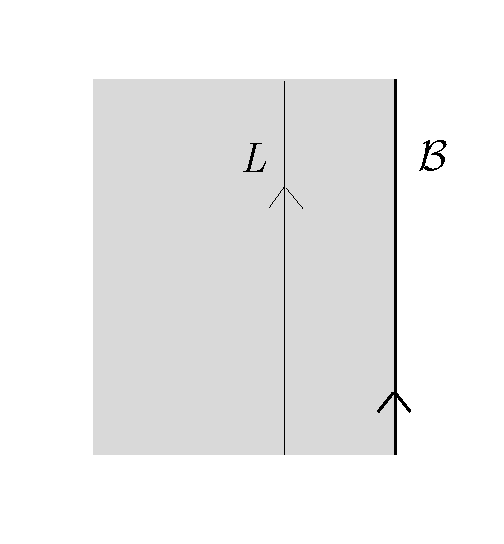
\includegraphics[width=3.5in]{gla8-1.pdf}
\end{center}
\caption{线算符 $L$ 接近由膜 $\B$ 标记的边界. 这给出一个新的复合边界条件\index{boundary-condition@边界条件} $\B'=L\cdot \B$.\label{nuxto}}
\end{figure}

\begin{figure}[!tp]
\begin{center}
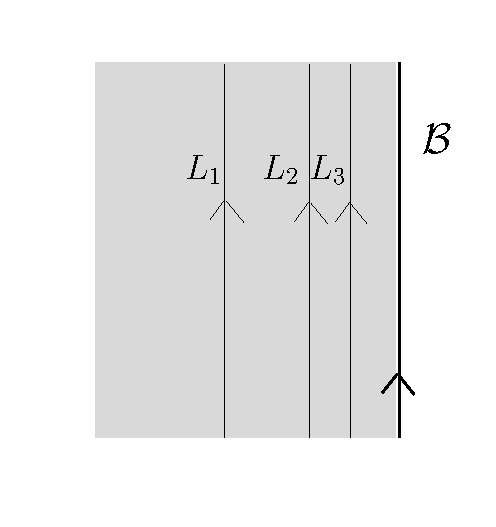
\includegraphics[width=3.5in]{gla8-2.pdf}
\end{center}
\caption{可以将线算符逐个移到边界. 这给出了线算符在膜上的结合性作用. \label{buxto}}
\end{figure}

我们在带边界的二维流形 $\Sigma$ 上研究紧化所得的有效二维理论. 边界条件由膜 $\B$ 定义.（我们将用相同的记号表示膜 $\B$ 和相应的边界条件.）现在的关键是考察线算符接近边界时的行为（图 \ref{nuxto}）. 显然，在二维拓扑场论中，线算符 $L$ 接近具有边界条件 $\B$ 的边界，会产生一个新的复合边界条件 $L\B$. 这给出了线算符在膜上的运算：
\begin{equation}\label{doofus}L \B =\B'. \end{equation}
可以让一串线算符逐个接近边界，从而依次作用于一个膜（图 \ref{buxto}），显然，线算符在膜上的作用具有结合性. 事实上，在目前的情形下，还存在某种交换性. 若 $L,L'$ 是支撑在不同点 $\pp,\pp'\in C$ 处的线算符，那么它们可以在 $\Sigma$ 中彼此穿过而不遇到任何奇点，因此
\begin{equation}\label{loggo} LL'\B=L'L\B. \end{equation}  
但实际上，在四维拓扑场论中，支撑在给定点 $\pp\in C$ 处的线算符局部地与 $\pp$ 无关（从整体上说，若 $\pp$ 沿 $C$ 中不可缩的闭路行进，则可能有非平凡的单值变换\index{monodromy@单值变换}）. 因此，在试图将两个线算符彼此移过时，我们总可以假定它们插入在 $C$ 中不同的点处. 所以，二维理论中源自四维环算符的线算符，即使不加 $\pp\not=\pp'$ 的限制，也彼此对易.

既然我们感兴趣的线算符确实彼此对易，就产生了一个问题：能否在某种意义上将它们同时“对角化”. 要说明这里所需的概念，先要作一些准备.
我们认为，在有效二维描述中，膜 $\B$ 由 $\MH$ 上的一个膜表示. 这个膜是 $A$-膜还是 $B$-膜，取决于我们在底层四维超杨--米尔斯理论中采用哪一种扭曲. 它由 $\MH$ 上的层 $\U$ 描述（根据所考虑的膜，其支撑可以是整个 $\MH$，也可以是一个子流形）. 在膜上有一种自然运算，即将 $\U$ 与一个固定向量空间 $V$ 作张量积. 将这一运算施于膜 $\B$，便得到一个新的膜，记作 $\B\otimes V$；它对应于 $\MH$ 上的层 $\U\otimes V$. 若 $V$ 的维数为 $n$，那么粗略地说，$\B\otimes V$ 是 $n$ 个 $\B$ 的和（这只是一个粗略描述，因为它没有考虑 $V$ 的自同构群 $GL(n,\C)$；利用这个群，可以构造其中 $V$ 非平凡变化的膜族）.
若对某个向量空间 $V$ 有
\begin{equation}\label{zollo}L\B=\B\otimes V \end{equation}
则称膜 $\B$ 是线算符 $L$ 的本征膜\index{eigenbrane@本征膜}.\transnote{这里的 $V$ 只在同构意义下确定：若 $L\B\cong \B\otimes V$，则任何与 $V$ 同构的向量空间同样满足定义，且 $V$ 的自同构群 $GL(n,\C)$ 可用来构造 $V$ 在其中非平凡变化的膜族（上一句已提及）. 在二维拓扑场论中，膜构成一个 $\C$-线性范畴：对象是边界条件，态射是边界上的局域算符；线算符作用于膜给出该范畴的一个张量函子，因此“对角化”只能在范畴层面表述为同构 $L\B\cong \B\otimes V$，而不能写成数值等式，$V$ 的维数相当于 $L$ 在该膜上的“多重数”. 当 $\B$ 是支撑在点 $m$ 处的零维膜时，$V$ 由 $L$ 在 $m$ 处的纤维唯一决定，这正是零维膜作为本征膜时计算最简单的根本原因. [来源：nLab “electric eigenbrane”，\url{https://ncatlab.org/nlab/show/electric+eigenbrane}（Created 2014-07-02；2026-11-19 访问）；[KW]（arXiv:hep-th/0604151）§8（原文 §4.2 所引）；原文 §4.1 式 (4.3) 及上下文.]}

遗憾的是，很难为这一定义中出现的向量空间 $V$ 找到一个方便的术语. 它起着普通矩阵方程 $M\uppsi=\lambda \uppsi$ 中本征值 $\lambda$ 的作用，而它本身又是一个向量空间. 因此，也许可以考虑将 $V$ 称为“本征向量空间”，但遗憾的是，这个短语另有一种更初等的含义.

由于前面解释的原因，$B$-模型的威尔逊算符，或 $A$-模型的 't Hooft 算符，彼此对易，所以可能存在一个膜 $\B$，它是所有威尔逊算符或所有 't Hooft 算符的共同本征膜. 威尔逊算符的共同本征膜，我们称为电本征膜\index{electric-eigenbrane@电本征膜}；'t Hooft 算符的共同本征膜，我们称为磁本征膜\index{magnetic-eigenbrane@磁本征膜}.

数学上表述的几何朗兰兹对应\index{geometric-langlands-correspondence@几何朗兰兹对应} \cite{BD}，在文献 \cite{KW} 中是从 $^L\neg G$ 的威尔逊算符与 $G$ 的 't Hooft 算符之间的对偶性推导出来的. 特别地，这一对偶性将 $^L\neg G$ 的电本征膜映到 $G$ 的磁本征膜. 但是，这些膜具体是什么呢？

\subsection{电本征膜}\label{eleig}

找到电本征膜是直接的. 事实上，更一般地，描述威尔逊算符在膜上的作用也是直接的. 我们将作一个简短的说明，更详细的内容见文献 \cite{KW} 第 8.1 节.
设 $\M$ 是 $C$ 上 $^L\neg G$-丛的模空间\index{moduli-space@模空间}，于是对任意 $m\in \M$，都有一个相应的 $^L\neg G$-丛 $E_m\to C$.
$C$ 上的“万有丛\index{universal-bundle@万有丛}”是一个带联络 $A$ 的丛 $\EE\to C\times \M$，其性质是：对任意 $m\in \M$，$\EE$ 在 $C\times m$ 上的限制同构于 $E_m$.
若 $^L\neg R$ 是 $^L\neg G$ 的不可约表示，则用 $\EE_{^L\neg R}$ 表示表示 $^L\neg R$ 中的伴随丛. 实际上，若 $^L\neg G$ 的中心在表示 $^L\neg R$ 中非平凡地作用，那么 $\EE_{^L\neg R}\to C\times \M$ 不是一个普通向量丛\index{vector-bundle@向量丛}，而是一个扭曲丛，其扭曲由 $\M$ 上一个非平凡的有限阶 $B$-场（或 gerbe）给出. 如文献 \cite{KW} 及下文第 \ref{gerbes} 节所解释的，其物理意义是：表示 $^L\neg R$ 中的威尔逊算符携带一种由该 gerbe 度量的离散电荷\index{electric-charge@电荷}. 这种离散电荷经 $S$-对偶性变换，成为对偶的 't Hooft 算符所携带的离散磁荷\index{magnetic-charge@磁荷}.

万有希格斯丛\index{higgs-bundle@希格斯丛}是一个类似的概念. 设 $\MH$ 是 $C$ 上 $^L\neg G$ 希格斯丛的模空间. 万有希格斯丛是一个带联络 $A$ 的 $^L\neg G$-丛 $\EE_H\to C\times \MH$，并配备一个希格斯场\index{higgs-field@希格斯场} $\phi$，它是 $T^*C
\otimes \mathrm{ad}(\EE_H)$ 的截面（这里的 $T^*C$ 实际上指将 $T^*C$ 从 $C$ 拉回\index{pullback@拉回}到 $C\times \MH$ 所得的丛），使得对任意 $m\in\MH$，$(A,\phi)$ 在 $C\times m$ 上的限制，就是与 $m$ 对应的希格斯丛 $(E,\phi)$.
（同样，一般必须将 $\EE_H$ 理解为扭曲向量丛.）所谓表示 $^L\neg R$ 中的万有希格斯丛，只是指由 $\EE_H $ 通过表示 $^L\neg R$ 得到的伴随丛 $\EE_{H,^L\neg R}\to C\times \MH$.

有了这个概念，就可以一般地描述威尔逊算符在 $B$-膜上的作用. 设 $\B$ 是由层 $\U\to \MH$ 描述的 $B$-膜，$W(^L\neg R,\pp)$ 是表示 $^L\neg R$ 中的威尔逊算符，支撑在点 $\pp\in C$ 处. 那么膜 $W(^L\neg R,\pp)\B$ 由层 $\U\otimes \EE_{H,^L\neg R}|_{\pp\times
\MH}$ 描述. 换言之，威尔逊算符 $W(^L\neg R,\pp)$ 在描述 $B$-膜的层 $\U\to \MH$ 上的作用是
\begin{equation}\label{dotto}\U\to \U\otimes  \EE_{H,^L\neg R}|_{\pp\times
\MH}.   \end{equation} 
这里，$\EE_{H,^L\neg R}|_{\pp\times \MH}$ 就是 $\EE_{H,^L\neg R}$ 在 $\pp\times \MH$ 上的限制；因此它是 $\MH$ 上的一个向量丛，将 $\U\to \MH$ 与这个向量丛作张量积是有意义的.

式 (\ref{dotto}) 中断言背后的直观解释如下. 将图 \ref{nuxto} 中的竖直方向看成“时间”方向. 那么，沿边界延伸的威尔逊算符，就是一个静止的、不依赖于时间的威尔逊算符. 它表示一个处于表示 $^L\neg R$ 中、与周围场相互作用的杂质. 当边界处于由对应于 $m\in\MH$ 的希钦对\index{hitchin-pair@希钦对} $A,\phi$ 描述的经典基态时，外部电荷所感受到的就是这些场. 式 (\ref{dotto}) 只是说，支撑在 $\pp\in C$ 处的威尔逊算符与 $\pp$ 处的场 $A,\phi$ 相互作用.

式 (\ref{dotto}) 表明，一般的 $B$-膜并不是电本征膜，因为 $\EE_{H,^L\neg R}|_{\pp\times
\MH}$ 是 $\MH$ 上的非平凡向量丛，而不是一个常向量空间. 电本征膜应是这样一个膜 $\B$：将 $\EE_{H,^L\neg R}|_{\pp\times
\MH}$ 限制到相应层 $\U$ 的支撑上后，它变为（全纯）平凡的. 若 $\B$ 是支撑在点 $m\in\MH$ 处的零维膜，就会出现这种情形. 此时 $\U$ 是支撑在 $m$ 处的摩天层\index{skyscraper-sheaf@摩天层}，并且
\begin{equation}\U\otimes  \EE_{H,^L\neg R}|_{\pp\times
\MH}\cong \U\otimes  \EE_{H,^L\neg R}|_{\pp\times m}.   \end{equation} 
在右边，$ \EE_{H,^L\neg R}|_{\pp\times m}$ 是 $\EE_{H,^L\neg R}$ 在 $\pp\times m\in
C\times \MH$ 上的限制，特别地，它是一个常向量空间.
因此，支撑在 $m$ 处的零维膜 $\B$ 是一个电本征膜：
\begin{equation}\label{zefor} W(^L\neg R,p)\B=\B\otimes  \EE_{H,^L\neg R}|_{\pp\times m}. \end{equation}

在几何朗兰兹中，我们真正需要的是一个更精确的电本征膜概念. 首先，电本征膜应当是一个膜 $\B$，它是对所有 $^L\neg R$ 和所有 $\pp\in C$ 的全部威尔逊算符 $W(^L\neg R,\pp)$ 的共同本征膜.
同时考虑所有 $\pp$ 的一种方便方法，是将 $\EE_{H,^L\neg R}$ 限制到 $C\times \MH$，而非 $\pp \times \MH$. 于是电本征膜应具有如下性质：
\begin{equation}\label{turnof} \U\otimes  \EE_{H,^L\neg R}|_{C\times
\MH}\cong \U\otimes  V^{^L\neg R},   \end{equation} 
其中 $V^{^L\neg R}$ 是 $C$ 上某个向量丛的拉回. 对任意 $\pp$，将它限制到 $\pp\in C$，便蕴含先前所述的电本征膜性质. 此外，我们要求对不同的 $^LR$，这些陈述彼此相容. 这种相容性是指存在一个主 $^LG$ 丛 $V\to C$，其在表示 $^L\neg R$ 中的伴随丛就是 $V^{^L\neg R}$.

此外，还应指明我们感兴趣的 $\MH$ 上的复结构\index{complex-structure@复结构}. 这里至关重要的是，几何朗兰兹是关于复结构 $J$ 中的电本征膜的陈述；在这个复结构中，$\MH$ 参数化 $C$ 上的平坦 $^LG$ 丛. 复结构 $J$ 中的 $B$-模型，是一个四维拓扑场论约化到二维的结果（如脚注 \ref{partial} 所解释的，这个场论很可能只是部分拓扑的），这意味着威尔逊算符 $W(^L\neg R,\pp)$ 以一种自然方式局部地与 $\pp$ 无关. 这转化为“本征丛” $V^{^L\neg R}\to C$ 或相应主丛 $V\to C$ 上存在一个平坦联络\index{flat-connection@平坦联络}.\transnote{复结构 $J$ 的地位可以用 $\MH$ 的超凯勒三联 $(I,J,K)$ 说明：在 $I$ 中 $\MH$ 是希格斯丛的模空间，而在 $J$、$K$ 中它是 $C$ 上平坦 $^L\neg G$-丛（即局部系统）的模空间. 因此“$J$ 中的电本征膜”就是支撑在某个平坦丛处、其陈-帕顿丛带有平坦联络的膜；经超凯勒旋转，这类膜给出 $D$-模，即几何朗兰兹中的赫克本征层. 这正是原文“几何朗兰兹是关于复结构 $J$ 中的电本征膜的陈述”一语的技术含义，也是第 \ref{magbranes} 节要把电本征膜与磁本征膜纳入同一超凯勒框架的原因. [来源：nLab “Kapustin-Witten TQFT”，\url{https://ncatlab.org/nlab/show/Kapustin-Witten+TQFT}（Last revised 2026-09-28；2026-11-19 访问）；原文 §4.2、§5.1.]}

支撑在点 $m\in \MH$ 处的零维膜满足电本征膜的这些更强条件，其中 $V$ 是在复结构 $J$ 中对应于 $m$ 的平坦丛. 这些性质以一种在几何朗兰兹中自然的方式刻画了零维膜. 不过，本文将利用另一种同样刻画零维膜的性质. 第 \ref{magbranes} 节将更完整地描述这一点，但简要地说，零维膜是一种 $(B,B,B)$ 型的膜（即在 $\MH$ 的复结构 $I, J$ 和 $K$ 中都是 $B$-膜），并且在每个复结构中都是电本征膜.


$S$-对偶性将 $(B,B,B)$ 型的膜映为 $(B,A,A)$ 型的膜（即在复结构 $I$ 中是 $B$-膜，在辛结构 $J$ 或 $K$ 中是 $A$-膜），所以特别地，零维膜的 $S$-对偶将是 $(B,A,A)$ 型的膜. 这些就是我们将研究的磁本征膜.
具体确定零维膜的 $S$-对偶是哪一种膜并不困难. 考虑支撑在点 $m\in\MH$ 处的零维膜 $\B$，该点位于 $^L\neg G$ 的希钦纤维化\index{hitchin-fibration@希钦纤维化}的某个特定纤维 $^L\neg \FF$ 中.
由于 $S$-对偶性在希钦纤维化 $\MH\to \V$ 的纤维上作为 $T$-对偶性起作用，$\B$ 的 $S$-对偶将是支撑在 $G$ 的希钦纤维化的纤维 $\FF$ 上的秩为 1 的 $A$-膜 $\B'$，该纤维对应\footnote{希钦纤维化的纤维由希格斯场 $\varphi$ 的不变多项式的取值参数化. 由于 $^L\neg G$ 和 $G$ 的李代数\index{lie-algebra@李代数}上的不变多项式之间存在自然对应，两个希钦纤维化的纤维之间也存在自然对应. 更准确地说，这一对应涉及对希格斯场的重新缩放，它依赖于规范耦合常数，但不会起本质作用.}于 $^L\neg \FF$.
$\B'$ 由 $\FF$ 上的一个平坦 $\mathrm{Spin}_c$ 结构描述，这个结构编码了 $m$ 在 $^L\neg \FF$ 中的位置.
我们将称它为 $\bf F$ 型的膜.

最终我们将相当明确地理解，为什么支撑在希钦纤维化 $\MH\to \V$ 的一个纤维上的秩为 1 的 $A$-膜是磁本征膜. 不过，我们将首先更好地理解 't Hooft 算符的一般性质.

\subsection{'t Hooft 算符与赫克变换}\label{thecke}

半 BPS 威尔逊算符由复联络 $\A=A+i\phi.$ 的和乐\index{holonomy@和乐}表示. 对闭路 $\mathcal S$，$^L\neg G$ 的表示 $^L\neg R$ 中的半 BPS 威尔逊算符是
\begin{equation}\label{wilop}W(^L\neg R,\mathcal S)=\Tr_{^L\neg R}P\exp\left(-\oint_{\mathcal S}(A+i\phi)\right). \end{equation}

通过 $S$-对偶性转到规范群为 $G$ 的磁性描述后，和乐算符中依赖于 $A$ 的部分，被定义 't Hooft 算符的狄拉克单极子\index{monopole@单极子}奇性取代. 依赖于 $\phi$ 的部分保留下来，在经典层面可以解释为在 $\phi$ 中产生一个奇性.
结果是，半 BPS 't Hooft 算符可以由博戈莫尔尼方程\index{bogomolny-equation@博戈莫尔尼方程}的一个半 BPS 解描述. 准确地说，我们考虑四维时空 $M=\R^3\times \R$，其中 $\R$ 是“时间”方向，由 $s$ 参数化，$\R^3$ 则由三维向量 $\vec x$ 参数化. 那么，静止于 $\vec x=0$ 的 't Hooft 算符，是通过指定场在 $\vec x=0$ 附近应具有的奇性来定义的.
对规范群 $U(1)$ 和荷为 1 的 't Hooft 算符，该解由下式刻画：
\begin{align}\label{charec}F & = \frac{i}{2}\star_3 \frac{1}{|\vec x|}\cr  \phi&=\frac{i}{2|\vec x|}d s. \end{align}
换言之，这是 $F=dA$ 的狄拉克单极子奇性，通过在 $\phi$ 中包含一个类似的点奇性，将它扩充为博戈莫尔尼方程的解.\transnote{式 (4.9) 的归一化可以显式验证：取 $S^2$ 为绕原点的球面，由 $\Delta(1/r)=-4\pi\delta^{(3)}$ 得 $\int_{S^2}F=\pm 2\pi i$（符号取决于定向），即磁通绝对值为 $2\pi$. 在复化约定下这等价于 $e^{\int_{S^2}F}=1$（若换回实场强，则写作 $e^{i\int_{S^2}F}=1$），即狄拉克量子化条件恰好被满足；常数 $i/2$ 就是为使荷为 1 的磁通恰好等于一个量子而选取的. 这也是 §4.4.1 中 $\O\to\O(m\pp)$ 的整数 $m$ 可以与磁荷等同的原因. [来源：nLab “monopole”，\url{https://ncatlab.org/nlab/show/monopole}（Last revised 2026-05-27；2026-11-19 访问；磁荷＝U(1) 主丛的第一陈类）；原文 §4.3 式 (4.9)、§4.4.1.]}

一般地 \cite{Kapustintwo}，规范群 $G$ 的任意半 BPS 't Hooft 算符，是通过选取一个同态
\begin{equation}\label{pickhom}\rho:U(1)\to G, \end{equation}
并利用这一同态将阿贝尔解 (\ref{charec}) 嵌入 $G$ 来定义的.
在朗兰兹对偶性或 GNO 对偶性中，以下陈述非常基本：在共轭意义下，同态 $U(1)\to G$ 由对偶群 $^L\neg G$ 的优势最高权分类，等价地，由 $^L\neg G$ 的不可约表示 $^L\neg R$ 分类. 因此，$G$ 的 't Hooft 算符与 $^L\neg G$ 的威尔逊算符存在自然对应.\transnote{这一分类在数学上称为 GNO（Goddard–Nuyts–Olive）对偶：$G$ 的磁荷（单极子荷）取值于 $\pi_1(G)$ 的对偶，而在共轭意义下，从 $U(1)$ 到 $G$ 的同态 $\rho$ 恰由一个优势余权刻画，对偶地由 $^L\neg G$ 的一个优势最高权 $\lambda$ 刻画；二者以 $\langle\lambda,\rho\rangle\in\Z$ 配对，这个整数就是 't Hooft 算符的荷. 因此 $G$ 的 't Hooft 算符的荷可以用 $^L\neg G$ 的最高权来标记，并与 $^L\neg G$ 的威尔逊算符一一对应. 原文只陈述这一对应，未展开配对的具体构造. [来源：nLab “’t Hooft operator”，\url{https://ncatlab.org/nlab/show/}\%27t+Hooft+operator（Last revised 2025-07-04；2026-11-19 访问）；[KW]（arXiv:hep-th/0604151）§6.2（该页所引）；原文 §4.3 式 (4.10).]}

$A$-模型可观测量的计算，基本上是求解具有适当未破缺超对称\index{supersymmetry@超对称}性的场构型所满足的方程，然后计数其解，或对解空间作适当量子化. 为理解 't Hooft 算符在膜上的作用，所要考虑的基本问题如下. 四维时空为 $\Sigma\times C$，其中 $\Sigma$ 是带边界的二维流形.
所考虑的 't Hooft 算符平行于 $\Sigma$ 的边界延伸，如图 \ref{nuxto} 所示. 在边界附近，可以将 $\Sigma$ 分解为 $I\times \R$，其中 $\R$ 是沿边界延伸的“时间”方向，$I$ 是带边界的一维流形. 与理解 't Hooft 算符在膜上的作用有关的超对称场不依赖于时间，因此它们是三维规范理论\index{gauge-theory@规范理论}方程的解，具体地说，是 $I\times C$ 上的方程的解. 虽然紧致的带边界一维流形 $I$ 必然有两个端点，我们只关注其中一个端点，并将它记为 $\partial I$，因为我们希望研究靠近 $\Sigma$ 的某个给定边界的 't Hooft 算符.

我们将简要描述必须满足的超对称方程，更详细的内容见文献 \cite{KW}.
当希格斯场 $\phi$ 中切于 $C$ 的部分沿 $\partial I$ 消失时，相关方程最为熟悉. 在这种情形下，可以假定 $\phi$ 唯一非零的分量是“时间”方向上的分量 $\phi_s$；它被迫非零，因为它在 't Hooft 算符的位置实际上具有奇异行为（式 (\ref{charec})）. 可以证明一个消失定理：在行为良好的解中，$A$ 的“时间”分量 $A_s$ 消失.
于是，这些方程约化为三维流形 $I\times C$ 上关于联络 $A$ 和伴随表示值标量场 $\phi_s$ 的方程.
可以证明，这些方程就是博戈莫尔尼方程：
\begin{equation}\label{zoddo} F=\star D\phi_s. \end{equation}
存在 't Hooft 算符时，相关的博戈莫尔尼方程解将具有狄拉克单极子奇性.
（关于博戈莫尔尼方程的多数文献讨论光滑解，但也有大量文献讨论具有这种奇性的解 \cite{kronheimermon,polo,golo,golo2,latwein,bais,hanwit,cherkis}.）

在 $\phi$ 的切向部分不消失的更一般情形下，仍然可以证明关于 $A_s$ 和 $\phi$ 的“法向”分量，即沿 $I$ 的分量的消失定理. 用实变量 $y$ 参数化 $I$，并在 $C$ 上选取局部坐标 $z$，会比较方便.（对 $C=\R^2$，$y$ 和 $z$ 可以通过 $y=x^1$、$x=x^2+ix^3$，与 $\T\times C=\R^3$ 上的欧氏坐标联系起来.）消失定理表明，我们可以令 $A_s=\phi_y=0$. 超对称方程（按文献 \cite{KW} 式 (3.29) 的记号取 $t=1$；这是研究 $A$-模型的一个方便取值）一般写为
\begin{equation}\label{irko}0=F-\phi\wedge\phi+\star D_A\phi = D_A\star \phi, \end{equation}
其中 $D_A=d+[A,\cdot]$，$\star $ 为霍奇星算符. 当专门考虑 $A_s=\phi_y=0$ 的情形时，其余场的方程可以表述如下（这一描述是在文献 \cite{WittenKhov} 第 3.6 节中引入的，并被用来寻找这些方程的一些有趣解）. 定义三个算符
\begin{align}\label{doff}\D_1 & = \frac{D}{D\bar z}=\partial_{\bar z}  +[A_{\bar z},\,\cdot\, ]\cr
               \D_2& =D_y-i[\phi_s,\,\cdot\,]      \cr 
                  \D_3&=[\phi_z,\,\cdot\,] ,  \end{align}  
以及“矩映射\index{moment-map@矩映射}”
\begin{equation}\label{zolff}\mu=\sum_{i=1}^3[\D_i,\D_i^\dagger].\end{equation} 
那么，超对称构型的方程可以写为一个“复方程”
\begin{equation}\label{woff} [\D_i,\D_j]=0,~~1\leq i<j\leq 3,\end{equation}
和一个“矩映射条件”
\begin{equation}\label{old} \mu=0.\end{equation}  
将这一组合方程组称为扩展博戈莫尔尼方程\index{extended-bogomolny-equation@扩展博戈莫尔尼方程}会很方便，其中的扩展是指包含了希格斯场 $\varphi=\phi_z\, dz$.\transnote{这里的两组写法是同一物理内容的两种形式：式 (4.11) 是 3 维欧氏空间上的博戈莫尔尼方程（即 4 维自对偶杨--米尔斯方程经平移不变约化到 3 维所得），而 $D_1,D_2,D_3$ 是超凯勒商构造中的标准记号——$D_1$ 是 $\bar\partial$ 型算符，$D_2,D_3$ 分别是另外两个复结构中的 $\bar\partial$ 型算符，$\mu=\sum_i[D_i,D_i^\dagger]$ 则是相应的超凯勒矩映射. 于是“复方程 $[D_i,D_j]=0$ 加 $\mu=0$”就是把希钦方程（从而把 $\MH$ 的复结构）写成三个复结构的统一形式，这也是原文说这些条件“在相当简单的应用中都满足”的原因. 另外，原文按 [1] 式 (3.29) 取 $t=1$，$t$ 是 [1] 中那一族拓扑扭曲理论的参数，取 $1$ 是 [1] 中为研究 A-模型而选取的方便值. [来源：原文 §4.3 式 (4.11)–(4.16) 及上下文；nLab “Bogomolny equation”，\url{https://ncatlab.org/nlab/show/Bogomolny+equation}（Created 2019-10-14；2026-11-19 访问）；[KW]（arXiv:hep-th/0604151）§3.6（原文所引）.]}

复方程 $[\D_i,\D_j]=0$ 在 $G_\C$ 值规范变换下不变. 在适当的半稳定\index{semistability@半稳定}性条件下，这些条件在相当简单的应用中（例如本文将考虑的应用）都满足，我们预期，复方程的解模去复值规范变换，等价于完整方程组 $[\D_i,\D_j]=\mu=0$ 的解模去 $G$ 值规范变换. 因此，要确定解的模空间，主要需要理解复方程 $[\D_i,\D_j]=0$.

若 $\varphi=0$，则显然 $\D_3=0$. 其余方程 $[\D_1,\D_2]=[\D_1,\D_1^\dagger]+[\D_2,\D_2^\dagger]=0$ 就是以一种可能不太熟悉的方式写出的博戈莫尔尼方程 (\ref{zoddo}).
不过，博戈莫尔尼方程的这种写法非常便于应用到几何朗兰兹中.

首先，必须回顾：黎曼曲面 $C$ 上的 $G$-丛 $E\to C$ 的任意联络，其 $(0,1)$ 部分都定义一个 $\bar\partial$ 算符，从而将 $E$（更准确地说，是其复化）变成一个全纯 $G_\C$-丛. 因此，特别地，在任意给定的 $y$ 值处，算符 $\D_1$ 就是这样的 $\bar\partial $ 算符，并赋予丛 $E$ 一个全纯结构. 方程 $[\D_1,\D_2]=0$ 告诉我们，在共轭意义下，算符 $\D_1=D_{\bar z}$ 与 $y$ 无关，因为
\begin{equation}\label{zobo}\frac{\partial}{\partial y}D_{\bar z}=-[A_y+i\phi_s,D_{\bar z}].  \end{equation}
因此，只要满足这个方程，丛 $E$ 的全纯结构就与 $y$ 无关.

现在，假设在某个点 $y=y_0$、$z=z_0$ 处有一个 't Hooft 算符. 在该点，博戈莫尔尼方程中有一个德尔塔函数源，条件 $[\D_1,\D_2]=0$ 不成立. 穿过 $y=y_0$ 时，丛 $E$ 的全纯类型实际上会发生跳跃；在 $y>y_0$ 时为一种类型，在 $y<y_0$ 时为另一种类型. 但是，与 't Hooft 算符相关的奇性只发生在 $C$ 中的一个点 $z=z_0$ 处.
若从 $C$ 中去掉这一个点，那么即使穿过 $y=y_0$，丛 $E $ 的全纯结构也不变.

在几何朗兰兹纲领中，对全纯 $G$-丛 $E\to C$ 的一种修正，如果从 $C$ 中去掉单个点 $\pp$ 后就成为平凡的，就称为 $E$ 在 $\pp$ 处的赫克修正.（这个术语源于与数论中赫克算符的类比.）
因此，'t Hooft 算符在其插入的 $C$ 中的点处，诱导全纯 $G$-丛 $E$ 的一个赫克修正.

几何朗兰兹的数学研究方法中的一个重要事实是，$G$-丛可能有不同类型的赫克修正，而这些可能的类型由对偶群 $^L\neg G$ 的不可约表示 $^L\neg R$ 的选择来分类. 我们所描述的正是对此的物理解释：赫克修正的可能类型由 't Hooft 算符的选择决定，而这个选择确定博戈莫尔尼方程解中奇性的精确性质.
此外，'t Hooft 算符确实由 $^L\neg R$ 的选择来分类.\transnote{在数学侧，$\pp$ 处的赫克修正的参数空间可以等同于仿射 Grassmannian $\mathrm{Gr}_G$ 的一个 Schubert 胞腔：$\mathrm{Gr}_G$ 的对象是形式圆盘 $D=\mathrm{Spec}\,\C[[z]]$ 上的 $G$-丛连同在穿孔圆盘 $D^*$ 上的平凡化，而平凡化在 $\pp$ 处允许的极点阶数由一个优势余权（对偶地，$^L\neg G$ 的一个优势最高权）标记，对应的 Schubert 胞腔就是这一类型的全部赫克修正. 因此“赫克修正的类型”天然由 $^L\neg G$ 的最高权分类；当该权微小、相应胞腔紧致时不需要单极子冒泡，这正是下一小节判据的几何来源. 原文只引 [1] 的 §9、§10，未给出仿射 Grassmannian 的构造. [来源：nLab “affine Grassmannian”，\url{https://ncatlab.org/nlab/show/affine+Grassmannian}（Last revised 2023-08-15；2026-11-19 访问）；[KW]（arXiv:hep-th/0604151）§9–§10（原文 §4.3 所引）；原文 §4.3.]}

将希格斯场 $\varphi$ 纳入这一讨论并不困难. 在固定的 $y$ 处，有方程 $[\D_1,\D_3]=0$，它告诉我们 $[D_{\bar z},\varphi]=0$，换言之，$A_{\bar z},\varphi$ 是一个希钦对，并确定一个希格斯丛；我们将它看作由全纯丛\index{holomorphic-bundle@全纯丛} $E$ 及 $\varphi\in H^0(C,K\otimes\ade)$ 组成的一对.
方程 $[\D_2,\D_1]=[\D_2,\D_3]=0$，即
\begin{equation}\label{dolgo}[D_y-i\phi_s,D_{\bar z}]=[D_y-i\phi_s,\varphi]=0 \end{equation}
告诉我们，远离可能存在的 't Hooft 算符的位置时，希格斯丛 $(E,\varphi)$ 的全纯类型与 $y$ 无关.
若在 $y=y_0$ 及点 $\pp\in C$ 处存在一个 't Hooft 算符，对 $(E,\varphi)$ 的全纯类型就会在 $y=y_0$ 处跳跃，但这种跳跃在从 $C$ 中去掉点 $\pp$ 后就成为平凡的. 我们可以这样描述它：穿过 $y=y_0$ 时，对 $(E,\varphi)$ 在点 $\pp\in C$ 处经历一次赫克修正.

若只忘掉 $\varphi=\D_3$ 及它所参与的方程，仅保留 $\D_1,D_2$ 和条件 $[\D_1,\D_2]=0$，就会看到，$(E,\varphi)$ 的赫克修正特别包含 $E$ 的一个普通赫克修正. 现在重新考虑 $\varphi$，方程 $[\D_1,\D_1]=[\D_2,\D_3]=0$ 意味着，在 $y\not=y_0$ 时，$(E,\varphi)$ 的全纯类型与 $y$ 无关. 但是，穿过 $y=y_0$ 时会发生什么？
条件 $0=[\D_2,\D_3]=[D_y-i\phi_s,\varphi]$ 决定穿过 $y=y_0$ 时 $\varphi$ 会怎样变化. 例如，若在 $y>y_0$ 时一般地选取 $\varphi$，那么在 $y<y_0$ 时，它将在 $z=z_0$ 处具有一个极点.
这一重要事实将在第 \ref{inco} 节解释. 由这一事实可知，希钦对 $(E,\varphi)$ 在指定点 $\pp\in C$ 处的可能赫克修正，是 $E$ 在 $\pp$ 处的可能赫克修正的一个子集. 我们将 $(E,\varphi)$ 的赫克修正称为 $E$ 的 $\varphi$-不变赫克修正. 这一术语的理由将会变得清楚. 数学上已经研究过希格斯丛 $(E,\varphi)$ 的赫克修正 \cite{donagip}.

在理解对 $(E,\varphi)$ 的赫克修正之前，应当先熟悉 $\varphi=0$ 这一特殊情形下 $E$ 本身的赫克修正.
读者或许可查阅文献 \cite{KW} 第 9 节和第 10 节，那里给出了一个介绍. 这里我们只回顾几个事实，它们是研究磁本征膜时所需的最少准备.


\subsection{基本例子}\label{basics}

\subsubsection{$G=U(1)$}\label{guone}

所要考虑的最基本情形是群 $G=U(1)$. 在这种情形下，$E$ 是一个复线丛\index{line-bundle@线丛}，记作 $\L$.
对某个 $y_0$，当 $y\not=y_0$ 时，$\L$ 的同构类型将保持不变. 当 $y<y_0$ 时，将 $\L$ 记作 $\L_-$；当 $y>y_0$ 时，将它记作 $\L_+$.

穿过 $y=y_0$ 时，$\L$ 会以一种除点 $\pp\in C$ 外处处平凡的方式发生修正.
我们可以在 $\pp$ 的一个邻域中选取 $\L_-$ 的平凡化\index{trivialization@平凡化}，从而将它等同于平凡线丛 $\O$.
在 $\pp$ 之外，利用联络 $D_y-i\phi_s$ 沿 $y$ 方向作平行移动，$\L_-$ 的平凡化便确定 $\L_+$ 的一个自然平凡化. 换言之，若在 $y<y_0$ 时，$\L_-$ 的一个全纯截面 $s$ 在 $\pp$ 的邻域 $U$ 中给出 $\L_-$ 的平凡化，则将 $s$ 平行移动到 $y>y_0$，会在 $U\backslash \pp$ 上（即从 $U$ 中去掉点 $\pp$ 后）给出 $\L_+$ 的平凡化.
因此，在 $U\backslash p$ 上，$\L_+$ 自然地等同于 $\O$.

但 $\O$ 的这一平凡化不一定能延拓过点 $\pp$. 一般的可能性是，在平行移动到 $y>y_0$ 后，截面 $s$ 可能在 $\pp$ 处具有一个 $m$ 阶零点（或 $-m$ 阶极点），其中 $m$ 为某个整数.
因此，在将 $\L_-$ 等同于 $\O$ 后，可以将 $\L_+$ 等同于 $\O(m\pp)$.
这里，$\O(m\pp)$ 是这样一个线丛：它在 $\pp$ 附近的局部截面，是允许在 $\pp$ 处有 $m$ 阶极点（或要求有 $-m$ 阶零点）的全纯函数.

文献 \cite{KW} 第 4.5 节解释了，赫克变换\index{hecke-transformation@赫克变换} $\O\to \O(m\pp)$ 是在点 $\pp\times y_0\in
C\times \R$ 处插入一个磁荷为 $m$ 的 't Hooft 算符 $T(m)$ 的结果.（若希望指明它插入的点 $\pp\in C$，则将这一 't Hooft 算符记作 $T(m;\pp)$.）
证明这一点的基本思想是，这样一个 't Hooft 算符产生 $m$ 个单位的磁通. 在点 $\pp\in C$ 处产生 $m$ 个单位磁通的运算，在代数几何中描述为赫克变换 $\O\to \O(m\pp)$.\transnote{更定量地说，$\O(m\pp)$ 与 $\O$ 的差别由第一陈数给出：$c_1(\O(m\pp))=m$，而 $\int_C c_1=m$ 正是穿过 $C$ 的磁通数（以式 (4.9) 的 $2\pi i$ 为单位）. 线算符可以融合，$T(m_1)\cdot T(m_2)=T(m_1+m_2)$，对应地 $\O\to\O(m_1\pp)\to\O((m_1+m_2)\pp)$，磁荷相加；$m<0$ 时修正方向相反. 这给出了 $U(1)$ 情形“赫克修正的类型就是磁荷”的完整字典. [来源：nLab “monopole”，\url{https://ncatlab.org/nlab/show/monopole}（Last revised 2026-05-27；2026-11-19 访问；磁荷＝第一陈类）；[KW]（arXiv:hep-th/0604151）§4.5（原文 §4.4.1 所引）；原文 §4.4.1.]}

\subsubsection{$G=U(2)$}\label{gutwo}

作为第二个例子，取 $G=U(2)$. 丛 $E$ 现在是秩为 2 的复向量丛，当 $y<y_0$ 或 $y>y_0$ 时，分别将它记作 $E_-$ 或 $E_+$.
由于全纯向量丛是局部平凡的，可以在 $y<y_0$ 时选取一个将 $E_-$ 等同于 $\O\oplus \O$ 的同构.
现在，一个基本的赫克运算将 $E_-$ 变为
\begin{equation}\label{zobbox} E_+ =\O(\pp)\oplus \O  \end{equation}
这里 $y>y_0$. 如文献 \cite{KW} 所解释的，这是由与 $^L\neg U(2)\cong U(2)$ 的自然二维表示对偶的 't Hooft 算符所实现的赫克变换. 可以将该表示看成 $U(2)$ 的最高权为 $^Lw=(1,0)$ 的表示.
我们将相应的 't Hooft 算符记作 $T(^Lw)$（或 $T(^Lw; \pp)$）.
我们将由 $T(^Lw)$ 诱导的赫克变换称为 $^Lw$ 型的赫克变换.

式 (\ref{zobbox}) 展示的，是 $^Lw=(1,0)$ 时由 $T(^Lw)$ 诱导的赫克变换的一个特例.
它之所以是特例，是因为使用了将 $E_-$ 分解为 $\O\oplus \O$ 的一个特定分解.
更一般地，我们不必说 $E_+$ 的截面是允许第一个分量具有一阶极点的 $\O\oplus\O$ 的截面，而可以允许两个分量的某个指定线性组合具有一阶极点.
为此，选取一对不同时为 0 的复数 $(u,v)$，并规定 $E_+$ 的截面是一对 $(f,g)$，它在 $\pp$ 之外定义 $\O\oplus \O$ 的截面，允许 $f$ 和 $g$ 在 $\pp$ 处有一阶极点，但该极点的留数必须是 $(u,v)$ 的倍数.
写成公式，若 $z$ 是 $C$ 上在 $\pp$ 处有一阶零点的全纯函数，则要求
\begin{equation}\label{zummo} (f,g)=(f_0,g_0)+\frac{\lambda}{z}(u,v), \end{equation}
其中 $f_0$ 和 $g_0$ 在 $\pp$ 处全纯，$\lambda$ 是一个可以非零的复数.
由此过程定义的丛 $E_+$ 显然只依赖于 $(u,v)$ 的整体缩放等价类，因此，从 $E_-$ 出发作 $(1,0)$ 型赫克变换，以这种方式构造的丛 $E_+$ 的族，由一个 $\CP^1$ 参数化.\transnote{这个 $\CP^1=\Bbb P(E_{-,\pp})$ 是仿射 Grassmannian $\mathrm{Gr}_{U(2)}$ 中对应于微小权 $(1,0)$ 的 Schubert 胞腔：$\pp$ 处的一阶极点配上留数方向 $(u,v)$，正好给出该胞腔的全部（有限维的）参数. 对 $U(N)$ 的微小权 $(1,\dots,1,0,\dots,0)$，同样的构造给出有限维的 $\mathbf{Gr}(k,N)$（见式 (4.30) 之后的讨论），因为此时 Schubert 胞腔紧致；一般权的 Schubert 胞腔不紧致，其紧化需要粘上较低权的胞腔，物理上就是下一段所说的单极子冒泡. [来源：nLab “affine Grassmannian”，\url{https://ncatlab.org/nlab/show/affine+Grassmannian}（Last revised 2023-08-15；2026-11-19 访问）；[KW]（arXiv:hep-th/0604151）§10（原文 §4.4.2 所引）；原文 §4.4.2.]}
为便于后文引用，将截面看成列向量而非行向量来改写式 (\ref{zummo})会比较方便.
于是，$E_+$ 的全纯截面 $s$ 具有形式
\begin{equation}\label{onkey}s=s_0+\frac{\lambda}{z}\begin{pmatrix}u \cr v\end{pmatrix}, \end{equation}
其中 $s_0$ 是 $E_-$ 的全纯截面，列向量 $\begin{pmatrix} u\cr v\end{pmatrix}$ 现在表示齐次坐标为 $u,v$ 的 $\CP^1$ 中的一个元素.


不选取 $E_-$ 的任何局部平凡化，也可以更内在地得到这一结果.
用 $E_{-,p}$ 表示 $E_-$ 在 $p$ 处的纤维，并选取非零向量 $\bb\in E_{-,p}$.
然后，规定 $E_+$ 在 $p$ 附近的截面具有形式
\begin{equation}s=s_0+\frac{\bb}{z}\lambda. \end{equation}
以此来刻画 $E_+$.
因此，我们允许一阶极点，但其留数必须是 $\bb$ 的倍数.
这样得到的丛只依赖于 $\bb$ 的缩放等价类，所以这种丛的族是对二维向量空间 $E_{-,p}$ 作射影化所得的一个 $\CP^1$.
将 $E_{-,p}$ 的这一射影化记作 $\Bbb P(E_{-,p})$.

因此，对于给定丛 $E_-\to C$ 和指定点 $p\in C$，存在一个自然的在该点作 (1,0) 型赫克修正的空间.
这个空间是一个紧致光滑流形，是一个自然同构于 $\Bbb P(E_{-,p})$ 的 $\CP^1$.

在一定范围内，可以用类似方式处理 $U(2)$ 的任意 't Hooft 算符.
$^L\neg U(2)\cong U(2)$ 的任意表示的最高权，由一对整数 $(n,m)$ 给出.
外尔群的作用交换这两个权，因此通过一个外尔变换，可以取 $n\geq m$.

$(n,m)$ 型赫克修正的一个例子，是将 $E_-=\O\oplus \O$ 映为
\begin{equation}\label{doffy}E_+=\O(n\pp)\oplus \O(m\pp). \end{equation}
的修正.
这是在 $\pp$ 处作 $(n,m)$ 型赫克修正的一个特例.
所有这种赫克修正组成的族具有复维数 $n-m$.
然而，与上面处理的 $n-m=1$ 情形相比，这里有一个重要的复杂之处.
当 $n-m\geq 2$ 时，$(n,m)$ 型赫克修正的空间并不紧致；更恰当地说，它有一个自然的紧化，需要允许较低权的赫克修正（即 $1\leq k\leq (n-m)/2$ 时权为 $(n-k,m+k)$ 的修正）.
从 't Hooft 算符的观点看，这一紧化涉及“单极子冒泡\index{monopole-bubbling@单极子冒泡}”：在一个 't Hooft 算符的场中，光滑的 BPS 单极子在靠近该 't Hooft 算符的位置缩小并消失.\footnote{这类冒泡对于四维杨--米尔斯瞬子而言比较熟悉，但对于 BPS 单极子可能不太熟悉，因为在没有 't Hooft 算符时它不会发生.
更准确地说，对规范群 $U(2)$，只有存在权满足 $n-m\geq 2$ 的 't Hooft 算符时，才会发生这种现象.}
当 $n-m\geq 2$ 时，$(n,m)$ 型赫克修正的紧化空间具有与单极子冒泡相关的奇点.
在几何朗兰兹文献中，给定类型的赫克修正空间称为舒伯特胞腔，其紧化称为（仿射格拉斯曼流形中的）舒伯特闭链.\transnote{从物理上看，紧化的粘合点对应“在一个 't Hooft 算符的背景中，一个光滑 BPS 单极子收缩到零尺度”：单极子带磁荷 $k$ 时会把部分磁荷交给 't Hooft 算符，使原来的权 $(n,m)$ 变为较低的权（例如 $(n-k,m+k)$），这正是上一段所说的“较低权”修正；单极子半径趋于零时总磁荷守恒，所以紧化中只会出现同一总荷的较低权修正. 由于需要 $1\le k\le (n-m)/2$，只有 $n-m\ge 2$ 时才会发生冒泡，这解释了为何 $n-m\le 1$（微小情形）的修正空间本身就是紧的、一个 Schubert 胞腔就够了. [来源：[KW]（arXiv:hep-th/0604151）§10（原文 §4.4.2 所引）；nLab “monopole”，\url{https://ncatlab.org/nlab/show/monopole}（Last revised 2026-05-27；2026-11-19 访问）；原文 §4.4.2 式 (4.23) 及脚注.]}

关于这些问题的介绍，可以在文献 \cite{KW} 第 10 节找到.
不过，这里我们希望避开与单极子冒泡以及赫克修正紧化空间的奇点有关的复杂情况.
因此，我们将只限于满足 $n-m\leq 1$ 的 't Hooft 算符 $T(n,m)$.

条件 $n-m\leq 1$ 等价于说，$^L\neg U(2)=U(2)$ 的最高权为 $(n,m)$ 的表示是“微小”的.
若紧李群 $^L\neg G$ 的一个表示的权构成外尔群的单个轨道，则称该表示是微小的.
$U(2)$ 的最高权为 $(m,m)$ 的表示是一个一维表示，其中 $g\in U(2)$ 的作用为乘以 $(\det g)^m$.
最高权为 $(m+1,m)$ 的表示是一个二维表示，其中（将 $g$ 看成 $2\times 2$ 矩阵）$g$ 的作用为乘以 $g(\det g)^m$.
这些都是微小表示\index{minuscule-representation@微小表示}，因为例如刚才提到的二维表示恰有两个权，它们由一个外尔变换交换.\transnote{判断微小有一个实用判据：不可约表示 $^L\neg R$ 微小，当且仅当其维数等于最高权的 Weyl 群轨道大小，等价地，当且仅当其所有权同属一个 Weyl 轨道. 对 $U(2)$，权为 $(n-j,m+j)$（$j=0,1,\dots,n-m$），Weyl 群 $S_2$ 交换两个分量，所以恰好当 $n-m\le 1$ 时所有权在同一轨道上——这与原文的条件 $n-m\le1$ 一致. 特别地，$SU(2)$ 只有二维表示微小；$SO(3)$ 的中心平凡，故没有非平凡的微小表示（与“微小表示对应中心特征标”的一般事实相符）. [来源：原文 §4.4.2（微小表示的定义及式 (4.23) 之后的讨论）；[KW]（arXiv:hep-th/0604151）§10；2026-11-19 核对.]}

一般地，设 $^L\neg R$ 是任意紧群 $^L\neg G$ 的不可约表示，其最高权为 $^Lw$.
$^Lw$ 型赫克修正的空间紧致，或等价地，在 't Hooft 算符 $T(^Lw)$ 的场中没有单极子冒泡，当且仅当表示 $^L\neg R$ 是微小的.
若 $^L\neg G$ 半单，则微小表示与 $^L\neg G$ 中心的非平凡特征标一一对应.
实际上，按 $^L\neg G$ 中心的某个给定特征标变换的最小 $^L\neg G$ 表示，总是微小的.
例如，$^L\neg G=SU(2)$ 恰有一个非平凡微小表示，即二维表示.
（由于 $SU(2)$ 的外尔群只有两个元素，$SU(2)$ 的维数大于 2 的表示不可能是微小的.）
群 $^L\neg G=SO(3)$ 没有非平凡微小表示.

\subsubsection{$G=SO(3)$ 或 $SU(2)$}\label{morz}

现在，考虑 $G$ 为 $SO(3)$ 或 $SU(2)$ 的情形.

$G=SO(3)$ 的对偶群是 $^L\neg G=SU(2)$.
在专门讨论 $SU(2)$ 之前，先对 $U(N)$ 和 $SU(N)$ 作一些说明，这些说明将在第 \ref{zoff} 节用到.

$U(N)$ 的权格由整数 $m_1,\dots, m_N$ 构成的 $N$ 元组 $(m_1,m_2,\dots, m_N)$ 张成.
外尔群通过置换作用，因此在相差一个外尔变换的意义下，可以施加优势权条件 $m_1\geq m_2\geq \dots\geq m_N$.

$SU(N)$ 的权格由类似的 $N$ 元组 $(m_1,m_2,\dots, m_N)$ 张成，但现在取 $m_i\in \Z/N$，并满足 $m_i-m_j\in \Z$，且要求 $\sum_im_i=0$.
外尔群仍通过置换作用，优势权仍满足 $m_1\geq m_2\geq\dots\geq m_N$.

将这一描述专门用于 $^L\neg G=SU(2)$，就意味着优势权具有 $^Lw=(n/2,-n/2)$ 的形式，其中 $n$ 为整数.
现在，考虑与 't Hooft 算符 $T(^L\neg w)$ 相关的赫克修正.
粗略地说，在 $p$ 处的一个典型的这种赫克修正，将丛 $E_-=\O\oplus \O$ 映为
\begin{equation}\label{lapel}E_+=\O(n\pp/2)\oplus \O(-n\pp/2).  \end{equation}

然而，我们应当问：若 $n$ 为奇数，从而 $n/2\notin\Z$，这意味着什么？
答案是，当 $^L\neg G=SU(2)$ 时，$G=SO(3)$.
群 $SO(3)$ 没有二维表示，所以不应试图将 $G$-丛看成秩为 2 的复向量丛.
要作出严格的陈述，应当考虑 $SO(3)$ 的伴随表示中的伴随丛 $V=\ad_0(E)$，而不应考虑秩为 2 的复向量丛 $E$.
（对于具有对偶丛 $E^*$ 的秩为 $N$ 的复向量丛 $E$，用 $\ad(E)$ 表示 $E\otimes E^*$，用 $\ad_0(E)$ 表示 $E\otimes E^*$ 的无迹部分.）
注意，$V$ 配备一个全纯、非退化的双线性型，它来自对 $v,v'\in \ad_0(E)$ 定义的 $(v,v')=\Tr\,vv'$.
对 $E_-=\O\oplus \O$，有 $V_-=\ad(E_-)
=\O\oplus \O\oplus\O$；对由式 (\ref{lapel}) 非正式定义的 $E_+$，有 $V_+=\ad_0(E_+)=\O\oplus \O(n\pp)\oplus \O(-n\pp)$.
因此，$T(^Lw)$ 在 $SO(3)$ 丛 $V$ 上作用的一个典型例子为
\begin{equation}\label{apel}\O\oplus\O\oplus \O\to \O\oplus \O(n\pp)\oplus \O(-n\pp). \end{equation}
$SO(3)$ 丛 $\O\oplus \O(n\pp)\oplus \O(-n\pp)$ 上的二次型将 $\O$ 与自身配对，将 $\O(n\pp)$ 与 $\O(-n\pp)$ 配对，所以特别地，$\O(n\pp)$ 和 $\O(-n\pp)$ 是迷向子空间.

$^L\neg G=SU(2)$ 唯一的非平凡微小表示对应于 $n=1$，所以 $^Lw=(1/2,-1/2)$ 是 $SU(2)$ 的二维表示的最高权.
于是，式 (\ref{apel}) 给出相应 't Hooft 算符 $T(^Lw)$ 在 $SO(3)$ 丛上作用的局部形式.
不过，用 $SO(3)$ 丛 $V$ 所作的描述虽然严格，却往往冗长；通过 $V=\mathrm{ad}_0(E)$ 将 $SO(3)$ 丛 $V$ 与一个可能具有非平凡行列式的秩为 2 的复向量丛 $E$ 联系起来，会更简单.
这样做时，将 $E$ 与线丛 $\L$ 作张量积没有影响（因为 $\ad_0(E)$ 自然同构于 $\ad_0(E\otimes \L)$）.
因此，不必说 $T(^L\neg w)$ 将 $E_-=\O\oplus \O$ 映到式 (\ref{lapel}) 中所写的形式表达式；同样可以在形式上与 $\L=\O(n\pp/2)$ 作张量积，然后说
\begin{equation}\label{zapel} E_+=\O(n\pp)\oplus \O,\end{equation}
这里仍须理解，我们真正感兴趣的是 $V_+=\ad(E_+)$，而非 $E_+$.

因此，对于 $SU(2)$ 的微小权\index{minuscule-weight@微小权} $(1/2,-1/2)$，即 $^Lw$，描述 't Hooft 算符 $T(^Lw)$ 的作用的最方便方式，是说它局部地将 $E_-=\O\oplus \O$ 映为
\begin{equation}\label{inrtz}E_+=\O(\pp)\oplus \O. \end{equation}
这样说时，我们始终记得，从 $E_-$ 到 $E_+$ 的这个变换，是描述从 $V_-=\ad_0(E_-)=\O\oplus \O\oplus \O$ 到 $V_+=\ad_0(E_+)=\O\oplus \O(\pp)\oplus \O(-\pp)$ 的赫克修正的一种简写方式.\transnote{用 $V=\ad_0(E)$ 而不直接用 $E$ 的必要性在于：把 $E$ 换成 $E\otimes\L$（$\L$ 为任意线丛）不改变 $\ad_0(E)$，因此 $E_\pm$ 只是 $SO(3)$ 丛 $V_\pm$ 的一种“提升”，只有 $V_\pm$ 才有典范意义；式 (4.26)、(4.27) 都应理解为式 (4.25) 的简写. 顺带指出：§4.4.3 开头写 $V_-=\ad(E_-)=\O\oplus\O\oplus\O$ 时，$\ad(E_-)$ 应是 $\ad_0(E_-)$——$\ad(E_-)=E_-\otimes E_-^*$ 是 4 维的，其无迹部分才是 3 维的 $\O\oplus\O\oplus\O$（原文 p.46 同此，属原文笔误）. [来源：原文 §4.4.3 式 (4.25)–(4.27) 及上下文（原文 p.46）；2026-11-19 核对.]}
用 $E_\pm$ 所作的描述很有用，但并非完全典范，因为在不改变 $V_\pm$ 的情况下，可以将 $E_\pm$ 替换为 $E_\pm \otimes \L$，其中 $\L$ 是线丛，例如对某个 $k\in \Z$ 取 $\L=\O(k\pp)$.


对 $G=SU(2)$，有 $^L\neg G=SO(3)$.
$SO(3)$ 的最高权 $^Lw$，就是能被 2 整除的 $SU(2)$ 最高权，所以它具有 $(k,-k)$ 的形式，其中 $k$ 为某个整数.
因此，$T(^Lw;\pp)$ 在 $SU(2)$ 丛上的一般局部作用是
\begin{equation}\label{zobbo}\O\oplus\O\to \O(k\pp)\oplus \O(-k\pp). \end{equation}
这作为秩为 2 的丛的变换是有意义的，与当 $^L\neg G=SO(3)$ 时有 $G=SU(2)$ 这一事实相符.
但是，群 $SO(3)$ 没有非零微小权（因为其中心平凡），所以研究 $G=SU(2)$ 的赫克修正时，由单极子冒泡引起的复杂情况无法避免.

\subsubsection{$G=U(N)$、$PSU(N)$ 或 $SU(N)$}\label{zoff}

$G$ 为 $U(N)$、$PSU(N)$ 或 $SU(N)$ 的情形，与刚才描述的 $N=2$ 情形非常相似.

对 $G=U(N)$，对偶群同样为 $^L\neg G=U(N)$.
如前所述，$U(N)$ 的最高权是一个整数序列 $^L\neg w=(n_1,n_2,\dots, n_N)$，满足 $n_1\geq n_2\geq\dots
\geq n_N$.
在 $\pp$ 处的一个典型的 $^L\neg w$ 型赫克修正，其作用为
\begin{equation}\label{omb} \O\oplus \O\oplus \dots \O \to \O(n_1\pp)\oplus \O(n_2\pp)\oplus \dots \oplus \O(n_N\pp). \end{equation}

权为 $^L\neg w$ 的表示是微小的，当且仅当 $n_1-n_N\leq 1$，或等价地，当且仅当整数 $n_1,\dots,n_N$ 至多取两个值.
情形 $(n_1,\dots,n_N)=(m,m,\dots,m)$ 对应于一个一维表示，其中 $g\in U(N)$ 的作用为乘以 $(\det g)^m$.
更有趣的是 $(n_1,n_2,\dots,n_N)=(m+1,m+1,\dots,m+1,m,m,\dots,m)$ 的情形，我们将其中 $m+1$ 的个数记为 $k$.
这对应于 $U(N)$ 的基本 $N$ 维表示 $W$ 的第 $k^{th}$ 个副本 $\wedge ^k W$ 与一个一维表示作张量积，使得 $g\in U(N)$ 按 $(\det g)^m\wedge^kg$ 作用.
（这里，$\wedge^kg$ 是 $g$ 在 $\wedge^kW$ 上作用的矩阵.）

更详细地描述与微小表示 $\wedge^kV$ 对偶的赫克修正，该表示对应于含有 $k$ 个 1 的权 $^Lw=(1,1,\dots,1,0,\dots,0)$.
将式 (\ref{omb}) 专用于这种情形，可以看到，对 $E_-$ 的某个分解为平凡线丛直和的分解，变换将为
\begin{equation}\label{gelfix} \O\oplus \O \oplus \dots\oplus \O \to{ \O(\pp)\oplus \O(\pp)\oplus \dots\O(\pp)}\oplus \O\oplus \dots\oplus\O, \end{equation}
其中有 $k$ 个直和项 $\O(\pp)$.
不过，可以用更不变的方式描述它，并由此描述在 $\pp$ 处、属于这一权的 $^Lw$ 型的所有赫克修正所组成的空间.
设 $W$ 是 $E_-$ 在 $\pp$ 处的纤维 $E_{-,\pp}$ 的任意 $k$ 维子空间.
那么，可通过规定 $E_+$ 在 $\pp$ 附近的全纯截面具有形式
\begin{equation}\label{durfy}s= s_0+\frac{\bb}{z} ,\end{equation}
来描述 $E_+$，其中 $s_0$ 是 $E_-$ 在 $\pp$ 附近的局部全纯截面，$\bb$ 是 $E_-$ 的一个满足 $\bb(\pp)\in W$ 的局部全纯截面.
换言之，允许 $s$ 在 $\pp$ 处有一阶极点，但该极点的留数必须属于 $W$.
由于 $W$ 是 $N$ 维向量空间 $E_{-,\pp}$ 的任意 $k$ 维子空间，这一类型的赫克修正族是一个 $\mathbf{Gr}(k,N)$，即 $\C^N$ 中 $k$ 维平面的格拉斯曼流形.

对 $G=PSU(N)$，有 $^L\neg G=SU(N)$.
$^L\neg G$ 的最高权是一个 $N$ 元组 $^Lw=(n_1,n_2,\dots, n_N)$，现在满足 $n_i\in\Z/N$ 和 $n_i-n_j\in\Z$、$\sum_i n_i=0$.
对秩为 $N$ 的丛 $E_-=\O\oplus\O\dots\O$，在 $\pp$ 处的一个一般的 $^Lw$ 型赫克修正，形式上仍将它映为
\begin{equation}\label{zombo}E_+=\O(n_1\pp)\oplus \O(n_2\pp)\oplus\dots\oplus \O(n_N\pp), \end{equation}
但现在，由于这个公式中有分数，应将它解释为从 $V_-=\ad_0(E_-)$ 到 $V_+=\ad_0(E_+)$ 的赫克修正.
在 $N=2$ 情形中所作的其他说明，也有十分相近的类似表述.
$SU(N)$ 的非零微小权具有形式 $^Lw=(1-k/N,1-k/N,\dots,1-k/N,-k/N,-k/N,\dots,-k/N)$，其中有 $k$ 个 $1-k/N$.
这是 $SU(N)$ 的 $N$ 维表示的第 $k^{th}$ 个外幂的最高权.
与这个表示对偶的赫克修正空间，仍然是一个 $\mathbf{Gr}(k,N)$.

对 $G=SU(N)$，从而 $^L\neg G=PSU(N)$，$^L\neg G$ 的最高权 $^Lw$ 是一个 $N$ 元组 $(n_1,n_2,\dots,n_N)$，满足 $n_i\in \Z$、$\sum_i n_i=0$.
$T(^Lw;\pp)$ 的一般局部作用是
\begin{equation}\label{exc}\O\oplus\O\oplus\dots\oplus\O\to \O(n_1\pp)\oplus \O(n_2\pp)\oplus \dots \oplus \O(n_N\pp). \end{equation}
没有非零微小权.

 


\subsection{纳入希格斯场}\label{inco}

\subsubsection{一般论述}\label{generalities}

在我们的应用中，真正感兴趣的是希格斯丛 $(E,\varphi)$ 的赫克变换，其中 $\varphi\in H^0(C,\ad(E))$，而不只是丛 $E$ 的赫克变换.
若在点 $\pp\times y_0\in C\times \R$ 处存在一个 't Hooft 算符，希格斯丛的全纯类型在穿过 $y=y_0$ 时将发生跳跃，但这种跳跃在从 $C$ 中去掉点 $\pp$ 后就成为平凡的.
将 $y<y_0$ 时的希格斯丛记作 $(E_-,\varphi_-)$，将 $y>y_0$ 时的希格斯丛记作 $(E_+,\varphi_+) $.

为理解会发生什么，只需考察式 (\ref{dolgo}) 的含义.
这个方程告诉我们，在点 $\pp\in C$ 之外，利用联络 $D_y-i\phi_s$ 沿 $y$ 方向作平行移动，给出从 $(E_-,\varphi_-)$ 到 $(E_+,\varphi_+)$ 的一个全纯同构.
我们已经知道，这一陈述不能根据 $E_-$ 唯一确定 $E_+$：在点 $\pp$ 处可以作赫克变换，而一般地，点 $\pp\times y_0$ 处的 't Hooft 算符的荷不能唯一确定这个赫克变换是什么.
但是，在点 $\pp\in C$ 之外，沿 $y$ 方向的平行移动给出一个特定同构 $\Theta:E_-\to E_+$.
此外，由于 $\varphi$ 在该平行移动下不变，$\varphi_+$ 与 $\varphi_-$ 之间的关系就是
\begin{equation}\label{onk}\varphi_+=\Theta\varphi_-\Theta^{-1}.\end{equation}
在这些陈述中，$\Theta$ 在点 $\pp\in C$ 之外是一个规范变换，但可能在 $\pp$ 处具有奇性.

关系 (\ref{onk}) 保证 $\varphi_+$ 在 $\pp$ 之外全纯，因为 $\varphi_-$ 全纯，且 $\Theta$ 和 $\Theta^{-1}$ 在 $\pp$ 之外全纯.
若能将 $\varphi_+$ 作为 $K\otimes\ad(E)$ 的全纯截面延拓过 $p$，则该延拓是唯一的.
但一般地，这一延拓并不存在：$\varphi_+=\Theta\varphi_-\Theta^{-1}$ 会在 $\pp$ 处具有极点.
因此，对 $(E_-,\varphi_-)$ 的可能赫克变换，就是那些满足使 $\varphi_+$ 不具有极点这一条件的 $E_-$ 的赫克变换.


即使 $\Theta$ 有奇性，共轭关系 (\ref{onk}) 也意味着，$\varphi_+$ 的不变多项式等于 $\varphi_-$ 的相应不变多项式.
例如，当 $G$ 为酉群时，
\begin{equation}\label{zonk}\Tr\,\varphi_-^s=\Tr\,\varphi_+^s, ~~{\text{对所有}}~s. \end{equation}

$^L\neg G=G=U(1)$ 的情形很容易描述，但过于简单，以至于不能真正说明刚才解释的某些内容.
在这种情形下，$\ad(E)$ 是 $C$ 上的平凡线丛，$\varphi$ 只是一个全纯 1-形式，$\Theta$ 在其上的作用平凡.
因此 $\varphi_+=\varphi_-$，若 $\varphi_-$ 在 $\pp$ 处全纯，则 $\varphi_+$ 也在该处全纯.
所以，对于 $U(1)$，对 $(E,\varphi)$ 的赫克变换只是 $E$ 的赫克变换，而 $\varphi$ 不发生变化.
为了说明要求 $\varphi_+$ 在 $\pp$ 处没有极点的含义，需要一个非阿贝尔规范群，例如 $U(2)$.


\subsubsection{$U(2)$ 的微小表示}\label{minutwo}

真正说明一般情形的最简单例子是 $^L\neg G=U(2)$，其中为简单起见，同时也因为这个例子对我们的应用很重要，取 $^L\neg w$ 为微小权 $(1,0)$.
在某个基下，$T(^L\neg w)$ 的局部作用是
\begin{equation}\label{omelf} \O\oplus \O\to \O(\pp)\oplus \O, \end{equation}
它对应于
\begin{equation}\label{zomelf}\Theta=\begin{pmatrix} z & 0 \cr 0 & 1\end{pmatrix}.\end{equation}

现在，考虑 $y<y_0$ 时的希格斯场 $\varphi \in H^0(C,K\otimes \ad(E_-))$.
相对于式 (\ref{omelf}) 中使用的 $E_-$ 的局部平凡化，有
\begin{equation}\label{zum}\varphi_-=\begin{pmatrix} a & b  \cr c& d\end{pmatrix},\end{equation}
其中 $a,b,c$ 和 $d$ 是 $K$ 的局部全纯截面.
因此
\begin{equation}\label{wum}\varphi_+=\Theta\varphi\Theta^{-1}=\begin{pmatrix} a &z b \cr z^{-1} c& d\end{pmatrix}.\end{equation}
于是，除非 $c(\pp)=0$，否则 $\varphi_+$ 在 $\pp$ 处具有极点.

条件 $c(\pp)=0$ 有一个简单的解释.
回顾式 (\ref{durfy})，$E_-$ 的任意 $^L\neg w=(1,0)$ 型赫克修正产生一个丛 $E_+$，其局部全纯截面为
\begin{equation}\label{zonkey}s=s_0+\frac{\lambda}{z}\begin{pmatrix}u\cr v\end{pmatrix}, \end{equation}
其中 $\bb=\begin{pmatrix}u\cr v\end{pmatrix}$ 表示 $\Bbb{CP}^1$ 中的一点.
在作分解 (\ref{omelf}) 并得到 $\Theta$ 的形式 (\ref{zomelf}) 时，我们取了 $\bb=
\begin{pmatrix}1\cr 0\end{pmatrix}.$
对 $\bb$ 的这一选择，条件 $c(\pp)=0$ 等价于
\begin{equation}\label{demino}\varphi_-(\pp)\cdot \bb=0 ~~{\rm{mod}}~
\bb.
\end{equation}
换言之，$\varphi_-(\pp)\cdot \bb$ 是 $\bb$ 的倍数.
这个判定 $\varphi_+$ 在 $\pp$ 处全纯的准则，对任意 $\bb$ 都成立，不要求它具有我们一开始采用的形式 $\begin{pmatrix} 1\cr 0\end{pmatrix}$.

回顾一下，$E_-$ 在 $\pp$ 处的 $^L\neg w=(1,0)$ 型赫克修正空间，是对 $E_{-,\pp}$ 射影化所得的一个 $\CP^1$.
李代数 $\ad(E_{-,\pp})$ 作用在这个 $\CP^1$ 上；它的生成元对应于 $\CP^1$ 上的全纯向量场.
条件 (\ref{demino}) 断言，$\CP^1$ 中由 $\bb=\begin{pmatrix}u\cr v\end{pmatrix}$ 给出的点，在由 $\varphi_-(\pp)$ 生成\footnote{由于 $\varphi$ 不取值于李代数 $\mathrm{ad}(E)$，而取值于 $\mathrm{ad}(E)\otimes K$，需要在 $\pp$ 附近选取 $K$ 的一个平凡化，才能将 $\varphi_-(\pp)$ 看成生成 $\CP^1$ 的一个对称性.
但平凡化的选择不影响 $\varphi_-(\pp)$ 不变性这一条件.}的 $\CP^1$ 对称性下不变.
$\varphi_-(\pp)$ 的作用只是对这一点的齐次坐标 $u,v$ 作重新缩放.\transnote{$\varphi_-(\pp)$ 在 $\CP^1$ 上生成一个全纯向量场（在本征基下形如 $u\partial_u-v\partial_v$），其零点恰为两个不动点 $[1:0]$ 与 $[0:1]$，分别对应 $\varphi_-(\pp)$ 的两个本征方向. 因此“$\CP^1$ 中的点 $\bb$ 在 $\varphi_-(\pp)$ 生成的对称性下不变”就是要求 $\bb$ 是本征向量方向，而 $\CP^1$ 上恰有两个这样的点——这就是下一段“恰有两个 $\varphi_-(\pp)$-不变赫克修正”的缘由，也是它与谱覆盖的两个点 $\qq',\qq''$ 一一对应的几何解释. 对一般群，$\varphi_-(\pp)$ 的本征分解同样给出有限个不变点，其个数由 Weyl 群控制，§4.5.5 中的 $N!/\#\Gamma$ 即其显式形式. [来源：原文 §4.5.2 式 (4.41)–(4.43) 及上下文；原文 §4.5.5；2026-11-19 核对.]}

可以将上述结论概括如下.
要使希格斯丛 $(E_-,\varphi_-)$ 的赫克变换不在 $\varphi_+(\pp)$ 中产生极点，$E_-$ 的赫克修正就必须是 $\varphi_-$-不变的，意即它必须在由 $\varphi_-$ 生成的对称性下不变.
这是一个一般条件，不仅对所考虑的特定群 $G=SU(2)$ 和权 $^L\neg w=(1,0)$ 成立，而且对任意群和表示都成立.
在微小权的情形下，这一准则最容易理解和实施，因为此时由 $\varphi_-$ 生成的、在 $p$ 处的赫克修正空间的对称性，只依赖于 $\varphi_-$ 在 $\pp$ 处的值 $\varphi_-(\pp)$.
对于非微小表示，对由 $\varphi$ 生成的赫克修正空间的对称性的分析更为复杂.

我们在这一讨论中，对 $(E_-,\varphi_-)$ 和 $(E_+,\varphi_+)$ 的处理是不对称的.
从 $(E_-,\varphi_-)$ 出发，在某点 $\pp\times y_0\in C\times \R$ 处插入的 't Hooft 算符 $T(^L\neg w)$，诱导一个以 $(E_+,\varphi_+)$ 为输出的赫克变换.
反过来看同一图景，可以将 $(E_+,\varphi_+)$ 看成输入，将 $(E_-,\varphi_-)$ 看成输出.
若 $\varphi_-$ 和 $\varphi_+$ 在 $\pp$ 处都没有极点，那么根据观察角度的不同，该 't Hooft 算符产生的是 $\varphi_-$-不变或 $\varphi_+$-不变的赫克变换.
为避免固定采用其中一个观点，有时只说这个赫克变换是 $\varphi$-不变的.

现在，考虑一个希格斯丛 $(E_-,\varphi_-)$，并问：在给定点 $\pp$ 处可能有多少个 $(1,0)$ 型的 $\varphi_-$-不变赫克修正？
回答这个问题时，将假定 $2\times 2$ 矩阵 $\varphi_-(\pp)$ 具有互异的本征值；等价的陈述是 $\Tr\,\varphi(\pp)^2-\frac{1}{2}
\Tr\,\varphi(\pp)^2\not=0$.
由式 (\ref{zonk})，$\varphi_+$ 满足这一条件，当且仅当 $\varphi_-$ 满足这一条件.

若一个 $N\times N$ 复矩阵具有 $N$ 个互异的本征值，则称它是正则半单的.
这样的矩阵可以用一个复值线性变换对角化.
因此，若 $\varphi_-$ 正则半单，则在适当的基下，它在 $\pp$ 附近可以写成
\begin{equation}\label{omonk}\varphi_-=\begin{pmatrix}\lambda_1 & 0 \cr 0 & \lambda_2\end{pmatrix},\end{equation}
其中 $\lambda_1$ 和 $\lambda_2$ 是 $K$ 的截面.
在这个基下，$\pp$ 处的 $\varphi_-(\pp)$-不变赫克变换，只是对应于 $\Bbb{CP}^1$ 中齐次坐标为 $\begin{pmatrix}1 \cr 0\end{pmatrix}$ 或 $\begin{pmatrix}0 \cr 1\end{pmatrix}$ 的一点.
因此，若 $\varphi_-(\pp)$ 具有互异的本征值，则在 $\pp$ 处恰有两个 $\varphi_-(\pp)$-不变赫克修正.

最后，我们来到一个对应用至关重要的要点.
在已经作出的假设下，两个 $(1,0)$ 型的 $\varphi(\pp)$-不变赫克修正，可以用谱覆盖\index{spectral-cover@谱覆盖}作简单解释.
回顾一下，$C$ 上的 $U(2)$ 希格斯丛 $(E_-,\varphi_-)$，可以从一个分歧二重覆盖 $\psi:D\to C$ 以及一个线丛 $\L\to D$ 得到.
根据式 (\ref{hytot})，$E_-$ 由这些数据重构为 $\psi_*(\L)$，而 $\varphi_-$ 类似地按式 (\ref{vyro}) 重构.
设 $\qq',\qq''$ 是 $D$ 中位于 $\pp\in C$ 上方的两个点.
由于已经假定 $\varphi(\pp)$ 具有互异的本征值，这两个点互不相同，因此关系 $E=\psi_*(\L)$ 直接给出
\begin{equation}\label{belf} E_\pp=\L_{\qq'}\oplus \L_{\qq''}. \end{equation}

可以将 $E$ 在 $\pp$ 处的这一分解延拓为 $\pp$ 的一个小邻域中的分解.
在 $\pp\in C$ 的一个邻域中，有两个截面 $s_1:C\to D$ 和 $s_2:C\to D$，满足 $s_1(\pp)=\qq'$、$s_2(\pp)=\qq''$.
在 $\pp$ 的一个邻域中，有
\begin{equation}\label{pelf} E\cong s_1^*(\L)\oplus s_2^*(\L). \end{equation}

要作 $E$ 的 $(1,0)$ 型赫克修正，先从将 $E$ 写成 $\O\oplus \O$ 的一个一般分解出发，再将其中一个直和项替换为 $\O(\pp)$.
不过，若希望得到 $\varphi$-不变赫克修正，所修正的直和项必须是式 (\ref{pelf}) 中两个 $\varphi$-不变直和项之一.

例如，通过允许在 $\pp$ 处有一个极点，对式 (\ref{pelf}) 中第一个直和项进行修正的赫克修正，会将 $s_1^*(\L)$ 替换为 $s_1^*(\L)\otimes \O(\pp)=s_1^*(\L(\qq'))$.
因此，它与在谱覆盖 $D$ 上将 $\L$ 替换为 $\L(\qq')$ 具有相同效果.
对式 (\ref{pelf}) 中第二个直和项作类似修正，等价于将 $\L$ 替换为 $\L(\qq'')$.

因此，在 $\varphi$ 正则半单的点 $\pp$ 处，两种可能的 $^L\neg w=(1,0)$ 型 $\varphi$-不变赫克修正，可以用谱覆盖 $D\to C$ 作非常简单的解释.
它们对应于将 $\L\to D$ 替换为 $\L(\qq')$ 或 $\L(\qq'')$，其中 $\qq'$ 和 $\qq''$ 是 $D$ 中位于 $\pp$ 上方的两个点：
\begin{equation}\label{zort}\L \to \begin{cases} \L(\qq') & \text{或 }\cr  \L(\qq'').&\end{cases}\end{equation}

\subsubsection{非微小权}\label{nonmin}

若 $^Lw$ 不是微小权，对 $\varphi$-不变赫克修正的分析会涉及更多技术细节.
在这种情形下，$^Lw$ 型赫克修正的模空间（舒伯特胞腔）并不紧致，并有一个涉及单极子冒泡的自然紧化（舒伯特闭链）.
真正需要考虑的是这一紧化上的 $\varphi$-不变点，而其中一些点确实位于舒伯特闭链的无穷远处.
因此，在非微小情形下，不纳入单极子冒泡，就无法分析希格斯丛的赫克修正.

本文只打算在大多数技术细节都不出现的最简单条件下，分析 't Hooft 算符的本征膜.
为此，我们只考虑 $^Lw$ 为微小权这一较为初等的情形.
同时，也采用上面已经引入的假设：假定 $\varphi_-(\pp)$ 是一般的，即具有互异的本征值，或等价地，假定点 $\pp\in C$ 不是谱覆盖的分支点\index{branch-point@分支点}.

对 $^L\neg G=U(N)$ 或 $PU(N)=SU(N)/\Z_N$，$^LG$ 有足够多的微小权，使得与微小权对偶的 't Hooft 算符生成所有 't Hooft 算符的环.
对于其他群，情况远非如此.

\subsubsection{$SO(3)$ 与 $SU(2)$ 的类似情形}\label{anagroups}

对 $^L\neg G=SO(3)$，可以取 $^Lw$ 为 $G=SU(2)$ 的非零微小权 $(1/2,-1/2)$.
在这种情形下，同样假定 $\varphi_-(\pp)$ 具有互异的本征值（对 $SO(3)=PU(2)$，这等价于说它不是幂零的），对 $\pp$ 处 $^Lw$ 型的 $\varphi$-不变赫克修正的分析，与 $U(2)$ 的情形相同.
这样的修正有两个，它们在谱覆盖上可以描述为将 $\L$ 替换为 $\L(\qq')$ 或 $\L(\qq'')$.

对 $^L\neg G=SU(2)$，对偶群 $G=SO(3)$ 没有非零微小权，所以第 \ref{nonmin} 节提到的技术细节不可避免.
因此，我们不分析这个群的磁本征膜.

应当指出，如果表示 $^L\neg R$ 的每个权空间的维数都至多为 1，那么与单极子冒泡相关的技术细节仍然相对容易处理.
$SU(2)$ 或 $SO(3)$ 的任意表示都满足这一条件，因此，对于这些群，可以预期将这里给出的磁本征膜分析推广到任意 't Hooft 算符，而不会涉及太多技术细节.
更严重的技术困难出现在秩较高的群中.



\subsubsection{推广到 $U(N)$}

第 \ref{minutwo} 节的讨论很容易推广到 $^LG=U(N)$.
假设 $\varphi(\pp)$ 正则半单，也就是说，它具有 $N$ 个互异的本征值.
那么，在 $\pp$ 附近，本征向量方程
\begin{equation}
\label{oxonik}\varphi\cdot
\uppsi_i=y_i\uppsi_i.
\end{equation}
有 $N$ 个不同的解 $\uppsi_i$.
可以选择这些解，使它们在 $\pp$ 的一个邻域中全纯地变化.
考虑权为 $^Lw=(m_1,m_2,\dots,m_N)$ 的赫克修正，其中像往常一样，有 $m_1\geq
m_2\geq\dots\geq m_N$.
第 \ref{zoff} 节描述了这种赫克修正的一般框架，但要找到这一类型的 $\varphi$-不变赫克修正，需要更加精确.
给定类型的一个 $\varphi$-不变赫克修正 $E_+$ 可以这样描述：$E_+$ 在 $\pp$ 之外与 $E_-$ 一致，而在 $\pp$ 附近，$E_+$ 的一个全纯截面具有形式
\begin{equation}
\label{zno}
s=\sum_{i=1}^N z^{-m_i}h_i\uppsi_i,
\end{equation}
其中 $z$ 是 $\pp$ 处的局部参数，函数 $h_i$ 在 $\pp$ 处全纯.
选择基函数 $\uppsi_i$ 为 $\varphi$ 的本征函数，便保证这一特定的赫克修正是 $\varphi$-不变的.

通过选取集合 $\{1,2,\dots,N\}$ 的一个置换 $\pi$，改写为
\begin{equation}
\label{znnno}
s=\sum_{i=1}^N z^{-m_i}h_i\uppsi_{\pi(i)}.
\end{equation}
可以找到 $N!$ 个 $\varphi$-不变赫克修正.
通过与已经对 $U(2)$ 给出的论证类似的论证，可以证明，这些就是权为 $^Lw$ 的全部 $\varphi$-不变赫克修正.
若 $m_i$ 两两互异，则这些修正全都不等价；但若例如 $m_i=m_j$，则交换 $s_i$ 和 $s_j$ 不会改变赫克修正.
因此，$E_-$ 的 $\varphi$-不变赫克修正的数目是 $N!/\#\Gamma$，其中 $\#\Gamma$ 是使权 $m_i$ 保持不变的集合 $\{1,2,\dots,N\}$ 的置换所构成的群 $\Gamma$ 的阶.\transnote{这个数可以这样理解：$\varphi_-(\pp)$ 有 $N$ 个互异本征值，在 $\pp$ 处的赫克修正空间中，$\varphi_-(\pp)$-不变的点的个数等于“把 $N$ 个本征方向分配给 $N$ 个权 $m_1,\dots,m_N$”的方式数；当 $m_i$ 两两互异时有 $N!$ 种，而当 $m_i$ 出现重数时，重数相同的指标可以任意置换，故要除以稳定子群 $\Gamma$ 的阶. 在谱覆盖上，这就是把 $D$ 上位于 $\pp$ 上方的 $N$ 个点 $\qq_1,\dots,\qq_N$ 作各种排序；式 (4.49) 的 $\L\to \L\otimes(\otimes_i\O(\qq_i)^{m_i})$ 正是在说赫克修正只改变线丛的因子、不改变谱覆盖. 这也与 $U(2)$ 情形两个 $m$ 互异时恰好两个不变修正相一致. [来源：原文 §4.5.5 式 (4.47)–(4.49) 及上下文；nLab “Hitchin fibration”，\url{https://ncatlab.org/nlab/show/Hitchin+fibration}（Last revised 2023-11-01；2026-11-19 访问）；2026-11-19 核对.]}

另一种描述 $\varphi$-不变赫克修正数目的方式如下.
$U(N)$ 的外尔群 $ {\cal W}$ 是权的置换群，有 $N!$ 个元素.
$^LR$ 的权组成若干外尔轨道.
包含最高权的轨道中的权的数目是 $N!/\#\Gamma$，其中 $\Gamma$ 是 $ {\cal W}$ 中保持最高权不变的子群.
这与上一段得到的结果相同.

在 $\varphi$ 有 $N$ 个互异本征值的情形下，$\varphi$-不变赫克修正在谱曲线\index{spectral-curve@谱曲线}上的解释，与第 \ref{minutwo} 节对 $U(2)$ 描述的解释同类.
这一点可以如下看出.

回顾第 \ref{spectral} 节，希格斯对 $(E,\varphi)$ 由一个线丛 $ {\cal L}\to D$ 确定，其中 $\pi:D\to C$ 为谱覆盖.
特别地，有 $E=\pi_*({\cal L})$.
还要回顾，赫克修正改变 $E$，而不改变谱曲线.
$E$ 的变化来自 $ {\cal L}$ 的变化，我们断言，这一变化如下.
设 $\qq_1,\dots,\qq_N$ 为 $D$ 上位于 $\pp\in C$ 上方的点.
那么，对 $\qq_i$ 的某个适当排序，赫克修正的效果是
\begin{equation}\label{effheck}
{\cal L}\to {\cal L}\otimes \left(\otimes_{i=1}^N{\cal
O}(\qq_i)^{m_i}\right).\end{equation}
权为 $^Lw$ 的不同 $\varphi$-不变赫克修正，来自 $\qq_i$ 的不同排序，等价地，来自 $m_i$ 的不同排序.

这个公式背后的思想非常简单.
在谱覆盖 $\psi:D\to C$ 无分歧\index{unramified@无分歧}的点 $\pp$ 处，$C$ 中 $p$ 的一个小邻域 $U$ 的原像，是一些小开集 $U_i\subset D$ 的并，每个开集包含一个位于 $\pp$ 上方的点 $\qq_i$.
谱覆盖的全部思想，就是在远离分歧点\index{ramification-point@分歧点}的地方，它局部地将 $U(N)$ 规范理论约化为 $U(1)^N$，每一层上有一个 $U(1)$.
$E\to C$ 的一个 $\varphi$-不变赫克修正，在谱覆盖上对应于第 $i^{th}$ 层上权为 $m_i$ 的一个 $U(1)$ 赫克修正（更一般地，对某个置换 $\pi$，其权为 $m_{\pi(i)}$）.
因此，赫克修正在第 $i^{th}$ 层上的作用为 $\L\to \L\otimes \O(m\qq_i)
=\L\otimes \O(\qq_i)^{m_i}$.
这就是式 (\ref{effheck}) 中的断言.


刚才给出的 $^L\neg w$ 型 $\varphi$-不变赫克修正的描述，对任意 $^L\neg w$ 都有效，但像往常一样，如果权 $^L\neg w$ 不是微小的，这个描述就不那么有用，因为此时在舒伯特胞腔的紧化上，还有与单极子冒泡相关的额外 $\varphi$-不变点.
实际上，若表示 $^L\neg R$ 不是微小的，则该表示中不在最高权的外尔轨道上的那些权，对应于其描述涉及单极子冒泡的 $\varphi$-不变赫克修正.


\section{磁本征膜}
\label{magbranes} 

\subsection{预备知识}\label{preliminaries}

在第 \ref{eleig} 节中，我们分析了威尔逊线在膜上的作用，并确定零维膜是电本征膜\index{electric-eigenbrane@电本征膜}.
这里，将利用在第 \ref{thooftheckeop} 章中对 't Hooft 算符作用所取得的认识，对磁本征膜\index{magnetic-eigenbrane@磁本征膜}作类似分析.
我们只在第 \ref{nonmin} 节陈述的简化假设下进行这一分析：只考虑与对偶群的微小权\index{minuscule-weight@微小权}相关的 't Hooft 算符，并将这种算符插入在不是谱覆盖\index{spectral-cover@谱覆盖}分支点\index{branch-point@分支点}的点处.

关于如何进行这一分析，有一个非常重要的预备要点.
在几何朗兰兹对应\index{geometric-langlands-correspondence@几何朗兰兹对应}中，真正感兴趣的是 $\MH(G,C)$ 上复结构\index{complex-structure@复结构} $J$ 中的 $B$-膜，以及它们与 $\MH(^L\neg G,C)$ 上辛结构 $\omega_K$ 中的 $A$-膜之间的对偶性.
还希望比较威尔逊算符在 $\MH(G,C)$ 的 $B$-膜上的作用，与 't Hooft 算符在 $\MH(^L\neg G,C)$ 的 $A$-膜上的作用.

然而，$\MH(G,C)$ 是一个超凯勒\index{hyperkahler@超凯勒}流形.
如第 \ref{eleig} 节所描述的，电本征膜是支撑在点 $x\in \MH(G,C)$ 处的零维膜.
一个点在每个复结构中都是复子流形，特别地，零维膜是 $(B,B,B)$ 型的膜，即对于 $\MH(G,C)$ 的超凯勒结构中的任意复结构，它都是一个 $B$-膜.
此外，$\N=4$ 超杨--米尔斯理论中在 $J$ 型 $B$-模型中作用的自然威尔逊算符，实际上是将 $(B,B,B)$ 型膜映为同类型膜的半 BPS 威尔逊算符.
特别地，$\MH(G,C)$ 上的零维膜不只是 $J$ 型电本征膜，而同时是 $I$ 型、$J$ 型和 $K$ 型电本征膜（更一般地，对于 $\MH(G,C)$ 上任意为 $I$、$J$ 和 $K$ 的线性组合的复结构，它都是该复结构的 $B$-模型中的电本征膜）.

半 BPS 威尔逊算符的 $S$-对偶是半 BPS 't Hooft 算符.
此外，$S$-对偶性将 $(B,B,B)$ 型的膜映为 $(B,A,A)$ 型的膜，即在复结构 $I$ 中是 $B$-膜，同时在辛结构 $\omega_J$ 或 $\omega_K$（或这两个辛结构的线性组合）中是 $A$-膜的膜；半 BPS 't Hooft 算符将 $(B,A,A)$ 型膜映为同类型的膜.
关于这些断言的更多细节，见文献 \cite{KW}.
我们将辛结构为 $\omega_J$ 或 $\omega_K$ 的 $A$-模型称为 $J$ 型或 $K$ 型 $A$-模型.
特别地，由于 $\MH(G,C)$ 上的零维膜是 $(B,B,B)$ 型的，它的对偶将是 $\MH(^L\neg G,C)$ 上 $(B,A,A)$ 型的本征膜\index{eigenbrane@本征膜}，即在所指明的三个结构中分别都是本征膜.

具体地说，由于 $\N=4$ 超杨--米尔斯理论的 $S$-对偶性通过希钦纤维化\index{hitchin-fibration@希钦纤维化}各纤维的 $T$-对偶性起作用，我们可以对磁本征膜必定是什么作出简单预测.
$T$-对偶性将支撑在 $^L\neg G$ 的希钦纤维化的某个特定纤维 $ ^L\neg \FF$ 上的零维膜，映为支撑在 $G$ 的希钦纤维化的相应纤维上的秩为 1 的膜，记该纤维为 $\FF$.
这个膜具有一个秩为 1 的平坦陈-帕顿丛\index{chan-paton-bundle@陈-帕顿丛} $\L\to \FF$.
支撑在希钦纤维化的一个纤维上，并配备平坦陈-帕顿线丛\index{chan-paton-line-bundle@陈-帕顿线丛}的膜，我们将称为 $\bf F$ 型的膜.
因此，我们预期磁本征膜将是 $\bf F$ 型的膜.

在几何朗兰兹中，真正关注的是作为 $K$ 型 $A$-模型中的膜的磁本征膜.
但若 $\B$ 是一个实际上属于 $(B,A,A)$ 型的 $K$ 型 $A$-膜，且 $T$ 是将 $(B,A,A)$ 型膜映为同类型膜的 't Hooft 算符，那么要确定乘积 $T\cdot \B$，只需将这一乘积识别为 $I$ 型 $B$-模型中的膜.
这比直接将 $T\cdot \B$ 描述为 $K$ 型 $A$-膜简单得多，我们将采用这一方式.

因此，我们识别磁本征膜的方法，将本质地利用 $\MH(G,C)$ 和 $\MH(^L\neg G,C)$ 的超凯勒结构.
将证明，$\bf F$ 型的膜是 $I$ 型 $B$-模型中的本征膜，其“本征值”具有与对偶描述所得预期相匹配的所需形式.
由此自动推出，这样的膜是 $K$ 型 $A$-模型中的本征膜，并具有相同“本征值”.
因为，若某个线算符\index{line-operator@线算符} $T$ 和 $(B,A,A)$ 型的膜 $\B$ 满足 $T\cdot \B=\B\otimes V$，则既可以在 $I$ 型 $B$-模型中，也可以在 $J$ 型或 $K$ 型 $A$-模型中，同等地解读这一陈述.





 


\subsection{在希钦纤维化的纤维上的作用}
\label{lagcorr}

在式 (\ref{zonk}) 中，我们证明了，赫克修正\index{hecke-modification@赫克修正}，即 't Hooft 算符的作用，保持希格斯场\index{higgs-field@希格斯场} $\varphi$ 的特征多项式\index{characteristic-polynomial@特征多项式}不变.
希钦纤维化的纤维由这个特征多项式标记，因此，'t Hooft 算符会将支撑在希钦纤维化的某个给定纤维 $\FF$ 上的膜，映为同样支撑在该纤维上的另一个膜.

我们只考虑支撑在希钦纤维化的光滑纤维 $\FF$ 上的膜.
这样的纤维是一个复环面.
此外，它是 $\MH(^L\neg G,C)$ 的复拉格朗日子流形\index{lagrangian-submanifold@拉格朗日子流形}，因此很容易成为 $(B,A,A)$ 型膜的支撑.
只需给 $\FF$ 配备一个秩为 1 的陈-帕顿丛，从复结构 $I$ 的观点看，它是第一陈类\index{chern-class@第一陈类}为零\footnote{由于 $\FF$ 在 $\MH$ 中的法丛平凡，不存在第 \ref{dolfo} 节对支撑在 $T^*C$ 上的 $A$-膜所描述的、由膜的 $K$-理论解释所导致的偏移的类似现象.
更准确地说，最接近的类似现象是涉及自旋结构\index{spin-structure@自旋结构}选择的微妙之处，脚注 \ref{brief} 对此作了概述.}的全纯线丛\index{line-bundle@线丛} $\L$.
配备这种线丛的 $\FF$ 是一个 $I$ 型 $B$-膜 $\B$；但由于 $\L$ 容许一个自然的平坦联络\index{flat-connection@平坦联络}，膜 $\B$ 也具有 $J$ 型或 $K$ 型 $A$-膜的自然结构.\transnote{平坦陈-帕顿线丛的第一陈类为零，这是它能同时充当 $I$ 型 $B$-膜与 $J$、$K$ 型 $A$-膜的陈-帕顿丛的前提：$B$-膜只要求陈-帕顿丛是全纯丛，而 $A$-膜还要求它（在 K-理论意义下）满足适当的量子化条件. 对复环面 $\FF$，这样的平坦线丛由沿 $\FF$ 的一维闭链的和乐唯一指定（§5.3），故总是存在；自旋结构的微妙之处在于把膜提升为 $A$-膜时需选定 $\FF$ 上的一个 $\mathrm{Spin}^c$（或自旋）结构，而 $\FF$ 是复环面故可平行化，这种选择总存在，正文所考虑的 $\bf F$ 型膜因而不受阻碍. [来源：原文 §5.2 式 (5.1) 前后及关于 K-理论偏移与自旋结构的脚注；nLab “Kapustin-Witten TQFT”，\url{https://ncatlab.org/nlab/show/Kapustin-Witten+TQFT}（Last revised 2026-09-28；2026-11-19 访问）；2026-11-19 核对.]}


顺便说，赫克修正将希钦纤维化的纤维 $\FF$ 映到自身这一事实意味着，在某种意义上，希格斯丛\index{higgs-bundle@希格斯丛} $(E,\varphi)$ 的赫克修正比单独对丛作赫克修正具有更好的性质.
从任意一个丛 $E$，即使是稳定丛出发，反复进行赫克修正，也能产生不稳定程度任意大的丛；事实上，可以产生任意丛.
不过，可以证明，若 $\varphi$ 的特征多项式对应于希钦纤维化的一个一般纤维，则每个希格斯丛 $(E,\varphi)$ 都是稳定的.\footnote{希格斯丛 $(E,\varphi)$ 稳定，是指 $E$ 的任意非平凡 $\varphi$-不变子丛都满足脚注 \ref{semicon} 中陈述的一个条件.
若 $\varphi$ 的特征多项式不可约，则这一条件成立，因为此时 $E$ 根本没有非平凡的 $\varphi$-不变子丛.}
因此，只要从希钦纤维化的一个一般纤维 $\FF$ 出发，就能反复作赫克修正，而不离开稳定希格斯丛的模空间\index{moduli-space@模空间} $\MH$.
实际上，可以在不离开纤维 $\FF$ 的情况下完成这些修正.

我们能作出的陈述，远比仅仅说赫克变换\index{hecke-transformation@赫克变换}将一个纤维 $\FF$ 映到自身更为精确.
在式 (\ref{zort}) 中，对与 $U(2)$ 的微小权 $(1,0)$ 对偶的 't Hooft 算符，以及在式 (\ref{effheck}) 中，更一般地对 $U(N)$ 的任意 't Hooft 算符，我们已经精确确定赫克变换如何作用于 $\FF$.
例如，在 $U(2)$ 的微小权这一基本情形下，作用为 $\L\to \L\otimes \O(\qq')$ 或 $\L\to \L\otimes \O(\qq'')$，其中 $\qq'$ 和 $\qq''$ 是谱覆盖 $\psi:D\to C$ 中位于 $\pp\in C$ 上方的两个点.
与固定线丛 $\O(\qq')$ 或 $\O(\qq'')$ 作张量积，是希钦纤维化的纤维 $\FF$ 上的一个自同构，而且这个自同构保持 $\FF$ 的复辛结构.
这具体说明了，为什么 't Hooft 算符的作用会将支撑在 $\FF$ 上的 $(B,A,A)$ 型膜映为另一个同类型、也支撑在 $\FF$ 上的膜.

上一陈述中有一些微妙之处，因为线丛 $\O(\qq')$ 或 $\O(\qq'')$ 的次数为 1，与这个线丛作张量积会置换 $\Pic(D)$ 的不同连通分支；这个群由 $D$ 上的全纯线丛构成.
第 \ref{compheck} 节更详细的分析将考虑这一点，但基本结论仍然成立：由于与固定线丛作张量积保持 $\Pic(D)$ 的复辛结构，'t Hooft 算符的作用会将 $(B,A,A)$ 型的膜映为同类型的另一个膜.



试图确定 't Hooft 算符如何作用于陈-帕顿丛时，基本设置是第 \ref{thooftheckeop} 节图 \ref{nuxto} 中的设置，但现在，竖直线 $L$ 表示平行于世界面 $\Sigma$ 边界的一个 't Hooft 算符.
't Hooft 算符不改变希格斯场 $\varphi$ 的特征多项式，因此不改变谱覆盖 $D$.
但它改变线丛 $\L\to D$，该线丛确定一个给定的希格斯丛 $(E,\varphi)$.

现在，考虑支撑在希钦纤维化的某个选定纤维 $\FF$ 上、具有陈-帕顿丛 $\U$ 的任意膜 $\B$.
我们希望用 't Hooft 算符 $T(^L\neg R,\pp)$ 作用，并确定所得膜 $T(^L\neg R,\pp)\cdot \B$ 的陈-帕顿丛 $\hat \U$.
为简单起见，首先对 $^L\neg R$ 对应于 $^L\neg G=U(2)$ 的微小权 $(1,0)$ 的情形作说明.

若在图中线 $L$ 的左侧，决定纤维 $\FF$ 上一点的 $D$ 上线丛是 $\L$，那么在边界附近它就是 $\L\otimes\O(\qq')$ 或 $\L\otimes \O(\qq'')$.
这意味着，在 $\FF$ 上对应于 $\L$ 的一点的小邻域中取值的层 $\hat\U$，是在 $\L\otimes \O(\qq')$ 或 $\L\otimes \O(\qq'')$ 处取值的层 $\U$ 的直和.
更简洁地说，就是
\begin{equation}\label{zelmo} \hat\U=\Phi'{}^*(\U) \oplus \Phi''{}^*(\U).  \end{equation}
这里，$\Phi'$ 和 $\Phi''$ 分别是对应于 $\L\to \L\otimes\O(\qq')$ 和 $\L\to \L
\otimes \O(\qq')$ 的 $\FF$ 的自同构.\transnote{原文此处两次写 $\L\to \L\otimes\O(\qq')$，按上下文第二处应为 $\L\to \L\otimes\O(\qq'')$：式 (5.1) 中 $\Phi'$、$\Phi''$ 分别对应 §4.5.2 的两个 $\varphi$-不变修正 $\L\to\L(\qq')$ 与 $\L\to\L(\qq'')$（式 (4.45)），而 §5.2 下文明说作用为 $\L\to\L\otimes\O(\qq')$ 或 $\L\to\L\otimes\O(\qq'')$. 这一处原文在 p.57 亦如此印刷，属原文笔误，译文照录. [来源：原文 §5.2 式 (5.1) 上下文及式 (4.45)；原文 §5.2 关于 $\Pic(D)$ 的段落（原文 p.57）；2026-11-19 核对.]}

式 (\ref{zelmo}) 对 $G=U(N)$ 的微小权的推广是
\begin{equation}\label{upelmo}\hat \U =\sum_i\Phi_i^*(\U), \end{equation}
其中 $\Phi_i:\FF\to \FF$ 对应于式 (\ref{effheck}) 的 $\varphi$-不变赫克变换 $\L\to \L\otimes \O(\sum_i m_i\qq_i)$.
（像往常一样，对于非微小权，类似公式还包含与单极子冒泡\index{monopole-bubbling@单极子冒泡}相关的额外贡献.）

对 $G=^L\neg G=U(1)$，情况更简单.
此时，谱覆盖 $D\to C$ 是平凡的；$D$ 就与 $C$ 重合.
在 $p$ 处插入的一个荷为 $n$ 的 't Hooft 算符，通过 $\L\to \L\otimes \O(np)$ 作用在希钦纤维化的纤维上.
这给出 $\Pic(C)$ 的一个自同构 $\Phi$，'t Hooft 算符的作用为
\begin{equation}\label{welmo}\U\to \hat \U=\Phi^*(\U).\end{equation}





\subsection{平移本征丛}
\label{flate}

为分析上面的公式，需要理解如下情形.
$\cF$ 是一个配备平坦线丛\index{flat-line-bundle@平坦线丛} $\L\to \cF$ 的复环面.
$\Phi:\cF\to \cF$ 是一个常平移.
我们希望比较 $\L$ 和 $\Phi^*(\L)$.

在式 (\ref{zelmo}) 和 (\ref{welmo}) 中，情况并非完全如此，因为运算 $\Phi$、$\Phi'$ 和 $\Phi''$ 涉及将 $\L$ 与 $D$ 上一个非零次数的线丛作张量积.
然而，若以一组不携带净磁通的 't Hooft 算符的乘积作用，就会处于这种情形.
（第 \ref{dualap} 节和第 \ref{compheck} 节将解释，如何看待 't Hooft 算符确实携带净磁通的情形.）


首先，只考虑环面 $\cF$（不假定有复结构）配备平坦线丛 $ {\cal L}$ 的情形.
从拓扑上说，可以通过给出沿 $\cF$ 中的一维闭链的和乐\index{holonomy@和乐}来指定这样的平坦线丛.
这些和乐显然在 $\cF$ 上的平移下不变，因此可得出结论：若 $\Phi$ 是这种平移，则作为平坦线丛，$\Phi^*({\cal L})$ 同构于 $ {\cal L}$.

若 $\cF$ 是复环面，$ {\cal L}$ 是第一陈类为零的全纯线丛，上述结论仍成立.
这样的 $ {\cal L}$ 容许一个与其全纯结构相容的平坦联络（相容性是指，联络的 $(0,1)$ 型部分是确定 $ {\cal L}$ 的全纯结构的 $\bar\partial$ 算符），因而上一段的论证适用.

不过，应当仔细表述这一点.
$\cF$ 的平移群是一个复环面 $\tilde \cF$.
一旦在 $\cF$ 中选定一个基点 $f_0$，$\tilde \cF$ 就同构于 $\cF$.
将 $\cF$ 的一个平移以加法形式记作 $f\to f+\tilde f$，其中 $f\in \cF$、$\t f\in \t \cF$.
那么，$ {\cal L}$ 具有平移不变性这一陈述就意味着，对于 $\tilde f\in \tilde \cF$，
\begin{equation}\label{gaggle}\tilde f^*({\cal L})={\cal L}\otimes
{\cal N}_{\tilde f},\end{equation}
其中 $ {\cal N}_{\tilde f}$ 是一个全纯地依赖于 $\tilde f$ 的一维向量空间.
换言之，$ {\cal N}_{\tilde f}$ 是全纯线丛 $ {\cal N}\to \tilde \cF$ 在 $ {\tilde f}$ 处的纤维.
这个全纯丛\index{holomorphic-bundle@全纯丛}本身是非平凡的.



可以这样描述 (\ref{gaggle})：复环面上的平坦线丛是一个“平移本征丛\index{translation-eigenbundle@平移本征丛}”.\transnote{“平移本征丛”的几何含义是：$\cF$ 是复环面，平移群是另一个复环面 $\t\cF$（选取基点后二者同构）；线丛 $\L\to \cF$ 沿平移的拉回 $f^*\L$ 与 $\L$ 同构，但同构不唯一（差一个 $\C^*$ 因子），所以“本征值”是一维空间 $\C$ 的非零元素，而不是一个数. 第一陈类为零的全纯线丛总容许与全纯结构相容的平坦联络，因此 $\cF$ 上的平坦线丛全部是平移本征丛；反之 $c_1(\L)\neq0$ 时不存在这样的结构. 高秩情形由式 (5.4)–(5.7) 化归为“固定向量空间 $\otimes$ 一个线丛”，故不会产生本质新的对象. [来源：原文 §5.3 式 (5.4)–(5.7) 及上下文；nLab “Hitchin fibration”，\url{https://ncatlab.org/nlab/show/Hitchin+fibration}（Last revised 2023-11-01；2026-11-19 访问）；2026-11-19 核对.]}
它沿平移 $\t f$ 的拉回\index{pullback@拉回}同构于自身，但这一同构不是典范的；可能的同构对应于一维向量空间 $ {\cal N}_{\t f}$ 中的非零向量.

现在来问，什么样的全纯向量丛\index{vector-bundle@向量丛} $ {\cal Y}\to \cF$ 是同样意义下的平移本征丛：
\begin{equation}\label{aggle} \tilde f^*({\cal Y})={\cal Y}\otimes
{\cal N}_{\tilde f}.\end{equation}
用 $ {\cal Y}_f$ 表示 $ {\cal Y}$ 在 $f$ 处的纤维，该条件是应存在一个全纯变化的同构
\begin{equation}\label{naggle}
{\cal Y}_{f+\tilde f}={\cal Y}_{f}\otimes {\cal N}_{\tilde f}.
\end{equation}
令 $f=f_0$、$f'=f+\tilde f$，有
\begin{equation}\label{znaggle}
{\cal Y}_{f'}={\cal Y}_{f_0}\otimes {\cal N}_{f'-f_0},
\end{equation}
其中 $f'-f_0$ 是平移群 $\tilde \cF$ 中将 $f_0$ 映到 $f'$ 的唯一元素.

式 (\ref{znaggle}) 告诉我们，一般的平移本征丛 $ {\cal Y}$ 是一个固定向量空间（即 $ {\cal Y}_{f_0}$）与一个线丛（其在 $f'$ 处的纤维为 $ {\cal N}_{f'-f_0}$）的张量积.
用更物理的语言说，这意味着：任意支撑在 $\cF$ 上、秩大于 1 且为平移本征丛的丛，都是支撑在 $\cF$ 上的某个固定的秩为 1 的本征丛的若干相同副本的直和.

这些陈述也有部分逆命题.
满足 $c_1({\cal L})\not= 0$ 的线丛 $ {\cal L}\to \cF$ 不容许平移不变联络.
曲率和和乐都具有平移不变性的联络必定平坦（因为曲率会迫使沿不可缩闭路的和乐不具有平移不变性）.
$ {\cal L}$ 容许这样的联络，当且仅当 $c_1({\cal L})=0$.

不仅平移不变线丛 $ {\cal L}\to \cF$ 满足 $c_1({\cal L})=0$，而且度量其平移“本征值”的线丛 $ {\cal N}\to \tilde \cF$ 同样满足 $c_1({\cal N})=0$.
实际上，在式 (\ref{znaggle}) 中令 $ {\cal Y}={\cal
L}$ 即可看到，只要选取 $\cF$ 与 $\tilde \cF$ 之间的一个等同，并与一个固定的一维向量空间作张量积，$ {\cal L}$ 和 $ {\cal N}$ 就本质上同构.

\subsection{作为磁本征膜的 $\bf F$ 型膜}
\label{brmag}

现在，考虑支撑为希钦纤维化的一个纤维 $\FF$ 的膜 $ {\cal B}$，并问它能否是磁本征膜.

首先假定 $ {\cal U}$ 的秩为 1.
那么，$ {\cal B}$ 就是我们称为 $ {\bf F}$ 型的膜，并预期它是磁本征膜.
由第 \ref{flate} 节，$\FF$ 上的秩为 1 的平坦丛是所有平移的本征丛，特别地，也是各个 $\Phi_i$ 的本征丛.
因此，对某些一维复向量空间 $ {\cal N}_i$，有 $\Phi_i^*({\cal
U})={\cal U}\otimes {\cal N}_i$.
根据 (\ref{upelmo})，可得
\begin{equation}\label{cabble}T({}^Lw,\pp){\cal
B}={\cal B}\otimes\left(\oplus_i {\cal N}_i\right),\end{equation}
所以 $ {\cal B}$ 是一个磁本征膜.\transnote{这里的“本征值”是 $\oplus_i{\cal N}_i$ 中各一维空间；${\cal N}_i$ 依赖于权 $m_i$ 的排序（即不同 $\Phi_i$），故不同排序给出的本征值不同，这与 §4.5.5 中“$\qq_i$ 的不同排序给出不同赫克修正”一致. 第 7 节将计算这些一维空间，其值与对偶的电本征膜一侧的预言相符，正是磁本征膜成为几何朗兰兹对应物理实现的关键. 更高秩的膜不会给出新的磁本征膜，因为 $\FF$ 上的任何平移本征丛按式 (5.7) 都是秩 1 本征丛与一个固定向量空间的张量积. [来源：原文 §5.4 式 (5.8) 及上下文；原文 §7；nLab “geometric Langlands correspondence”，\url{https://ncatlab.org/nlab/show/geometric+Langlands+correspondence}（2026-11-19 访问）；2026-11-19 核对.]}
在作一些准备之后，第 \ref{compheck} 节将计算“本征值” $\oplus_i{\cal N}_i$.

支撑在 $\FF$ 上的更高秩膜，不会给出任何本质上新的磁本征膜.
't Hooft 算符足够丰富，使得 't Hooft 算符的共同本征膜实际上是一个完全的平移本征膜，因此，正如式 (\ref{znaggle}) 所示，一般本征膜的陈-帕顿丛，只是 $\FF$ 上某个线丛与一个固定向量空间的张量积.





\section{行列式线丛}
\label{backdet}

我们现在将发展一些数学方法，用来帮助计算 ${\bf F}$ 型膜的赫克“本征值”.


与黎曼曲面 $D$ 上的线丛\index{line-bundle@线丛} ${\cal L}$ 相联系的是上同调群 $H^0(D,{\cal L})$ 和 $H^1(D,{\cal
L})$. ${\cal L}$ 的行列式线定义为\footnote{在代数几何中，最常采用相反的约定 $\det\,H^*({\cal L})=\left(H^0(D,{\cal
L})\right)\otimes \det\, H^1(D,{\cal L})^{-1}$，例如见 \cite{deligne}. 这里我们采用关于 $\bar\partial$ 算符行列式的文献中最常见的约定，例如见 \cite{quillen}，这也是行列式线丛\index{determinant-line-bundle@行列式线丛}进入物理学时最为人熟悉的方式. 当然，如果反转这一约定，我们的若干公式也必须相应反转.}
\begin{equation}\label{detline}\det\,H^*({\cal
L})=\det\,H^0(D,{\cal L})^{-1}\otimes \left(\det\,H^1(D,{\cal
L})\right).\end{equation} 随着 ${\cal L}$ 变化，它的行列式线也随之变化，构成 ${\rm
Pic}(D)$ 上一个称为行列式线丛的线丛 ${\bf Det}$ 的纤维. 物理学家最熟悉行列式线丛，是因为它在二维手征费米子的研究中所起的作用\transnote{二维手征费米子在背景场中的路径积分在固定背景下是一个数，但它随背景（联络或复结构）变化时并不给出函数，而给出行列式线丛的一个截面；截面上的自然度量与自然联络就是 Quillen 度量与 Quillen 联络，其曲率即费米子行列式的反常。亏格 $g$ 的黎曼曲面上，狄拉克算符族的行列式（相差一个同构）正是 theta 函数，其零除子给出 theta 除子；时空维数为 $8k+2$ 时行列式线丛还有典范平方根，即 Pfaffian 线丛（黎曼曲面正属 $k=0$ 情形）。[来源：Quillen 1985（Funct. Anal. Appl. 19，31–34，本文文献 [41]）；原文 §6；nLab "determinant line bundle"，\url{https://ncatlab.org/nlab/show/determinant+line+bundle}（Last revised 2026-01-30；2026-11-19 访问）之 "Quillen's determinant line bundle"、"Pfaffian line bundle"、"Relation to theta function" 三节。]}.

\subsection{线丛的配对}\label{linepairing}

对于我们的目的，行列式线丛的用处在于，它使我们能够定义线丛之间的某种双线性配对. 如果 ${\cal L}$ 和 ${\cal M}$ 是 $D$ 上的两个线丛，则定义如下复线 \cite{deligne}：
\begin{equation}\label{bilpa}
\langle{\cal L},{\cal M}\rangle={\det\,H^*(D,{\cal L})\otimes
\det\,H^*(D,{\cal M})\over \det\,H^*(D,{\cal L}\otimes {\cal
M})\otimes \det\,H^*(D,{\cal O})}.\end{equation} （如果 $V$ 和 $W$ 是两个一维向量空间，我们把 ${V}\otimes
{W}^{-1}$ 写成分式 $V/W$\transnote{注意式（\ref{bilpa}）右端是一维复向量空间（复线），不是复数：取行列式线即把上同调群取最高外幂，分式记号 $V/W$ 表示 $V\otimes W^{-1}$。因此“双线性”“对称”都只能理解为典范同构意义下的，这也解释了下面为何要强调 $\cong$ 可在族中同时给出。这一配对即 Deligne 的行列式—上同调配对（determinant of cohomology 配对）。[来源：Deligne 1987（Contemp. Math. 67，93–177，本文文献 [40]）；原文 §6.1；nLab "determinant line bundle"（2026-11-19 访问）。]}.）

显然存在自然同构
\begin{align}
\langle {\cal L},{\cal M}\rangle & \cong \langle {\cal M},{\cal
L}\rangle \\ \nonumber \langle {\cal L},{\cal O}\rangle \cong
\langle{\cal O},{\cal L}\rangle& \cong \Bbb{C}.\end{align} 在这里以及以下的分析中，符号 $\cong$ 指可以用一种普适方式定义、因而也能在族中给出的同构.

符号 $\langle~,~\rangle$ 最重要的性质是它的双线性，其含义是：对于任意三个线丛 ${\cal
L},\,{\cal M},$ 和 ${\cal N}$，我们都有典范同构
\begin{equation}\label{duglog} \langle{\cal L},{\cal M}\otimes {\cal 
N}\rangle\cong\langle{\cal L},{\cal M}\rangle \otimes \langle
{\cal L},{\cal N}\rangle.\end{equation} 任意线丛 ${\cal N}$ 对某个除子\index{divisor@除子} ${\DD}=\sum_in_i\qq_i$ 都具有 $\otimes_i{\cal O}(\qq_i)^{n_i}$ 的形式；因此，如果式（\ref{duglog}）对于特殊情形 ${\cal N}={\cal
O}(\qq)^{\pm 1}$ 成立，那么对 $\sum_i|n_i|$ 作归纳即可得到它的一般情形.

对于 ${\cal N}={\cal O}(\qq)^{-1}$，我们有 ${\cal L}\otimes {\cal
N}={\cal L}(-\qq)$，其截面是 ${\cal L}$ 在 $\qq$ 处消失的截面. 我们可以利用如下层的正合列\index{exact-sequence@正合列}来比较 ${\cal L}$ 与 ${\cal L}(-\qq)$ 的上同调：
\begin{equation}\label{doglo}
0\to {\cal L}(-\qq)\to {\cal L}\underarrow{r} {\cal L}|_\qq\to 0
\end{equation}
我们的记号略有些不正式. 我们用 ${\cal L}(-\qq)$ 和 ${\cal L}$ 表示所指的线丛，也表示相应的截面层\index{sheaf@截面层}；而 ${\cal L}|_\qq$ 既表示 ${\cal L}$ 在 $\qq$ 处的纤维，也表示 $\qq$ 处相应的摩天楼层\index{skyscraper-sheaf@摩天楼层}. 式（\ref{doglo}）中的映射 $r$ 通过在点 $\qq$ 处对 ${\cal L}$ 的截面取值来定义. 由式（\ref{doglo}），我们得到上同调群的长正合列
\begin{align}\label{zonglo}
 0\to & \,H^0(D,{\cal L}(-\qq))\to H^0(D,{\cal L})\to {\cal L}|_\qq \cr
 \to&\,
 H^1(D,{\cal L}(-\qq))\to H^1(D,{\cal L})\to 0.\end{align}
一般而言，向量空间的长正合列
\begin{equation}\label{onglo}
0\to A_0\underarrow{d_0}
A_1\underarrow{d_1}A_2\underarrow{d_2}\dots
\underarrow{d_{n-1}}A_n\to 0  \end{equation} 确定一个同构
\begin{equation}\label{ponglo}
\otimes_{i=0}^n \left(\det\,
A_i\right)^{(-1)^i}\cong\Bbb{C}.\end{equation} 在当前情形中，由式（\ref{zonglo}），我们得到同构
\begin{equation}\label{monglo}
\det\,H^*(D,{\cal L}(-\qq))\cong \det\,H^*(D,{\cal L})\otimes {\cal
L}|_\qq.\end{equation} 这等价于
\begin{equation}\label{kongo}
\langle{\cal L},{\cal O}(-\qq)\rangle \cong{\cal L}|_\qq^{-1}\otimes
{\det\,H^*(D,{\cal O}(-\qq))\over \det\,H^*(D,{\cal
O})}.\end{equation} 取 ${\cal L}={\cal O}$ 的特殊情形可知
\begin{equation}\label{ubongo}{\det\,H^*(D,{\cal O}(-\qq))\over \det\,H^*(D,{\cal O})}
\cong{\Bbb{C}},
\end{equation}
因此实际上
\begin{equation}\label{rongo} \langle{\cal L},{\cal O}(-\qq)\rangle\cong {\cal L}|_\qq^{-1}.
\end{equation}

如果在式（\ref{monglo}）中把 ${\cal L}$ 替换为 ${\cal M}$ 或 ${\cal L}\otimes {\cal M}$，则可知
\begin{align}\label{moonglo}
\det\,H^*(D,{\cal M}(-\qq))&\cong \det\,H^*(D,{\cal M})\otimes {\cal
M}|_\qq\\ \nonumber \det\,H^*(D,{\cal L}\otimes {\cal M}(-\qq))&\cong
\det\,H^*(D,{\cal L}\otimes{\cal M})\otimes ({\cal L}\otimes {\cal
M})|_\qq.
\end{align}

现在，如果写出 ${\cal N}={\cal O}(-\qq)$ 时 $\langle {\cal L},{\cal M}\otimes {\cal N}\rangle$ 的定义，利用式（\ref{moonglo}）把其中所有 ${\cal M}(-\qq)$ 消去而改用 ${\cal M}$，再通过式（\ref{rongo}）计算 ${\cal L}|_\qq^{-1}$，就得到
\begin{equation}\label{onear}\langle{\cal L},{\cal M}(-\qq)\rangle\cong\langle{\cal L},
{\cal M}\rangle\otimes \langle {\cal L},{\cal O}(-\qq)\rangle,\end{equation}
这就是 ${\cal N}={\cal O}(-\qq)$ 时的式（\ref{duglog}）.

如果在式（\ref{onear}）中令 ${\cal M}={\cal O}(\qq)$，则可知
\begin{equation}\label{gonear}\langle{\cal L},{\cal O}(\qq)\rangle\cong \langle{\cal L},
{\cal O}(-\qq)\rangle^{-1}.
\end{equation}
在式（\ref{onear}）中把 ${\cal M}$ 替换为 ${\cal M}(\qq)$，并利用式（\ref{gonear}），便得到 ${\cal N}={\cal O}(\qq)$ 时的式（\ref{duglog}）. 因此，由归纳法，这一结果一般地成立. 不过，我们应当指出，所给的解释稍显朴素，因为我们尚未证明：无论选择怎样把 $\N$ 表示为基本因子 $\O(\qq_i)^{\pm 1}$ 的张量积，都会得到同一个同构. 完整的论述可见 \cite{deligne}.

最后，我们注意到，这一结果可以写得更加对称. 对于任意线丛 ${\cal L}\to D$，将 $\det\,H^*(D,{\cal L})$ 简记为 $[{\cal L}]$. 为进一步简化记号，再略去张量积的符号. 那么，式（\ref{duglog}）就相当于说，对于任意三个线丛 ${\cal L}$、${\cal M}$、${\cal N}$，都有典范同构
\begin{equation}\label{hurglo} {[{\cal L}\,{\cal M}\,{\cal N}]\,[{\cal L}]\,[{\cal M}]\,
[{\cal N}]
\over [{\cal L}\,{\cal M}]\,[{\cal M}\,{\cal N}]\,[{\cal L}\,{\cal N}]\,[{\cal O}]}
\cong\Bbb{C}.
\end{equation}
这称为立方体定理. 这一名称反映了这样一个事实：左边的八个因子可以方便地排列在一个立方体的各个顶点上.

\subsection{解释}\label{interpretation}

现在，我们可以在一般情形下计算 $\langle{\cal L},{\cal M}\rangle$. 假设 ${\cal M}=\otimes_{i=1}^k{\cal O}(\qq_i)^{n_i}$，换言之，${\cal M} ={\cal O}({\DD})$，其中 ${\DD}=\sum_in_i\qq_i$ 是次数为 $d=\sum_in_i$ 的除子. 根据式（\ref{duglog}），并利用特殊情形（\ref{rongo}）和（\ref{gonear}），对 $\sum_i|n_i|$ 作归纳可得
\begin{equation}\label{trifong}
\langle{\cal L},{\cal M}\rangle=\otimes_{i=1}^k {\cal L}|_{\qq_i}^{n_i},\end{equation}
其中，与通常一样，${\cal L}|_{\qq_i}$ 是 ${\cal L}$ 在点 $\qq_i$ 处的纤维.

假设 ${\cal L}$ 的次数为 $c$. 我们希望固定 ${\cal M}$，让 ${\cal L}$ 变化. ${\cal L}$ 确定一个点 $x\in {\rm Pic}_c(D)$，为了明确表示这一点，我们将把 ${\cal L}$ 写为 ${\cal L}_x$. 随着 $x$ 变化，我们希望把 $\langle{\cal L},{\cal M}\rangle$ 解释为 ${\rm Pic}_c(D)$ 上一个线丛的纤维. 这里有一个关键的微妙之处，在考虑线丛的模空间\index{moduli-space@模空间}时常常会遇到它. 也就是说，一个点 $x\in {\rm Pic}_c(D)$ 只在相差同构的意义下确定一个线丛 ${\cal L}_x\to D$. ${\cal L}_x$ 可以替换为 ${\cal L}_x\otimes {\cal R}$，其中 ${\cal R}$ 是一个固定的一维向量空间. 从下面的意义上说，这就是改变 ${\cal L}_x$ 的一般自由度. 如果 ${\cal U}$ 和 ${\cal U}'$ 是黎曼曲面 $D$ 上的同构线丛，那么二者之间没有典范同构（因为它们各自都有一个 $\Bbb{C}^*$ 自同构群，该群中的元素可以与 ${\cal U}$ 和 ${\cal U}'$ 之间任意给定的同构复合）. 然而，存在一个典范同构 ${\cal U}'\cong {\cal U}\otimes {\cal R}$，其中 ${\cal R}$ 是一维向量空间 $H^0(D,{\cal U}'\otimes {\cal
U}^{-1})$. （构造这一同构，只需注意到：根据 $H^0(D,{\cal U}'\otimes {\cal U}^{-1})$ 的定义，${\cal R}$ 中的一个向量给出从 ${\cal U}$ 到 ${\cal U}'$ 的一个全纯映射.）因此，一旦给定 ${\cal L}_x$ 的同构类，它在相差 ${\cal L}_x\to {\cal L}_x \otimes {\cal R}$ 的意义下就是唯一的.

由式（\ref{trifong}），我们有
\begin{equation}\label{iftong}
\langle{\cal L}_x\otimes{\cal R},{\cal M}\rangle =\langle{\cal L}_x,{\cal M}\rangle
\otimes{\cal R}^d.
\end{equation}
因此，当且仅当 $d=0$ 时，$\langle{\cal L}_x,{\cal M}\rangle$ 才由 ${\cal L}_x$ 的同构类典范地确定. 一个相关的说法是：${\cal L}_x$ 上作用为乘以复数 $\lambda\in\Bbb{C}^*$ 的自同构，在 $\langle{\cal L}_x,{\cal M}\rangle$ 上作用为乘以 $\lambda^d$. 因此，当且仅当 ${\cal M}$ 的次数为零时，${\cal L}_x$ 的自同构才在 $\langle{\cal L}_x,{\cal M}\rangle$ 上平凡地作用.

所以，当 $d=0$ 时，对于每个 ${\cal M}=\otimes_i \O(\qq_i)^{n_i}$，我们确实得到 ${\rm Pic}_c(D)$ 上的一个线丛 ${\cal N}$. 这个线丛在 $x\in {\rm Pic}_c(D)$ 处的纤维是
\begin{equation}\label{zudco}
{\cal N}|_x=\otimes_{i=1}^k {\cal L}_x|_{\qq_i}^{n_i}.\end{equation}
这是一个初等的定义，即使事先不讨论行列式线丛，我们也可以作出它. 从上述讨论中我们了解到，在相差自然同构的意义下，以这种方式定义的线丛 $\cal N$ 仅依赖于线丛 $\M=\O(\DD)$ 的同构类，而不依赖于我们用来表示这一线丛的具体除子 $\DD=\sum_i n_i\qq_i$.

如果 ${\cal M}$ 的次数 $d$ 不为零，会发生什么？要作出类似的定义，我们必须先选取 $D\times \Pic_c(D)$ 上的一个万有线丛. 回顾第 \ref{eleig} 节中的这一概念：这样的万有线丛是一个线丛 $\W\to D\otimes \Pic_c(D)$，对于任意 $x\in \Pic_c(D)$，它在 $D\times x$ 上的限制具有与 $x$ 对应的同构类型. 这样的万有线丛是存在的，但其唯一性只到如下变换为止：
\begin{equation}\label{doffo}\W\to \W\otimes \pi_2^*(\RR),\end{equation}
其中 $\RR\to \Pic_c(D)$ 是某个线丛，而 $\pi_2:D\times\Pic_c(D)\to \Pic_c(D)$ 是投影.

式（\ref{zudco}）可以用万有丛\index{universal-bundle@万有丛} $\W$ 漂亮地改写. 给定 $\M=\otimes \O(\qq_i)^{n_i}$，$\Pic_c(D)$ 上对应的线丛为
\begin{equation}\label{offo} \N=\otimes_i \W|^{n_i}_{\qq_i\times \Pic_c(D)}. \end{equation}
要由此公式恢复式（\ref{zudco}），只需把 $\W|_{\qq_i\times x}$ 与 $\L_x|_{\qq_i}$ 等同起来. 对于 $\M$ 具有非零次数 $d$ 的情形，这就是我们能够对式（\ref{zudco}）作出的最佳推广. 然而，如果对于某个线丛 $\RR\to \Pic_c(D)$，把 $\W$ 变换为 $\W\otimes \RR$，则 $\N$ 相应变换为
\begin{equation}\label{woffo}\N\to \N\otimes \RR^d. \end{equation}
这种对万有丛选择的依赖意味着，$\N$ 实际上并未自然地定义为 $\Pic_c(D)$ 上的线丛，而应当更自然地理解为一个由某个 gerbe 扭曲的扭曲线丛. （这是一种同义反复：我们可以在 $\Pic_c(D)$ 上定义一个 gerbe，使得 $D\times \Pic_c(D)$ 上任意选取的万有线丛都自然地给出它的平凡化\index{trivialization@平凡化}；于是式（\ref{woffo}）就意味着，$\N\to \Pic_c(D)$ 最好理解为由该 gerbe 的 $d^{th}$ 次幂扭曲的扭曲线丛. 见第 \ref{gerbes} 节.）希望到第 \ref{compheck} 节时，这一表述的动机会变得清楚\transnote{局部地看，若把万有线丛换为 $W\otimes R$（$R$ 为 $\Pic_c(D)$ 上的线丛），式（\ref{woffo}）表明 $\N$ 的转移函数只在一个 $d$ 次上闭链（2-cocycle）意义下良定义；这正是“被 gerbe 的 $d$ 次幂扭曲的扭曲线丛”。$d$ 是 $\M$ 的次数，即总电荷，所以 §7 计算的赫克“本征值”只能是这种扭曲意义下的值；要得到真正的数，须取 $d=0$ 或先固定一个平凡化。[来源：原文 §6.2–§6.3；[KW]（arXiv:hep-th/0604151）§7；nLab "gerbe"，\url{https://ncatlab.org/nlab/show/gerbe}（2026-11-19 访问）。]}.





到目前为止，我们的讨论是不对称的. 我们考虑了符号 $\langle{\cal L},{\cal M}\rangle,$ 其中 ${\cal L}$ 和 ${\cal M}$ 的次数分别为 $c$ 和 $d$. 我们固定 ${\cal M}$ 而让 ${\cal L}$ 变化，并发现，在这种情况下，$\langle{\cal L},{\cal M}\rangle$ 随之变化，构成 ${\rm Pic}_c(D)$ 上一个扭曲次数为 $d$ 的扭曲线丛. 显然，由对称性可知，如果固定 ${\cal L}$ 而让 ${\cal M}$ 变化，我们将得到 ${\rm Pic}_d(D)$ 上一个扭曲次数为 $c$ 的扭曲线丛. 因此，当我们让 ${\cal L}$ 和 ${\cal M}$ 都变化时，就得到 ${\rm Pic}_c(D)\times {\rm Pic}_d(D)$ 上一个双次数为 $(d,c)$ 的扭曲线丛. 在对 gerbe 作一段插叙之后，我们将用对偶性的语言重新表述这一论断.

\subsection{Gerbe}\label{gerbes}

“Gerbe”已在本文的几处出现过. 我们将对这一概念作最低限度的解释，只说明可能有助于理解本文的最简单要点（尤其是为第 \ref{ugduality} 节提供背景）.

对于我们的目的，“gerbe”与群 $\C^*$ 或其子群 $U(1)$、$\Z_n$ 相联系. 空间 $X$ 上的 gerbe $\eG$ 在局部是平凡的，但在整体上可能并不平凡. （我们感兴趣的大多数 gerbe 在整体上都是平凡的，但并非典范地平凡.）一个 gerbe 在开集 $U\subset X$ 上的两个局部平凡化相差于张量乘以某个线丛 $\L\to U$. 我们不以抽象的方式解释这句话，但在例子中，它的含义会变得清楚. 对于 $U(1)$ gerbe，$\L$ 总带有一个厄米度量（因此它的结构群约化为 $U(1)$）. 对于 $\Z_n$ gerbe，$\L$ 总带有一个同构 $\L^n\cong \O$. 如果 gerbe 带有联络，那么与平凡化的局部改变相联系的线丛 $\L$ 也将带有联络.

下面是本文中已经出现的例子. 如果 $C$ 是一个黎曼曲面，那么 $C$ 上存在脚注 \ref{brief} 中提到的一个 $\Z_2$ gerbe，其平凡化是 $C$ 上的自旋结构\index{spin-structure@自旋结构}. 描述什么是自旋结构颇为微妙，但两个自旋结构相差于用一个二阶线丛 $\L$ 作扭曲，因此这是一个 $\Z_2$ gerbe. 整体自旋结构是存在的，所以这个 gerbe 是平凡的，但并非典范地平凡\transnote{$C$ 上的自旋结构可视为典范丛 $K$ 的平方根（theta characteristic）；任意两个相差一个二阶线丛，这正对应 $\Z_2$ gerbe 的“带”。对一族狄拉克算符（时空维数 $8k+2$ 时），行列式线丛有典范平方根（Pfaffian 线丛），但把它识别为某个线丛需要先选自旋结构，故平凡化非典范；这与脚注 \ref{brief} 中“希钦纤维的等同依赖 $K^{1/2}$ 的选择”是同一现象。[来源：原文 §6.3 与 §6.5 脚注；nLab "determinant line bundle" 之 "Pfaffian line bundle" 与 "square roots" 表（canonical bundle 的平方根 = theta characteristic = spin structure）（2026-11-19 访问）。]}. 作为第二个例子，考虑对某个 $c\in \Z$，$C\times \Pic_c(C)$ 上的万有线丛. 任意两个这样的万有线丛相差于张量乘以一个线丛 $\mathcal R\to \Pic_c(C)$；这告诉我们，$\Pic_c(C)$ 上存在一个 gerbe，$C\times \Pic_c(C)$ 上任意选取的万有线丛都使它平凡化. 这样的万有线丛是存在的，所以所讨论的 gerbe 是平凡的，但并非典范地平凡. 为给出一个涉及非平凡 gerbe 的类似例子，令 $^L\neg G$ 为具有非平凡中心 $\Z_n$ 的单非阿贝尔群. 那么，在 $^L\neg G$ 丛的模空间 $\M(^L\neg G,C)$ 上存在一个 gerbe，\footnote{如果将 $\M(^L\neg G,C)$ 替换为相应的希格斯丛\index{higgs-bundle@希格斯丛}模空间 $\MH(^L\neg G,C)$，我们接下来要作出的所有陈述仍然适用.}在开集 $U\subset \MH(^L\neg G,C)$ 上，选择 $C\times U$ 上的一个万有 $^L\neg G$-丛便使它平凡化. 这样的万有丛在局部存在，而且任意两种选择相差于用一个 $n$ 阶线丛 $\L\to U$ 作扭曲. 因此，在这一情形中寻找万有丛的问题，在 $\MH(^L\neg G,C)$ 上定义了一个 $\Z_n$ gerbe. 由于整体万有丛不存在，这个 gerbe 在拓扑上是非平凡的. 关于这个例子的更多讨论，见 \cite{KW} 的第 7 节. 这是与本文相关的唯一非平凡 gerbe\transnote{此 gerbe 的“带”（band）是中心 $\Z_n$：$^L\neg G$ 的万有丛在整体上不存在，因为中心在表示纤维上非平凡地作用；任意两个局部万有丛相差一个 $n$ 阶线丛的扭曲。故其障碍类落在 $H^2(\M(^L\neg G,C),\Z_n)$，非平凡性即“离散扭转”（discrete torsion）；[KW] 第 7 节正是用这一点研究 $^L\neg G$-丛的扭曲向量丛。[来源：[KW]（arXiv:hep-th/0604151）§7；原文 §6.3；nLab "gerbe" 之 "Banded gerbes" 节（2026-11-19 访问）。]}.

如果空间 $X$ 上的 gerbe $\eG$ 在整体上是平凡的，那么它的一个平凡化就称为扭曲线丛. 这一术语的动机如下. 两个平凡化之差是一个线丛 $\L\to X$，但任意单个平凡化并不是这样的线丛，因此我们将它称为由 $\eG$ 扭曲的扭曲线丛.\footnote{如果 $\eG$ 是一个非平凡 gerbe，那么根据定义，$\eG$-扭曲线丛不存在. 然而，存在 $\eG$-扭曲向量丛\index{vector-bundle@向量丛}的概念，而非平凡 gerbe 可能容许扭曲向量丛. 例如，给定 $^L\neg G$ 的一个表示 $^L\neg R$，且 $^L\neg G$ 的中心在该表示上非平凡地作用，那么万有丛 $\EE_{^L\neg R}\to C\times\M(^L\neg G,C)$ 作为向量丛并不存在，但作为 $\eG$-扭曲向量丛确实存在，其中 $\eG$ 是通过选取万有丛而在局部平凡化的 gerbe. 这一陈述是一种花哨的同义反复. 初等的解释见 \cite{KW} 的第 7 节.}

现在来讨论 $U(1)$ gerbe 上的联络. 如果 $U(1)$ gerbe $\eG$ 已经平凡化，那么联络可以简单地表示为一个二形式 $B$. （这类似于这样一个事实：如果线丛 $\L\to X$ 已经平凡化，那么 $\L$ 上的联络可以表示为一个一形式 $A$. 更一般地，非平凡 gerbe 上也可以定义联络，但我们不需要这一概念.）改变平凡化，是通过用一个带有联络 $A$ 的线丛 $\L\to X$ 作扭曲来实现的. 令 $F=dA$ 为相应的曲率. 在由 $\L$ 给出的平凡化改变下，二形式 $B$ 按 $B\to B+F$ 平移. 这里，$B+F$ 是 $\eG$ 相对于新平凡化的联络形式. 所谓平坦的 $\eG$-扭曲线丛（或等价地，$\eG$ 的平坦平凡化），是指使新的联络形式 $B+F$ 恒为零的平凡化. 为使平坦的 $\eG$-扭曲线丛存在，三形式曲率 $H=dB$（它在 $B\to B+F$ 下不变）必须消失，此时我们称 $\eG$ 为平坦 gerbe；并且二形式 $B/2\pi$ 的周期必须为整数\transnote{这里的 $B$ 即物理中的 $B$ 场（2-形式势）：改变平凡化时 $B\to B+F$ 是“大规范变换”，$H=dB$ 是规范不变的三形式场强；$B/2\pi$ 的周期取整为通量量子化条件。平坦 gerbe（$H=0$）上的平坦扭曲线丛，就是低能有效理论中“平坦 $B$ 场”的几何对应物。[来源：原文 §6.3；[KW]（arXiv:hep-th/0604151）§7；nLab "gerbe"（2026-11-19 访问）及其子条目 "gerbe (in differential geometry)"。]}. 如果存在平坦的 $\eG$-扭曲线丛，那么选取其中一个的方式可能并不典范，但任意两个都相差于用一个普通的平坦线丛\index{flat-line-bundle@平坦线丛}作扭曲.




\subsection{对偶性}
\label{ugduality}

在第 \ref{dualtori} 节中，我们引入了复环面 $\cF$ 与 $\cF'$ 之间的对偶性概念. 这样的对偶性意味着，$\cF$ 参数化 $\cF'$ 上的平坦线丛，反之亦然. 表述这种对偶性最有用的方式，是展示一个庞加莱线丛\index{poincare-line-bundle@庞加莱线丛}，即线丛 ${\cal T}\to \cF\times \cF'$，其主要性质是：对于 $f\in \cF$，它在 $f\times {}\cF'$ 上的限制，就是由 $f$ 标记的 $\cF'$ 上的线丛；交换 $\cF$ 与 $\cF'$ 的角色后也同样成立. 因此，随着 $f$ 变化，在 $f\times \cF'$ 上的限制给出 $\cF'$ 上平坦线丛的一个万有族，交换两个因子后也同样成立.

我们可以将这一概念推广为扭曲对偶性. 假设两个环面 $\cF$ 和 $\cF'$ 分别配备平坦的 $U(1)$ gerbe ${\eG}$ 和 ${\eG}'$，并假设这些平坦 gerbe 是平凡的（作为平坦 gerbe 平凡，而不仅仅是在拓扑上平凡）. 因此，通过选取一个扭曲线丛，${\eG}$ 或 ${\eG}'$ 都可以平凡化，但这种平凡化并不典范；而且，我们可以把这个扭曲线丛选为平坦的. 我们所谓 $\cF$ 与 $\cF'$ 之间类型为 $({\eG},{\eG}')$ 的扭曲对偶性，将 $\cF'$ 视为 ${\eG}$ 的平坦平凡化的模空间，并将 $\cF$ 视为 ${\eG}'$ 的平坦平凡化的模空间. 与普通情形一样，描述扭曲对偶性最自然的方式，是展示一个由 $\cF\times {}\cF'$ 上的 gerbe ${\eG}\otimes {}{\eG}'$ 扭曲的扭曲庞加莱线丛；随着 $f'$（或 $f$）变化，它在 $\cF\times{}f'$（或 $f\times {}\cF'$）上的限制，给出 ${\eG}$（或 ${\cal G}'$）的平坦平凡化的一个万有族.

我们断言，符号 $\langle{\cal L},{\cal M}\rangle$ 在 ${\rm Pic}_c(D)\times {\rm Pic}_d(D)$ 上给出一个双次数为 $(d,c)$ 的典范扭曲庞加莱线丛. 由于对应 ${\cal L},{\cal M}\to \langle{\cal L},{\cal M}\rangle$ 显然是典范的，而且以适当的方式扭曲，我们只需证明它确实是一个对偶性. 一般情形可以非典范地映到 $c=d=0$ 的情形；只需选取基点（即选取次数为 $c$ 或 $d$ 的特定平坦线丛，将其映到 ${\rm Jac}(D)$ 的原点）以及 gerbe 的平凡化，就可以把 ${\rm Pic}_c(D)$ 和 ${\rm Pic}_d(D)$ 映到 ${\rm Pic}_0(D)={\rm Jac}(D)$. 因此，要说明 $\langle{\cal L},{\cal M}\rangle$ 定义了次数为 $(d,c)$ 的典范扭曲对偶性，我们只需证明，在 $c=d=0$ 时，它确实定义了一个对偶性.

由于这是一个重要的事实，我们将用两种方式来解释它. 首先，在微分几何中，要描述黎曼曲面 $D$ 上的一族全纯线丛，可以考虑一个固定的光滑复线丛 ${\cal U}$，并在其上赋予一族酉联络. 如果把 ${\cal U}$ 上的联络记为 $U$，那么让 $U$ 变化所得到的一族复线丛上的行列式线丛，具有自然的厄米度量，以及曲率如下的自然酉联络 \cite{quillen}：
\begin{equation}\label{pliko}
{i\over 4\pi}\int_D \delta U\wedge \delta U.\end{equation} 现在回顾 $\langle{\cal L},{\cal M}\rangle$ 的定义：
\begin{equation}\label{zunko}
\langle{\cal L},{\cal M}\rangle={\det\,H^*(D,{\cal L})\otimes
\det\,H^*(D,{\cal M})\over \det\,H^*(D,{\cal L}\otimes {\cal
M})\otimes \det\,H^*(D,{\cal O})}.\end{equation} 我们把 ${\cal L}$ 和 ${\cal M}$ 视为固定的光滑线丛，其联络分别为 $A$ 和 $B$. 那么 ${\cal L}\otimes{\cal M}$ 就是带有联络 $A+B$ 的固定光滑线丛. ${\cal L}$、${\cal M}$ 和 ${\cal L}\otimes{\cal M}$ 的行列式线丛带有自然联络，其曲率分别通过在式（\ref{pliko}）中用 $A$、$B$ 或 $A+B$ 替代 $U$ 来得到. 然后，根据 $\langle{\cal L},{\cal M} \rangle$ 的定义，对这些曲率取适当的线性组合，就可知 $\langle{\cal L},{\cal M}\rangle$ 所给出的线丛带有一个自然联络，其曲率为
\begin{equation}\label{likko}
-{i\over 2\pi}\int_D\delta A\wedge \delta B.\end{equation}


到目前为止，我们得到的是 $\AA\times \AA'$ 上的一个线丛，其中两个因子分别是 ${\cal L}$ 和 ${\cal M}$ 上所有联络组成的空间. 我们希望将它下降为 ${\rm Jac}(D)\times{\rm Jac}(D)$ 上的一个线丛. ${\cal L}$ 和 ${\cal M}$ 的规范变换群作用在 $\AA\times \AA'$ 上，并且这一作用提升为线丛 $\langle{\cal L},{\cal M}\rangle$ 上的作用. 我们希望对规范群取商. 为此，必须要求 ${\cal L}$ 和 ${\cal M}$ 的次数为零. 否则，正如式（\ref{iftong}）之后解释的那样，在 $A$ 和 $B$ 上平凡作用的常数规范变换，将在 $\langle{\cal L},{\cal M}\rangle$ 上非平凡地作用，因而不能得到合理的商. 一旦将 ${\cal L}$ 和 ${\cal M}$ 限制为次数为零，就可以将联络 $A$ 和 $B$ 限制为平坦联络\index{flat-connection@平坦联络}；此时，如式（\ref{ivo}）之后所解释的，曲率形式（\ref{likko}）便下降到对规范变换群所取的商上. 这样，我们可以对作用在线丛 $\langle{\cal L},{\cal M}\rangle$ 及其联络上的规范变换取商，得到 ${\rm Jac}(D)\times {\rm Jac}(D)$ 上的一个线丛，其曲率仍可用相同的公式（\ref{likko}）表示. 正如讨论式（\ref{ivo}）时所指出的，${\rm Jac}(D)\times {\rm Jac}(D)$ 上具有这一曲率的酉线丛，就是一个庞加莱线丛\transnote{式（\ref{pliko}）是 Quillen 度量的曲率公式：对固定的光滑复线丛取一族酉联络（即一族 $\bar\partial$-算符），其行列式线丛带自然厄米度量与自然酉联络，曲率即式（\ref{pliko}）。$\langle{\cal L},{\cal M}\rangle$ 的曲率由式（\ref{zunko}）中四个行列式线丛的曲率按分式的 $\pm$ 取线性组合得到，即式（\ref{likko}）。当 ${\cal L},{\cal M}$ 限制为平坦联络、即 $\Jac(D)$ 上的点时，这个 2-形式是 $\Jac(D)\times\Jac(D)$ 的辛（Kähler）形式（相差归一化），故具此曲率的酉线丛必为庞加莱线丛。[来源：原文 §6.4；Quillen 1985（Funct. Anal. Appl. 19，31–34，本文文献 [41]）；2026-11-19 核对。]}.

另一种更接近代数几何的方法是，选取基点 $Q\in D$，并考虑嵌入 $\theta:D\to{\rm Jac}(D)$，它把 $R\in D$ 映到 ${\rm Jac}(D)$ 中与零次线丛 ${\cal O}(R)\otimes{\cal O}(Q)^{-1}$ 对应的点. 由于这一映射给出同构 $H_1(D,\Bbb{Z}) \cong H_1({\rm Jac}(D),\Bbb{Z})$，而平坦线丛由从 $H_1$ 到 $U(1)$ 的同态分类，因此，平坦线丛 $W\to{\rm Jac}(D)$ 与平坦线丛 ${\cal M}\to D$（或等价地，次数为零的全纯线丛 ${\cal M}\to D$）之间存在一一对应 $W\to \theta^*(W)$.

为建立对偶性，我们固定 ${\cal M}$，让 ${\cal L}$ 变化，并将对应 ${\cal L}\to \langle{\cal L},{\cal M}\rangle$ 视为在 ${\rm Jac}(D)$ 上定义了一个线丛 $W_{\cal M}$. 我们希望说明，在相差同构的意义下，每个平坦线丛 $W\to {\rm Jac}(D)$ 都恰好与一个 $W_{\cal M}$ 同构. 但根据上一段的说明，只需证明，对于某个唯一的 ${\cal M}$，有 $\theta^*(W)=\theta^*(W_{\cal M})$. 我们断言，对于任意零次线丛 ${\cal M}\to D$，都有
\begin{equation}\label{yormy}\theta^*(W_{\cal M})\cong {\cal M}.\end{equation}
因此，当且仅当取 ${\cal M}=\theta^*(W)$ 时，才有 $\theta^*(W)\cong \theta^*(W_{\cal M})$.

为证明断言（\ref{yormy}），我们必须理解 ${\cal L}={\cal O}(R)\otimes {\cal O}(Q)^{-1}$ 时的 $\langle{\cal L},{\cal M}\rangle$. 为此，只需利用式（\ref{trifong}），但这次交换 ${\cal L}$ 与 ${\cal M}$ 的角色，便知 $\langle{\cal O}(R)\otimes {\cal O}(Q^{-1}),{\cal M}\rangle \cong {\cal M}|_R\otimes {\cal M}|_Q^{-1}$. 我们希望固定 $Q$（因此 ${\cal M}|_Q^{-1}$ 是一个无关紧要的固定一维向量空间 ${\cal R}$），让 $R$ 变化. 在 $R$ 处的纤维为 ${\cal M}|_R\otimes {\cal M}|_Q^{-1}$ 的线丛，就是 ${\cal M}\otimes {\cal R}$. 换言之，它与 ${\cal M}$ 同构，这正是我们要证明的.

\subsection{再论希钦纤维的对偶性}
\label{dualap}

在谱覆盖\index{spectral-cover@谱覆盖} $\psi:D\to C$ 的语境下，$D$ 的雅可比簇\index{jacobian@雅可比簇}的自对偶性意味着，对于自对偶群 $U(N)$，希钦纤维化\index{hitchin-fibration@希钦纤维化}的纤维是自对偶的.\footnote{如第 \ref{unitaryexample} 节所解释的（见脚注 \ref{brief}），当 $N$ 为偶数时，将希钦纤维化的纤维与雅可比簇等同起来，依赖于对典范丛\index{canonical-bundle@典范丛} $K$ 的平方根的选择. 同样，我们下面使用的对 $SU(N)$ 纤维的描述，在 $N$ 为偶数时也依赖于自旋结构的选择.} 现在，利用谱覆盖 $\psi:D\to C$，重新考虑群 $SU(N)$ 和 $PSU(N)$ 的希钦纤维之间的对偶性.

我们已经解释过，对于 ${\cal L}\in {\rm Pic}_c(D)$、${\cal M}\in{\rm Pic}_d(D)$，符号 $\langle{\cal L},{\cal M}\rangle$ 给出 ${\rm Pic}_c(D)$ 与 ${\rm Pic}_d(D)$ 之间次数为 $(d,c)$ 的扭曲对偶性. 这就是 $G=U(N)$ 的希钦纤维的自对偶性，推广到了允许电通量和磁通量的情形\transnote{在谱覆盖 $\psi:D\to C$ 下，$U(N)$ 的希钦纤维（选定 $K^{1/2}$ 后）可等同于 $D$ 的雅可比簇（同构依赖 $K^{1/2}$ 的选择）；§6.4 的配对说明 $\Jac(D)$ 与其对偶阿贝尔簇可由庞加莱线丛等同，谱覆盖再把这一等同翻译成希钦纤维的对偶性。注意这里的纤维是阿贝尔簇（可带扭化），并非字面意义上的环面。[来源：原文 §6.5；Hitchin 1987（Proc. London Math. Soc. 55，59–126，本文文献 [13]）；2026-11-19 核对。]}. （这一解释将在第 \ref{abcase} 节中给出.）现在我们断言，如果将第一个变量限制在 $SU(N)$ 的希钦纤维中，那么第二个变量将自然地投影到 $PSU(N)$ 的情形，从而得到所需的 $SU(N)$ 与 $PSU(N)$ 之间的扭曲对偶性. 因此，要求 ${\cal L}$ 取值于 $\FF_{SU(N)}$；换言之，取 ${\cal L}\in{\rm Jac}(D)$，并要求 ${\rm Nm}({\cal L})$ 为平凡线丛. 正如马上将要证明的，如果 ${\cal M}_0$ 是 $C$ 上的一个零次线丛，那么 $\langle{\cal L},\psi^*({\cal M}_0)\rangle$（其中让 ${\cal L}$ 变化，而固定 ${\rm Nm}({\cal L})$ 和 ${\cal M}_0$）作为 $\FF_{SU(N)}$ 上的线丛是平凡的. 有了这一点，配对 $\langle~,~\rangle$ 的双线性就意味着，对于 ${\cal M}_0\in {\rm Jac}(C)$，有 $\langle{\cal L},{\cal M}\rangle\cong\langle{\cal L},{\cal M}\otimes \psi^*({\cal M}_0)\rangle$. 因而，在如此限制 ${\cal L}$ 后，我们可以认为 ${\cal M}$ 取值于 $\FF^{(d)}_{PSU(N)}={\rm Pic}_d(D)/{\rm Jac}(C)$. 于是，符号 $\langle{\cal L},{\cal M}\rangle$ 在 $\FF_{SU(N)}\times \FF^{(d)}_{PSU(N)}$ 上定义了一个次数为 $(d,0)$ 的扭曲线丛. 因此，$\FF_{SU(N)}$ 参数化 $\FF^{(d)}_{PSU(N)}$ 上的一族普通线丛，而 $\FF^{(d)}_{PSU(N)}$ 参数化 $\FF_{SU(N)}$ 上的一族扭曲次数为 $d$ 的扭曲线丛. 这就是预期的对偶性. 它之所以是对偶性而不仅仅是配对，依赖于这样一个事实：除了已经考虑到的对称性，符号 $\langle {\cal L},{\cal M}\rangle$ 对第二个变量没有额外的对称性；我们将在本节末尾简要讨论这一点.

我们可以进一步推广，让 ${\cal L}$ 的次数为 $c$. 现在选取一个固定的、次数为 $c$ 的线丛 ${\cal L}_0\to C$，并考虑满足 ${\rm Nm}({\cal L})={\cal L}_0$ 的 ${\cal L}\in {\rm Pic}_{c}(D)$. 我们断言，在用零次线丛 ${\cal M}_0\to C$ 的拉回\index{pullback@拉回}来扭曲 ${\cal M}$ 时，$\langle{\cal L},{\cal M}\rangle$ 仍然不变. 由此，符号 $\langle{\cal L},{\cal M}\rangle$ 给出 $\hat \FF^{(c)}_{PSU(N)}$ 与 $\FF^{(d)}_{PSU(N)}$ 之间所预期的次数为 $(d,c)$ 的对偶性.

在这些陈述中，整数 $c$ 和 $d$ 对应于 $PSU(N)$ 或 $SU(N)$ 规范理论\index{gauge-theory@规范理论}中可能出现的离散电荷\index{electric-charge@电荷}和磁荷\index{magnetic-charge@磁荷}.\footnote{读者可以先阅读第 \ref{compheck} 节中对 $G=U(1)$ 情形下同一问题更详细的解释，再回头阅读本段.} 回顾一下，对于这些群，可能存在取值于 $\Z_N$ 的离散电荷和磁荷. $\Pic_c(D)$ 参数化离散磁荷取值为 $c$ 的希格斯丛，而 $\Pic_c(D)$ 上由万有丛的 $d^{th}$ 次幂扭曲的扭曲线丛，可以作为一个离散电荷为 $d$ 的膜的陈-帕顿丛\index{chan-paton-bundle@陈-帕顿丛}. 在 $PSU(N)$ 与 $SU(N)$ 的对偶性中，$c$ 和 $d$ 的角色相互交换，正如所预期的那样.

还需要证明，如果固定 ${\rm Nm}({\cal L})$，那么随着 ${\cal L}$ 变化，$\langle{\cal L},\psi^*({\cal M}_0)\rangle$ 保持不变. 为此，需要知道几个事实. 首先，对于黎曼曲面之间的映射 $\psi:D\to C$，直接有 $H^*(D,{\cal L})=H^*(C,\psi_*{\cal L})$，因此
\begin{equation}\label{luto} \det\,H^*(D,{\cal
L})=\det\,H^*(C,\psi_*{\cal L}).\end{equation} 当然，右边就是 $\det\, H^*(C,E)$，其中 $E=\psi_*({\cal L})$. 此外，对于黎曼曲面 $C$ 上的任意向量丛 $E$，有
\begin{equation}\label{unofto}\det\,H^*(C,E)=\det\,H^*(C,\det\,E).\end{equation}
这可以对 $E$ 的秩作归纳来证明\transnote{式（\ref{unofto}）说 $\det H^*(C,E)$ 作为 $E$ 的函数只通过 $\det E$ 分解：右端秩为 1，只含 $\det E$ 的信息，而左端本可依赖 $E$ 的高阶陈类，故这一恒等式并不显然。证明用线子丛 ${\cal M}\subset E$、正合列（\ref{gonno}）与相应的长正合列，把秩 $r$ 的情形化到秩 $r-1$；§6.5 正是用它证明：固定 ${\rm Nm}({\cal L})$ 时 $\langle{\cal L},\psi^*{\cal M}_0\rangle$ 不随 ${\cal L}$ 变化。[来源：原文 §6.5；2026-11-19 核对。]}. 任意丛 $E\to C$ 都有一个全纯线子丛 ${\cal M}$，因而出现在如下正合列中：\begin{equation}\label{gonno} 0\to
{\cal M}\to E\to U\to 0.\end{equation} 由此，我们得到同构 $\det\, E\cong\det {\cal M}\otimes {\rm det}\,U$（与式（\ref{onglo}）的讨论相同）. 另外，我们可以从式（\ref{gonno}）导出一个上同调群的长正合列；如式（\ref{monglo}）的推导一样，它给出同构 $\det\,H^*(C,E)\cong \det\,H^*(C,{\cal M})\otimes\det\,H^*(C,U)$. 将这些结合起来，对 $E$ 的秩作归纳便得到式（\ref{unofto}）.

现在，对于线丛 ${\cal L}\to D$、${\cal M}_0\to C$，有 $\det\,H^*(D,{\cal L}\otimes \psi^*({\cal M}_0))=\det\,H^*(C,\psi_*({\cal L}\otimes \psi^*({\cal M}_0)))=\det\,H^*(C,E\otimes {\cal M}_0)=\det\,H^*(C,\det (E\otimes {\cal M}_0))$. 同样，$\det\,H^*(D,{\cal L})=\det\,H^*(C,\det E)$. 如果让 ${\cal L}$ 变化而固定 ${\rm Nm}({\cal L})$，那么 $\det E$ 也保持固定，因而最终 $\det\,H^*(D,{\cal L}\otimes {\cal M})\otimes\det\,H^*(D,{\cal L})^{-1}$ 也保持固定. 而在 $\langle{\cal L},\psi^*({\cal M}_0)\rangle$ 的定义中，这正是依赖于 ${\cal L}$ 的因子. 因此，当 ${\cal L}$ 变化而 ${\rm Nm}({\cal L})$ 和 ${\cal M}_0$ 保持固定时，$\langle{\cal L},\psi^*({\cal M}_0)\rangle$ 也保持固定，正如所断言的那样.

最后，来证明：如果对于零次的 ${\cal M}$，$\langle{\cal L},{\cal M}\rangle$ 对 ${\cal L}\in\FF_{SU(N)}$ 是平凡的，那么 ${\cal M}$ 就是从 $C$ 拉回的线丛. 我们在第 \ref{character} 节中证明，如果 ${\rm Nm}({\cal L})={\cal O}$，那么 ${\cal L}$ 是若干线丛 ${\cal O}(\qq)\otimes {\cal O}(\qq')^{-1}$ 的张量积，其中 $\psi(\qq)=\psi(\qq')$. 根据配对的双线性，$\langle{\cal L},{\cal M}\rangle$ 对这样的张量积 ${\cal L}$ 是平凡的，当且仅当它对单个因子是平凡的. 因此，令 ${\cal L}={\cal O}(\qq)\otimes {\cal O}(\qq')^{-1}$，得到 $\langle{\cal L},{\cal M}\rangle={\cal M}(\qq)\otimes {\cal M}(\qq')^{-1}$. 所以，随着 ${\cal L}$ 变化，$\langle{\cal L},{\cal M}\rangle$ 的一个平凡化，给出在 $\qq$ 和 $\qq'$ 位于 $C$ 中同一点之上时，将 ${\cal M}(\qq)$ 与 ${\cal M}(\qq')$ 等同的方式. 这种等同的存在，意味着 ${\cal M}$ 是从 $C$ 拉回的.

我们在这里隐含地使用了这样一个事实：参数化满足 $\psi(\qq)=\psi(\qq')$ 的点对 $\qq,\qq'\in D$ 的簇是不可约的. 可以通过寻找一个具有足够大单值变换\index{monodromy@单值变换}的谱曲线\index{spectral-curve@谱曲线}局部模型来说明这一点，例如 $y^N+\epsilon yz+z=0$，其中 $z$ 是 $C$ 上的局部参数，而 $\epsilon$ 是复常数.


\section{计算赫克本征值}
\label{compheck}

最后，我们将利用已经掌握的知识，计算 't Hooft 算符作用在磁本征膜\index{magnetic-eigenbrane@磁本征膜}上时的“本征值”. 我们在第 \ref{abcase} 节先从阿贝尔情形开始. 这是显然的出发点，也必然导向最直接的计算；不过，由于一个初等事实，我们会遇到一些解释上的微妙问题：与单非阿贝尔群不同，群 $U(1)$ 的中心和基本群都具有无限阶\transnote{对 $U(1)$ 来说中心与基本群都是 $\Z$：电荷 $d\in\Z$ 无界，磁通量（即 $c_1$）也可取任意整数，故 't Hooft 算符能把 $c_1({\cal L})$ 平移任意整数，把膜移出 $\MH$。对单非阿贝尔群，中心有限（如 $SU(N)$ 的中心为 $\Z_N$），可平移的 $c_1$ 只能是 $N$ 的倍数，于是磁通量成为离散不变量 $\xi$（§2.6.6）；这正是阿贝尔情形必须额外保留 $U(1)$ 规范多重态的根本原因。[来源：原文 §7、§7.1.2、§2.6.6；2026-11-19 核对。]}.

阿贝尔规范理论\index{gauge-theory@规范理论}中的几何朗兰兹对偶性，通常通过归于 Deligne 的一种略有不同的论证来描述，例如可见 \cite{frenkel}. 我们采用的途径，将为第 \ref{actsun} 节要讨论的非阿贝尔推广提供一个有用的出发点.

\subsection{阿贝尔情形}
\label{abcase}
\subsubsection{计算}

对于 $G=U(1)$，黎曼曲面 $C$ 上的希格斯丛\index{higgs-bundle@希格斯丛}就是一对 $({\cal L},\varphi)$，其中 ${\cal L}$ 是复线丛\index{line-bundle@线丛}，而 $\varphi\in H^0(C,K)$ 是全纯微分. $\varphi$ 在分析中实际上几乎不起作用，原因在于：由于 $U(1)$ 是阿贝尔群，希钦方程\index{hitchin-equation@希钦方程}是线性的，规范场\index{gauge-field@规范场}与希格斯场\index{higgs-field@希格斯场}彼此解耦，$\varphi$ 在赫克变换\index{hecke-transformation@赫克变换}下不变，而 $S$-对偶性的有趣作用仅仅发生在规范场上.

然而，有一个重要之处在第 \ref{unitary} 节中也讨论过：希钦模空间\index{hitchin-moduli-space@希钦模空间} $\MH(U(1),C)$ 参数化的是线丛 $\L$ 的次数为零的希格斯对 $(\L,\varphi)$. 一般而言，'t Hooft 算符的作用不保持这一条件，因此需要作一些讨论.



我们在三维流形 $W=I\times C$ 上，以哈密顿框架考虑 $U(1)$ 规范理论，其中 $I$ 是一个区间. $W$ 右端的边界条件\index{boundary-condition@边界条件}由一个膜定义，我们把它选为电本征膜\index{electric-eigenbrane@电本征膜}或磁本征膜. 我们用插入在点 $y_i\times \pp_i\in I\times C$ 处、带有电荷\index{electric-charge@电荷} $d_i$ 的威尔逊算符 $W^{(d_i)}(y_i,\pp_i)$ 作用在电本征膜 ${\cal B}$ 上. 或者，对偶地，用 't Hooft 算符 $T^{(d_i)}(y_i,\pp_i)$ 作用在磁本征膜 $\hat{\cal B}$ 上. 第 \ref{thooftheckeop} 节的图 \ref{nuxto} 示意了相应的二维有效图像.

具体而言，我们选取一个电本征膜 ${\cal B}$，它是支撑在某点 $x\in \MH$ 上的零维膜，该点对应于希格斯丛 $({\cal L},\varphi)$. 然后考虑作用在 ${\cal B}$ 上的一组威尔逊算符的乘积：
\begin{equation}\label{pilkob}{\prod_{i=1}^n} \,W^{(d_i)}(y_i,\pp_i)\,{\cal B}.\end{equation}
如第 \ref{eleig} 节所解释的，零维膜 ${\cal B}$ 是电本征膜，并且有
\begin{equation}\label{nilkob}{\prod_{i=1}^n} \,W^{(d_i)}(y_i,\pp_i)\,{\cal B}=
{\cal B}\otimes\left(\otimes_{i=1}^n{\cal \L}|_{\pp_i}^{d_i}\right).\end{equation}
（稍后我们会将其改写为一种更接近第 \ref{eleig} 节中式（\ref{zefor}）的形式.）

这里一个重要的微妙之处，来自这样一个熟知的事实：点 $x\in \MH$ 只在相差同构的意义下确定相应的线丛 ${\cal L}$. 我们可以自由地将 ${\cal L}$ 与一个固定的一维向量空间 ${\cal R}$ 作张量积. 如果 $d=\sum_id_i$ 等于零，这不会带来问题；但一般而言，给定的威尔逊算符乘积作用在 ${\cal B}$ 上时的“本征值”，会被张量乘以 ${\cal R}^d$. 当然，这种不确定性与点 $\pp_i$ 的选择无关，我们在第 \ref{interpretation} 节中已经以另一种形式遇到过它. 与那里的讨论一样，最有启发性的做法是选取万有丛\index{universal-bundle@万有丛} $\W\to C\times {\mathrm{Jac}}(C)$，并用这一万有丛来表示式（\ref{nilkob}）：
\begin{equation}\label{wilkob} {\prod_{i=1}^n} \,W^{(d_i)}(y_i,\pp_i)\,{\cal B}=
{\cal B}\otimes\left(\otimes_{i=1}^n{\W}|_{\pp_i\times x}^{d_i}\right).\end{equation}

对于 $d\not=0$，这一结果确实依赖于万有丛 $\W\to C\times {\mathrm{Jac}}(C)$ 的选择. 如果把 $\W$ 变换为 $\W\otimes \RR$，其中 $\RR$ 是将第二个因子上的一个线丛拉回\index{pullback@拉回}到 $C\times \mathrm{Jac}(C)$ 所得的线丛，那么式（\ref{wilkob}）的右边就会被张量乘以 $\RR^d$.

其物理意义如下. 整数 $d$ 是我们用来作用的威尔逊算符乘积 ${\prod_{i=1}^n} \,W^{(d_i)}(y_i,\pp_i)$ 所携带的总电荷. 如果初始膜 $\B$ 是电中性的，那么这一威尔逊算符乘积作用后所得的膜就带有电荷 $d$.\footnote{在有效的 $1+1$ 维描述中，膜是弦端点处的边界条件. 说一个膜 $\B$ 带有电荷 $d$，只是意味着在这一边界条件下，电荷算符在弦的端点处得到一个 $d$ 的贡献.} 靶空间为 $\MH(U(1),C)$ 的 $\sigma$-模型只描述中性自由度；要描述带电的膜，不能仅仅使用这个 $\sigma$-模型，而需要在有效的二维描述中包含未破缺的 $U(1)$ 规范多重态. 第 \ref{elmag} 节将对此作进一步讨论.

一般而言，$\MH(U(1),C)$ 上的中性膜具有陈-帕顿丛\index{chan-paton-bundle@陈-帕顿丛} $\U$，它是普通的向量丛\index{vector-bundle@向量丛}或层. 电荷为 $d$ 的膜则具有扭曲向量丛或扭曲层形式的陈-帕顿丛 $\U$. 描述这种扭曲最简单的方式是：一旦选取万有丛 $\W=C\times \mathrm{Jac}(C)$，就可以将 $\U$ 描述为普通的向量丛或层，但 $\U$ 依赖于 $\W$ 的选择：将 $\W$ 变换为 $\W\otimes \RR$，会把 $\U$ 变换为 $\U\otimes \RR^d$. 显然，在如此说明带有净电荷的膜的陈-帕顿丛是何种对象之后，式（\ref{wilkob}）就与我们预期威尔逊算符的作用改变膜的电荷的方式一致.


电本征膜 ${\cal B}$ 的对偶是一个 ${\bf F}$ 型膜 $\hat{\cal B}$，我们预期它是一个磁本征膜. 它支撑在希钦纤维化\index{hitchin-fibration@希钦纤维化}的某个纤维 $\FF$ 上，该纤维所对应的希格斯场 $\tilde \varphi $ 是电侧原始希格斯场 $\varphi$ 的一个倍数.\footnote{这一倍数为 $\mathrm{Im}\,\tau$，其中 $\tau=\theta/2\pi + 4\pi i/e^2$ 是通常的规范耦合参数. 一般可将它通过尺度变换消去，它在下文中不起实质作用.} $\FF$ 是雅可比簇\index{jacobian@雅可比簇} ${\rm Jac}(C)$ 的一个副本. 膜 $\hat \B$ 由一个平坦陈-帕顿线丛\index{chan-paton-line-bundle@陈-帕顿线丛}刻画，我们马上就会讨论它. 我们希望计算一组 't Hooft 算符的乘积在 $\hat{\cal B}$ 上的作用：
\begin{equation}\label{doppy}  {\prod_{i=1}^n} \,T^{(d_i)}(y_i,\pp_i)\,\hat{\cal B}.
\end{equation}
这里同样有一个微妙之处：'t Hooft 算符的乘积将线丛的次数平移 $d=\sum_id_i$，因此如果 $d$ 非零，我们就被映到了 $\MH$ 之外. 与电侧情形一样，这意味着膜可以携带磁通量，而靶空间为 $\MH$ 的二维 $\sigma$-模型并未包含这种磁通量.

对于单或半单的非阿贝尔群 $G$，类似的磁通量概念是希格斯丛的一个离散拓扑不变量 $\xi$（在第 \ref{psun} 节中引入）. 因为它是离散不变量，所以可以由平坦丛携带，也可以由 $G$ 的希钦方程的一个解携带. 因此，对于单或半单的 $G$，$\MH(G,C)$ 具有由 $\xi$ 标记的连通分支. 但对于 $G=U(1)$，在靶空间为 $\MH(G,C)$ 的 $\sigma$-模型中描述磁通量并不方便；要描述它，必须在低能描述中保留未破缺的 $U(1)$ 规范对称性. 我们将在第 \ref{elmag} 节解释，对于 $G=U(1)$，什么样的膜会携带磁通量.

暂且搁置解释方面的问题，计算 't Hooft 算符在 $\hat{\cal B}$ 上的作用实际上是一个简单的练习. 根据第 \ref{dualap} 节中对对偶性的重新考察，支撑在 $\Jac(C)$ 中与线丛 $\L\to C$ 对应的点上的零维膜，其对偶应当是一个 $\bf F$ 型膜 $\hat \B$，其陈-帕顿丛为 $\langle\L,\M\rangle$. 这里，固定 $\L$，将此表达式看作由 $\M$ 参数化的一个 $\Jac(C)$ 副本上的线丛. 根据式（\ref{welmo}），用所示的 't Hooft 算符乘积作用在 $\hat{\cal B}$ 上所得的膜 $\prod_{i=1}^n\,T^{(d_i)}(y_i,\pp_i)\,\hat{\cal B}$ 的陈-帕顿丛，是 $\tilde \U=\Phi^*(\U)$，其中 $\Phi$ 是 $\Jac(C)$ 的自同构 $\M\to \M\otimes \O(\pp_i)^{d_i}$.

有 $\Phi^*(\langle\L,\M\rangle)=\langle\L,\M\otimes_i \O(\pp_i)^{d_i}\rangle$. 利用符号 $\langle~,~\rangle$ 的双线性，它等于 $\langle\L,\M\rangle\otimes \langle\L,\otimes_i\O(\pp_i)^{d_i}\rangle$. 换言之，
\begin{equation}\label{menz}\hat\U=\U\otimes\langle\L,\otimes _i\O(\pp_i)^{d_i}\rangle. \end{equation}
这证实膜 $\hat \B$ 是一个磁本征膜，其“本征值”为一维向量空间 $\langle\L,\otimes _i\O(\pp_i)^{d_i}\rangle=\otimes_i \L_{\pp_i}^{d_i}$，这里我们利用式（\ref{trifong}）计算了符号 $\langle~,~\rangle$. 因此，膜 $\hat {\cal B}$ 是磁本征膜，并具有从电侧公式（\ref{nilkob}）所预期的“本征值”：
\begin{equation}\label{rgo}
{\prod_{i=1}^n} \,T^{(d_i)}(y_i,\pp_i)\,\hat{\cal B}=\hat{\cal B}\otimes
\left(\otimes_{i=1}^n{\cal L}|_{\pp_i}^{d_i}\right).
\end{equation}

这就建立了对偶性. 't Hooft 算符在 $\hat{\cal B}$ 上的作用，与威尔逊算符在 ${\cal B}$ 上的作用相同. 现在只需解释，当 $d=\sum_id_i$ 非零时，这些计算意味着什么.

\subsubsection{电场与磁场}
\label{elmag}

在用 't Hooft 算符作用时，不可避免地会出现满足 $c_1({\cal L})\not= 0$ 的希格斯对 $({\cal L},\varphi)$. 但它们并不对应于 $\MH$ 中的点. 那么，它们如何进入规范理论？它们对应于我们尚未考虑过的一类新膜.

这一基本的微妙之处实际上已在第 \ref{prelims} 节中指出. 关于在黎曼曲面 $C$ 上紧致化\index{compactification@紧致化}的四维规范理论会在低能下约化为靶空间是 $\MH(G,C)$ 的二维 $\sigma$-模型的论证，假设在所关心的情形中，规范对称性完全破缺. 对于单非阿贝尔规范群 $G$，只要避开 $\MH$ 的奇点，情况确实如此（只剩下有限群，即 $G$ 的中心）；在这些奇点处，新的自由度会变得相关. 然而，$G=U(1)$ 的情形不同，因为常数规范变换平凡地作用，而每个伴随值场都具有一个连续的规范对称群. 对规范群为 $U(1)$ 的 $\N=4$ 超杨-米尔斯理论\index{super-yang-mills-theory@超杨-米尔斯理论}，无论怎样从四维紧致化到二维，$U(1)$ 规范群都保持未破缺，因此应当将其纳入低能描述.

因此，对于 $G=U(1)$，约化为低能 $\sigma$-模型的说法并不完全成立. 低能理论是一个靶空间为 $\MH$ 的 $\sigma$-模型与一个规范群为 $U(1)$ 的超对称\index{supersymmetry@超对称}规范理论的乘积. 我们不能完全在 $\sigma$-模型中描述膜，还必须考虑规范理论.

考虑三维流形 $W=I\times C$ 上的扩展博戈莫尔尼方程\index{extended-bogomolny-equation@扩展博戈莫尔尼方程}\footnote{等价地，考虑 \cite{KW} 中在 $t=1$ 时的超对称方程（3.29），这是研究 $K$ 型 $A$-模型的一个方便取值.}（\ref{woff}）和（\ref{old}）. 我们将它们看作描述与 $W$ 上量子化相关的、不依赖于时间的超对称场构型的方程. 给 $W$ 赋予度量 $dy^2 +d\Omega^2$，其中 $y=x^1$ 是 $I$ 上的欧几里得坐标，而 $d\Omega^2$ 是 $C$ 上与 $y$ 无关的凯勒度量. 对于规范群 $U(1)$，这些方程存在一类与迄今所考虑的解相当不同的解. 令 $\omega$ 为 $C$ 的凯勒形式的某个倍数，并将其归一化为满足 $\int_C\omega = 1$. 我们可以在次数为 $d$ 的线丛 ${\cal L}\to C$ 上选取曲率为 $F=2\pi  d\,\omega$ 的联络 $A$，来求解扩展博戈莫尔尼方程.\footnote{为避免出现看起来不自然的 $i$ 因子，这里取 $F$ 和 $\phi$ 为实值. 因此，线丛上酉联络 $D$ 的曲率为 $F=-iD^2$.} 然后，将 ${\cal L}$ 和 $A$ 拉回到 $W$，并取 $\phi_0=2\pi y\cdot  d$.\footnote{这里，$\phi_0$ 只是希格斯场 $\phi=\sum_{i=0}^3\phi_i dx^i$ 的“时间”分量.} 将其他所有场都取为零. 这样，对于 $G=U(1)$，我们就得到一个超对称构型，其中 $C$ 上的线丛可以具有任意次数\transnote{可验算其归一化：由 $\int_C\omega=1$ 与 $F=2\pi d\,\omega$ 得 $\int_C F=2\pi d$，与 $c_1({\cal L})=d$ 的 Chern–Weil 表示一致；又 $\phi_0=2\pi y\,d$ 使 $\partial_y\phi_0=2\pi d$，正是后文“$\phi_0$ 的法向导数等于 $2\pi d$”的边界条件。故 $d\not=0$ 时此解给出带磁荷 $d$ 的膜，而非 $\MH$ 上的零维膜——低能描述必须含 $U(1)$ 向量多重态。[来源：原文 §7.1.2；[KW]（arXiv:hep-th/0604151）式（3.29）取 $t=1$；2026-11-19 核对。]}.

回到式（\ref{doppy}）中 $d=\sum_id_i$ 非零时会发生什么的问题，答案是：在这种情况下，在所有 't Hooft 算符的左侧，线丛 ${\cal L}$ 具有非零次数，并将基于刚才描述的解产生一个超对称构型. 因此，总 $d$ 非零的一组 't Hooft 算符的乘积作用在 $\hat {\cal B}$ 上时，会产生一个不同于迄今所考虑的膜. 这是一个超对称膜，其边界条件要求 $c_1({\cal L})=d$，并要求 $\phi_0$ 的法向导数等于 $2\pi  d$. 我们可以称它为磁荷\index{magnetic-charge@磁荷}为 $d$ 的膜.

对于半单非阿贝尔群 $G$，只要避开 $\MH$ 的奇点，这一构造就没有十分相近的对应，因为扩展博戈莫尔尼方程会迫使 $\phi_0$ 与所有其他场对易，并生成解的一个对称性. 要在单非阿贝尔群 $G$ 的情形下得到与 $U(1)$ 中发现的结果类似的东西，可以让 $C$ 的亏格为零或一；此时，一个一般的稳定希格斯丛 $(E,\varphi)$ 可以保留一个连续的未破缺规范对称群. 对于亏格为 0 的情形，$E$ 平凡且 $\varphi=0$ 的半稳定\index{semistability@半稳定}希格斯丛是一般的（作为半稳定希格斯丛，它没有形变），并使规范对称性保持完全未破缺. 因此，在亏格\footnote{这里以及下文关于亏格为 1 的讨论中，与本文始终采用的情形一样，我们考虑几何朗兰兹的无分歧\index{unramified@无分歧}情形. 分歧点\index{ramification-point@分歧点}将约化规范对称性，如 \cite{GW} 中所讨论的.}为 0 的情况下，膜的描述将基于一个规范群为 $G$ 的低能规范理论，而没有伴随的 $\sigma$-模型. 对于亏格为 1 的情形，在丛 $E$ 拓扑平凡时，一般的稳定希格斯丛保留 $G$ 的一个与其极大环面同构的未破缺子群. 因此，在亏格为 1 时，单非阿贝尔群 $G$ 的情形有些类似于 $G=U(1)$ 的情形：膜的一般描述将使用一个与 $\sigma$-模型相结合的阿贝尔规范理论. 对于亏格 $>1$ 的情形，一般的膜可以用 $\sigma$-模型的语言来描述，但对于支撑在 $\MH$ 奇点上的膜，这种描述就会失效，因为那里存在增强的规范对称性. （增强的规范对称性为有限群的情形已在 \cite{FW} 中研究过.）

回到 $G=U(1)$，磁通量为 $d$ 的膜的 $S$-对偶，在经典层面上可以描述为另一类新颖的膜，我们称之为电通量为 $d$ 的膜. 对于这种膜，$\phi_0$ 仍然是 $x^1$ 的线性函数，但现在存在的是恒定电场，而不是恒定磁场. 为保持超对称性，这些场必须满足适当的超对称方程（\cite{KW} 中的式（3.29），应取 $t=i$，这是研究威尔逊线的适当取值）. 在阿贝尔规范理论中，这些方程在欧几里得号差下约化为 $F+i\,d\phi=0$. 在四维流形 $M=\Bbb{R}^2\times C$ 上，以 $x^0,$ $x^1$ 为 $\Bbb{R}^2$ 上的欧几里得坐标，可以令 $\phi_0$ 为 $x^1$ 的线性函数、$F_{01}$ 为常数，并让其他一切都消失，从而解出这些方程. 在欧几里得号差下，$F_{01}$ 必须为虚数，但在洛伦兹号差下，$i$ 因子就会消失；而洛伦兹号差当然才是物理学真正的所在.

在这一分析中起重要作用的场 $\phi_0$，属于包含 $U(1)$ 规范场的超对称多重态，称为向量多重态\index{vector-multiplet@向量多重态}. 携带电荷和磁荷的膜，可以在由 $\sigma$-模型与 $U(1)$ 向量多重态耦合而成的联合低能理论中描述.



\subsection{非阿贝尔推广}
\label{actsun}
\subsubsection{计算}

现在转向非阿贝尔推广. 为考察基本思想，取 $^LG=G=U(N)$，并取磁权 $^Lw=(1,0,0,\dots,0)$，它是 $N$ 维表示 ${\cal V}$ 的最高权.

令 ${\cal B}$ 为支撑在点 $x\in \MH$ 上的零维膜，该点对应于希格斯丛 ${\cal E}=(E,\varphi)$. 插入在点 $y\times \pp\in I\times C$ 处的威尔逊算符 $W({}^Lw;y,\pp)$ 按如下方式作用：
\begin{equation}\label{howacts} W({}^Lw;y,\pp){\cal B}={\cal
B}\otimes \EE_{H,\cal V}|_{p\times x}\end{equation} 这里，$\EE_{H,\cal V}\to C\times \MH$ 是表示 ${\cal V}$ 中的万有希格斯丛（这一概念在第 \ref{eleig} 节中引入），而 $\EE_{H,\cal V}|_{p\times x}$ 是它在 $\pp\times x\in C\times \MH$ 处的限制. 因此，$\EE_{H,\cal V}|_{\pp\times x}$ 是一个固定的向量空间，而式（\ref{howacts}）表达了 ${\cal B}$ 是电本征膜这一事实.

一般地选取 $\pp$ 和 ${\cal E}$，使 $\varphi(\pp)$ 是正则半单的. 因而，在 $\pp$ 附近，本征值方程存在 $N$ 个不同的解：
\begin{equation}\label{regsol}
\varphi\uppsi_i=y_i\uppsi_i,~i=1,\dots,N.\end{equation}
相应地，$\EE_{H,\cal V}|_{\pp\times x}$ 分解为 $\varphi$ 的本征空间之和，我们将这些本征空间记为 $\EE^{(i)}_{H,\cal V}|_{\pp\times x}.$ 这些本征空间具有用谱覆盖\index{spectral-cover@谱覆盖} $\psi:D\to C$ 表述的熟知解释. 希格斯丛 ${\cal E}=(E,\varphi)$ 由一个零次线丛 ${\cal M}\to D$ 确定. 位于 $\pp\in C$ 之上的点 $\qq_i\in D$，与 $\varphi(\pp)$ 的本征向量一一对应；而 ${\cal M}$ 的定义使得 $\EE^{(i)}_{H,\cal V}|_{\pp\times x}$ 就是 ${\cal M}|_{\qq_i}$，即 ${\cal M}$ 在 $\qq_i$ 处的纤维. 因此，本征膜\index{eigenbrane@本征膜}方程（\ref{howacts}）可以更明确地写为
\begin{equation}\label{owacts} W({}^Lw;y,\pp){\cal B}={\cal
B}\otimes \left(\oplus_{i=1}^N{\cal M}|_{\qq_i}\right).\end{equation}

与 ${\cal B}$ 对偶的磁本征膜 $\hat {\cal B}$，支撑在希钦纤维化中包含点 $x$ 的纤维 $\FF$ 上. 它的陈-帕顿丛 ${\cal U}$ 由第 \ref{backdet} 节中对偶性的分析确定. 在 $\FF$ 中与零次线丛 ${\cal L}\to D$ 对应的点处，$\U$ 的纤维为 ${\cal U}|_{\cal L}=\langle{\cal L},{\cal M}\rangle$.

现在可以确定 't Hooft 算符 $T({}^Lw;y,\pp)$ 的作用. 算符 $T({}^Lw;y,\pp)$ 可以通过 ${\cal E}=(E,\varphi)$ 的 $N$ 种可能的 $\varphi$-不变赫克修正\index{hecke-modification@赫克修正}中的任意一种来作用. 它们对应于全纯映射 $\Phi_i:\FF\to \FF$，并与位于 $\pp$ 之上的点 $\qq_i\in D$ 自然地一一对应. $\Phi_i$ 按 ${\cal L}\to {\cal L}(\qq_i)$ 作用，因此把 ${\cal W}$ 映到一个新的陈-帕顿丛，该丛在 ${\cal L}$ 处的纤维为 $\langle{\cal L}(\qq_i),{\cal M}\rangle,$ 根据配对 $\langle~,~\rangle$ 的双线性，它等于 $\langle{\cal L},{\cal M}\rangle\otimes {\cal M}|_{\qq_i}$. 因此，$\Phi_i$ 把 $\hat \B$ 映到 $\hat \B\otimes {\cal M}|_{\qq_i}$；对 $\Phi_i$ 的所有选择求和后，得到
\begin{equation}\label{gladdo}T({}^Lw;y,\pp)\hat{\cal B}=\hat{\cal
B}\otimes \left(\oplus_{i=1}^N{\cal M}|_{\qq_i}\right).\end{equation} 这与式（\ref{howacts}）很好地平行对应，因此在这个例子中，我们验证了所预期的对偶性.


可以用类似的方式考虑 $^LG=U(N)$ 的其他微小权\index{minuscule-weight@微小权}. 与式（\ref{gelfix}）的讨论一样，令 $^Lw(k)=(1,1,\dots,1,0,\dots,0)$（其中 1 的个数为 $k$）为 $U(N)$ 的表示 $\wedge^k{\cal V}$ 的最高权. 首先考虑威尔逊算符 $W({}^Lw(k);y,\pp)$ 的作用. 它在零维膜 ${\cal B}$ 上按如下方式作用：
\begin{equation}\label{owactos} W({}^Lw(k);y,\pp){\cal B}={\cal
B}\otimes \EE_{H,\wedge^k\cal V}|_{\pp\times x}\end{equation}
$\EE_{H,\wedge^k\cal V}$ 是表示 $\wedge^k\cal V$ 中的万有希格斯丛，而 $\EE_{H,\wedge^k\cal V}|_{\pp\times x}$ 是它在 $\pp\times x$ 处的限制. 一旦将 ${\cal V}$ 分解为一维本征空间 ${\cal M}|_{\qq_i}$ 的直和，$\wedge^k{\cal V}$ 也就具有类似的分解 $\oplus_{\alpha} {\cal M}|_\alpha$，其中 $\alpha$ 是集合 $\{1,2,\dots,N\}$ 的一个基数为 $k$ 的子集，并且 ${\cal M}|_\alpha=\otimes_{i\in\alpha}{\cal M}|_{\qq_i}$. 因此，可以将本征值方程写为
\begin{equation}\label{turme}W({}^Lw(k);y,\pp){\cal B}={\cal
B}\otimes \left(\oplus_{\alpha}{\cal M}|_\alpha\right).\end{equation}

在磁侧，'t Hooft 算符 $T({}^Lw(k);y,\pp)$ 通过一个 $\varphi$-不变赫克变换来作用. 对每个 $\alpha$，都有一个按 ${\cal L}\to {\cal L}_\alpha={\cal L}\otimes\left(\otimes_{i\in \alpha}{\cal O}(\qq_i)\right)$ 作用的 $\varphi$-不变赫克变换 $\Phi_\alpha$. 陈-帕顿丛 $\langle{\cal L},{\cal M}\rangle$ 被 $\Phi_\alpha$ 映到 $\langle{\cal L}_\alpha,{\cal M}\rangle$；再次利用配对的双线性，后者等于 $\langle{\cal L},{\cal M}\rangle\otimes {\cal M}|_\alpha$. 因此，一旦对 $\alpha$ 求和，'t Hooft 算符就按如下方式作用：
\begin{equation}\label{urme}T({}^Lw(k);y,\pp)\hat{\cal B}=\hat{\cal
B}\otimes\left(\oplus_\alpha {\cal M}|_\alpha\right).\end{equation} 再次比较式（\ref{turme}）和（\ref{urme}），便看到了预期的对偶性.

对上述情形稍作推广，就得到 $G=U(N)$ 最一般的微小权. 引入一个整数 $r$，并令 $^Lw(k;r)=(r+1,r+1,\dots,r+1,r,\dots,r)$，其中 $k$ 个权等于 $r+1$，其余的权等于 $r$. 例如，如果 $r=-1$ 且 $k=N-1$，就得到 $^Lw=(0,0,\dots,0,-1)$，这是与 ${\cal V}$ 对偶的表示 ${\cal V}^*$ 的最高权. 一般而言，$^Lw(k;r)$ 是表示 $\wedge^k{\cal V}\otimes (\det\,{\cal V})^r$ 的最高权. 在电侧，引入 $r$ 的效果是，式（\ref{turme}）的右边必须张量乘以 $(\det\,\EE_{H,{\cal V}}|_{\pp\times x})^r$，它等于 $(\otimes_{i=1}^N{\cal M}|_{\qq_i})^r$：
\begin{equation}\label{zurme}W({}^Lw(k;r);y,\pp){\cal B}={\cal
B}\otimes \left(\oplus_{\alpha}{\cal
M}|_\alpha\right)\otimes\left(\otimes_{i=1}^N{\cal
M}|_{\qq_i}\right)^r.\end{equation} 在磁侧，$\varphi$-不变赫克修正现在按 ${\cal L}\to{\cal L}_\alpha\otimes(\otimes_{i=1}^N{\cal O}(\qq_i))^r$ 作用. 重复式（\ref{urme}）的推导，现在在磁侧得到
\begin{equation}\label{ozurme}T({}^Lw(k;r))\hat{\cal B}=\hat{\cal
B}\otimes\left(\oplus_{\alpha}{\cal
M}|_\alpha\right)\otimes\left(\otimes_{i=1}^N{\cal
M}|_{\qq_i}\right)^r.\end{equation}
这再次展示了对偶性.

\subsubsection{解释}\label{interp}

$^Lw(k;r)$ 的各个权之和为 $k+rN$；它可以为正，也可以为负. 考虑用由微小权 $^Lw(k_\sigma;r_\sigma)$、$\sigma=1,\dots,s$ 确定的一组 't Hooft 算符的乘积来作用. 这一 't Hooft 算符乘积使 $c_1(E)$ 改变 $\Delta=\sum_\sigma\left(k_\sigma+Nr_\sigma\right)$. 现在回顾一下，虽然 $G=U(N)$ 的希格斯丛 ${\cal E}=(E,\varphi)$ 可以具有任意取值的 $c_1(E)$，但作为 $\sigma$ 模型靶空间的超凯勒\index{hyperkahler@超凯勒}流形 $\MH$，恰好只参数化 $c_1(E)=0$ 的希格斯丛\transnote{$k+rN$ 是权 $^Lw(k;r)=(r+1,\dots,r+1,r,\dots,r)$ 之和，即表示 $\wedge^k{\cal V}\otimes(\det{\cal V})^r$ 的权和；'t Hooft 算符按此权平移 $c_1(E)$，故 $\Delta$ 就是移位量。取 $^L\neg G=SU(N)$（对应 $G=SU(N)/\Z_N$）时权在 $\Z_N$ 上的和为零，$\Delta$ 只能是 $N$ 的倍数，而 $PSU(N)$ 描述中的 $c_1$ 本就只定到模 $N$，于是不必额外保留 $U(1)$ 多重态——这正是本节末改用 $SU(N)$ 的理由。[来源：原文 §7.2.2；2026-11-19 核对。]}.

如果 $\Delta=0$，给定的 't Hooft 算符乘积就会使我们仍然留在这一类之内. 否则，就会遇到第 \ref{elmag} 节在 $U(1)$ 规范理论中讨论过的同一现象. 对于 $G=U(N)$，一般的希格斯丛具有 $U(1)$ 对称性，原因很简单：$U(N)$ 的中心就是 $U(1)$. 因此，低能理论是靶空间为 $\MH$ 的 $\sigma$-模型与超对称 $U(1)$ 规范理论的乘积. 与第 \ref{elmag} 节一样，纳入 $U(1)$ 理论后，就存在带有非零电荷或磁荷的膜. 在 $G=U(N)$ 的语境中，对于这些膜，$\Tr\,\phi_0$ 是 $x^1$ 的线性函数.

满足 $\Delta\not=0$ 的一组 't Hooft 算符的乘积，会平移膜的磁荷，并将一个可以完全在 $\sigma$-模型中描述的膜，映到一个其描述确实要求我们纳入 $U(1)$ 向量多重态的膜. 同样，满足 $\Delta\not=0$ 的一组威尔逊算符的乘积，会平移膜的电荷. 与以往一样，带电的膜的陈-帕顿丛，是 $\MH$ 上的扭曲线丛（或扭曲向量丛），而不是普通的线丛（或向量丛）. 这在上述分析中的体现是：威尔逊算符作用在零维膜 ${\cal B}$ 上时的“本征值”，依赖于线丛 ${\cal M}$，而不仅仅依赖于其同构类. 如果用满足 $\Delta=0$ 的威尔逊算符乘积作用，这种依赖就会相互抵消. 与通常一样，陈-帕顿波函数依赖于万有丛选择（在当前语境中，这意味着选择 ${\cal M}$）的膜，就是携带电荷的膜. 但对于中心维数为正的群 $U(N)$ 或 $U(1)$，要恰当地描述携带电荷或磁荷的膜，必须将 $U(1)$ 向量多重态纳入描述.

这些问题完全源于 $U(N)$ 的中心 $U(1)$ 并非有限阶. 因此，如果取 $^LG=SU(N)$ 而不是 $U(N)$，就可以在保留上述几何朗兰兹对偶性论证精神的同时，避免这些问题. 当然，这对应于 $G=SU(N)/\Z_N$. 对 $SU(N)$ 的微小表示\index{minuscule-representation@微小表示}，可以完全按照我们对 $U(N)$ 所用的方式来分析几何朗兰兹对偶性.


\vskip.5cm
本研究得到美国国家科学基金会项目 PHY-1606531 的部分资助.

\par
\phantomsection
\bibliographystyle{unsrt}
\begin{thebibliography}{99}

\bibitem{KW}
A. Kapustin and E. Witten, ``Electric-Magnetic Duality And The Geometric Langlands Program,'' Commun. Numb. Th. Physics {\bf 1} (2007) 1-236,
hep-th/0604151.

\bibitem{frenkel}
E. Frenkel, ``Lectures On The Langlands Program And Conformal Field Theory,'' arXiv:hep-th/0512172.

\bibitem{GW}
S. Gukov and E. Witten, ``Gauge Theory, Ramification, and The Geometric Langlands Program,'' in J. David et. al. (eds.) {\it Current Developments
In Mathematics, 2006} (International Press, Somerville MA, 2008), 35-180, hep-th/0612073.

\bibitem{Wild}
E. Witten,  ``Gauge Theory And Wild Ramification,'' Analysis and Applications {\bf 6} (2008) 429-501.

\bibitem{FW}
E. Frenkel and E. Witten, ``Geometric Endoscopy and Mirror Symmetry,''  Commun. Num.Theor.Phys. {\bf 2} (2008) 113-283,  arXiv:0710.5939.

\bibitem{GaiW}
D. Gaiotto and E. Witten, ``Supersymmetric Boundary Conditons In $\N=4$ Super Yang-Mills Theory,''
arXiv:0804.2902.

\bibitem{GaiW2}
D. Gaiotto and E. Witten, ``$S$-Duality Of Boundary Conditions In $\N=4$ Super Yang-Mills Theory,'' arXiv:0807.3720.

\bibitem{WittenKhov}
E. Witten, ``Fivebranes And Knots,'' Quantum Topol. {\bf 3} (2012) 1-137.

\bibitem{EW1}
E. Witten, ``Mirror Symmetry, Hitchin's Equations, and Langlands Duality,'' arXiv:0802.0999.

\bibitem{EW2}
E. Witten, ``Geometric Langlands From Six Dimensions,'' arXiv:0905.2720.

\bibitem{EW3}
E. Witten, ``Geometric Langlands And The Equations Of Nahm And Bogomolny,''
arXiv:0905.4795.

\bibitem{BeD}
A. Beilinson and V. Drinfeld,``Quantization Of Hitchin's Integrable System and Hecke Eigensheaves,'' preprint (ca. 1995).

\bibitem{Hitchin}
N. Hitchin, ``The Self-Duality Equations On A Riemann Surface,''
Proc. London Math. Soc. (3) {\bf 55} (1987) 59-126.

\bibitem{Freed}
D. Freed, ``Higher Algebraic Structures And Quantization,'' ” Commun. Math. Phys. {\bf 159}
(1994) 343, arXiv:hep-th/9212115.

\bibitem{BD} J. Baez and J. Dolan, “Higher Dimensional Algebra And Topological Quantum Field Theory,”
J. Math. Phys. {\bf  36} (1995), 6073-6105, arXiv:q-alg/9503002.

\bibitem{Kapustin} A. Kapustin, ``Topological Field Theory, Higher Categories, And Their Applications,''
arXiv:1004.2307.

\bibitem{BJSV}
M. Bershadsky, A. Johanssen, V. Sadov, and C. Vafa, ``Topological Reduction Of $4-D$ SYM to $2-D$ Sigma Models,''
Nucl. Phys. {\bf B448} (1995) 166-86, arXiv:hep-th/9501096.

\bibitem{HMS}
J. A. Harvey, G. W. Moore, and A. Strominger, ``Reducing $S$ Duality To $T$ Duality,'' Phys Rev {\bf D52} (1995) 7161-7.

\bibitem{AB} M. F. Atiyah and R. Bott, “The Yang-Mills Equations Over Riemann Surfaces,” Phil. Trans.
R. Soc. London A308 (1982) 523-615.

\bibitem{Corlette}
K. Corlette, ``Flat $G$-Bundles With Canonical Metric,'' J. Diff. Geom. {\bf 28} (1988) 361-82.

\bibitem{HitchinDuke}
N. Hitchin, ``Stable Bundles And Integrable Systems,'' Duke Math. J. {\bf 54} (1987) 91-114.

\bibitem{DonagiMarkman}
R. Donagi and E. Markman, ``Spectral Curves, Algebraically Completely Integrable Hamiltonian Systems,
and Moduli of Bundles,''  arXiv:alg-geom/9507017.

\bibitem{donga}
R. Donagi and D. Gaitsgory, ``The Gerbe Of Higgs Bundles,'' arXiv:math/0005132.

\bibitem{HauselThaddeus}
T. Hausel and M. Thaddeus, ``Mirror Symmetry, Langlands Duality, and the Hitchin System,''  arXiv:math/0205236.

\bibitem{SYZ}
A. Strominger, S.-T. Yau, and E. Zaslow, ``Mirror Symmetry is $T$-Duality,'' Nucl.  Phys.{\bf  B479} :(1996)  243–259.

\bibitem{KP}
L. Katzarkov and T. Pantev, ``Stable $G_2$ Bundles And Algebraically Completely Integrable Systems,'' Compositio Math. {\bf 92} (1994) 43-60.

\bibitem{Hthree}
N. Hitchin, ``Langlands Duality And $G_2$ Spectral Curves,'' arXiv:math/0611524.

\bibitem{rsw}
 T. R. Ramadas, I. M. Singer, and J. Weitsman, “Some Comments On Chern-Simons
Theory,” Commun. Math. Phys. {\bf 126} (1989) 409.

\bibitem{axelrod}
S. Axelrod, ``Geometric Quantization Of Chern-Simons Gauge Theory,'' Ph.D. thesis, Princeton University (1991).

\bibitem{Kapustintwo}
A. Kapustin, ``Wilson-'t Hooft Operators In Four-Dimensional Gauge Theories and $S$-Duality,''
Phys. Rev. D 74, 025005 (2006),
arXiv:hep-th/0501015.

\bibitem{kronheimermon}Kronheimer, P. B. (1986), MSc. thesis
 (Oxford University), unpublished.

\bibitem{polo}Weinberg, E. J. (1982), ``A Continuous Family Of
Magnetic Monopole Solutions,'' Phys. Lett. {\bf B119}, 151.  .

\bibitem{golo}Lee, K.-M., E. J. Weinberg, and P. Yi (1996), ``Massive And
Massless Monopoles With Nonabelian Magnetic Charges, Phys. Rev.
{\bf D54}, 6351-6371.

\bibitem{golo2}Weinberg, E. J., and P. Yi (1998), ``Explicit
Multimonopole Solutions In $SU(N)$ Gauge
Theory,'' Phys. Rev. {\bf D58}, 046001, hep-th/9803164.

\bibitem{latwein}Houghton, C. J., and E. J. Weinberg (2002), ``Multicloud
Solutions With Massless And Massive Monopoles,'' Phys. Rev. {\bf
D66}, 125002, hep-th/0207141.

\bibitem{bais}Bais, F. A., and B. J. Schroers (1998), ``Quantization Of
Monopoles With Nonabelian Magnetic Charge,'' Nucl. Phys. {\bf
B512}, 250, hep-th/9708004.

\bibitem{hanwit}Hanany, A., and E. Witten (1997), ``Type IIB
Superstrings, BPS Monopoles, And Three-Dimensional Gauge
Dynamics,'' Nucl. Phys. {\bf B492}, 152-190.

\bibitem{cherkis}Cherkis, S., and A. Kapustin (2003), ``Periodic Monopoles With
Singularities And $N=2$ Super QCD,'' Commun. Math. Phys. {\bf 234}, 1-35, hep-th/0011081.

\bibitem{donagip} R. Donagi, private communication (ca. 1995).

\bibitem{deligne}
P. Deligne, ``La Determinant de la Cohomologie,'' Contemporary Mathematics,  {\bf 67} (1987) 93-177.

\bibitem{quillen}D. Quillen, ``Determinants Of Cauchy-Riemann Operators Over A Riemann Surface,''  
Funct. Anal. Appl. {\bf 19} (1985) 31-4.

\end{thebibliography}

\appendix
% 自动生成文件：由 工程文件/tools/gen_appendix.py 生成，请勿手工编辑
\section{译注汇总}
\label{app:notes}
\noindent 本附录按节重列正文中的全部译者注，共 \textbf{57} 条（与正文脚注一一对应）. 编号「节号-序号」只用于本附录检索；来源等级与访问日期见各条末尾括注.
\begingroup\small
\medskip\noindent\textbf{第 2.1 节\quad 预备知识}\par\nopagebreak
\begin{description}[leftmargin=5.8em,labelwidth=5em,labelsep=0.6em,itemsep=0.15ex,topsep=0.2ex]
\item[2.1-1] 这里的 $2+2$ 指四维时空分解为紧致化所用的黎曼曲面 $C$（2 维）与剩余二维流形 $\Sigma$；$d$ 维理论对 $d-2$ 维流形赋予范畴，故要得到与 $C$ 有关的范畴必须取 $d=4$，同时剩余方向恰为二维，才能约化出 $\Sigma$ 上的二维 $\sigma$-模型. 原文 §2.1.（来源：A 级，arXiv:1506.04293 §2.1；A 级，arXiv:hep-th/0604151（Kapustin–Witten 2006）摘要，2026-11-19 核对.）
\item[2.1-2] 所谓“部分”拓扑场论，指配分函数一般并不良定义：四维流形 $M$ 上经典真空的模空间是模去共轭的 $\pi_1(M)\to G_{\mathbb C}$ 的同态空间，一般非紧，故路径积分与切割、粘合性质都难以证明；但膜范畴等不涉及该非紧性的可观测量仍良定义，这正是本篇只需膜范畴即可推进的原因. 原文 §2.1 作者原注.（来源：A 级，arXiv:1506.04293 §2.1 原注；A 级，arXiv:hep-th/0604151，2026-11-19 核对.）
\item[2.1-3] “希格斯丛”借自粒子物理而含义不同：这里的希格斯场 $\varphi$ 是 $C$ 上取值于 $\ade$ 的一次形式，并非标量场；它来自四维 $\mathcal N=4$ 理论经拓扑扭曲后沿 $C$ 约化所保留的数据. 该模空间带 $I,J,K$ 三个复结构，故称超凯勒流形. 原文 §2.1.（来源：B 级 nLab “Higgs bundle” \url{https://ncatlab.org/nlab/show/Higgs+bundle}，2026-11-19 访问；与 A 级 arXiv:1506.04293 §2.1–§2.2 交叉核对.）
\end{description}
\medskip\noindent\textbf{第 2.2 节\quad 希钦方程}\par\nopagebreak
\begin{description}[leftmargin=5.8em,labelwidth=5em,labelsep=0.6em,itemsep=0.15ex,topsep=0.2ex]
\item[2.2-1] 这组方程由 Hitchin 在 1987 年研究黎曼曲面上的自对偶方程时引入；把 $A$ 与 $\phi$ 合并为复值联络后，条件 (2.2) 就是四维自对偶方程沿 $C$ 约化的形式. 注意 $\phi$ 取值于 $\ade$ 且是一次形式，这是它与粒子物理中标量希格斯场的本质差别. 原文 §2.2 式 (2.1)–(2.2).（来源：A 级，Hitchin, Proc. London Math. Soc. (3) 55 (1987) 59–126（本文文献 [13]）；B 级 nLab “Higgs bundle”，2026-11-19 访问.）
\item[2.2-2] 复结构 $J$ 来自“半稳定同态 $\pi_1(C)\to G_{\mathbb C}$ 的模空间”这一描述，复结构 $I$ 则来自希格斯丛；两种描述之所以一致，依据的是非阿贝尔 Hodge 对应，而本文所用的半稳定性条件正是它的前提. 原文 §2.2.（来源：A 级，arXiv:1506.04293 §2.2；B 级 nLab “Higgs bundle” 中 nonabelian Hodge theory 一节，2026-11-19 访问.）
\item[2.2-3] $I,J,K$ 满足四元数关系 $IJ=K$、$I^2=J^2=K^2=-1$，故在每点切空间上给出四元数模结构；超凯勒流形上还有以单位球面参数化的复结构族，本篇只用到其中的 $I$ 与 $J$. 原文 §2.2.（来源：A 级，arXiv:1506.04293 §2.2；A 级，Hitchin, Proc. London Math. Soc. 55 (1987)（本文文献 [13]），2026-11-19 核对.）
\item[2.2-4] 超凯勒商要求两个矩映射同时为零：实矩映射对应 $D\star\phi=0$，复矩映射对应 $F-\phi\wedge\phi=0$，合起来正是式 (2.1) 的两组方程；文中“超凯勒矩映射为零”即指此. 原文 §2.2 式 (2.1)–(2.4).（来源：A 级，arXiv:1506.04293 §2.2；A 级，arXiv:hep-th/0604151，2026-11-19 核对.）
\item[2.2-5] 几何朗兰兹所用的 $A$-模型取辛形式 $\omega_K$ 而非 $\omega_J$，这是与电磁对偶相配的选择：在 $S$-对偶下 $A$-模型与 $B$-模型互换、$G$ 与 $^L\neg G$ 互换，对应关系即由此得到. 原文 §2.2.（来源：A 级，arXiv:1506.04293 §2.2；B 级 nLab “geometric Langlands correspondence” \url{https://ncatlab.org/nlab/show/geometric+Langlands+correspondence}，2026-11-19 访问；A 级，arXiv:hep-th/0604151.）
\end{description}
\medskip\noindent\textbf{第 2.3 节\quad $\MH$ 与余切丛}\par\nopagebreak
\begin{description}[leftmargin=5.8em,labelwidth=5em,labelsep=0.6em,itemsep=0.15ex,topsep=0.2ex]
\item[2.3-1] $T^*\mathcal M$ 的像在 $\MH$ 中是稠密开子集：$E$ 不稳定的稳定希钦对虽存在，但构成高余维集合，去掉后许多不变量不变，这正是可以用 $T^*\mathcal M$ 近似 $\MH$ 的原因；文献 [1] 由此把 $\MH$ 上的 $K$ 型 $A$-膜与 $\mathcal M$ 上的 $\mathcal D$-模联系起来. 原文 §2.3.（来源：A 级，arXiv:1506.04293 §2.3；A 级，arXiv:hep-th/0604151，2026-11-19 核对.）
\end{description}
\medskip\noindent\textbf{第 2.4 节\quad 希钦纤维化}\par\nopagebreak
\begin{description}[leftmargin=5.8em,labelwidth=5em,labelsep=0.6em,itemsep=0.15ex,topsep=0.2ex]
\item[2.4-1] 这里的 $2^{3g-3}$ 是 Bézout 式的启发计数：$3g-3$ 个二次方程一般有 $2^{3g-3}$ 个解，它只说明 $\ppi$ 在一般点处有限、从而满射，并非纤维的真实点数；由 §2.6 的谱曲线与阿贝尔化描述，纤维实为半维数的复环面. 原文 §2.4.（来源：A 级，arXiv:1506.04293 §2.4；B 级 nLab “Hitchin fibration” \url{https://ncatlab.org/nlab/show/Hitchin+fibration}，2026-11-19 访问.）
\end{description}
\medskip\noindent\textbf{第 2.5 节\quad 完全可积性}\par\nopagebreak
\begin{description}[leftmargin=5.8em,labelwidth=5em,labelsep=0.6em,itemsep=0.15ex,topsep=0.2ex]
\item[2.5-1] $\alpha_{a,i}$ 的取值可由塞尔对偶性算出：$\mathcal V$ 的切空间为 $\oplus_i H^0(C,K^{d_i})$，其对偶为 $\oplus_i H^1(C,K^{1-d_i})$，因为 $K\otimes K^{-d_i}=K^{1-d_i}$；故 $\alpha_{a,i}\in H^1(C,K^{1-d_i})$ 正是与 $H^0(C,K^{d_i})$ 配对的上同调类，$H_{a,i}$ 是底空间上的线性函数. 原文 §2.5 式 (2.7).（来源：A 级，arXiv:1506.04293 §2.5；塞尔对偶性的直接计算，2026-11-19 核对.）
\end{description}
\medskip\noindent\textbf{第 2.6.1 节\quad 谱曲线}\par\nopagebreak
\begin{description}[leftmargin=5.8em,labelwidth=5em,labelsep=0.6em,itemsep=0.15ex,topsep=0.2ex]
\item[2.6.1-1] 可用黎曼–胡尔维茨公式复核：$2g_D-2=N(2g_C-2)+\deg\mathcal R$，而 $\deg\mathcal R=2N(N-1)(g_C-1)$，故 $g_D=N^2(g_C-1)+1=g_C+(N^2-1)(g_C-1)$；判别式的次数 $N(N-1)$ 正是 $\mathcal R$ 的像在 $C$ 上的次数. 原文 §2.6.1.（来源：A 级，arXiv:1506.04293 §2.6.1；A 级，Hitchin, Duke Math. J. 54 (1987) 91–114（本文文献 [21]），2026-11-19 核对.）
\item[2.6.1-2] ${\cal N}(\mathcal R)$ 是允许沿分歧除子 $\mathcal R$ 取极点的扭化丛，即 ${\cal N}\otimes\mathcal O_D(\mathcal R)$；它与式 (2.22) 的写法一致：$y$ 是 $\psi^*(K)$ 的截面、$\PP'(y)$ 关于 $y$ 为 $N-1$ 次，零点除子恰为 $\mathcal R$，于是 $\mathcal R$ 对应 $\psi^*(K^{N-1})$. 原文 §2.6.1 式 (2.21)–(2.22).（来源：A 级，arXiv:1506.04293 §2.6.1；A 级，Hitchin, Duke Math. J. 54 (1987)（本文文献 [21]），2026-11-19 核对.）
\end{description}
\medskip\noindent\textbf{第 2.6.2 节\quad 谱曲线}\par\nopagebreak
\begin{description}[leftmargin=5.8em,labelwidth=5em,labelsep=0.6em,itemsep=0.15ex,topsep=0.2ex]
\item[2.6.2-1] 这正是本节标题所说的“阿贝尔化”：把 $C$ 上非阿贝尔的 $G$-丛 $E$ 换成谱覆盖 $D$ 上的线丛 ${\cal L}$，代价是工作曲线从 $C$ 换成 $D$——$D\to C$ 是 $N$ 重覆盖，亏格为 $N^2(g_C-1)+1$，远大于 $g_C$；希格斯场则由 $\varphi=\psi_*(y)$ 一并恢复. 原文 §2.6.2 式 (2.25)、(2.29).（来源：A 级，arXiv:1506.04293 §2.6.2；A 级，arXiv:hep-th/0604151，2026-11-19 核对.）
\end{description}
\medskip\noindent\textbf{第 2.6.3 节\quad 谱曲线}\par\nopagebreak
\begin{description}[leftmargin=5.8em,labelwidth=5em,labelsep=0.6em,itemsep=0.15ex,topsep=0.2ex]
\item[2.6.3-1] 取基点后复环面才成为阿贝尔簇：$\Lambda({\cal L})=\det\psi_*({\cal L})$ 把 $\mathrm{Pic}_{c_0}(D)$ 映到 $\mathrm{Jac}(C)$，其核 $\mathcal F_{SU(N)}$ 的维数为 $g_D-g_C=\dim\mathcal F$，正是一个“Prym 型”对象（推前为平凡线丛的线丛构成的空间）. ${\cal L}_0=\psi^*(K^{(N-1)/2})$ 给出核中一个自然点：奇 $N$ 时它与 $K^{1/2}$ 的选取无关，偶 $N$ 时只差一个二阶平坦线丛的自由度，这一差别由文献 [23] 指出并推广到其他 $G$. 原文 §2.6.3.（来源：A 级，arXiv:1506.04293 §2.6.3；B 级 nLab “Prym variety” \url{https://ncatlab.org/nlab/show/Prym+variety}，2026-11-19 访问；A 级，arXiv:math/0005132（本文文献 [23]）.）
\end{description}
\medskip\noindent\textbf{第 2.6.4 节\quad }\par\nopagebreak
\begin{description}[leftmargin=5.8em,labelwidth=5em,labelsep=0.6em,itemsep=0.15ex,topsep=0.2ex]
\item[2.6.4-1] 这里“平坦 ${\mathrm{Spin}_c}$ 结构”的来历是 D-膜的 $K$ 理论分类：包裹子流形 $C$ 的 D-膜，其陈-帕顿丛必须与 $C$ 在 $W$ 中法丛的旋量丛张量在一起才有意义，而 $W=T^*C$ 的法丛同构于余切丛 $K$，故要求 $\U^2\cong K$。当 $w_2(C)\neq0$ 时 $K$ 没有整体平方根，只能存在平坦 ${\mathrm{Spin}_c}$ 结构，其次数为 $g_C-1$。（来源：A 级，Witten，\emph{D-Branes And K-Theory}，arXiv:hep-th/9810188 §4.3“The Spin\_c Case”，判据 $c_1(L)\equiv w_2(N)\bmod 2$；原文 §2.6.4 与式 (\ref{tywo})，2026-11-19 核对.）
\end{description}
\medskip\noindent\textbf{第 2.6.5 节\quad }\par\nopagebreak
\begin{description}[leftmargin=5.8em,labelwidth=5em,labelsep=0.6em,itemsep=0.15ex,topsep=0.2ex]
\item[2.6.5-1] “典范地成为阿贝尔簇”指这个复环面有一个不依赖额外选择的零点，从而可等同于 $\mathrm{Pic}^0$ 型的对象。$N$ 为奇数时，典范点 $\psi^*(K^{(N-1)/2})$ 由 $K$ 的整数次幂直接给出；$N$ 为偶数时 $(N-1)/2$ 不是整数，必须先取定 $K^{1/2}$（自旋结构），典范点才存在，这正是“还不能完全算作阿贝尔簇”的意思。后文 (2.38) 中除以 $\Gamma_N$ 恰好消去对自旋结构的依赖。（来源：A 级，原文 §2.6.3 与 §2.6.5 式 (2.36)–(2.38)；A 级，Frenkel–Witten，arXiv:0710.5939 §10 对相关修正的讨论；2026-11-19 核对.）
\end{description}
\medskip\noindent\textbf{第 2.6.6 节\quad }\par\nopagebreak
\begin{description}[leftmargin=5.8em,labelwidth=5em,labelsep=0.6em,itemsep=0.15ex,topsep=0.2ex]
\item[2.6.6-1] 这类特征类就是所谓 \emph{'t Hooft 磁通}：$C$ 是二维的，$PSU(N)=SU(N)/\Bbb Z_N$ 丛的分类只依赖 $\pi_1(PSU(N))=\Bbb Z_N$，故 $H^2(C,\Bbb Z_N)\cong\Bbb Z_N$；$N=2$ 时 $PSU(2)=SO(3)$，$\xi$ 就是 $w_2(E)$。若 $PSU(N)$ 丛来自 $U(N)$ 丛 $E$，则 $\xi\equiv c_1(E)\bmod N$，这解释了下一段的提升判据。（来源：A 级，[KW]（arXiv:hep-th/0604151）§7.1 关于 $G_{ad}$ 丛特征类 $\xi(E)\in H^2(M,\Bbb Z)$ 与 $SO(3)$ 情形即 $w_2$ 的讨论；原文 §2.6.6；2026-11-19 核对.）
\item[2.6.6-2] 这里“非平凡的 gerbe”可理解为 $\sigma$-模型的离散 $B$-场：$U(1)$-gerbe 的同构类由 $H^2(X,U(1))$ 分类，其上的向量丛只能“扭曲地”存在，即转移函数只须满足 $v_{ki}v_{jk}v_{ij}=b_{ijk}$。$PSU(N)$ 分支与 $SU(N)$ 分支对偶时，两边相差的正是这份离散数据。（来源：A 级，[KW]（arXiv:hep-th/0604151）§7.2 关于平坦 $B$-场 $b\in H^2(X,U(1))$ 与 twisted vector bundle 的讨论；B 级，nLab“gerbe”\url{https://ncatlab.org/nlab/show/gerbe}（Last revised 2026-02-14，2026-11-19 访问）给出 gerbe 的叠定义，待核；原文 §2.6.6 与 §3.2.）
\end{description}
\medskip\noindent\textbf{第 2.6.7 节\quad }\par\nopagebreak
\begin{description}[leftmargin=5.8em,labelwidth=5em,labelsep=0.6em,itemsep=0.15ex,topsep=0.2ex]
\item[2.6.7-1] 对一般 $G$，“谱覆盖”要换成 \emph{cameral 覆盖}：它是 $C$ 的一个 $|W|$ 重覆盖（$W$ 为 Weyl 群），在正则点处的纤维是 $G$ 的 Cartan 子代数。谱覆盖只对 $GL(N)$ 或具有“小”表示的群才有简单意义，cameral 覆盖则对所有 $G$ 都有定义；两者的关系是：谱覆盖为 cameral 覆盖与小表示所做的纤维积。（来源：A 级，Donagi–Gaitsgory，\emph{The Gerbe Of Higgs Bundles}，arXiv:math/0005132 §2“Higgs bundles and cameral covers”与 §9“Spectral covers versus cameral covers for $G=GL(n)$”；原文 §2.6.7；2026-11-19 核对.）
\end{description}
\medskip\noindent\textbf{第 2.7.1 节\quad 特选截面}\par\nopagebreak
\begin{description}[leftmargin=5.8em,labelwidth=5em,labelsep=0.6em,itemsep=0.15ex,topsep=0.2ex]
\item[2.7.1-1] “特选截面”指每个希钦纤维里都有一个由不稳定丛给出的标准点：$SL(2,\Bbb C)$ 情形取 $E=K^{1/2}\oplus K^{-1/2}$，其上的希格斯场在 $w\neq0$ 时稳定，于是纤维化得到一个不依赖参数的标准截面；而对一般稳定 $E$，截面与纤维的交点数为 $2^{3g-3}$，说明这种“唯一标准点”只在退化（不稳定）丛处成立。（来源：A 级，Hitchin，\emph{The self-duality equations on a Riemann surface}，Proc. London Math. Soc. (3) 55 (1987) 59–126；原文 §2.7.1 与 §2.6.3；2026-11-19 核对.）
\end{description}
\medskip\noindent\textbf{第 2.7.2 节\quad 特选截面}\par\nopagebreak
\begin{description}[leftmargin=5.8em,labelwidth=5em,labelsep=0.6em,itemsep=0.15ex,topsep=0.2ex]
\item[2.7.2-1] “oper”是 Beilinson–Drinfeld 引入的概念：粗略地说，它是带有一个满足额外横截与正则性条件的联络的 $G$-丛（$\mathrm{PSL}(2)$ 情形下，oper 等同于 $C$ 上的射影结构）。oper 的模空间给出希钦纤维化的一个截面，其取值正是 Kostant 主 $SU(2)$ 嵌入所确定的不稳定丛，故截面不依赖纤维化参数，只因 $K^{1/2}$ 的选择而“几乎”典范。（来源：A 级，Beilinson–Drinfeld，\emph{Quantization Of Hitchin's Integrable System And Hecke Eigensheaves}，preprint，即原文 §2.7.2 所引 [12]，opers 概念与 Hitchin 系统的关系见该书导言；原文 §2.7.2；2026-11-19 核对.）
\end{description}
\medskip\noindent\textbf{第 3 节\quad 对偶环面与希钦纤维化}\par\nopagebreak
\begin{description}[leftmargin=5.8em,labelwidth=5em,labelsep=0.6em,itemsep=0.15ex,topsep=0.2ex]
\item[3-1] “唯一特选点”给出一种标准的主极化：把 $\cF$ 与 $\cF'$ 的格分别看作电荷格与磁荷格，固定 ${\cal T}$ 在唯一特选点处的平凡化，便可把 $\cF'$ 等同于 $\mathrm{Pic}^0(\cF)$。这正是 Goddard–Nuyts–Olive 对偶（GNO 对偶）的几何形式：一个群的电荷格与对偶群的磁荷格互为对偶。（来源：A 级，Goddard–Nuyts–Olive，\emph{Gauge Theories and Magnetic Charge}，Nucl. Phys. B125 (1977) 1–28；原文 §3 对偶环面定义；2026-11-19 核对.）
\end{description}
\medskip\noindent\textbf{第 3.1 节\quad 例子}\par\nopagebreak
\begin{description}[leftmargin=5.8em,labelwidth=5em,labelsep=0.6em,itemsep=0.15ex,topsep=0.2ex]
\item[3.1-1] 其机制是：陈-西蒙斯作用量 $I=(1/2\pi)\int A\wedge dB$ 在带边三维流形上的变分给出边界项 $\frac{1}{2\pi}\int_{\partial X}\delta A\wedge\delta B$，故 $\omega$ 正是 $I$ 的“边界辛形式”；$1/2\pi$ 的归一化使 $I$ 的周期属于 $2\pi\Bbb Z$，从而预量子化线丛 ${\cal T}$ 存在且在同构意义下唯一。（来源：A 级，Ramadas–Singer–Weitsman，\emph{Some Comments On Chern-Simons Gauge Theory}，Commun. Math. Phys. 126 (1989) 409；原文 §3.1 式 (3.1)–(3.3)；2026-11-19 核对.）
\end{description}
\medskip\noindent\textbf{第 3.3 节\quad 拓扑观点}\par\nopagebreak
\begin{description}[leftmargin=5.8em,labelwidth=5em,labelsep=0.6em,itemsep=0.15ex,topsep=0.2ex]
\item[3.3-1] 此处的 $\psi^*$ 与 §2.6.6、§3.2 中的 $\psi^*$ 同名而含义不同：(3.15) 的 $\psi^*:H_1(C)\to H_1(D)$ 把 $C$ 中的闭链提升为 $D$ 中的闭链，满足 $\psi_*\psi^*=N$（$N$ 为覆盖次数）；而线丛情形下的 $\psi^*:\mathrm{Pic}(C)\to\mathrm{Pic}(D)$ 是拉回。读数时须按上下文分辨。（来源：A 级，原文 §3.3 式 (3.15)(3.16) 与 §2.6.6 式 (2.36)–(2.39)；2026-11-19 核对.）
\item[3.3-2] 拓扑观点的要点是：$\FF_{SU(N)}=\mathrm{Hom}(\Gamma^*,U(1))$，只要 $\Gamma^*=H_1(D)/\psi^*H_1(C)$ 无挠，$\mathrm{Hom}(\Gamma^*,U(1))$ 就是紧环面，特别地连通；“无挠”来自 $\psi_*$ 满射，它保证 $\psi^*H_1(C)$ 是 $H_1(D)$ 的饱和子格。这与 §2.6.3 由复几何得到的预言互为独立证明。（来源：A 级，原文 §3.3 式 (3.19)–(3.23)；A 级，Hausel–Thaddeus，arXiv:math/0205236 对阿贝尔簇纤维的拓扑处理；2026-11-19 核对.）
\end{description}
\medskip\noindent\textbf{第 3.4 节\quad 辛形式}\par\nopagebreak
\begin{description}[leftmargin=5.8em,labelwidth=5em,labelsep=0.6em,itemsep=0.15ex,topsep=0.2ex]
\item[3.4-1] $\psi_*$ 是有限态射 $\psi:D\to C$ 的迹映射（在每根纤维上取迹），它满射，核的维数恰为 $g_D-g_C$。对 $SU(N)$ 有 $\Tr\varphi=0$，故 $\lambda=y\,dz$ 满足 $\psi_*(\lambda)=\sum_i y_i\,dz=0$，即 $\lambda$ 落在核中；于是 $\partial\lambda/\partial H_a$（$a=1,\dots,g_D-g_C$）给出核的一组基。（来源：A 级，原文 §3.4 式 (3.32)(3.33)；A 级，Hitchin，\emph{Stable bundles and integrable systems}，Duke Math. J. 54 (1987) 91–114 关于谱曲线与迹映射；2026-11-19 核对.）
\end{description}
\medskip\noindent\textbf{第 3.4.1 节\quad 辛形式}\par\nopagebreak
\begin{description}[leftmargin=5.8em,labelwidth=5em,labelsep=0.6em,itemsep=0.15ex,topsep=0.2ex]
\item[3.4.1-1] 这里的归一化是：约定 $|d^2z|=i\,dz\wedge d\bar z$，$\delta_{\rr_i}$ 满足 $\int_D\delta_{\rr_i}=1$；由 $\bar\partial\partial f=i\pi\sum_i n_i\delta_{\rr_i}$ 与 $f\sim\frac12\ln|z-\rr_i|^2$ 可核出 (3.38) 的系数 $-i\pi$（关键是 $\partial_{\rr_i}$ 作用在奇性上等于 $-\partial_z$），再乘 $|d^2z|$ 即得 (3.39) 与 (\ref{wellwrite}) 一致。原文该处脚注说“具有曲率 $f=da=2\pi i\sum_i n_i\delta_{\rr_i}$”，其中 $f$ 其实是标量函数而非曲率：由 $a_z=-\partial_zf$、$a_{\bar z}=\partial_{\bar z}f$ 得 $da=2\bar\partial\partial f=2\pi i\sum_i n_i\delta_{\rr_i}$，故曲率是 $2\pi i\sum_i n_i\delta_{\rr_i}$，与 (3.38) 的系数相差因子 2，两者并不矛盾。（来源：A 级，原文 §3.4.1 式 (3.37)–(3.39) 及其脚注；2026-11-19 核对.）
\end{description}
\medskip\noindent\textbf{第 4.1 节\quad 本征膜}\par\nopagebreak
\begin{description}[leftmargin=5.8em,labelwidth=5em,labelsep=0.6em,itemsep=0.15ex,topsep=0.2ex]
\item[4.1-1] 这里的 $V$ 只在同构意义下确定：若 $L\B\cong \B\otimes V$，则任何与 $V$ 同构的向量空间同样满足定义，且 $V$ 的自同构群 $GL(n,\C)$ 可用来构造 $V$ 在其中非平凡变化的膜族（上一句已提及）. 在二维拓扑场论中，膜构成一个 $\C$-线性范畴：对象是边界条件，态射是边界上的局域算符；线算符作用于膜给出该范畴的一个张量函子，因此“对角化”只能在范畴层面表述为同构 $L\B\cong \B\otimes V$，而不能写成数值等式，$V$ 的维数相当于 $L$ 在该膜上的“多重数”. 当 $\B$ 是支撑在点 $m$ 处的零维膜时，$V$ 由 $L$ 在 $m$ 处的纤维唯一决定，这正是零维膜作为本征膜时计算最简单的根本原因. [来源：nLab “electric eigenbrane”，\url{https://ncatlab.org/nlab/show/electric+eigenbrane}（Created 2014-07-02；2026-11-19 访问）；[KW]（arXiv:hep-th/0604151）§8（原文 §4.2 所引）；原文 §4.1 式 (4.3) 及上下文.]
\end{description}
\medskip\noindent\textbf{第 4.2 节\quad 电本征膜}\par\nopagebreak
\begin{description}[leftmargin=5.8em,labelwidth=5em,labelsep=0.6em,itemsep=0.15ex,topsep=0.2ex]
\item[4.2-1] 复结构 $J$ 的地位可以用 $\MH$ 的超凯勒三联 $(I,J,K)$ 说明：在 $I$ 中 $\MH$ 是希格斯丛的模空间，而在 $J$、$K$ 中它是 $C$ 上平坦 $^L\neg G$-丛（即局部系统）的模空间. 因此“$J$ 中的电本征膜”就是支撑在某个平坦丛处、其陈-帕顿丛带有平坦联络的膜；经超凯勒旋转，这类膜给出 $D$-模，即几何朗兰兹中的赫克本征层. 这正是原文“几何朗兰兹是关于复结构 $J$ 中的电本征膜的陈述”一语的技术含义，也是第 \ref{magbranes} 节要把电本征膜与磁本征膜纳入同一超凯勒框架的原因. [来源：nLab “Kapustin-Witten TQFT”，\url{https://ncatlab.org/nlab/show/Kapustin-Witten+TQFT}（Last revised 2026-09-28；2026-11-19 访问）；原文 §4.2、§5.1.]
\end{description}
\medskip\noindent\textbf{第 4.3 节\quad 't Hooft 算符与赫克变换}\par\nopagebreak
\begin{description}[leftmargin=5.8em,labelwidth=5em,labelsep=0.6em,itemsep=0.15ex,topsep=0.2ex]
\item[4.3-1] 式 (4.9) 的归一化可以显式验证：取 $S^2$ 为绕原点的球面，由 $\Delta(1/r)=-4\pi\delta^{(3)}$ 得 $\int_{S^2}F=\pm 2\pi i$（符号取决于定向），即磁通绝对值为 $2\pi$. 在复化约定下这等价于 $e^{\int_{S^2}F}=1$（若换回实场强，则写作 $e^{i\int_{S^2}F}=1$），即狄拉克量子化条件恰好被满足；常数 $i/2$ 就是为使荷为 1 的磁通恰好等于一个量子而选取的. 这也是 §4.4.1 中 $\O\to\O(m\pp)$ 的整数 $m$ 可以与磁荷等同的原因. [来源：nLab “monopole”，\url{https://ncatlab.org/nlab/show/monopole}（Last revised 2026-05-27；2026-11-19 访问；磁荷＝U(1) 主丛的第一陈类）；原文 §4.3 式 (4.9)、§4.4.1.]
\item[4.3-2] 这一分类在数学上称为 GNO（Goddard–Nuyts–Olive）对偶：$G$ 的磁荷（单极子荷）取值于 $\pi_1(G)$ 的对偶，而在共轭意义下，从 $U(1)$ 到 $G$ 的同态 $\rho$ 恰由一个优势余权刻画，对偶地由 $^L\neg G$ 的一个优势最高权 $\lambda$ 刻画；二者以 $\langle\lambda,\rho\rangle\in\Z$ 配对，这个整数就是 't Hooft 算符的荷. 因此 $G$ 的 't Hooft 算符的荷可以用 $^L\neg G$ 的最高权来标记，并与 $^L\neg G$ 的威尔逊算符一一对应. 原文只陈述这一对应，未展开配对的具体构造. [来源：nLab “’t Hooft operator”，\url{https://ncatlab.org/nlab/show/}\%27t+Hooft+operator（Last revised 2025-07-04；2026-11-19 访问）；[KW]（arXiv:hep-th/0604151）§6.2（该页所引）；原文 §4.3 式 (4.10).]
\item[4.3-3] 这里的两组写法是同一物理内容的两种形式：式 (4.11) 是 3 维欧氏空间上的博戈莫尔尼方程（即 4 维自对偶杨--米尔斯方程经平移不变约化到 3 维所得），而 $D_1,D_2,D_3$ 是超凯勒商构造中的标准记号——$D_1$ 是 $\bar\partial$ 型算符，$D_2,D_3$ 分别是另外两个复结构中的 $\bar\partial$ 型算符，$\mu=\sum_i[D_i,D_i^\dagger]$ 则是相应的超凯勒矩映射. 于是“复方程 $[D_i,D_j]=0$ 加 $\mu=0$”就是把希钦方程（从而把 $\MH$ 的复结构）写成三个复结构的统一形式，这也是原文说这些条件“在相当简单的应用中都满足”的原因. 另外，原文按 [1] 式 (3.29) 取 $t=1$，$t$ 是 [1] 中那一族拓扑扭曲理论的参数，取 $1$ 是 [1] 中为研究 A-模型而选取的方便值. [来源：原文 §4.3 式 (4.11)–(4.16) 及上下文；nLab “Bogomolny equation”，\url{https://ncatlab.org/nlab/show/Bogomolny+equation}（Created 2019-10-14；2026-11-19 访问）；[KW]（arXiv:hep-th/0604151）§3.6（原文所引）.]
\item[4.3-4] 在数学侧，$\pp$ 处的赫克修正的参数空间可以等同于仿射 Grassmannian $\mathrm{Gr}_G$ 的一个 Schubert 胞腔：$\mathrm{Gr}_G$ 的对象是形式圆盘 $D=\mathrm{Spec}\,\C[[z]]$ 上的 $G$-丛连同在穿孔圆盘 $D^*$ 上的平凡化，而平凡化在 $\pp$ 处允许的极点阶数由一个优势余权（对偶地，$^L\neg G$ 的一个优势最高权）标记，对应的 Schubert 胞腔就是这一类型的全部赫克修正. 因此“赫克修正的类型”天然由 $^L\neg G$ 的最高权分类；当该权微小、相应胞腔紧致时不需要单极子冒泡，这正是下一小节判据的几何来源. 原文只引 [1] 的 §9、§10，未给出仿射 Grassmannian 的构造. [来源：nLab “affine Grassmannian”，\url{https://ncatlab.org/nlab/show/affine+Grassmannian}（Last revised 2023-08-15；2026-11-19 访问）；[KW]（arXiv:hep-th/0604151）§9–§10（原文 §4.3 所引）；原文 §4.3.]
\end{description}
\medskip\noindent\textbf{第 4.4.1 节\quad 基本例子}\par\nopagebreak
\begin{description}[leftmargin=5.8em,labelwidth=5em,labelsep=0.6em,itemsep=0.15ex,topsep=0.2ex]
\item[4.4.1-1] 更定量地说，$\O(m\pp)$ 与 $\O$ 的差别由第一陈数给出：$c_1(\O(m\pp))=m$，而 $\int_C c_1=m$ 正是穿过 $C$ 的磁通数（以式 (4.9) 的 $2\pi i$ 为单位）. 线算符可以融合，$T(m_1)\cdot T(m_2)=T(m_1+m_2)$，对应地 $\O\to\O(m_1\pp)\to\O((m_1+m_2)\pp)$，磁荷相加；$m<0$ 时修正方向相反. 这给出了 $U(1)$ 情形“赫克修正的类型就是磁荷”的完整字典. [来源：nLab “monopole”，\url{https://ncatlab.org/nlab/show/monopole}（Last revised 2026-05-27；2026-11-19 访问；磁荷＝第一陈类）；[KW]（arXiv:hep-th/0604151）§4.5（原文 §4.4.1 所引）；原文 §4.4.1.]
\end{description}
\medskip\noindent\textbf{第 4.4.2 节\quad 基本例子}\par\nopagebreak
\begin{description}[leftmargin=5.8em,labelwidth=5em,labelsep=0.6em,itemsep=0.15ex,topsep=0.2ex]
\item[4.4.2-1] 这个 $\CP^1=\Bbb P(E_{-,\pp})$ 是仿射 Grassmannian $\mathrm{Gr}_{U(2)}$ 中对应于微小权 $(1,0)$ 的 Schubert 胞腔：$\pp$ 处的一阶极点配上留数方向 $(u,v)$，正好给出该胞腔的全部（有限维的）参数. 对 $U(N)$ 的微小权 $(1,\dots,1,0,\dots,0)$，同样的构造给出有限维的 $\mathbf{Gr}(k,N)$（见式 (4.30) 之后的讨论），因为此时 Schubert 胞腔紧致；一般权的 Schubert 胞腔不紧致，其紧化需要粘上较低权的胞腔，物理上就是下一段所说的单极子冒泡. [来源：nLab “affine Grassmannian”，\url{https://ncatlab.org/nlab/show/affine+Grassmannian}（Last revised 2023-08-15；2026-11-19 访问）；[KW]（arXiv:hep-th/0604151）§10（原文 §4.4.2 所引）；原文 §4.4.2.]
\item[4.4.2-2] 从物理上看，紧化的粘合点对应“在一个 't Hooft 算符的背景中，一个光滑 BPS 单极子收缩到零尺度”：单极子带磁荷 $k$ 时会把部分磁荷交给 't Hooft 算符，使原来的权 $(n,m)$ 变为较低的权（例如 $(n-k,m+k)$），这正是上一段所说的“较低权”修正；单极子半径趋于零时总磁荷守恒，所以紧化中只会出现同一总荷的较低权修正. 由于需要 $1\le k\le (n-m)/2$，只有 $n-m\ge 2$ 时才会发生冒泡，这解释了为何 $n-m\le 1$（微小情形）的修正空间本身就是紧的、一个 Schubert 胞腔就够了. [来源：[KW]（arXiv:hep-th/0604151）§10（原文 §4.4.2 所引）；nLab “monopole”，\url{https://ncatlab.org/nlab/show/monopole}（Last revised 2026-05-27；2026-11-19 访问）；原文 §4.4.2 式 (4.23) 及脚注.]
\item[4.4.2-3] 判断微小有一个实用判据：不可约表示 $^L\neg R$ 微小，当且仅当其维数等于最高权的 Weyl 群轨道大小，等价地，当且仅当其所有权同属一个 Weyl 轨道. 对 $U(2)$，权为 $(n-j,m+j)$（$j=0,1,\dots,n-m$），Weyl 群 $S_2$ 交换两个分量，所以恰好当 $n-m\le 1$ 时所有权在同一轨道上——这与原文的条件 $n-m\le1$ 一致. 特别地，$SU(2)$ 只有二维表示微小；$SO(3)$ 的中心平凡，故没有非平凡的微小表示（与“微小表示对应中心特征标”的一般事实相符）. [来源：原文 §4.4.2（微小表示的定义及式 (4.23) 之后的讨论）；[KW]（arXiv:hep-th/0604151）§10；2026-11-19 核对.]
\end{description}
\medskip\noindent\textbf{第 4.4.3 节\quad 基本例子}\par\nopagebreak
\begin{description}[leftmargin=5.8em,labelwidth=5em,labelsep=0.6em,itemsep=0.15ex,topsep=0.2ex]
\item[4.4.3-1] 用 $V=\ad_0(E)$ 而不直接用 $E$ 的必要性在于：把 $E$ 换成 $E\otimes\L$（$\L$ 为任意线丛）不改变 $\ad_0(E)$，因此 $E_\pm$ 只是 $SO(3)$ 丛 $V_\pm$ 的一种“提升”，只有 $V_\pm$ 才有典范意义；式 (4.26)、(4.27) 都应理解为式 (4.25) 的简写. 顺带指出：§4.4.3 开头写 $V_-=\ad(E_-)=\O\oplus\O\oplus\O$ 时，$\ad(E_-)$ 应是 $\ad_0(E_-)$——$\ad(E_-)=E_-\otimes E_-^*$ 是 4 维的，其无迹部分才是 3 维的 $\O\oplus\O\oplus\O$（原文 p.46 同此，属原文笔误）. [来源：原文 §4.4.3 式 (4.25)–(4.27) 及上下文（原文 p.46）；2026-11-19 核对.]
\end{description}
\medskip\noindent\textbf{第 4.5.2 节\quad 纳入希格斯场}\par\nopagebreak
\begin{description}[leftmargin=5.8em,labelwidth=5em,labelsep=0.6em,itemsep=0.15ex,topsep=0.2ex]
\item[4.5.2-1] $\varphi_-(\pp)$ 在 $\CP^1$ 上生成一个全纯向量场（在本征基下形如 $u\partial_u-v\partial_v$），其零点恰为两个不动点 $[1:0]$ 与 $[0:1]$，分别对应 $\varphi_-(\pp)$ 的两个本征方向. 因此“$\CP^1$ 中的点 $\bb$ 在 $\varphi_-(\pp)$ 生成的对称性下不变”就是要求 $\bb$ 是本征向量方向，而 $\CP^1$ 上恰有两个这样的点——这就是下一段“恰有两个 $\varphi_-(\pp)$-不变赫克修正”的缘由，也是它与谱覆盖的两个点 $\qq',\qq''$ 一一对应的几何解释. 对一般群，$\varphi_-(\pp)$ 的本征分解同样给出有限个不变点，其个数由 Weyl 群控制，§4.5.5 中的 $N!/\#\Gamma$ 即其显式形式. [来源：原文 §4.5.2 式 (4.41)–(4.43) 及上下文；原文 §4.5.5；2026-11-19 核对.]
\end{description}
\medskip\noindent\textbf{第 4.5.5 节\quad 纳入希格斯场}\par\nopagebreak
\begin{description}[leftmargin=5.8em,labelwidth=5em,labelsep=0.6em,itemsep=0.15ex,topsep=0.2ex]
\item[4.5.5-1] 这个数可以这样理解：$\varphi_-(\pp)$ 有 $N$ 个互异本征值，在 $\pp$ 处的赫克修正空间中，$\varphi_-(\pp)$-不变的点的个数等于“把 $N$ 个本征方向分配给 $N$ 个权 $m_1,\dots,m_N$”的方式数；当 $m_i$ 两两互异时有 $N!$ 种，而当 $m_i$ 出现重数时，重数相同的指标可以任意置换，故要除以稳定子群 $\Gamma$ 的阶. 在谱覆盖上，这就是把 $D$ 上位于 $\pp$ 上方的 $N$ 个点 $\qq_1,\dots,\qq_N$ 作各种排序；式 (4.49) 的 $\L\to \L\otimes(\otimes_i\O(\qq_i)^{m_i})$ 正是在说赫克修正只改变线丛的因子、不改变谱覆盖. 这也与 $U(2)$ 情形两个 $m$ 互异时恰好两个不变修正相一致. [来源：原文 §4.5.5 式 (4.47)–(4.49) 及上下文；nLab “Hitchin fibration”，\url{https://ncatlab.org/nlab/show/Hitchin+fibration}（Last revised 2023-11-01；2026-11-19 访问）；2026-11-19 核对.]
\end{description}
\medskip\noindent\textbf{第 5.2 节\quad 在希钦纤维化的纤维上的作用}\par\nopagebreak
\begin{description}[leftmargin=5.8em,labelwidth=5em,labelsep=0.6em,itemsep=0.15ex,topsep=0.2ex]
\item[5.2-1] 平坦陈-帕顿线丛的第一陈类为零，这是它能同时充当 $I$ 型 $B$-膜与 $J$、$K$ 型 $A$-膜的陈-帕顿丛的前提：$B$-膜只要求陈-帕顿丛是全纯丛，而 $A$-膜还要求它（在 K-理论意义下）满足适当的量子化条件. 对复环面 $\FF$，这样的平坦线丛由沿 $\FF$ 的一维闭链的和乐唯一指定（§5.3），故总是存在；自旋结构的微妙之处在于把膜提升为 $A$-膜时需选定 $\FF$ 上的一个 $\mathrm{Spin}^c$（或自旋）结构，而 $\FF$ 是复环面故可平行化，这种选择总存在，正文所考虑的 $\bf F$ 型膜因而不受阻碍. [来源：原文 §5.2 式 (5.1) 前后及关于 K-理论偏移与自旋结构的脚注；nLab “Kapustin-Witten TQFT”，\url{https://ncatlab.org/nlab/show/Kapustin-Witten+TQFT}（Last revised 2026-09-28；2026-11-19 访问）；2026-11-19 核对.]
\item[5.2-2] 原文此处两次写 $\L\to \L\otimes\O(\qq')$，按上下文第二处应为 $\L\to \L\otimes\O(\qq'')$：式 (5.1) 中 $\Phi'$、$\Phi''$ 分别对应 §4.5.2 的两个 $\varphi$-不变修正 $\L\to\L(\qq')$ 与 $\L\to\L(\qq'')$（式 (4.45)），而 §5.2 下文明说作用为 $\L\to\L\otimes\O(\qq')$ 或 $\L\to\L\otimes\O(\qq'')$. 这一处原文在 p.57 亦如此印刷，属原文笔误，译文照录. [来源：原文 §5.2 式 (5.1) 上下文及式 (4.45)；原文 §5.2 关于 $\Pic(D)$ 的段落（原文 p.57）；2026-11-19 核对.]
\end{description}
\medskip\noindent\textbf{第 5.3 节\quad 平移本征丛}\par\nopagebreak
\begin{description}[leftmargin=5.8em,labelwidth=5em,labelsep=0.6em,itemsep=0.15ex,topsep=0.2ex]
\item[5.3-1] “平移本征丛”的几何含义是：$\cF$ 是复环面，平移群是另一个复环面 $\t\cF$（选取基点后二者同构）；线丛 $\L\to \cF$ 沿平移的拉回 $f^*\L$ 与 $\L$ 同构，但同构不唯一（差一个 $\C^*$ 因子），所以“本征值”是一维空间 $\C$ 的非零元素，而不是一个数. 第一陈类为零的全纯线丛总容许与全纯结构相容的平坦联络，因此 $\cF$ 上的平坦线丛全部是平移本征丛；反之 $c_1(\L)\neq0$ 时不存在这样的结构. 高秩情形由式 (5.4)–(5.7) 化归为“固定向量空间 $\otimes$ 一个线丛”，故不会产生本质新的对象. [来源：原文 §5.3 式 (5.4)–(5.7) 及上下文；nLab “Hitchin fibration”，\url{https://ncatlab.org/nlab/show/Hitchin+fibration}（Last revised 2023-11-01；2026-11-19 访问）；2026-11-19 核对.]
\end{description}
\medskip\noindent\textbf{第 5.4 节\quad 作为磁本征膜的 $\bf F$ 型膜}\par\nopagebreak
\begin{description}[leftmargin=5.8em,labelwidth=5em,labelsep=0.6em,itemsep=0.15ex,topsep=0.2ex]
\item[5.4-1] 这里的“本征值”是 $\oplus_i{\cal N}_i$ 中各一维空间；${\cal N}_i$ 依赖于权 $m_i$ 的排序（即不同 $\Phi_i$），故不同排序给出的本征值不同，这与 §4.5.5 中“$\qq_i$ 的不同排序给出不同赫克修正”一致. 第 7 节将计算这些一维空间，其值与对偶的电本征膜一侧的预言相符，正是磁本征膜成为几何朗兰兹对应物理实现的关键. 更高秩的膜不会给出新的磁本征膜，因为 $\FF$ 上的任何平移本征丛按式 (5.7) 都是秩 1 本征丛与一个固定向量空间的张量积. [来源：原文 §5.4 式 (5.8) 及上下文；原文 §7；nLab “geometric Langlands correspondence”，\url{https://ncatlab.org/nlab/show/geometric+Langlands+correspondence}（2026-11-19 访问）；2026-11-19 核对.]
\end{description}
\medskip\noindent\textbf{第 6 节\quad 行列式线丛}\par\nopagebreak
\begin{description}[leftmargin=5.8em,labelwidth=5em,labelsep=0.6em,itemsep=0.15ex,topsep=0.2ex]
\item[6-1] 二维手征费米子在背景场中的路径积分在固定背景下是一个数，但它随背景（联络或复结构）变化时并不给出函数，而给出行列式线丛的一个截面；截面上的自然度量与自然联络就是 Quillen 度量与 Quillen 联络，其曲率即费米子行列式的反常。亏格 $g$ 的黎曼曲面上，狄拉克算符族的行列式（相差一个同构）正是 theta 函数，其零除子给出 theta 除子；时空维数为 $8k+2$ 时行列式线丛还有典范平方根，即 Pfaffian 线丛（黎曼曲面正属 $k=0$ 情形）。[来源：Quillen 1985（Funct. Anal. Appl. 19，31–34，本文文献 [41]）；原文 §6；nLab "determinant line bundle"，\url{https://ncatlab.org/nlab/show/determinant+line+bundle}（Last revised 2026-01-30；2026-11-19 访问）之 "Quillen's determinant line bundle"、"Pfaffian line bundle"、"Relation to theta function" 三节。]
\end{description}
\medskip\noindent\textbf{第 6.1 节\quad 线丛的配对}\par\nopagebreak
\begin{description}[leftmargin=5.8em,labelwidth=5em,labelsep=0.6em,itemsep=0.15ex,topsep=0.2ex]
\item[6.1-1] 注意式（\ref{bilpa}）右端是一维复向量空间（复线），不是复数：取行列式线即把上同调群取最高外幂，分式记号 $V/W$ 表示 $V\otimes W^{-1}$。因此“双线性”“对称”都只能理解为典范同构意义下的，这也解释了下面为何要强调 $\cong$ 可在族中同时给出。这一配对即 Deligne 的行列式—上同调配对（determinant of cohomology 配对）。[来源：Deligne 1987（Contemp. Math. 67，93–177，本文文献 [40]）；原文 §6.1；nLab "determinant line bundle"（2026-11-19 访问）。]
\end{description}
\medskip\noindent\textbf{第 6.2 节\quad 解释}\par\nopagebreak
\begin{description}[leftmargin=5.8em,labelwidth=5em,labelsep=0.6em,itemsep=0.15ex,topsep=0.2ex]
\item[6.2-1] 局部地看，若把万有线丛换为 $W\otimes R$（$R$ 为 $\Pic_c(D)$ 上的线丛），式（\ref{woffo}）表明 $\N$ 的转移函数只在一个 $d$ 次上闭链（2-cocycle）意义下良定义；这正是“被 gerbe 的 $d$ 次幂扭曲的扭曲线丛”。$d$ 是 $\M$ 的次数，即总电荷，所以 §7 计算的赫克“本征值”只能是这种扭曲意义下的值；要得到真正的数，须取 $d=0$ 或先固定一个平凡化。[来源：原文 §6.2–§6.3；[KW]（arXiv:hep-th/0604151）§7；nLab "gerbe"，\url{https://ncatlab.org/nlab/show/gerbe}（2026-11-19 访问）。]
\end{description}
\medskip\noindent\textbf{第 6.3 节\quad Gerbe}\par\nopagebreak
\begin{description}[leftmargin=5.8em,labelwidth=5em,labelsep=0.6em,itemsep=0.15ex,topsep=0.2ex]
\item[6.3-1] $C$ 上的自旋结构可视为典范丛 $K$ 的平方根（theta characteristic）；任意两个相差一个二阶线丛，这正对应 $\Z_2$ gerbe 的“带”。对一族狄拉克算符（时空维数 $8k+2$ 时），行列式线丛有典范平方根（Pfaffian 线丛），但把它识别为某个线丛需要先选自旋结构，故平凡化非典范；这与脚注 \ref{brief} 中“希钦纤维的等同依赖 $K^{1/2}$ 的选择”是同一现象。[来源：原文 §6.3 与 §6.5 脚注；nLab "determinant line bundle" 之 "Pfaffian line bundle" 与 "square roots" 表（canonical bundle 的平方根 = theta characteristic = spin structure）（2026-11-19 访问）。]
\item[6.3-2] 此 gerbe 的“带”（band）是中心 $\Z_n$：$^L\neg G$ 的万有丛在整体上不存在，因为中心在表示纤维上非平凡地作用；任意两个局部万有丛相差一个 $n$ 阶线丛的扭曲。故其障碍类落在 $H^2(\M(^L\neg G,C),\Z_n)$，非平凡性即“离散扭转”（discrete torsion）；[KW] 第 7 节正是用这一点研究 $^L\neg G$-丛的扭曲向量丛。[来源：[KW]（arXiv:hep-th/0604151）§7；原文 §6.3；nLab "gerbe" 之 "Banded gerbes" 节（2026-11-19 访问）。]
\item[6.3-3] 这里的 $B$ 即物理中的 $B$ 场（2-形式势）：改变平凡化时 $B\to B+F$ 是“大规范变换”，$H=dB$ 是规范不变的三形式场强；$B/2\pi$ 的周期取整为通量量子化条件。平坦 gerbe（$H=0$）上的平坦扭曲线丛，就是低能有效理论中“平坦 $B$ 场”的几何对应物。[来源：原文 §6.3；[KW]（arXiv:hep-th/0604151）§7；nLab "gerbe"（2026-11-19 访问）及其子条目 "gerbe (in differential geometry)"。]
\end{description}
\medskip\noindent\textbf{第 6.4 节\quad 对偶性}\par\nopagebreak
\begin{description}[leftmargin=5.8em,labelwidth=5em,labelsep=0.6em,itemsep=0.15ex,topsep=0.2ex]
\item[6.4-1] 式（\ref{pliko}）是 Quillen 度量的曲率公式：对固定的光滑复线丛取一族酉联络（即一族 $\bar\partial$-算符），其行列式线丛带自然厄米度量与自然酉联络，曲率即式（\ref{pliko}）。$\langle{\cal L},{\cal M}\rangle$ 的曲率由式（\ref{zunko}）中四个行列式线丛的曲率按分式的 $\pm$ 取线性组合得到，即式（\ref{likko}）。当 ${\cal L},{\cal M}$ 限制为平坦联络、即 $\Jac(D)$ 上的点时，这个 2-形式是 $\Jac(D)\times\Jac(D)$ 的辛（Kähler）形式（相差归一化），故具此曲率的酉线丛必为庞加莱线丛。[来源：原文 §6.4；Quillen 1985（Funct. Anal. Appl. 19，31–34，本文文献 [41]）；2026-11-19 核对。]
\end{description}
\medskip\noindent\textbf{第 6.5 节\quad 再论希钦纤维的对偶性}\par\nopagebreak
\begin{description}[leftmargin=5.8em,labelwidth=5em,labelsep=0.6em,itemsep=0.15ex,topsep=0.2ex]
\item[6.5-1] 在谱覆盖 $\psi:D\to C$ 下，$U(N)$ 的希钦纤维（选定 $K^{1/2}$ 后）可等同于 $D$ 的雅可比簇（同构依赖 $K^{1/2}$ 的选择）；§6.4 的配对说明 $\Jac(D)$ 与其对偶阿贝尔簇可由庞加莱线丛等同，谱覆盖再把这一等同翻译成希钦纤维的对偶性。注意这里的纤维是阿贝尔簇（可带扭化），并非字面意义上的环面。[来源：原文 §6.5；Hitchin 1987（Proc. London Math. Soc. 55，59–126，本文文献 [13]）；2026-11-19 核对。]
\item[6.5-2] 式（\ref{unofto}）说 $\det H^*(C,E)$ 作为 $E$ 的函数只通过 $\det E$ 分解：右端秩为 1，只含 $\det E$ 的信息，而左端本可依赖 $E$ 的高阶陈类，故这一恒等式并不显然。证明用线子丛 ${\cal M}\subset E$、正合列（\ref{gonno}）与相应的长正合列，把秩 $r$ 的情形化到秩 $r-1$；§6.5 正是用它证明：固定 ${\rm Nm}({\cal L})$ 时 $\langle{\cal L},\psi^*{\cal M}_0\rangle$ 不随 ${\cal L}$ 变化。[来源：原文 §6.5；2026-11-19 核对。]
\end{description}
\medskip\noindent\textbf{第 7 节\quad 计算赫克本征值}\par\nopagebreak
\begin{description}[leftmargin=5.8em,labelwidth=5em,labelsep=0.6em,itemsep=0.15ex,topsep=0.2ex]
\item[7-1] 对 $U(1)$ 来说中心与基本群都是 $\Z$：电荷 $d\in\Z$ 无界，磁通量（即 $c_1$）也可取任意整数，故 't Hooft 算符能把 $c_1({\cal L})$ 平移任意整数，把膜移出 $\MH$。对单非阿贝尔群，中心有限（如 $SU(N)$ 的中心为 $\Z_N$），可平移的 $c_1$ 只能是 $N$ 的倍数，于是磁通量成为离散不变量 $\xi$（§2.6.6）；这正是阿贝尔情形必须额外保留 $U(1)$ 规范多重态的根本原因。[来源：原文 §7、§7.1.2、§2.6.6；2026-11-19 核对。]
\end{description}
\medskip\noindent\textbf{第 7.1.2 节\quad 阿贝尔情形}\par\nopagebreak
\begin{description}[leftmargin=5.8em,labelwidth=5em,labelsep=0.6em,itemsep=0.15ex,topsep=0.2ex]
\item[7.1.2-1] 可验算其归一化：由 $\int_C\omega=1$ 与 $F=2\pi d\,\omega$ 得 $\int_C F=2\pi d$，与 $c_1({\cal L})=d$ 的 Chern–Weil 表示一致；又 $\phi_0=2\pi y\,d$ 使 $\partial_y\phi_0=2\pi d$，正是后文“$\phi_0$ 的法向导数等于 $2\pi d$”的边界条件。故 $d\not=0$ 时此解给出带磁荷 $d$ 的膜，而非 $\MH$ 上的零维膜——低能描述必须含 $U(1)$ 向量多重态。[来源：原文 §7.1.2；[KW]（arXiv:hep-th/0604151）式（3.29）取 $t=1$；2026-11-19 核对。]
\end{description}
\medskip\noindent\textbf{第 7.2.2 节\quad 非阿贝尔推广}\par\nopagebreak
\begin{description}[leftmargin=5.8em,labelwidth=5em,labelsep=0.6em,itemsep=0.15ex,topsep=0.2ex]
\item[7.2.2-1] $k+rN$ 是权 $^Lw(k;r)=(r+1,\dots,r+1,r,\dots,r)$ 之和，即表示 $\wedge^k{\cal V}\otimes(\det{\cal V})^r$ 的权和；'t Hooft 算符按此权平移 $c_1(E)$，故 $\Delta$ 就是移位量。取 $^L\neg G=SU(N)$（对应 $G=SU(N)/\Z_N$）时权在 $\Z_N$ 上的和为零，$\Delta$ 只能是 $N$ 的倍数，而 $PSU(N)$ 描述中的 $c_1$ 本就只定到模 $N$，于是不必额外保留 $U(1)$ 多重态——这正是本节末改用 $SU(N)$ 的理由。[来源：原文 §7.2.2；2026-11-19 核对。]
\end{description}
\endgroup

% 自动生成文件：由 工程文件/tools/gen_appendix.py 生成，请勿手工编辑
\section{术语对照表}
\label{app:glossary}
\noindent 下表由译文索引条目生成：中文术语、英文原文与首次出现的小节. 「首见」只记到小节，精确页码见文末中文术语索引.
\begin{longtable}{p{0.36\textwidth}p{0.40\textwidth}c}
\toprule
中文 & 英文 & 首见\\
\midrule
\endfirsthead
\toprule
中文 & 英文 & 首见\\
\midrule
\endhead
\bottomrule
\endfoot
边界条件 & boundary-condition & 1\\
紧致化 & compactification & 1\\
本征膜 & eigenbrane & 1\\
电本征膜 & electric-eigenbrane & 1\\
电磁对偶性 & electromagnetic-duality & 1\\
规范理论 & gauge-theory & 1\\
几何朗兰兹对应 & geometric-langlands-correspondence & 1\\
希格斯丛 & higgs-bundle & 1\\
希钦纤维化 & hitchin-fibration & 1\\
线算符 & line-operator & 1\\
磁本征膜 & magnetic-eigenbrane & 1\\
模空间 & moduli-space & 1\\
超杨-米尔斯理论 & super-yang-mills-theory & 1\\
超对称 & supersymmetry & 1\\
面算符 & surface-operator & 1\\
温和分歧 & tame-ramification & 1\\
无分歧 & unramified & 1\\
野分歧 & wild-ramification & 1\\
余切丛 & cotangent-bundle & 2.1\\
规范场 & gauge-field & 2.1\\
希格斯场 & higgs-field & 2.1\\
希钦方程 & hitchin-equation & 2.1\\
超凯勒 & hyperkahler & 2.1\\
叠 & stack & 2.1\\
向量丛 & vector-bundle & 2.1\\
典范丛 & canonical-bundle & 2.2\\
第一陈类 & chern-class & 2.2\\
复结构 & complex-structure & 2.2\\
平坦联络 & flat-connection & 2.2\\
希钦对 & hitchin-pair & 2.2\\
全纯辛结构 & holomorphic-symplectic-structure & 2.2\\
李代数 & lie-algebra & 2.2\\
矩映射 & moment-map & 2.2\\
单值变换 & monodromy & 2.2\\
半稳定 & semistability & 2.2\\
平凡化 & trivialization & 2.2\\
余切空间 & cotangent-space & 2.3\\
希钦模空间 & hitchin-moduli-space & 2.3\\
塞尔对偶性 & serre-duality & 2.3\\
特征多项式 & characteristic-polynomial & 2.4\\
完全可积性 & complete-integrability & 2.5\\
哈密顿量 & hamiltonian & 2.5\\
拉格朗日子流形 & lagrangian-submanifold & 2.5\\
泊松括号 & poisson-bracket & 2.5\\
谱曲线 & spectral-curve & 2.5\\
辛约化 & symplectic-reduction & 2.5\\
分支点 & branch-point & 2.6.1\\
判别式 & discriminant & 2.6.1\\
除子 & divisor & 2.6.1\\
线丛 & line-bundle & 2.6.1\\
拉回 & pullback & 2.6.1\\
分歧除子 & ramification-divisor & 2.6.1\\
分歧点 & ramification-point & 2.6.1\\
阿贝尔化 & abelianization & 2.6.2\\
推前 & pushforward & 2.6.2\\
截面层 & sheaf & 2.6.2\\
谱覆盖 & spectral-cover & 2.6.2\\
阿贝尔簇 & abelian-variety & 2.6.3\\
行列式线丛 & determinant-line-bundle & 2.6.3\\
平坦线丛 & flat-line-bundle & 2.6.3\\
雅可比簇 & jacobian & 2.6.3\\
皮卡群 & picard-group & 2.6.3\\
黎曼-罗赫公式 & riemann-roch & 2.6.3\\
陈-帕顿丛 & chan-paton-bundle & 2.6.4\\
陈-帕顿线丛 & chan-paton-line-bundle & 2.6.4\\
自旋结构 & spin-structure & 2.6.5\\
特征类 & characteristic-class & 2.6.6\\
镜像对称 & mirror-symmetry & 2.6.6\\
特选截面 & distinguished-section & 2.7.1\\
对偶环面 & dual-torus & 3\\
庞加莱线丛 & poincare-line-bundle & 3\\
和乐 & holonomy & 3.1\\
幺模 & unimodularity & 3.1\\
范映射 & norm-map & 3.2\\
正合列 & exact-sequence & 3.3\\
交叉配对 & intersection-pairing & 3.3\\
阿贝尔–雅可比映射 & abel-jacobi-map & 3.4\\
赫克修正 & hecke-modification & 4.1\\
电荷 & electric-charge & 4.2\\
磁荷 & magnetic-charge & 4.2\\
摩天楼层 & skyscraper-sheaf & 4.2\\
万有丛 & universal-bundle & 4.2\\
博戈莫尔尼方程 & bogomolny-equation & 4.3\\
扩展博戈莫尔尼方程 & extended-bogomolny-equation & 4.3\\
全纯丛 & holomorphic-bundle & 4.3\\
单极子 & monopole & 4.3\\
赫克变换 & hecke-transformation & 4.4.1\\
微小表示 & minuscule-representation & 4.4.2\\
单极子冒泡 & monopole-bubbling & 4.4.2\\
微小权 & minuscule-weight & 4.4.3\\
平移本征丛 & translation-eigenbundle & 5.3\\
向量多重态 & vector-multiplet & 7.1.2\\
\end{longtable}

\printindex
\end{document}
